\pdfoutput=1
\documentclass[11pt,reqno]{amsart}

\usepackage[T1]{fontenc}
\usepackage[utf8]{inputenc}
\usepackage{lmodern}
\usepackage[final]{microtype}
\usepackage{amsmath,amssymb,amsthm,mathtools}
\usepackage{graphicx}
\usepackage{enumitem}
\usepackage{array}
\usepackage{booktabs}
\usepackage{longtable}
\usepackage{aliascnt}
\usepackage{xcolor}
\usepackage[hyphens]{url}
\usepackage{xurl}
\usepackage[colorlinks=true,linkcolor=blue!50!black,citecolor=blue!50!black,urlcolor=blue!50!black,pdftitle={A proof of the Reinhardt conjecture},pdfauthor={The-Anh Vu-Le}]{hyperref}
\usepackage[capitalize,noabbrev]{cleveref}

% Notation of the paper. Table 1 of Section 2 lists the symbols and where each is defined.
% Section files do not define macros of their own; anything not here is written out.

% --- numbers, sets, calculus
\newcommand{\R}{\mathbb{R}}
\newcommand{\N}{\mathbb{N}}
\newcommand{\Z}{\mathbb{Z}}
\newcommand{\dd}{\mathrm{d}}
\newcommand{\abs}[1]{\lvert #1\rvert}
\newcommand{\norm}[1]{\lVert #1\rVert}
\newcommand{\ip}[2]{\langle #1,#2\rangle}          % trace form <X,Y> = tr(XY)
\DeclareMathOperator{\tr}{tr}
\DeclareMathOperator{\conv}{conv}
\DeclareMathOperator{\inter}{int}
\DeclareMathOperator{\area}{area}
\DeclareMathOperator{\vol}{vol}

% --- packings (Section 2.1)
\newcommand{\doct}{\delta_{\mathrm{oct}}}          % the octagon's density
\newcommand{\Aoct}{A_{\mathrm{oct}}}               % sqrt(12) * delta_oct, the octagon's cost
\newcommand{\Koct}{K_{\mathrm{oct}}}               % Reinhardt's smoothed octagon (the Challenge's)
\newcommand{\KH}{K_{\mathrm{H}}}                   % the octagon of Hales's trajectory

% --- the control problem (Section 2.3)
\newcommand{\SLtwo}{\mathrm{SL}_2(\R)}
\newcommand{\sltwo}{\mathfrak{sl}_2(\R)}
\newcommand{\hstar}{\mathfrak{h}^{\star}}          % star domain in the upper half-plane
\newcommand{\hstarstar}{\mathfrak{h}^{\star\star}} % Hales--Vajjha's compact domain
\newcommand{\UT}{U_{T}}                            % the control simplex
\newcommand{\ee}{\mathbf{e}}                       % vertices e_0, e_1, e_2 of the simplex
\newcommand{\cost}{\mathcal{C}}                    % the cost C(T, X)
\newcommand{\tf}{t_{\mathrm{f}}}                   % the octagon's terminal time
\newcommand{\tsw}{t_{\mathrm{sw}}}                 % the octagon's switching time

% --- periods (Section 4)
\newcommand{\cls}[1]{\ensuremath{\mathrm{#1}}}     % the classes R, F, M1, M2, M3

% --- Lean declarations
% \lean{name} typesets a declaration name (underscores allowed); \leanref{name} cites the formal
% counterpart of a statement, as in "(Lean: name)". Names are upright even in italic text, are not
% letter-spaced, and break only after a dot, an underscore, a hyphen or a slash.
\renewcommand{\UrlFont}{\ttfamily\upshape}
\Urlmuskip=0mu
\makeatletter
\def\UrlBreaks{\do\.\do\_\do\-\do\/}
\def\UrlBigBreaks{}
\def\UrlNoBreaks{}
\makeatother
\newcommand{\lean}[1]{\textup{\path{#1}}}
\newcommand{\leanref}[1]{\textup{(Lean:~\path{#1})}}

% --- run-in headings inside a section
\newcommand{\runin}[1]{\par\medskip\noindent\emph{#1}\enspace}


% ---------------------------------------------------------------- theorem environments
% All environments share one counter (numbered within sections); the alias counters let cleveref
% recover the type of each label.
\theoremstyle{plain}
\newtheorem{theorem}{Theorem}[section]
\newcommand{\shared}[3]{%
  \newaliascnt{#1}{theorem}\newtheorem{#1}[#1]{#2}\aliascntresetthe{#1}\crefname{#1}{#2}{#3}}
\shared{proposition}{Proposition}{Propositions}
\shared{lemma}{Lemma}{Lemmas}
\shared{corollary}{Corollary}{Corollaries}
\theoremstyle{definition}
\shared{definition}{Definition}{Definitions}
\theoremstyle{remark}
\shared{remark}{Remark}{Remarks}

\emergencystretch=1.5em
\setlist[enumerate]{leftmargin=*,itemsep=2pt,topsep=3pt}
\setlist[itemize]{leftmargin=*,itemsep=2pt,topsep=3pt}
\numberwithin{equation}{section}

% ---------------------------------------------------------------- title
\title{A proof of the Reinhardt conjecture}

\author{The-Anh Vu-Le}
% Affiliation and e-mail are the author's to fill in before submission:
\address{Siebel School of Computing and Data Science, University of Illinois
Urbana-Champaign, Urbana, IL 61801, USA} \email{vltanh@illinois.edu}

\date{November 2026}
\subjclass[2020]{Primary 52C15, 52A40; Secondary 49K15, 52A10, 68V20}
\keywords{Reinhardt conjecture, smoothed octagon, packing density, centrally symmetric convex
disks, lattice packings, optimal control, Pontryagin maximum principle, bang-bang control}

\begin{document}

\begin{abstract}
  In 1934 Reinhardt conjectured that, among the centrally symmetric convex disks in the plane,
  the one that packs worst is the smoothed octagon: a regular octagon whose corners are cut off
  by arcs of hyperbolas, each asymptotic to the two neighbouring side lines. Its greatest packing
  density is $\doct=(8-4\sqrt2-\log2)/(2\sqrt2-1)=0.902414\ldots$. We prove the conjecture: every
  centrally symmetric convex disk has greatest packing density at least $\doct$, with equality
  exactly for the images of the smoothed octagon under invertible affine maps. The proof uses
  Hales's formulation of the problem as an optimal control problem on $\SLtwo$, and Hales and
  Vajjha's results on its minimizers. The worst disks correspond to the global minimizers of the
  control problem. A minimizer lifts to a normal Pontryagin extremal whose control is bang-bang
  with finitely many switches. Its switching pattern has one of five sign types when it has at
  least six pieces, and each type is excluded by an estimate on the whole period. The patterns
  with at most five pieces are compared directly, and the cheapest is the octagon's. The proof is
  accompanied by a formalization of the main theorems in Lean~4 with Mathlib, checked by Lean's
  kernel.
\end{abstract}

\maketitle

\section{Introduction}\label{sec:intro}

A \emph{convex disk} is a compact convex subset of the plane with nonempty interior. For a convex
disk $K$ let $\delta(K)$ be its greatest packing density: the supremum of the densities of the
packings of the plane by congruent copies of $K$ (\cref{def:packing-density}). The circular disk
has greatest packing density $\pi/\sqrt{12}=0.906899\ldots$. A disk is centrally symmetric if
it is invariant under reflection through a point. In 1934 Reinhardt~\cite{Reinhardt1934} asked
which centrally symmetric convex disk minimizes $\delta(K)$. He proposed the \emph{smoothed octagon} $\Koct$: the regular octagon with each corner replaced by an
arc of the hyperbola tangent to the two incident sides and asymptotic to the two
neighbouring side lines (\cref{def:smoothed-octagon}, \cref{fig:octagon}). Its greatest packing
density is
\[
  \doct=\frac{8-4\sqrt2-\log2}{2\sqrt2-1}=0.902414\ldots .
\]
We prove that the smoothed octagon minimizes the greatest packing density, uniquely up to
invertible affine maps. Such a map has the form $x\mapsto Lx+b$, where $L$ is an invertible
linear map and $b$ is a translation vector.

\begin{theorem}\label{thm:main}
\begin{enumerate}[label=\textup{(\alph*)}]
\item The smoothed octagon $\Koct$ is a centrally symmetric convex disk with $\delta(\Koct)=\doct$.
\item Every centrally symmetric convex disk $K$ satisfies $\delta(K)\ge\doct$.
\item A centrally symmetric convex disk $K$ satisfies $\delta(K)=\doct$ if and only if
  $K=A(\Koct)$ for an invertible affine map $A$ of the plane.
\end{enumerate}
\end{theorem}

Part~(b) is Reinhardt's conjecture. Part~(a), due to Reinhardt and
Mahler~\cite{Reinhardt1934,Mahler1947c}, is proved here in the form needed for the subsequent
argument. Part~(c) gives the uniqueness statement. Since $\delta$ is invariant under invertible
affine maps, its \emph{if} direction follows from~(a).

\subsection{History}\label{sec:intro-history}

Minkowski~\cite{Minkowski1904,Minkowski1907} studied the densest lattice packings of a convex
body and described the relevant lattices for a convex disk through inscribed hexagons. The
question of the least dense centrally symmetric disk appears in Blaschke's
book~\cite{Blaschke1923}. According to Hales and Vajjha~\cite[\S1.2]{HalesVajjha2024}, Blaschke
credits it to Courant, who expected the circle to be the answer. Reinhardt~\cite{Reinhardt1934}
proved that a least dense disk exists and has no corners. He also showed that every boundary
point is the midpoint of a side of a circumscribed hexagon of least area. His smoothed octagon
packs worse than the circle, but he left open whether it is the least dense disk.

Mahler, unaware of Reinhardt's work, reached the same conjecture in three papers of
1947~\cite{Mahler1947a,Mahler1947b,Mahler1947c}. He reduced the problem to one in the calculus of
variations and proved that a solution exists and is not an ellipse. He expected the boundary of an
extreme disk to consist of line segments and hyperbolic arcs~\cite[p.~117]{Mahler1947b}. Hales and
Vajjha call this Mahler's first conjecture. Mahler also showed that the regular octagon minimizes
density among centrally symmetric octagons. He constructed the smoothed octagon and computed its
density~\cite[\S12]{Mahler1947c}. Ledermann and Mahler~\cite{LedermannMahler1949} named the
smoothed octagon, and found that the smoothed decagon packs better, ``a result which seems to
support Reinhardt's conjecture''.

These authors studied lattice packings. Fejes T\'oth~\cite{FejesToth1950} and
Rogers~\cite{Rogers1951} proved that, for a centrally symmetric convex disk, packings by congruent
copies and packings by translates have the same greatest density as lattice packings
(\cref{thm:fejes-toth}). Reinhardt's lattice problem therefore extends to all packings; see the
surveys of G.~Fejes T\'oth~\cite{GFejesToth2017} and of Bezdek and
Kuperberg~\cite{BezdekKuperberg2013}. Lower bounds for $\delta(K)$ followed:
$\sqrt3/2=0.866\ldots$ by Mahler~\cite{Mahler1946}, $0.88$ by Ennola~\cite{Ennola1961}, and
$0.892656$ by Tammela~\cite{Tammela1970}. Nazarov~\cite{Nazarov1986} proved that the smoothed
octagon is a local minimum of $\delta$ in the Hausdorff metric.

Hales recast the problem twice. In~\cite{Hales2011} he formulates it as a variational problem
with an integral cost and prescribed boundary conditions. The corresponding Euler--Lagrange
equations have only the circle as a solution, up to affine maps, but the circle is not a
minimizer. He also proves that a piecewise analytic minimizer is a smoothed polygon.
In~\cite{Hales2017} it is an optimal control problem: the motion of six boundary contact points
is governed by differential equations, and the area of the disk is the quantity to be minimized.
Hales identifies the motions associated with smoothed regular $(6k+2)$-gons, proves that the
octagon is a strict local minimum, and gives conditions under which an optimal motion has only
finitely many changes of control. Vajjha's thesis~\cite{Vajjha2022} and the book of Hales and
Vajjha~\cite{HalesVajjha2024} continue this work. The book confines the state of a global
minimizer to a compact domain (\cref{thm:compact-domain}) and proves Mahler's first conjecture:
a worst disk is a smoothed polygon, with finitely many straight segments and hyperbolic arcs.
It leaves the Reinhardt conjecture open, and notes that a classification of the possible optimal
motions by the smoothed $(6k+2)$-gons would complete it~\cite[\S1.3]{HalesVajjha2024}; see
also~\cite{Barber2024}.

Related extremal packing problems have also been studied. In three dimensions,
Kallus~\cite{Kallus2014} proved that the ball is a local pessimum for packing. For convex disks
that need not be centrally symmetric, F\'ary~\cite{Fary1950} proved that triangles have the least
lattice packing density, and Kallus~\cite{Kallus2015} proved that the regular heptagon is a local
minimum of the double-lattice packing density.

\subsection{The strategy of the lower bound}\label{sec:strategy}

The first reduction concerns \emph{lattice packings}, in which the copies are translates of the
disk and their centres are the integer linear combinations of two fixed independent vectors. The
parallelogram spanned by those vectors is a \emph{lattice cell}. For a centrally symmetric convex
disk, the theorem of Fejes T\'oth and Rogers says that a densest packing can be chosen in this
form. Its density is the area of the disk divided by the cell area. An invertible linear map
changes both areas by the same factor. We may therefore normalize the cell area to $\sqrt{12}$ and
seek a lower bound for the area of the disk.

A \emph{worst disk} is a centrally symmetric convex disk that minimizes the greatest packing
density. Such a disk exists. Its densest lattice packings admit six boundary contact points that
move continuously around the disk while preserving the cell area. These points form an inscribed
hexagon and together trace the entire boundary. Hales's control problem describes this motion by
differential equations. The \emph{control} specifies the allowed curvatures of the contact curves,
and the \emph{cost} of the motion is the area of the traced disk. An \emph{admissible trajectory}
is a motion satisfying these equations and the closing conditions: after one period, each contact
point has reached the starting position of the next one. The precise formulation is in
\cref{def:control-problem}.

The smoothed octagon supplies an admissible trajectory of cost
\[
  \Aoct=\sqrt{12}\,\doct.
\]
The geometric problem is equivalent to the following bound.

\begin{theorem}\label{thm:control}
Every admissible trajectory of Hales's control problem has cost at least $\Aoct$.
\end{theorem}

The proof reduces the possible motions in three stages.
\begin{enumerate}[label=(\arabic*)]
\item \emph{A minimizer has finitely many pieces.}
A trajectory of least cost is a \emph{global minimizer}. Its control switches finitely often
among three distinguished choices, labelled $0$, $1$ and $2$. Each interval of constant control
is a \emph{piece}, and a change between consecutive pieces is a \emph{switch}. The equations
have explicit solutions on each piece, so the motion is determined by a finite sequence of
labels and durations.
\item \emph{Six or more pieces are impossible.}
At each switch the label advances or retreats in the cyclic order $0,1,2$. We call these switches
\emph{forward} and \emph{reverse}, respectively. A pattern with both directions is called
\emph{mixed}. The sequences fall into five classes: two with only one direction of switching
and three mixed classes. We exclude each class for a minimizer with six or more pieces. Some
patterns contradict local necessary conditions for optimality; the others force the cost of a
complete period above the octagon's. These exclusions form the main part of the proof.
\item \emph{The remaining motions can be compared exactly.}
With at most five pieces, the closing equations leave a four-piece family and a five-piece
family. The four-piece family has least cost $\Aoct$, attained only by the octagon's motion.
Every member of the five-piece family costs strictly more.
\end{enumerate}

For a worst disk $K_0$, the cost of its normalized motion is $\sqrt{12}\,\delta(K_0)$.
The comparison therefore gives
\begin{equation}\label{eq:proof-chain}
  \sqrt{12}\,\delta(K_0)\ge\Aoct=\sqrt{12}\,\doct.
\end{equation}
Every other centrally symmetric convex disk has density at least $\delta(K_0)$, which proves the
lower bound in \cref{thm:main}(b).

The exclusions relate local switching conditions to the cost of a complete period. The estimates
use monotonicity, convexity and integral bounds for the logarithm. Some mixed cases also require
polynomial sign checks, detailed in the corresponding appendix.

\subsection{The strategy of the equality case}\label{sec:strategy-equality}

For uniqueness, let $K$ be a centrally symmetric convex disk with $\delta(K)=\doct$. The lower
bound shows that, after translation of its centre to the origin, this disk is a worst disk. Its
trajectory is therefore a global minimizer of cost $\Aoct$.

The exclusions leave at most five pieces. The equality statement in the final comparison then
identifies this trajectory with the octagon's motion, up to a choice of starting point and a
cyclic permutation of the three control labels. Reversing these changes and the initial linear
normalization shows that the given disk $K$ is an invertible affine image of the smoothed octagon
(\cref{thm:rigidity}). The argument applies to the trajectory of $K$ itself and hence to every
disk attaining equality.

Conversely, invertible affine maps preserve the greatest packing density of centrally symmetric
convex disks (\cref{prop:converse}). Every affine image of the smoothed octagon consequently has
density $\doct$. This proves the equality characterization in \cref{thm:main}(c).

\subsection{Formal verification}\label{sec:intro-formal}

\Cref{thm:main,thm:control} are formalized in the proof assistant Lean~4~\cite{Lean4}, using its
mathematical library Mathlib~\cite{Mathlib20}. The proofs are available in the
repository~\cite{Companion}, and Lean's kernel checks every step. The three parts of
\cref{thm:main} are stated in Mathlib's vocabulary in a file that imports only Mathlib, and the
proof uses only Lean's standard axioms. It builds on formalizations of the book of Hales and
Vajjha~\cite{SmoothedPolygonLean} and of the Pontryagin maximum
principle~\cite{OptimalControlLean}, and it is registered in the Palomar
registry~\cite{Palomar}. \Cref{app:formal} describes the formal statements, their verification
and the corresponding Lean declarations.

\subsection{Organization}\label{sec:intro-organization}

\Cref{sec:setting} explains the passage from packing density to the control problem.
\Cref{sec:outline-periods} reduces a minimizer to finitely many pieces and classifies its
switches. \Cref{sec:outline-classes} gives the proof idea for each of the five exclusions.
\Cref{sec:outline-terminal} compares the remaining motions and completes the lower bound and
the equality case.

The appendices supply the details in the same order. \Cref{sec:reduction} gives the geometric
formulation and the reduction to finite normal periods. \Cref{sec:periods} develops the formulas
shared by the case arguments. Each of the five cases then has its own appendix:
\cref{sec:reverse,sec:mixed-runs,sec:short-runs,sec:forward,sec:mixed}. The two continuation
arguments within the last mixed case are subsections of \cref{sec:mixed}.
\Cref{sec:terminal,sec:equality} prove the final comparisons and recover the equality disks.
\Cref{app:formal} describes the formal verification. A notation table is provided in
\cref{sec:set-notation}.

\section{From packing density to the control problem}\label{sec:setting}

The useful normalization fixes the area of a densest lattice cell. For a worst disk, the contact
points of these lattice packings then describe a moving hexagon of fixed area. This section
explains how the motion becomes a control problem and why its cost gives the required packing
bound. The coordinate formulas and regularity conditions are in \cref{app:setup}.

\subsection{Packing densities}\label{sec:set-packings}

A \emph{convex disk} is a compact convex set $K\subset\R^2$ with nonempty interior. It is
\emph{centrally symmetric} if it has a centre $c$, so that $2c-x\in K$ for every $x\in K$. A
\emph{congruent copy} of $K$ is its image under a Euclidean isometry, which may reverse the
orientation. A \emph{packing} is a family of convex disks with pairwise disjoint interiors. Let
$B_r$ be the closed disk of radius $r$ about the origin.

\begin{definition}[Greatest packing density]\label{def:packing-density}
The \emph{density} of a packing $\mathcal P$ exists if the limit
\[
  \delta(\mathcal P)=\lim_{r\to\infty}\frac{1}{\area(B_r)}\sum_{K'\in\mathcal P}\area(K'\cap B_r)
\]
exists and is finite, that is, if the upper and lower limits are equal and finite. The
\emph{greatest packing density} $\delta(K)$ of a convex disk $K$ is the supremum of
$\delta(\mathcal P)$ over the packings $\mathcal P$ by congruent copies of $K$ whose density
exists \cite[Def.~2.1.1]{HalesVajjha2024}.
\end{definition}

A \emph{lattice} is a discrete subgroup $L=\Z b_0+\Z b_1$ of $\R^2$ with $b_0,b_1$ linearly
independent; its determinant is $\det L=\abs{\det(b_0,b_1)}$. If the translates $K+v$, $v\in L$,
form a packing, its density exists and equals $\area(K)/\det L$. The \emph{greatest lattice packing
density} $\delta_L(K)$ is the supremum of these values.

\begin{theorem}[Fejes T\'oth~\cite{FejesToth1950}, Rogers~\cite{Rogers1951}]\label{thm:fejes-toth}
For every centrally symmetric convex disk $K$, $\delta(K)=\delta_L(K)$.
\end{theorem}

So for centrally symmetric disks the problem is a problem about lattices. A linear map carries
lattice packings to lattice packings and multiplies areas and determinants by the same factor, so
$\delta(K)$ is invariant under invertible affine maps (\cref{prop:converse}). The \emph{minimax
density} $\delta_{\min}$ is the infimum of $\delta(K)$ over all centrally symmetric convex disks,
and a \emph{worst disk} is a centrally symmetric convex disk, centred at the origin, with
$\delta(K)=\delta_{\min}$. Worst disks exist, by Blaschke's selection theorem and the continuity of
$\delta_L$ in the Hausdorff metric (Reinhardt~\cite{Reinhardt1934}, Mahler~\cite{Mahler1947b};
\cite[\S2.2]{HalesVajjha2024}). In this language the conjecture says that $\delta_{\min}=\doct$ and
that the worst disks are the linear images of the smoothed octagon.

\subsection{A moving hexagon on the boundary}\label{sec:setting-hexagon}

The lattice description gives more than a formula for density. A densest lattice packing can be
described by six contact points on the boundary of the disk. They occur in opposite pairs and form an
\emph{affinely regular hexagon}, the image of a regular hexagon under an invertible affine map.
For a worst disk, Reinhardt's theory supplies a continuous family of such hexagons whose vertices
sweep out the entire boundary. The family allows us to study the disk through the motion of six
points.

Normalize one contact hexagon to the regular hexagon with vertices
\[
  s_j=(\cos(j\pi/3),\sin(j\pi/3)),\qquad j=0,\ldots,5.
\]
The associated packing lattice has cell area $\sqrt{12}$. Write $\sigma_j(t)$ for the six moving
contact points, with $t$ a parameter along the motion. Their hexagon has constant area. There is
therefore a unique area-preserving linear map $g(t)$ carrying every $s_j$ to $\sigma_j(t)$.
We call $g(t)$ the \emph{frame}. In matrix notation it belongs to
$\SLtwo$, the group of real $2\times2$ matrices with determinant one.

A suitable choice of the parameter gives a number $T>0$ such that
$\sigma_j(T)=s_{j+1}$, with the index read modulo six. Thus, during $[0,T]$, each contact point
traces one part of the boundary. The six parts together trace the whole boundary. This is the
period used in the control problem; the individual points return to their initial positions
after six such periods. The exact conditions on the contact curves are expressed by a
\emph{balanced pair}, defined in \cref{def:balanced}.

\subsection{The state, the control and the cost}\label{sec:setting-control}

The velocity of the frame is recorded by the matrix
\[
  X(t)=g(t)^{-1}g'(t),\qquad\text{so that}\qquad g'(t)=g(t)X(t).
\]
This is the \emph{state}. Since $g$ preserves area, $X$ has trace zero. We choose the time
parameter so that $\det X=1$. The geometric restrictions on the contact curves require $X$ to
lie in a specified open set of such matrices, called the \emph{star states}
(\cref{sec:set-control}).

Convexity requires nonnegative curvature of the contact curves. Hales expresses the allowed
curvatures by a \emph{control} $u(t)=(u_0(t),u_1(t),u_2(t))$, where
\[
  u_i(t)\ge0,\qquad u_0(t)+u_1(t)+u_2(t)=1.
\]
The possible controls form a triangle, denoted $\UT$. Its three vertices are the coordinate
vectors $\ee_0=(1,0,0)$, $\ee_1=(0,1,0)$ and $\ee_2=(0,0,1)$. A control determines the evolution
of $X$ through the second state equation in \cref{def:control-problem}. At a vertex control,
three contact curves trace straight segments and the other three trace hyperbolic arcs. This
explains why sequences of vertex controls produce smoothed polygons.

Let $I$ be the identity matrix and $R$ the rotation through $\pi/3$. The closing conditions are
\[
  g(0)=I,\qquad g(T)=R,\qquad X(T)=R^{-1}X(0)R.
\]
The frame and its velocity then fit together when the contact points are relabeled. A solution
of the state equations satisfying these conditions is an \emph{admissible trajectory}, written
$(T,u,g,X)$. The terminal time $T$ is allowed to vary, and the control is only required to be
measurable. These conditions are stated precisely in \cref{def:control-problem}.

The \emph{cost} $\cost(T,X)$ is the area integral of the six contact curves
(\cref{eq:cost}). For a balanced disk $K$ it satisfies
\[
  \cost(T,X)=\area(K)=\sqrt{12}\,\delta(K).
\]
Thus minimizing the cost is the normalized version of finding the worst packing density.

\subsection{The octagon as a reference motion}\label{sec:setting-reference}

Reinhardt's smoothed octagon $\Koct$ has eight straight boundary segments joined tangentially by
eight hyperbolic arcs. Its exact construction is given in \cref{def:smoothed-octagon}.
Hales represents an affine image of this disk by four pieces of constant control with labels
$2,0,1,2$. The pieces have equal durations. The resulting trajectory is admissible and has cost
$\Aoct=\sqrt{12}\,\doct<\pi$ (\cref{prop:octagon-trajectory}).

We denote the disk in this normalization by $\KH$. The disks $\KH$ and $\Koct$ differ by an
explicit invertible linear map (\cref{prop:reinhardt-construction}), so they have the same packing
density. In particular, the octagon supplies a reference cost against which every global minimizer
can be compared.

\begin{figure}[htbp]
  \centering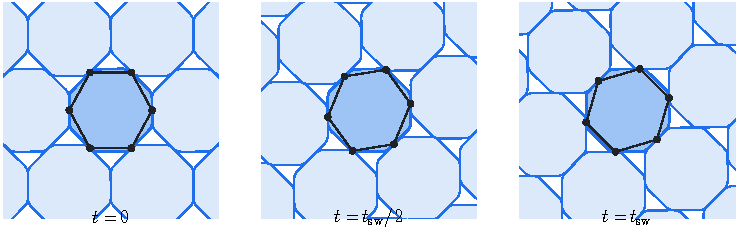
\includegraphics[width=\textwidth]{figures/fig-packing.pdf}
  \caption{Three densest lattice packings of the smoothed octagon. The dark copy touches six
  neighbours in each packing. The contact points move along its boundary as the packing lattice
  varies, while the density remains $\doct$.}
  \label{fig:packing}
\end{figure}

\begin{figure}[htbp]
  \centering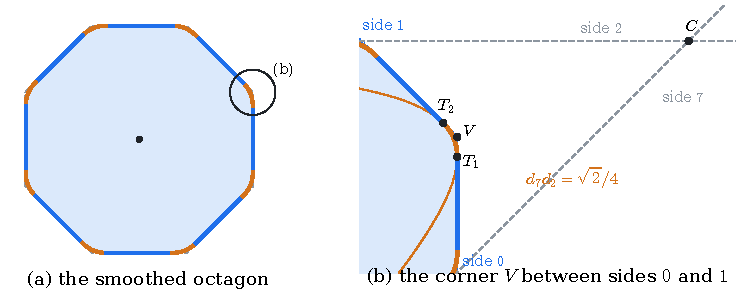
\includegraphics[width=\textwidth]{figures/fig-octagon.pdf}
  \caption{(a) The smoothed octagon: straight boundary segments (blue) and hyperbolic arcs
  (orange) inside the regular octagon (dashed). (b) One corner is replaced by the arc from $T_1$
  to $T_2$. The hyperbola is tangent to the two sides at these points and asymptotic to the
  neighbouring side lines, which meet at $C$. The coordinates are given in \cref{sec:set-octagon}.}
  \label{fig:octagon}
\end{figure}

\subsection{Why the geometric and control minima agree}\label{sec:setting-equivalence}

A \emph{global minimizer} is an admissible trajectory whose cost is no greater than that of any
other admissible trajectory, including trajectories with a different terminal time
(\cref{def:global-minimizer}). To use a cost bound for the packing problem, we must know that a
worst disk gives such a minimizer. Two geometric comparisons establish this.

First, a worst disk can be normalized and parametrized by an admissible trajectory whose cost is
$\sqrt{12}$ times its density (\cref{prop:realization}). Second, every admissible trajectory of
cost below $\pi$ traces a balanced disk with the same area (\cref{prop:reverse-comparison}). In
this second comparison the cost bound ensures that the contact curves go around the boundary
once, so that they describe a convex disk.

The octagon costs less than $\pi$. Any trajectory that could improve on the realization of a
worst disk would therefore also have cost below $\pi$, and would produce a disk with a smaller
packing density. This contradicts the choice of a worst disk. Its realization is consequently a
global minimizer. The same comparisons prove the equivalence between the lower bound for all
packing densities and the lower bound for all admissible costs (\cref{thm:equivalence}).

There is also a geometric restriction on the states that need to be considered. Hales and Vajjha
show that the state of every global minimizer lies in a fixed compact set, denoted $\hstarstar$
(\cref{thm:compact-domain}). In particular it stays away from the boundary of the allowed state
domain. This restriction will enter the last mixed case. The next section reduces the control
of a minimizer to a finite sequence of vertex choices.

\section{From minimizers to finite switching patterns}\label{sec:outline-periods}

An admissible control may take any value in the control triangle. A global minimizer, however, can
be represented by finitely many pieces of constant vertex control. We establish this
representation and classify its switching patterns. Excluding the longer patterns will leave at
most five pieces.

\subsection{Finiteness and normality}\label{sec:outline-reduction}

The \emph{Pontryagin maximum principle} gives necessary conditions for an optimal control. It
introduces auxiliary matrix-valued functions, called \emph{costates}, that measure the response of
the cost to variations of the trajectory. Together with the state and control, they form a
\emph{Pontryagin extremal} (\cref{def:pmp-extremal}). A scalar multiplier records the contribution
of the cost. The extremal is \emph{normal} when this multiplier is nonzero; it can then be
normalized to $-1$.

These necessary conditions do not by themselves give a finite switching description. At certain
states and costates, called the \emph{singular locus}, they fail to distinguish the available
controls. Such behaviour can lead to infinitely many switches in finite time. Our first estimate
uses the bound $\cost\le\Aoct<\pi$ to keep a minimizing extremal away from this locus
(\cref{prop:clearance}).

Away from the singular locus, one of the three vertex controls is locally excluded. The problem
then reduces locally to an edge of the control triangle. An edge minimizer has at most four
pieces (\cref{prop:edge-bound}). Covering the time interval by finitely many such neighbourhoods
gives a finite number of switches. After joining equal neighbouring pieces and choosing a switch
as the starting time, the minimizer has a \emph{vertex representation}: a finite sequence of
constant vertex controls with unequal neighbouring labels, including across the closing seam.
Finally, the closing conditions rule out a zero cost multiplier.

The resulting object is a \emph{normal vertex period}: an admissible trajectory with a vertex
representation and a normal Pontryagin extremal. It is \emph{competitive} when its cost is at
most $\Aoct$. The finite normal representation theorem (\cref{thm:finite-normal}) gives such a
period for every global minimizer. It has the same cost as the original trajectory and stays in
$\hstarstar$; only its starting time has changed.

The equality case requires this representation of the original disk's motion, including its change
of starting time. The precise reduction is proved in \cref{sec:reduction}.

\subsection{Data of a single piece}\label{sec:outline-pieces}

Let $N$ be the number of pieces. We write $\tau_k$ for their switching times and
$i_k\in\mathbb Z/3\mathbb Z$ for their labels, where labels are read cyclically as $0,1,2$.
The closing condition shifts every label by one after a period, so $i_{k+N}=i_k+1$.
For the octagon, the four labels are $2,0,1,2$; the next label is $0$, obtained by adding one to
the first label.

The state has three positive coordinates $p_0(X),p_1(X),p_2(X)$, called \emph{margins}, one for
each vertex control (\cref{lem:margins}). On a piece with label $i$, the coordinate $p_i(X)$ is
constant. It is the \emph{active margin} of that piece. Write $a_k$ for this constant on piece
$k$. It measures the scale of the state's motion during that piece. The other two margins, the
frame and the costate all have explicit evolution formulas.

A piece can therefore be specified by its starting data and one positive duration. The state and
frame must close after all the pieces have been composed. In these variables, closure is a finite
system of equations, and the maximum principle becomes a finite system of inequalities.
\Cref{sec:periods} derives the formulas and their consequences for the case arguments.

\subsection{The five switching patterns}\label{sec:outline-signs}

A switch is \emph{forward} if $i_{k+1}=i_k+1$ and \emph{reverse} if
$i_{k+1}=i_k-1$. Denote its sign by $+$ or $-$, respectively. These are the only possibilities
because consecutive labels are unequal. A \emph{run} is a maximal consecutive block of switches
with the same sign. The signs repeat after a period, so runs are understood cyclically. A period
is \emph{mixed} if it has both signs.

\begin{definition}[The five classes]\label{def:classes}
A vertex period is in class
\begin{itemize}
\item $\cls{R}$ if every switch is reverse;
\item $\cls{F}$ if every switch is forward;
\item $\cls{M3}$ if it is mixed and some reverse run has length other than two;
\item $\cls{M1}$ if it is mixed, every reverse run has length two and every forward run has
  length one, so its cyclic sign sequence is $(--+)^m$ for some positive integer $m$;
\item $\cls{M2}$ if it is mixed, every reverse run has length two and some forward run has
  length at least two.
\end{itemize}
\end{definition}

\begin{proposition}[Partition]\label{prop:partition}
Every vertex representation is in one of the classes $\cls{R}$, $\cls{F}$, $\cls{M3}$,
$\cls{M1}$, $\cls{M2}$.
\end{proposition}

In a mixed period, the maximum principle excludes reverse runs whose length differs from two. The
remaining patterns require comparisons with the cost of a complete period.

\subsection{A conserved quantity and the cost budget}\label{sec:outline-casimir}

The costates supply a quantity that links these local and global conditions. For the first
costate matrix $\Lambda_1(t)$, conjugation along the trajectory preserves its determinant. We
use the scaled invariant
\[
  \gamma^2=\frac{\det\Lambda_1(0)}{12},
\]
called the \emph{Casimir}. This notation does not assume positivity. Every mixed normal period has $\gamma^2>0$ (\cref{prop:ellipticity}).

The frame must turn through $\pi/3$ in a period. The cost of this turning gives an upper bound
for the Casimir: every competitive mixed period satisfies
\[
  \gamma^2<\frac5{27}.
\]
The cost--Casimir inequality and this consequence are proved in
\cref{prop:cost-casimir,cor:casimir-cap}. The entirely forward case uses a sharper bound of the
same kind.

The invariant can also be computed from the data adjacent to a single piece. In two of the case
arguments, these local data force a value of $\gamma^2$ exceeding the bound imposed by the cost. A
third case compares the turning accumulated at successive pieces with that required by closure.

\subsection{The bound on the number of pieces}\label{sec:outline-five}

\begin{theorem}[At most five pieces]\label{thm:at-most-five}
A competitive normal vertex period whose state stays in the compact domain $\hstarstar$ has at
most five pieces.
\end{theorem}

\Cref{sec:outline-classes} proves this theorem by excluding the five possible classes of longer
periods. The remaining periods admit a direct comparison with the octagon.
\section{Excluding six or more pieces}\label{sec:outline-classes}

By \cref{prop:partition}, \cref{thm:at-most-five} follows from one theorem for each of the five
classes. The five exclusions use different mechanisms. The classes $\cls{R}$ and $\cls{M3}$ are
excluded for every normal vertex period, with no reference to the cost: their obstructions are
local and come from the maximum principle alone. The classes $\cls{M1}$, $\cls{F}$ and $\cls{M2}$
are excluded only for competitive periods, through the Casimir cap and estimates over the whole
period. This section states the five theorems and explains their proofs, which are in
\cref{sec:reverse,sec:short-runs,sec:forward,sec:mixed,sec:smaller-short}.

\subsection{Classes R and M3}\label{sec:outline-reverse}

The two classes whose obstruction is local are an entirely reverse period and a mixed period with
a maximal reverse run of length other than two. Both exclusions rest on two facts about a few
consecutive pieces, which hold for every normal vertex period, whatever its cost and its number of
pieces. The first says that across three reverse switches the active margin of an interior piece
cannot be a minimum of the four.

\begin{lemma}[Reverse-four principle]\label{lem:reverse-four}
Let four consecutive pieces $k,\dots,k+3$ of a normal vertex period have three reverse switches
between them. Then
\begin{enumerate}[label=\textup{(\alph*)}]
\item it is not the case that $a_{k+2}\le a_k$, $a_{k+2}\le a_{k+1}$ and $a_{k+2}\le a_{k+3}$;
\item it is not the case that $a_{k+1}\le a_k$, $a_{k+1}\le a_{k+2}$ and $a_{k+1}\le a_{k+3}$.
\end{enumerate}
\end{lemma}

It is proved from two exact linear identities between the switching functions at the three
switches (\cref{lem:rev-identities}) and the sign of an explicit cost derivative
(\cref{lem:rev-N}). The second fact says that across two switches that return to the same label,
the active margins are strictly log-concave; it is read off the explicit switching function on the
middle piece.

\begin{lemma}[Three-arc log-concavity and turn ordering]\label{lem:three-arc}
Let $k,k+1,k+2$ be consecutive pieces of a normal vertex period.
\begin{enumerate}[label=\textup{(\alph*)}]
\item If $i_{k+2}=i_k$, then $a_ka_{k+2}<a_{k+1}^2$; in particular $a_{k+1}$ is not at most both
  $a_k$ and $a_{k+2}$.
\item If the switch $k$ is reverse and the switch $k+1$ forward, then $a_k<a_{k+2}$; if the switch
  $k$ is forward and the switch $k+1$ reverse, then $a_{k+2}<a_k$.
\end{enumerate}
\end{lemma}

An entirely reverse period has a global minimum of its active margins, and the four pieces around
it have three reverse switches between them; this contradicts \cref{lem:reverse-four}.

\begin{theorem}[Class $\cls{R}$]\label{thm:class-R}
No normal vertex period has every switch reverse.
\end{theorem}

In a reverse run of a mixed period, the two lemmas leave room for exactly one configuration: a run
of two switches around a strict minimum.

\begin{proposition}[Run structure]\label{prop:run-structure}
Let $P$ be a mixed normal vertex period, and let the switches $k,\dots,k+L-1$ form a maximal
reverse run. Then $L=2$, and the active margin of the centre piece $k+1$ is strictly smaller
than those of the four pieces around it:
\[
  a_{k+1}<a_{k-1},\qquad a_{k+1}<a_k,\qquad a_{k+1}<a_{k+2},\qquad a_{k+1}<a_{k+3}.
\]
\end{proposition}

\begin{theorem}[Class $\cls{M3}$]\label{thm:class-M3}
No normal vertex period is mixed with a maximal reverse run of length other than two.
\end{theorem}

\Cref{thm:class-M3} is the first conclusion of \cref{prop:run-structure}. The second conclusion,
the strict minimum at every centre, is the input of the remaining mixed classes, and of the proof
of ellipticity (\cref{prop:ellipticity}). The proofs are in \cref{sec:reverse}, and the identities
behind them in \cref{app:reverse-estimates}.

\subsection{Class M1}\label{sec:outline-short-runs}

A period of class $\cls{M1}$ is mixed, every maximal run of reverse switches has length two and
every maximal run of forward switches has length one. Its cyclic sign word is therefore
$(--+)^m$: every reverse run is a pair of reverse switches around a centre piece, and consecutive
pairs are separated by single forward switches.

\begin{theorem}\label{thm:class-M1}
  No competitive normal vertex period belongs to class \cls{M1}.
\end{theorem}

The theorem uses neither the compact domain nor a lower bound on the number of pieces. Its proof
compares two ways of counting how far the switch vectors $y_k$ turn in one period, measured in a
positive definite form $S$ built from the normal multiplier. At a turn the switch vector only
changes sign, so all the turning happens at the $m$ centres. A whole-period winding identity fixes
the total turning at exactly $(m+1)\pi/3$, because the frame of a competitive period turns by
exactly $\pi/3$ (\cref{prop:m1-winding}). A local estimate at each centre, which combines the
stationarity identity, the Gram identity and the Casimir cap, shows that each centre turns the
switch vectors by more than $2\pi/5$ (\cref{prop:m1-angle-gap}). The average $(m+1)\pi/(3m)$ is at
most $2\pi/5$ as soon as $m\ge5$, and the sign sum (\cref{lem:sign-sum}) leaves $m=2$ as the only
other case. With two centres the recurrence of the switch vectors closes up only in a rigid
configuration whose cost can be computed exactly, and it exceeds $\Aoct$
(\cref{prop:m1-two-centre}). The proof is in \cref{sec:short-runs}.

\subsection{Class F}\label{sec:outline-forward}

The smoothed octagon's period is entirely forward. No other entirely forward period with six or
more pieces is competitive.

\begin{theorem}[Class F]\label{thm:class-F}
No competitive normal vertex period with at least six pieces has every switch forward.
\end{theorem}

The proof plays two consequences of competitiveness against each other. On one side, the spectral
cost--Casimir inequality gives the sharper cap
$\gamma^2\le(3\Aoct/\pi-\frac32)^2/12$
(\cref{prop:fwd-spectral,cor:fwd-cap}). On the other side, $\gamma^2$ can be
read off at any piece from the two switch norms on either side of it and their cross pairing
(\cref{lem:gram}), and we read it at a piece of smallest active margin. In an entirely forward
period $N\equiv1\pmod3$, so a period with $N\ge6$ has at least seven pieces, and its cost is a sum
of seven or more edge terms that depend only on consecutive active margins. At the octagon's
margins each edge costs exactly a quarter of $\Aoct$, so seven edges fit into the budget only if
the smallest margin is markedly smaller than the octagon's. The switching conditions at the five
pieces around that small margin then hold the two switch norms close to their least possible value
$3/32$, and with such norms the Gram identity makes $\gamma^2$ slightly larger than
competitiveness allows. The central pairing retains a positive logarithmic correction; the resulting
vertex bounds for the Casimir exceed the spectral cap (\cref{fig:forward}). The proof is in \cref{sec:forward}, and its scalar estimates in
\cref{app:forward-estimates}.

\subsection{Class M2}\label{sec:outline-mixed}

A period of class $\cls{M2}$ has switches of both signs, every maximal reverse run has exactly two
switches, and some maximal forward run has at least two. Unlike the other classes, such a period
has no rigid sign word: the forward runs may have any lengths, the number of reverse runs is
arbitrary, and the factors are unrelated.

\begin{theorem}[Class $\cls{M2}$]\label{thm:class-M2}
Let $P$ be a competitive normal vertex period whose state stays in $\hstarstar$ and which has at
least six pieces. Then the sign sequence of $P$ is not of class $\cls{M2}$.
\end{theorem}

The exclusion is therefore local. We look at a window of at most seven consecutive pieces around
the smallest active margin of the period, read the normal multiplier of the whole period in that
window, and derive a finite list of scalar necessary conditions, which are then shown to be
inconsistent. The whole period enters only through three inputs: the compact domain, the Casimir
cap, and a lower bound on the Casimir obtained from the winding of the switch vectors over the
period. The first step locates the window.

\begin{proposition}[The minimum is a reverse centre]\label{prop:m2-centre}
Let $P$ be a competitive normal vertex period of class $\cls{M2}$ with at least six pieces. There is
an index $m$ with $a_m\le a_k$ for every $k$ such that the switches $m-1$ and $m$ are reverse and the
switches $m-2$ and $m+1$ are forward.
\end{proposition}

Of the two turns beside that centre we choose the one with the smaller active margin; after
reflecting the period and reversing time if necessary, it follows the centre
(\cref{lem:m2-reflection}). The forward run that starts at this turn has one switch or more.

If it has at least two, the run is \emph{nonshort}, and the switch after the next piece is forward
or reverse (\cref{prop:m2-window,prop:m2-continuation}). A comparison that moves one margin to a
boundary value turns the window into one scalar residual $N$ that must be negative
(\cref{lem:m2-comparison}), together with a short list of necessary bounds
(\cref{lem:m2-necessary}). A reverse successor contradicts $N<0$ directly (\cref{thm:m2-reverse}).
A forward successor leaves a small region of parameters on which the Casimir exceeds the cap
(\cref{thm:m2-forward}). \Cref{sec:mixed} gives this part of the proof, and
\cref{app:nonshort-estimates} its polynomial inequalities.

If the forward run has a single switch, it is a short bridge between two reverse runs. Its data
are fixed by six real numbers, and no free continuation of the period is left to compare with. The
proof works with a fixed list of necessary conditions on those numbers, the \emph{smaller-short
window} (\cref{def:ss-window}), and shows that the list is inconsistent
(\cref{thm:m2-smaller-short}). It proceeds through seven steps, which we call gates. Gates S0 to
S3 confine the shape of the bridge to a small box, gate S4 gives a lower bound for the Casimir,
gate S5 shows that the bridge is sheared in a definite direction, and gate S6 shows that a bridge
sheared in that direction costs more, together with the rest of the period, than the octagon.
\Cref{sec:smaller-short} gives this part of the proof, and \cref{app:short-estimates} its scalar
estimates.

\subsection{Proof of \texorpdfstring{\cref{thm:at-most-five}}{the bound on the number of pieces}}\label{sec:outline-five-proof}

\begin{proof}[Proof of \cref{thm:at-most-five}]
Suppose $N\ge6$. By \cref{prop:partition} the period is in one of the five classes, and each
class is excluded by a theorem proved in the following sections:
\begin{center}
\begin{tabular}{@{}lll@{}}
\toprule
Class & Excluded by & Hypotheses used\\
\midrule
$\cls{R}$ & \cref{thm:class-R} & none\\
$\cls{M3}$ & \cref{thm:class-M3} & none\\
$\cls{M1}$ & \cref{thm:class-M1} & competitive\\
$\cls{F}$ & \cref{thm:class-F} & competitive, $N\ge6$\\
$\cls{M2}$ & \cref{thm:class-M2} & competitive, state in $\hstarstar$, $N\ge6$\\
\bottomrule
\end{tabular}
\end{center}
Only the classes $\cls{F}$ and $\cls{M2}$ use the bound on the number of pieces.
\end{proof}

The classes $\cls{R}$ and $\cls{M3}$ are excluded for every normal vertex period, with no
reference to the cost: their obstructions are local in the period and come from the maximum
principle alone. The classes $\cls{M1}$, $\cls{F}$ and $\cls{M2}$ are excluded only for
competitive periods, through the Casimir cap and estimates over the whole period.
\Cref{sec:outline-terminal} treats the periods with at most five pieces.

\section{Five or fewer pieces, and the proofs of the main theorems}\label{sec:outline-terminal}

This section compares the periods with at most five pieces with the octagon, completes the proofs
of \cref{thm:control} and \cref{thm:main}(b), and then proves the equality case. The proofs of the
results stated here are in \cref{sec:terminal,sec:equality}.

\subsection{Periods with at most five pieces}\label{sec:outline-short}

For so few pieces nothing has to be estimated abstractly. The tangent closure
(\cref{lem:tangent-closure}) is a system of four scalar equations in the factors; with at most
five factors it either has no solution or determines the factors up to one or two parameters. It
leaves four pieces with every switch forward, and five pieces with the word $0\,1\,0\,2\,0$ or with
every switch reverse (\cref{prop:terminal-words}); the last are excluded by \cref{thm:class-R}. The
twist $X(T)=R^{-1}X(0)R$ then determines the initial state, and the cost becomes an explicit
function of the parameters.

The difficulty is that the comparison is sharp. The four-piece family is a curve $a^2+b^2=1$ that
contains the octagon at $a=b=1/\sqrt2$, so its minimum must be located exactly
(\cref{thm:four-density}); the sign of the derivative comes from a monotone weight and a lower
bound for the logarithm. The five-piece family approaches the octagon at the edge of its domain,
where one of its factors tends to~$1$ and the period degenerates into the octagon's four pieces.
Its strict inequality (\cref{thm:five-density}) therefore has no margin near that edge, and is
proved through a concave envelope in one variable.

\begin{theorem}[Terminal comparison]\label{thm:terminal}
Every normal vertex period with at most five pieces costs at least $\Aoct$.
\end{theorem}

\begin{proposition}[Terminal equality]\label{prop:terminal-equality}
Let $P$ be a normal vertex period with at most five pieces and cost $\Aoct$. Then $T=\tf$, and
there is $r\in\N$ such that, for $t\in[0,T]$,
\[
 R^{-r}g(t)R^{r}=g_{\mathrm{oct}}(t),\qquad R^{-r}X(t)R^{r}=X_{\mathrm{oct}}(t),
\]
where $(g_{\mathrm{oct}},X_{\mathrm{oct}})$ is the trajectory of the smoothed octagon
(\cref{prop:octagon-trajectory}).
\end{proposition}

\subsection{Proofs of the lower bounds}\label{sec:terminal-proofs}

The chain of reductions now closes. Recall that a global minimizer is an admissible trajectory
whose cost is at most that of every admissible trajectory (\cref{def:global-minimizer}).

\begin{theorem}[Cost of a minimizer]\label{thm:minimizer-cost}
Every global minimizer of the control problem costs at least $\Aoct$.
\end{theorem}

\begin{proof}
Let $(T,u,g,X)$ be a global minimizer. The octagon's trajectory is admissible and costs $\Aoct$
(\cref{prop:octagon-trajectory}), so $\cost(T,X)\le\Aoct$: the minimizer is competitive. By
\cref{thm:finite-normal}, rebased at a
switch it is a normal vertex period $P$ with the same terminal time and cost, whose state stays
in $\hstarstar$. By \cref{thm:at-most-five}, $P$ has at most five pieces, and by
\cref{thm:terminal}, $\cost(P)\ge\Aoct$.
\end{proof}

\begin{proof}[Proof of \cref{thm:control}]
Let $(T,u,g,X)$ be admissible, with any terminal time and any measurable control. By
\cref{thm:equivalence} a global minimizer $(T',u',g',X')$ exists: the realization of a worst disk.
By \cref{thm:minimizer-cost} and minimality, $\Aoct\le\cost(T',X')\le\cost(T,X)$, and
$\Aoct=\sqrt{12}\,\doct$.
\end{proof}

\begin{proof}[Proof of \cref{thm:main}\textup{(b)}]
By \cref{thm:equivalence} there is a worst disk $K_0$, a convex disk symmetric about the origin
whose greatest packing density is the least among all such disks, and its realization is a global
minimizer of cost $\sqrt{12}\,\delta(K_0)$. By \cref{thm:minimizer-cost},
$\sqrt{12}\,\delta(K_0)\ge\Aoct$, that is, $\delta(K_0)\ge\doct$. Now let $K$ be a convex disk with
a centre $c$, so that $2c-x\in K$ for $x\in K$. Its translate $K-c$ is a convex disk symmetric
about the origin, and translation does not change the greatest packing density, since a translate
is a congruent copy (\cref{prop:converse}). Hence $\delta(K)=\delta(K-c)\ge\delta(K_0)\ge\doct$.
\end{proof}


\subsection{The equality case}\label{sec:outline-equality}

\Cref{prop:terminal-equality} identifies a period of cost $\Aoct$ with the octagon's trajectory,
but only after three choices that the proof of the lower bound made along the way: the
normalization of the disk to Reinhardt's normal position, the rebasing of its trajectory at a
switch, and a relabeling of the vertices of the control simplex by a power of $R$. To classify the
disks of density $\doct$ these choices must be undone, and the trajectory to which the terminal
equality is applied must be the realization of the given disk; another minimizer of the same cost
would say nothing about it. Undoing the three choices and transporting the six arcs of the
octagon's trajectory back to the disk gives the following.

\begin{theorem}[Rigidity]\label{thm:rigidity}
Every worst disk is the image of the octagon $\KH$ under an invertible linear map of the plane.
Explicitly, with the notation of the proof, $K=e^{-1}g(s)R^{r}(\KH)$.
\end{theorem}

The converse is the affine invariance of the greatest packing density.

\begin{proposition}[Affine invariance]\label{prop:converse}
Let $K$ be a convex disk symmetric about the origin, $A$ an invertible linear map of the plane and
$b$ a vector. Then $\delta(AK)=\delta(K)$ and $\delta(K+b)=\delta(K)$. In particular
$\delta(A\KH)=\doct$ for every invertible linear map $A$.
\end{proposition}

Finally, the octagon $\KH$ of Hales's trajectory and Reinhardt's smoothed octagon $\Koct$ differ by
a linear map (\cref{fig:octagon}).

\begin{proposition}[Reinhardt's octagon is Hales's octagon]\label{prop:reinhardt-construction}
Let $A=\operatorname{diag}\bigl(1,(2\sqrt2-1)/\sqrt3\bigr)$. Then $A(\KH)=\Koct$.
\end{proposition}

\subsection{Proofs of parts (a) and (c) of \texorpdfstring{\cref{thm:main}}{the main theorem}}\label{sec:equality-proofs}

\begin{proof}[Proof of \cref{thm:main}\textup{(a)}]
By \cref{prop:reinhardt-construction}, $\Koct=A\KH$. The octagon $\KH$ is a compact convex set
with nonempty interior, symmetric about the origin, and $\delta(\KH)=\doct$
(\cref{prop:octagon-trajectory}); these properties pass to its linear image, the density by
\cref{prop:converse}.
\end{proof}

\begin{proof}[Proof of \cref{thm:main}\textup{(c)}]
Let $K$ be a convex disk with centre $c$. Suppose first that $\delta(K)=\doct$. The translate
$K-c$ is symmetric about the origin with $\delta(K-c)=\doct$, which by part~(b) is the least
value; so $K-c$ is a worst disk. By
\cref{thm:rigidity}, $K-c=L\KH$ for an invertible linear map $L$, and $K$ is the image of $\KH$
under the affine map $x\mapsto Lx+c$. Conversely, an affine image $A'\KH$, with linear part $L$,
is the translate $L\KH+A'(0)$, which has density $\doct$ by \cref{prop:converse}. This proves the
equivalence with $\KH$ in place of $\Koct$, and the affine images of $\KH$ are those of $\Koct$
by \cref{prop:reinhardt-construction}.
\end{proof}

In Hales's form, the equality disks are the affine images of the convex hull of the six arcs
$g(t)s_j$, $t\in[0,\tf]$, of the trajectory $(g,X)$ of the octagon's control from $g(0)=I$ and
$X(0)=\Phi(0,y_0)$ (\cref{prop:octagon-trajectory}); this hull is a centrally symmetric convex
disk of area $\Aoct=\sqrt{12}\,\doct$ and greatest packing density $\doct$. The equality data are
explicit: four
forward pieces with the word $\ee_2\ee_0\ee_1\ee_2$, every factor equal to $\sqrt2$, every
duration equal to $\log2/(2\sqrt{2\sqrt2-1})$, and initial state $\Phi(0,y_0)$.


\appendix
\crefalias{section}{appendix}
\crefalias{subsection}{appendix}
\crefalias{subsubsection}{appendix}
\crefname{appendix}{Appendix}{Appendices}
\Crefname{appendix}{Appendix}{Appendices}
\subsection{Outline of the finite reduction}\label{app:reduction-outline}

\Cref{sec:setting} produced a global minimizer of the control problem whose state stays in the
compact domain $\hstarstar$. This section shows that, after a change of origin in time, such a
minimizer has a control that takes only the three vertex values $\ee_0,\ee_1,\ee_2$, switching
finitely often in a period, and that it carries a Pontryagin lift with cost multiplier
$\lambda=-1$. The conclusion is \cref{thm:finite-normal}. Every later section starts from it.

The steps are the following. The maximum principle gives a lift $(\Lambda_1,\Lambda_R,\lambda)$ of
the minimizer, possibly abnormal ($\lambda=0$). The danger is the singular locus, where the
Hamiltonian does not depend on the control and the maximum condition gives no information. Near it
Hales and Vajjha find Fuller's system~\cite{HalesVajjha2024,Fuller1963}, whose optimal controls
switch infinitely often in finite time. A budget inequality, which uses only that the cost is at
most $\Aoct<\pi$, keeps every lift away from the singular locus in proportion to its size
(\cref{prop:clearance}). Away from the singular locus one vertex is excluded on each side of every
time (\cref{red:local-exclusion}). On an interval where one vertex is excluded the control runs
along an edge of the simplex, and an edge minimizer has at most four pieces
(\cref{prop:edge-bound}). Compactness of $[0,T]$ then gives finitely many pieces
(\cref{prop:finite-switches}). Merging equal neighbours and restarting the period at a genuine
switch gives a vertex representation (\cref{lem:word-reduction}), and for a lift of a trajectory
with a vertex representation the multiplier is nonzero (\cref{thm:normality}).

The order matters. The clearance and the switch count are homogeneous in
$(\lambda,\Lambda_1,\Lambda_R)$, so they hold for abnormal lifts as well as normal ones. The
normality argument, on the other hand, reads the costate at the finitely many switching times
and uses the twisted closing condition of the period. Finiteness is therefore proved first, for an
arbitrary lift, and normality afterwards.

\subsection{Pontryagin extremals}\label{red:extremals}

The maximum principle is applied to the problem of \cref{def:control-problem} with free terminal
time and with the closing conditions $g(0)=I$, $g(T)=R$, $X(T)=R^{-1}X(0)R$. Its conclusions, in
the form of Hales and Vajjha's Problem~6.7.1~\cite{HalesVajjha2024}, define the following object.

\begin{definition}[Pontryagin extremal]\label{def:pmp-extremal}
Let $(T,u,g,X)$ be a state trajectory (\cref{def:control-problem}) with $g(0)=I$, $g(T)=R$ and
$X(T)=R^{-1}X(0)R$. A \emph{Pontryagin lift} of it consists of two curves
$\Lambda_1,\Lambda_R\colon[0,T]\to\sltwo$ and a constant $\lambda\le0$, the \emph{cost
multiplier}, such that
\begin{enumerate}
\item $\ip{\Lambda_R(t)}{X(t)}=0$ and $(\lambda,\Lambda_1(t),\Lambda_R(t))\ne0$ for every
  $t\in[0,T]$;
\item $\Lambda_1$ and $\Lambda_R$ are absolutely continuous and satisfy, for almost every $t$,
  \begin{equation}\label{red:costate}
  \Lambda_1'=[\Lambda_1,X],\qquad
  \Lambda_R'=[P_u,\Lambda_R]-\ip{\Lambda_R}{P_u}[P_u,X]+[-\Lambda_1+\tfrac32\lambda J,X],
  \end{equation}
  with $P_u=Z_u/\ip{Z_u}{X}$ as in \cref{eq:state};
\item for almost every $t\in(0,T)$ the control $u(t)$ maximizes over $\UT$ the Hamiltonian
  \begin{equation}\label{red:hamiltonian}
  H(\Lambda_1,\Lambda_R,X;v)=\ip{\Lambda_1-\tfrac32\lambda J}{X}
  -\frac{\ip{\Lambda_R}{Z_v}}{\ip{X}{Z_v}},
  \end{equation}
  evaluated at $(\Lambda_1(t),\Lambda_R(t),X(t))$, and the maximum is $0$;
\item $\Lambda_1(T)=R^{-1}\Lambda_1(0)R$ and $\Lambda_R(T)=R^{-1}\Lambda_R(0)R$.
\end{enumerate}
The tuple $(T,u,g,X,\Lambda_1,\Lambda_R,\lambda)$ is a \emph{Pontryagin extremal}. It is \emph{normal} if $\lambda\ne0$ and
\emph{abnormal} if $\lambda=0$.
\end{definition}

Here $\Lambda_1$ is the costate of the frame, read in the left trivialization of $\SLtwo$, and
$\Lambda_R=[\Lambda_2,X]$ is the part of the costate of the state that the dynamics see. The
conditions are positively homogeneous in $(\Lambda_1,\Lambda_R,\lambda)$, so a normal lift can be
rescaled to $\lambda=-1$.

\begin{theorem}[Pontryagin lift]\label{thm:pmp-lift}
Every global minimizer $(T,u,g,X)$ of the control problem (\cref{def:global-minimizer}) has a
Pontryagin lift $(\Lambda_1,\Lambda_R,\lambda)$.
\end{theorem}

Hales and Vajjha use this statement in the proof of their Proposition~8.1.3. It follows from the
maximum principle with free terminal time~\cite{Pontryagin1962,AgrachevSachkov2004}, applied on the
open subset of $\R^{2\times2}\times\sltwo$ cut out by $\det g>0$ and the star inequalities, with
the costates read through the left trivialization. The nontriviality of the reduced costate
$(\lambda,\Lambda_1,\Lambda_R)$ needs a separate argument: if $\lambda=0$ and $\Lambda_1$,
$\Lambda_R$ vanish at one time, then $\Lambda_1\equiv0$ by the conservation law below, and the
equation for $\Lambda_R$ becomes linear and homogeneous, so $\Lambda_R\equiv0$.

Two consequences of the costate equations are used throughout. The first is the conservation law
of Hales and Vajjha's Corollary~6.5.3,
\begin{equation}\label{red:conservation}
\Lambda_1(t)=g(t)^{-1}\Lambda_1(0)\,g(t)\qquad(0\le t\le T)
\end{equation}. In particular $\det\Lambda_1$ is constant. The second
concerns the three \emph{vertex Hamiltonians} $H_i(t)=H(\Lambda_1(t),\Lambda_R(t),X(t);\ee_i)$.
The denominator $-\ip{X}{Z_v}$ is positive and affine in $v$, and
$-\ip{X}{Z_v}\bigl(H(\cdot\,;v)-c\bigr)$ is affine in $v$ for every constant $c$. So the maximum of
$H$ over the simplex is attained at a vertex, and a vertex carrying positive weight in a maximizing
control is itself maximizing.

\begin{lemma}[Vertex Hamiltonians]\label{lem:vertex-hamiltonians}
For a Pontryagin extremal the vertex Hamiltonians $H_0,H_1,H_2$ are continuous on $[0,T]$, and at
every $t\in[0,T]$, not only almost every $t$, all three are $\le0$ and one of them is $0$.
\end{lemma}

\begin{proof}
Continuity holds because $X$, $\Lambda_1$, $\Lambda_R$ are continuous and $\ip{X}{Z_{\ee_i}}<0$ on
star states. By the maximum condition, $\max_iH_i(t)=0$ for almost every $t$, hence for every $t$
by continuity of $\max_iH_i$.
\end{proof}

\Cref{fig:red-hamiltonians} shows the three vertex Hamiltonians along the smoothed octagon's
period, for its normal lift.

\begin{figure}[htbp]
\centering
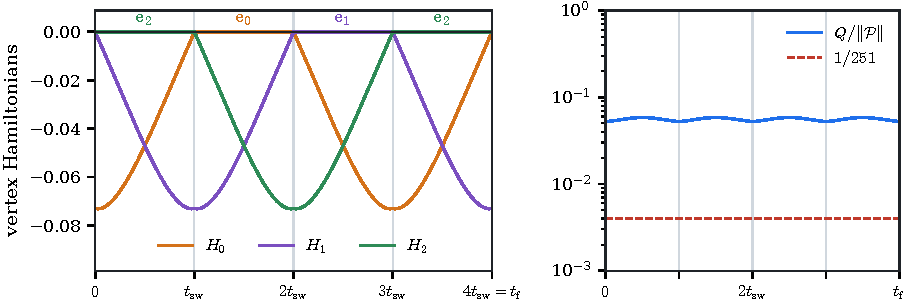
\includegraphics[width=\textwidth]{figures/fig-reduction-hamiltonians.pdf}
\caption{The normal Pontryagin lift ($\lambda=-1$) of the smoothed octagon's trajectory over one
period $[0,\tf]$, with control word $\ee_2\ee_0\ee_1\ee_2$ and switching time $\tsw=\tf/4$; the
lift is that of Hales and Vajjha's Theorem~7.5.1~\cite{HalesVajjha2024}, integrated numerically.
Left: the vertex Hamiltonians $H_0,H_1,H_2$. All three are $\le0$, the vertex of the current piece
has $H_i=0$, and at each switch the incoming vertex reaches $0$. Right: the ratio
$Q/\norm{\mathcal P}$ of \cref{prop:clearance}, on a logarithmic scale. It stays above the
uniform positive lower bound supplied by that proposition. The computation
confirms the closing conditions $\Lambda_1(\tf)=R^{-1}\Lambda_1(0)R$ and
$\Lambda_R(\tf)=R^{-1}\Lambda_R(0)R$ and every property stated here.}
\label{fig:red-hamiltonians}
\end{figure}

\runin{The singular locus.} If the three vertex Hamiltonians are equal at some time, then the maximum
condition at that time says nothing about the control. Hales and Vajjha's Lemma~8.2.1 identifies
when this happens.

\begin{lemma}[Singular locus]\label{red:singular-locus}
Let $X$ be a star state and $\Lambda_R$ traceless with $\ip{\Lambda_R}{X}=0$. Then
$H(\Lambda_1,\Lambda_R,X;\ee_0)=H(\Lambda_1,\Lambda_R,X;\ee_1)=H(\Lambda_1,\Lambda_R,X;\ee_2)$ if
and only if $\Lambda_R=0$. If
$\Lambda_R\ne0$, there is a coordinate $i$ such that $v_i=0$ for every control $v$ maximizing $H$
over $\UT$.
\end{lemma}

So all three vertices tie at a time where $\Lambda_R=0$; if the Hamiltonian also vanishes there,
then $\ip{\Lambda_1-\frac32\lambda J}{X}=0$. The \emph{singular locus} is the set of costates with
$\Lambda_1=\frac32\lambda J$ and $\Lambda_R=0$; there $H(\cdot\,;v)=0$ for every control $v$. Put
\[
A=\Lambda_1-\tfrac32\lambda J,\qquad
\norm{\mathcal P}^2=\lambda^2+\norm{\Lambda_1}^2+\norm{\Lambda_R}^2,\qquad
Q^2=\norm{A}^2+\norm{\Lambda_R}^2,
\]
with Frobenius norms. Here $\mathcal P=(\lambda,\Lambda_1,\Lambda_R)$ is the extended covector,
and $Q$ is its distance from the singular locus.

\subsection{Singular clearance}\label{red:clearance-sec}

The singular locus cannot be excluded by local considerations; the argument uses the whole
period and its cost. Write $\omega(Y)=-\frac12\ip{J}{Y}$. For a star state $\omega(Y)\ge1$, and
the cost density is $-\frac32\ip{J}{X}=3\omega(X)$, so $\cost(T,X)=3\int_0^T\omega(X)$. For a
frame $h$ with $\det h=1$ put $\omega_R(h,Y)=\omega(hYh^{-1})$, the same quantity for the state
seen in the fixed frame.

\begin{lemma}[Winding]\label{red:winding}
For every admissible trajectory $(T,u,h,Y)$, with $h(0)=I$ and $h(T)=R$,
\[
\int_0^T\bigl(\omega(Y)+\omega_R(h,Y)\bigr)\,\dd t\ \ge\ \frac{2\pi}3.
\]
\end{lemma}

\begin{proof}
Write $\zeta(h)=\frac12(h_{00}+h_{11})+\frac i2(h_{10}-h_{01})\in\mathbb C$, the coefficient of
$h$ on the rotations. Since $\det h=1$, $\abs{\zeta(h)}\ge1$, and a direct computation gives
$\omega(Y)+\omega_R(h,Y)=2\operatorname{Im}\bigl(\overline{\zeta}\,\zeta'\bigr)$ along $h'=hY$. Let $L(t)=\int_0^t\zeta'/\zeta$, so that $\zeta=e^{L}$. Then
$\operatorname{Im}(\zeta'/\zeta)=(\omega+\omega_R)/(2\abs\zeta^2)>0$, and
$\zeta(T)=\zeta(R)=e^{i\pi/3}$ forces $\operatorname{Im}L(T)\in\frac\pi3+2\pi\Z$; being positive,
it is at least $\pi/3$. Since $\abs\zeta\ge1$,
$\int_0^T(\omega+\omega_R)=2\int_0^T\abs\zeta^2\operatorname{Im}(\zeta'/\zeta)
\ge2\operatorname{Im}L(T)\ge2\pi/3$.
\end{proof}

The second ingredient is pointwise: at a star state the control $u^*$ with $P_{u^*}=-X/2$ lies
in the simplex and has $H(u^*)=\ip{A}{X}$, so the maximum condition gives $\ip{A}{X}\le0$. The
weights of $u^*$ also bound $\Lambda_R$.

\begin{lemma}[Equilibrium inequality]\label{red:equilibrium}
Let $X$ be a star state, $\Lambda_R$ traceless with $\ip{\Lambda_R}{X}=0$, and suppose that every
vertex Hamiltonian at $(\Lambda_1,\Lambda_R,X)$ is $\le0$. Then $\ip{A}{X}\le0$. On each compact
set of star states there is a constant $C$ such that
$\norm{\Lambda_R}\le C\bigl(-\ip{A}{X}\bigr)$.
\end{lemma}

\begin{proof}
With $\varsigma_i=\sqrt3\ip{\Lambda_R}{Z_{\ee_i}}$ and the margins $p_i$ of \cref{lem:margins}, the
vertex Hamiltonians are $H_i=\ip{A}{X}+\varsigma_i/p_i$. The weights $\vartheta_i=p_i(p_j+p_k)/8$,
$\{i,j,k\}=\{0,1,2\}$, sum to $1$ by $p_0p_1+p_1p_2+p_2p_0=4$, and
$\sum_i\vartheta_i\varsigma_i/p_i=\frac18\sum_i(p_j+p_k)\varsigma_i
=\frac12\ip{\Lambda_R}{X}=0$. Hence $\ip{A}{X}=\sum_i\vartheta_iH_i\le0$. Put $m=-\ip{A}{X}\ge0$. From
$H_i\le0$, $(p_j+p_k)\varsigma_i\le8m\vartheta_i$. Since the three products
$(p_j+p_k)\varsigma_i$ sum to zero, each is at least the negative of the upper bounds for the
other two, hence at least $-8m(1-\vartheta_i)\ge-8m$; its upper bound is also at most $8m$.
On a compact set of star states every $p_j+p_k$ has a positive lower bound. Thus every
$\abs{\varsigma_i}$ is bounded by a fixed multiple of $m$. The matrices $Z_{\ee_i}$ span
$\sltwo$, and the trace form on $\sltwo$ is nondegenerate, so the linear map
$\Lambda_R\mapsto(\varsigma_0,\varsigma_1,\varsigma_2)$ is invertible. Its inverse has bounded
norm, proving the assertion.
\end{proof}

Only the strict gap between the octagon's cost and the circular cost enters the next estimate.
For $0\le c<\pi$ write
\[
 b(c)=\frac{2\pi-c}{3(\pi-c)},\qquad b_{\mathrm{oct}}=b(\Aoct).
\]
The function $b$ is increasing, and it is finite precisely while the cost stays below $\pi$.

\begin{proposition}[Budget inequality]\label{red:budget}
Let $(T,u,h,Y)$ be admissible with $\cost(T,Y)\le\Aoct$, let $M\in\R^{2\times2}$ and $\mu\in\R$, and
suppose $\ip{h(t)^{-1}Mh(t)+\frac32\mu J}{Y(t)}\le0$ for $t\in[0,T]$. Then
$\mu\le b_{\mathrm{oct}}\,\norm{M+\frac32\mu J}$. Consequently every Pontryagin
extremal with cost at most $\Aoct$ satisfies
\[
\abs\lambda\le b_{\mathrm{oct}}\,\bigl\lVert\Lambda_1(t)-\tfrac32\lambda J\bigr\rVert
\qquad(0\le t\le T).
\]
\end{proposition}

\begin{proof}
Put $A_0=M+\frac32\mu J$, $a_0=\norm{A_0}$ and $V=hYh^{-1}$. The hypothesis reads
$\ip{A_0}{V}+3\mu\,\omega_R\le3\mu\,\omega$. By the Cauchy--Schwarz inequality and
$\norm{V}^2=4\omega_R^2-2$, $\ip{A_0}{V}\ge-2a_0\omega_R$, so
$(3\mu-2a_0)\omega_R\le3\mu\,\omega$ pointwise. Let $c=\cost(T,Y)$,
$I=\int\omega=c/3$ and $I_R=\int\omega_R$. If $3\mu\le2a_0$, then
$\mu\le2a_0/3\le b(c)a_0$. Otherwise $3\mu-2a_0>0$, so integrating and using
$I_R\ge2\pi/3-I$ from \cref{red:winding} gives
\[
 (3\mu-2a_0)(2\pi-c)\le3\mu c,
 \qquad\text{hence}\qquad
 3\mu(\pi-c)\le a_0(2\pi-c).
\]
Since $c\le\Aoct<\pi$, division gives $\mu\le b(c)a_0\le b_{\mathrm{oct}}a_0$.
For the consequence, rebase
the twisted extension of the extremal at $t$ (\cref{red:rebase}). The rebased trajectory is
admissible with the same cost, its costate at time $0$ is $\Lambda_1(t)$ by \cref{red:conservation},
and \cref{red:equilibrium} gives the hypothesis with $M=\Lambda_1(t)$ and $\mu=-\lambda$.
\end{proof}

The gap $\pi-\Aoct>0$ is what makes the budget effective. It bounds the
multiplier by the distance $\norm{A}$ from $\Lambda_1$ to $\frac32\lambda J$; adding
$\norm{\Lambda_R}$ gives the clearance.

Put
\[
 c_{\mathrm{oct}}=
 \sqrt{b_{\mathrm{oct}}^2+\bigl(1+3b_{\mathrm{oct}}/\sqrt2\bigr)^2}.
\]

\begin{proposition}[Singular clearance]\label{prop:clearance}
Let $(T,u,g,X,\Lambda_1,\Lambda_R,\lambda)$ be a Pontryagin extremal, normal or abnormal, with
$\cost(T,X)\le\Aoct$ and $X(t)\in\hstarstar$ for $t\in[0,T]$. Then
\[
\norm{\mathcal P(t)}\le c_{\mathrm{oct}}\,Q(t)\qquad(0\le t\le T).
\]
In particular $Q(t)>0$ for every $t$: the costate never meets the singular locus.
\end{proposition}

\begin{proof}
Write $\Lambda_1=A+\frac32\lambda J$. Since $\norm{J}=\sqrt2$, the triangle inequality and
\cref{red:budget} give
\[
 \norm{\Lambda_1}\le\norm{A}+\frac3{\sqrt2}\abs\lambda
 \le\bigl(1+3b_{\mathrm{oct}}/\sqrt2\bigr)\norm{A}.
\]
Consequently
$\norm{\mathcal P}^2\le c_{\mathrm{oct}}^2\norm{A}^2+\norm{\Lambda_R}^2
\le c_{\mathrm{oct}}^2Q^2$, since $c_{\mathrm{oct}}>1$.
The positivity of $Q$ follows from the nontriviality
$\norm{\mathcal P}>0$.
\end{proof}

\begin{remark}\label{red:clearance-remark}
These estimates are uniform on each compact set $K$ of star states. By
\cref{red:equilibrium} and the boundedness of $\norm X$ on $K$, there is $D_K\ge0$ such that
$\norm{\Lambda_R}^2\le D_K\norm A^2$. Put $F=2e^{2\Aoct/3}$. Along $g'=gX$,
\[
 \frac{\dd}{\dd t}\norm g^2=2\tr(Xg^{\mathsf T}g)
 \le2\omega(X)\norm g^2,
\]
so Gronwall's inequality gives $\norm{g(t)}^2\le F$. Since
$\norm{g^{-1}}=\norm g$ for $\det g=1$, spatial conservation
(\cref{red:conservation}) bounds $\norm{\Lambda_1(t)}^2$ by
$F^2\norm{\Lambda_1(0)}^2$ and conversely. Together with
$\norm A^2\le2\norm{\Lambda_1}^2+9\lambda^2$, this yields
\[
 G_K^{-1}\norm{\mathcal P(0)}^2\le\norm{\mathcal P(t)}^2
 \le G_K\norm{\mathcal P(0)}^2,
 \qquad G_K=(1+9D_K)+(1+2D_K)F^2.
\]
The constant depends only on $K$ and $\Aoct$.
\end{remark}

\subsection{The edge bound}\label{red:edge-sec}

Suppose that on a time interval one coordinate of the control vanishes almost everywhere, say
$u_0=0$. The trajectory then runs along the edge of the simplex opposite $\ee_0$, and the control is
determined by one number $v=u_1\in[0,1]$. A priori $v$ could still alternate between the two
remaining vertices infinitely often. The following bound excludes this for a global minimizer.

\begin{proposition}[Edge bound]\label{prop:edge-bound}
Let $(T,u,g,X)$ be a global minimizer, $0\le t_0<t_1\le T$, and $j\in\{0,1,2\}$ with $u_j=0$ almost
everywhere on $(t_0,t_1)$. Then on $[t_0,t_1]$ the control is almost everywhere a concatenation of
at most four constant vertex pieces of positive length.
\end{proposition}

\begin{proof}
Relabeling by a power of $R$ (\cref{red:rebase}) moves the missing vertex to $j=0$ and keeps
minimality. On the edge, a star state $X=\bigl(\begin{smallmatrix}a&b\\c&-a\end{smallmatrix}\bigr)$
has $b=-(1+a^2)/c$, and the star inequalities read $c>0$, $3a^2<c^2<3(1+a^2)$. With
$u=(0,v,1-v)$ and $\alpha=(2v-1)/\sqrt3$, the state equation becomes the control system
\[
a'=\frac{c}{c-3\alpha a},\qquad c'=\frac{3\alpha c}{c-3\alpha a},\qquad s'=c,
\]
in the state $(a,c,s)$, $s=\int c$, with cost density $\frac32\bigl(c+(1+a^2)/c\bigr)$. The frame is recovered from $x=a/c$ and $s$. Replacing the segment $[t_0,t_1]$ of the minimizer by any
edge trajectory with the same end states and end frames, and translating the rest of the
trajectory in time, gives an admissible trajectory whose cost changes by the difference of the
segment costs. Since competitors with any terminal time are
allowed, the segment minimizes the edge cost among edge trajectories with its end points and free
duration.

The maximum principle with free time applies to this system on the open set given by the star
inequalities. It gives a multiplier $\nu\le0$ and a covector $p=(p_a,p_c,p_s)$ with
$(\nu,p(t))\ne0$ and $H=0$, and $p_s$ is constant since the system does not depend on $s$. The
derivative of the Hamiltonian in $\alpha$ is $3c\,\varsigma/(c-3\alpha a)^2$ with the
\emph{switching function} $\varsigma=ap_a+cp_c$, so $v=1$ where $\varsigma>0$ and $v=0$ where
$\varsigma<0$. The adjoint equation, the homogeneity of the field in $(a,c)$ and $H=0$ give
\[
\varsigma'=-c\,\bigl(2p_s+3\nu(1+x^2)\bigr),\qquad x=a/c,\quad x'=1/c>0.
\]
Since $x$ is strictly increasing, the quadratic $2p_s+3\nu(1+x^2)$ vanishes at most twice in time
unless $\nu=p_s=0$; then $\varsigma$ has at most three zeros by Rolle's theorem, and the control
has at most four constant pieces. If $\nu=p_s=0$, then $\varsigma$ is constant, and it is nonzero,
because $\varsigma=0$ and $H=0$ would force $p=0$.
\end{proof}

\subsection{Finitely many switches}\label{red:switch-sec}

\begin{lemma}[Local exclusion of a vertex]\label{red:local-exclusion}
Let $(T,u,g,X,\Lambda_1,\Lambda_R,\lambda)$ be a Pontryagin extremal with $X(t)\in\hstarstar$ on
$[0,T]$, and let $t_0\in[0,T]$ with $Q(t_0)>0$. There are $\delta>0$ and vertices $j,k$ such that
$H_j<0$ on $(t_0,t_0+\delta)\cap[0,T]$ and $H_k<0$ on $(t_0-\delta,t_0)\cap[0,T]$.
\end{lemma}

\begin{proof}
If $H_i(t_0)<0$ for some $i$, continuity gives the claim with $j=k=i$. Otherwise all three vertex
Hamiltonians vanish at $t_0$ (\cref{lem:vertex-hamiltonians}), so $\Lambda_R(t_0)=0$ by
\cref{red:singular-locus} and $\ip{A}{X}=0$ there. Then $Q(t_0)>0$ gives $A(t_0)\ne0$, and
$b=[X(t_0),A(t_0)]\ne0$, since a traceless matrix commuting with $X$ is a multiple of $X$ and
$\ip{X}{X}=-2$. The control-dependent terms of \cref{red:costate} are $O(\norm{\Lambda_R})$, so
$\Lambda_R'(t_0)=b$, and $h_i=\ip{\Lambda_R}{Z_{\ee_i}}/\ip{X}{Z_{\ee_i}}$ has derivative
$c_i=\ip{b}{Z_{\ee_i}}/\ip{X}{Z_{\ee_i}}$ at $t_0$. As $b$ is traceless and orthogonal to $X$,
\cref{red:singular-locus} applied to $b$ shows that the $c_i$ are not all equal. If $c_k<c_j$, then
$H_j-H_k=h_k-h_j$ vanishes at $t_0$ with negative derivative, so $H_j<H_k\le0$ just after $t_0$ and
$H_k<H_j\le0$ just before.
\end{proof}

Where $H_j<0$ on an interval, the coordinate $u_j$ of the control vanishes almost everywhere there,
because a vertex with positive weight in a maximizing control is maximizing. So the edge bound applies on both sides of $t_0$.

\begin{proposition}[Finitely many switches]\label{prop:finite-switches}
Let $(T,u,g,X,\Lambda_1,\Lambda_R,\lambda)$ be a Pontryagin extremal with $\cost(T,X)\le\Aoct$ and
$X(t)\in\hstarstar$ on $[0,T]$, satisfying the clearance of \cref{prop:clearance}, and whose control
has the property of \cref{prop:edge-bound}. Then there is $n$ such that on $[0,T]$ the control is
almost everywhere a concatenation of $n$ constant vertex pieces of positive length.
\end{proposition}

\begin{proof}
By \cref{prop:clearance}, $Q(t_0)>0$ at every $t_0$. \Cref{red:local-exclusion} and the edge bound
give, around each $t_0$, a $\delta>0$ such that every subinterval of $[0,T]$ inside
$(t_0-\delta,t_0+\delta)$ has a finite vertex description: on the part after $t_0$ the vertex $j$
is missing and \cref{prop:edge-bound} gives at most four pieces, on the part before $t_0$ the vertex
$k$ is missing, and the two descriptions concatenate at $t_0$. A Lebesgue number of this cover of
the compact interval $[0,T]$ and induction along a uniform partition give a finite description of
$[0,T]$.
\end{proof}

\subsection{Vertex representations and rebasing}\label{red:rebase}

\begin{definition}[Vertex representation]\label{def:vertex-representation}
A \emph{vertex representation} of a control $u$ on $[0,T]$ consists of an integer $N\ge1$, a
strictly increasing sequence $(\tau_k)_{k\in\Z}$ of \emph{switching times} with $\tau_0=0$ and
$\tau_{k+N}=\tau_k+T$, and \emph{labels} $i_k\in\Z/3$ with $i_{k+N}=i_k+1$ and $i_{k+1}\ne i_k$ for
every $k\in\Z$, such that for $0\le k<N$ the control equals $\ee_{i_k}$ almost everywhere on
$(\tau_k,\tau_{k+1})$. The interval $(\tau_k,\tau_{k+1})$ is the
$k$-th \emph{piece}, and $N$ is the number of pieces of the period.
\end{definition}

\begin{definition}[Normal period]\label{def:normal-period}
A \emph{normal period} is a Pontryagin extremal $(T,u,g,X,\Lambda_1,\Lambda_R,\lambda)$ with
$\lambda=-1$, together with a vertex representation of its control $u$. It is
\emph{competitive} if $\cost(T,X)\le\Aoct$, and it lies in the
compact domain if $X(t)\in\hstarstar$ for $t\in[0,T]$. The
\emph{active margin} of the $k$-th piece is $a_k=p_{i_k}(X(\tau_k))$, with $k$ read modulo $N$.
\end{definition}

The pieces of \cref{prop:finite-switches} may have equal neighbouring labels, and the cut at $t=0$
need not be a switch. Both are repaired by extending the trajectory periodically. The \emph{twisted
extension} of an admissible trajectory $(T,u,g,X)$ is defined for $t\ge0$ by
\[
G(t)=g(t-nT)R^n,\qquad Y(t)=R^{-n}X(t-nT)R^n,\qquad n=\lfloor t/T\rfloor,
\]
and with the control $v(t)$ equal to $u(t-nT)$ with its coordinates shifted $n$ times, so that
the vertex $\ee_i$ becomes $\ee_{i+n}$ and $Z_{v(t+T)}=R^{-1}Z_{v(t)}R$. The extension satisfies the state equations
on every interval $[0,nT]$. The trajectory \emph{rebased} at $s\in[0,T)$ is, for $0\le t\le T$,
\[
\hat g(t)=G(s)^{-1}G(s+t),\qquad \hat X(t)=Y(s+t),\qquad \hat u(t)=v(s+t).
\]
It is again admissible, and it has the same cost because $J$ commutes with $R$; so a rebased global
minimizer is a global minimizer. Similarly the
\emph{relabeling} $(g,X)\mapsto(R^{-r}gR^r,R^{-r}XR^r)$, with the control coordinates shifted $r$
times, preserves admissibility and cost.



In a vertex representation (\cref{def:vertex-representation}), the condition $i_{k+1}\ne i_k$ for every $k$, including $k=N-1$, says that equal neighbours have
been merged also across the seam $t=T$, where the label after the last piece is $i_N=i_0+1$.

\begin{lemma}[Merging and rebasing]\label{lem:word-reduction}
If on $[0,T]$ the control $u$ is almost everywhere a concatenation of $n$ vertex pieces, there is
$s\in[0,T)$ such that the rebased control $\hat u$ has a vertex representation with $N\le n$ pieces.
\end{lemma}

\begin{proof}
Extend the pieces by the twist to a bi-infinite sequence with $\tau_{k+n}=\tau_k+T$ and labels
$l_{k+n}=l_k+1$. Call $\tau_k$ a genuine switch if $l_k\ne l_{k-1}$. The increments
$l_k-l_{k-1}$ over one period sum to $1\ne0$ in $\Z/3$, so some increment is nonzero, and a genuine
switch $s=\tau_{k_0}$ lies in $[0,T)$. Merge the pieces of $[s,s+T]$ with equal neighbouring
labels, shift by $-s$, and extend the reduced word to $\Z$ by the twist; the seam condition is the
genuine switch at $s$.
\end{proof}

\subsection{Normality}\label{red:normal-sec}

Recall the normal periods of \cref{def:normal-period}.

\begin{theorem}[Normality]\label{thm:normality}
Let $(T,u,g,X)$ be a global minimizer with a Pontryagin lift $(\Lambda_1,\Lambda_R,\lambda)$, and
suppose that $u$ has a vertex representation. Then $\lambda<0$, and
$(\Lambda_1,\Lambda_R,\lambda)/(-\lambda)$ is a Pontryagin lift with multiplier $-1$.
\end{theorem}

The proof reads an abnormal costate at the switching times, in coordinates in which every piece
acts by an explicit linear map, and derives a contradiction with the twisted closing condition.

\runin{Coordinates.} For $M\in\sltwo$ put $\mu_j(M)=\sqrt3\ip{M}{Z_{\ee_j}}$, so that the margins
are $p_j=-\mu_j(X)$. With $\lambda=0$ put
\[
a=-X\Lambda_1X,\qquad b=\Lambda_R+2\Lambda_1+\ip{\Lambda_1}{X}X.
\]
Using $X^2=-I$ and $X\Lambda X=\ip{\Lambda}{X}X+\Lambda$ one finds
$p_jH_j=2\mu_j(a)+\mu_j(b)$; this is the abnormal
analogue of the switching functions $\chi_j$ of \cref{def:costate-coordinates}. Moreover
$\ip{b}{X}=\ip{\Lambda_R}{X}=0$, and $(a,b)=0$ only if $(\Lambda_1,\Lambda_R)=0$. For a label $i$
and $q>0$ let $L_i(q)$ be the linear map of $\R^3$ that fixes the coordinate $i$ and sends
\[
v_{i+1}\mapsto(v_i+v_{i+1})q-v_i,\qquad v_{i-1}\mapsto(v_i+v_{i-1})/q-v_i,
\]
the one-arc margin map of \cref{lem:one-arc}.

\begin{lemma}[Abnormal transport]\label{red:abnormal-transport}
Let the extremal have $\lambda=0$, and let $u=\ee_i$ almost everywhere on a piece $(s_0,s_1)$, with
$q=\exp\bigl(2(s_1-s_0)/p_i(X(s_0))\bigr)$. Then $H_i(s_0)=0$; the margins and the coordinates
$\mu(b)$ at $s_1$ are those at $s_0$ transformed by $L_i(q)$; and the coordinates $\mu(a)$ are
transformed by $L_i(q^2)$.
\end{lemma}

\begin{proof}
Write $S_j=\sqrt3Z_{\ee_j}$. On the piece $P_u=-S_i/p_i$ is constant, since the active margin
$p_i$ is constant. The state, $a$ and $b$ satisfy $f'=\kappa[P_u,f]$ with $\kappa=1,2,1$
respectively; for $b$ this uses that the active vertex Hamiltonian vanishes on the piece. The
relation $[S_i,S_{i+1}]=2(S_i+S_{i+1})$ and the invariance of the trace form make $\mu_i(f)$
constant and multiply $\mu_i(f)+\mu_{i\pm1}(f)$ by $q^{\pm\kappa}$.
\end{proof}

\begin{proof}[Proof of \cref{thm:normality}]
Suppose $\lambda=0$. Continue the lift through the seams by the twist, using the closing conditions
$X(T)=R^{-1}X(0)R$, $\Lambda_1(T)=R^{-1}\Lambda_1(0)R$, $\Lambda_R(T)=R^{-1}\Lambda_R(0)R$, which
relabel the coordinates. At the switching times $\tau_k$, $k\ge0$, this gives labels $i_k$ with
$i_{k+1}\ne i_k$ and $i_{k+N}=i_k+1$, factors $q_k>1$, positive margins, and coordinates
$\alpha_k=\mu(a(\tau_k))$, $\beta_k=\mu(b(\tau_k))$, related by \cref{red:abnormal-transport}, with
$\sum_{j\ne l}\beta_{k,j}p_l=0$, the active quantity
$\chi_{i_k}(k)=2\alpha_{k,i_k}+\beta_{k,i_k}=0$, $\chi_j(k)=2\alpha_{k,j}+\beta_{k,j}\le0$ for all
$j$ by \cref{lem:vertex-hamiltonians}, and $(\alpha_k,\beta_k)\ne0$. Four facts about such a sequence follow.
\begin{enumerate}
\item No piece has a triple tie, $\chi_0=\chi_1=\chi_2=0$, at both of its ends. Indeed, for $j\ne i=i_k$ the pair sums
  $x=\alpha_i+\alpha_j$ and $y=\beta_i+\beta_j$ are multiplied by $\varrho^2$ and $\varrho$ along the
  piece, $\varrho\in\{q_k,q_k^{-1}\}$. The ties $2x+y=0$ at both ends give $x(\varrho^2-\varrho)=0$,
  so $x=y=0$. Hence $\beta_i=-2\alpha_i$ and $\beta_j=2\alpha_i$ for $j\ne i$, and the orthogonality
  relation becomes $4\alpha_ip_i=0$. Then $\alpha=\beta=0$, against nontriviality.
\item If three consecutive pieces carry labels $i,j,i$, then $\chi_j$ vanishes at the start of the
  first and at the end of the third.
\item No three consecutive switches have the same sign: the
  inequalities $\chi\le0$ for the missing vertex at the two inner switches, combined with the
  transports, force triple ties at both ends of the middle piece, against~(1).
\item From the second switch on, neighbouring switches have opposite signs, that is,
  $i_{k+2}=i_k$ for $k\ge1$. This follows from~(1)--(3).
\end{enumerate}
By~(4), $i_{1+2N}=i_1$. By the twist, $i_{1+2N}=i_{1+N}+1=i_1+2$. Since $2\ne0$ in $\Z/3$, this is
a contradiction.
\end{proof}

The argument does not use the minimality of $(T,u,g,X)$: an abnormal lift of any trajectory with a
vertex representation contradicts the twisted closing condition.

\subsection{The finite normal representation}\label{red:assembly}

\begin{theorem}[Finite normal representation]\label{thm:finite-normal}
Let $(T,u,g,X)$ be a global minimizer of the control problem. There are a normal period
$(T,\hat u,\hat g,\hat X,\Lambda_1,\Lambda_R,-1)$, with a vertex representation of $\hat u$, and a
time $s\in[0,T)$ such that
\begin{enumerate}
\item $\hat g(t)=G(s)^{-1}G(s+t)$ and $\hat X(t)=Y(s+t)$ for $t\in[0,T]$, where $(G,Y)$ is the
  twisted extension of $(g,X)$;
\item $\cost(T,\hat X)=\cost(T,X)$, and $(T,\hat u,\hat g,\hat X)$ is a global minimizer;
\item $\hat X(t)\in\hstarstar$ for every $t\in[0,T]$.
\end{enumerate}
In particular the period is competitive,
$\cost(T,\hat X)\le\Aoct$.
\end{theorem}

\begin{proof}[Proof of \cref{thm:finite-normal}]
The state of the minimizer stays in $\hstarstar$ (\cref{thm:compact-domain}), and its cost is at
most $\Aoct$ since the octagon is a competitor. Take a Pontryagin lift (\cref{thm:pmp-lift}); it may
be abnormal. It satisfies the clearance (\cref{prop:clearance}), and the minimizer has the edge
property (\cref{prop:edge-bound}), so its control is a finite concatenation of vertex pieces
(\cref{prop:finite-switches}). Merge and rebase at a genuine switch $s$ (\cref{lem:word-reduction}).
The rebased trajectory is a global minimizer with the same cost (\cref{red:rebase}), so
\cref{thm:pmp-lift} applies to it directly; \cref{thm:normality} makes the new lift normal and
rescales it to $\lambda=-1$, and \cref{thm:compact-domain} applies to the rebased minimizer as
well.
\end{proof}

No costate is transported through the rebasing: the lift of the rebased minimizer is taken afresh,
which the minimality of the rebased trajectory allows. The theorem keeps the actual minimizer, with
its own frame and state, only restarted at $s$; the equality case of \cref{sec:equality} needs
this. From \cref{sec:periods} on, the hatted period is written $(T,u,g,X)$ again, with switching
times $\tau_k$, labels $i_k$ and active margins $a_k$.

\section{Vertex periods}\label{sec:periods}

\Cref{thm:finite-normal} turns a global minimizer into a normal vertex period: a normal
Pontryagin extremal whose control is a vertex of the simplex on each of finitely many pieces
(\cref{def:vertex-representation,def:normal-period}). On a piece of constant vertex control the
state, the frame and the costate solve linear differential equations with constant
coefficients, so everything that happens along the piece is given by explicit formulas in a few
numbers at its start. A period is then described by finitely many numbers, related by algebraic
and logarithmic identities, and the maximum principle becomes a list of sign conditions on
them. This section collects these formulas and conditions, which the case analysis of
\cref{sec:reverse,sec:short-runs,sec:forward,sec:mixed,sec:smaller-short} uses, and states the
theorem that reduces the problem to periods with at most five pieces.

Throughout, $P$ is a normal vertex period with $N$ pieces, switching times $\tau_k$, labels
$i_k\in\Z/3$ and terminal time $T$, indexed by $k\in\Z$ through the twist
$\tau_{k+N}=\tau_k+T$, $i_{k+N}=i_k+1$ (\cref{def:vertex-representation}). Its state $X$, frame
$g$, costates $\Lambda_1,\Lambda_R$ and cost multiplier $\lambda=-1$ are those of
\cref{def:normal-period}. We write $m_k(j)=p_j(X(\tau_k))$ for the margins at the switch
$\tau_k$ ($0\le k\le N$). Since $p_j(R^{-1}XR)=p_{j-1}(X)$ and
$X(T)=R^{-1}X(0)R$, the rule
\begin{equation}\label{eq:per-margin-twist}
  m_{k+N}(j)=m_k(j-1)
\end{equation}
extends them consistently to all $k\in\Z$. The \emph{active
margin} of piece $k$ is $a_k=m_k(i_k)$, the margin of its own vertex at its start, and its
\emph{factor} is
\[
  q_k=\exp\bigl(2(\tau_{k+1}-\tau_k)/a_k\bigr)>1,
\]
so that the piece lasts $(a_k/2)\log q_k$. Both sequences are
$N$-periodic. We also write
\[
  s_k=a_k+a_{k+1},\qquad K_k=a_k^2+4.
\]

\subsection{One piece of constant control}\label{sec:per-one-arc}

For a label $i$ and $w>0$ let
\[
  T_i(w)=\frac{w+w^{-1}}{2}\,I+\frac{\sqrt3\,(w-w^{-1})}{2}\,Z_{\ee_i}
\]
be the \emph{tangent factor} of the vertex $\ee_i$. Since $Z_{\ee_i}$ is traceless with
determinant $-1/3$, $Z_{\ee_i}^2=I/3$, and $T_i(w)$ is the exponential of a multiple of
$Z_{\ee_i}$: $T_i(w)T_i(v)=T_i(wv)$, $\det T_i(w)=1$, $T_i(w)^{-1}=T_i(w^{-1})$ and
$R^{-1}T_i(w)R=T_{i+1}(w)$.

\begin{lemma}[One piece]\label{lem:one-arc}
Let $(g,X)$ be a state trajectory on $[0,T]$ whose control is the vertex $\ee_i$ almost
everywhere on $(s_0,s_1)\subset[0,T]$, and let $(a,b,c)=(p_i,p_{i+1},p_{i-1})(X(s_0))$. For
$t\in[s_0,s_1]$ put $w=\exp((t-s_0)/a)$ and $q=w^2$. Then
\begin{enumerate}[label=\textup{(\alph*)}]
\item $X(t)=T_i(w)^{-1}X(s_0)T_i(w)$, and the tangent frame $V=gX$ satisfies
  $V(t)=V(s_0)\,T_i(q)$;
\item the margins at time $t$ are
  \begin{equation}\label{eq:per-one-arc}
    p_i=a,\qquad p_{i+1}=(a+b)q-a,\qquad p_{i-1}=\frac{a+c}{q}-a;
  \end{equation}
\item with $q=\exp(2(s_1-s_0)/a)$, the cost of the piece is
  \begin{equation}\label{eq:per-arc-cost}
    -\frac32\int_{s_0}^{s_1}\ip{J}{X(t)}\,\dd t
    =\frac{\sqrt3}{4}\,a\bigl((a+b)(q-1)+(a+c)(1-q^{-1})-a\log q\bigr).
  \end{equation}
\end{enumerate}
For a normal vertex period this gives, for every $k\in\Z$,
\begin{gather*}
  m_{k+1}(i_k)=a_k,\qquad m_{k+1}(i_k+1)=\bigl(a_k+m_k(i_k+1)\bigr)q_k-a_k,\\
  m_{k+1}(i_k-1)=\frac{a_k+m_k(i_k-1)}{q_k}-a_k,
\end{gather*}
and the cost $\cost(T,X)$ of the period is the sum of~\eqref{eq:per-arc-cost} over the pieces
$0\le k<N$.
\end{lemma}

\begin{proof}
The margin $p_i$ is, up to a factor, the trace pairing with $Z_{\ee_i}$, and
$\ip{Z_{\ee_i}}{[Z_{\ee_i},X]}=0$. Along the piece $P_{\ee_i}(X)=Z_{\ee_i}/\ip{Z_{\ee_i}}{X}$ is a
multiple of $Z_{\ee_i}$, so $p_i$ is constant and $P_{\ee_i}(X)=-(\sqrt3/a)Z_{\ee_i}$ is a constant
matrix. The state equation $X'=[P,X]$ then has the solution
$X(t)=e^{(t-s_0)P}X(s_0)e^{-(t-s_0)P}$, and $e^{(t-s_0)P}=T_i(w)^{-1}$. The margins of this
conjugate are a direct computation. Writing
$g(t)=h(t)e^{-(t-s_0)P}$, the frame equation becomes $h'=h\,(X(s_0)+P)$ with a constant
traceless matrix, whose exponential is explicit. Uniqueness of Carath\'eodory solutions
identifies the actual trajectory with this flow, also when the control differs from $\ee_i$ on
a null set. Integrating $-\frac32\ip{J}{X}=\frac{\sqrt3}{2}(p_0+p_1+p_2)$ with~\eqref{eq:per-one-arc} gives~\eqref{eq:per-arc-cost}.
\end{proof}

Each margin stays positive along a piece, so a piece with factor $q$ is admissible exactly when
$1<q<1+c/a$: the margin of the label $i-1$ decreases and must not reach $0$. We call $i+1$ the
\emph{growing} label and $i-1$ the \emph{decreasing} label of the piece.

The margins at a switch lie on the quadric $m_k(0)m_k(1)+m_k(1)m_k(2)+m_k(2)m_k(0)=4$
(\cref{lem:margins}), and two of them are active margins: at $\tau_k$ the label $i_{k-1}$ has
margin $a_{k-1}$ (it was constant along piece $k-1$) and the label $i_k$ has margin $a_k$. The
third margin is therefore $(4-a_{k-1}a_k)/s_{k-1}$, and the update rule of \cref{lem:one-arc}
expresses each factor through the active margins alone.

\begin{lemma}[Factors from active margins]\label{lem:per-factors}
For every $k$, according to the signs of the switches before and after piece $k$
(\cref{def:signs} below),
\[
  \begin{array}{llll}
    \text{forward, forward:} & q_kK_k=s_{k-1}s_k, &\qquad
    \text{reverse, forward:} & q_ks_{k-1}=s_k,\\[2pt]
    \text{reverse, reverse:} & q_ks_{k-1}s_k=K_k, &\qquad
    \text{forward, reverse:} & q_ks_k=s_{k-1}
  \end{array}.
\]
\end{lemma}

\begin{proof}
Consider two forward switches. The label $i_k-1=i_{k-1}$ of the previous piece has margin
$a_{k-1}$ at $\tau_k$, so the growing label has margin $b=(4-a_{k-1}a_k)/s_{k-1}$ and
$a_k+b=K_k/s_{k-1}$. The next piece has the growing label, so
$a_{k+1}=(a_k+b)q_k-a_k$ and $s_k=K_kq_k/s_{k-1}$. The other three cases are the same
computation with the roles of the growing and the decreasing label exchanged.
\end{proof}

Up to the labels, a period is therefore determined by its signs and its active margins, subject
to $q_k>1$ and $a_ka_{k+1}<4$. At a turn, $q_k>1$ reads $a_{k+1}>a_{k-1}$ after a reverse switch
and $a_{k+1}<a_{k-1}$ after a forward one. The cost takes a symmetric form in these variables.
Let
\[
  G(a,b)=3ab-4-(a^2+b^2)\log(a+b)+\tfrac12a^2\log(a^2+4)+\tfrac12b^2\log(b^2+4),
\]
and
$G_a(a,b)=\partial G/\partial a
=3b-2a\log(a+b)-\frac{a^2+b^2}{a+b}+a\log(a^2+4)+\frac{a^3}{a^2+4}$.

\begin{lemma}[Signed action]\label{lem:per-signed-action}
With the switch signs $\varepsilon_k\in\{\pm1\}$ of \cref{def:signs},
\[
  \frac{8\,\cost(T,X)}{\sqrt{12}}=\sum_{k=0}^{N-1}\varepsilon_k\,G(a_k,a_{k+1}).
\]
\end{lemma}

\begin{proof}
Write the cost~\eqref{eq:per-arc-cost} of piece $k$, times $4/\sqrt3$, with the margins of
\cref{lem:per-factors}. It splits as $\varepsilon_kF_1(a_k,a_{k+1})+\varepsilon_{k-1}F_1(a_k,a_{k-1})$, a
term for the switch after the piece and one for the switch before it, with
\[
  F_1(a,n)=a\Bigl(n-\frac{4-an}{a+n}\Bigr)-a^2\log(a+n)+\frac{a^2}{2}\log(a^2+4).
\]
The two terms that belong to the switch $k$ add up to
$\varepsilon_k\bigl(F_1(a_k,a_{k+1})+F_1(a_{k+1},a_k)\bigr)=\varepsilon_kG(a_k,a_{k+1})$.
\end{proof}

The derivative of the sum in \cref{lem:per-signed-action} with respect to one active margin
$a_k$, the others fixed, is $\varepsilon_{k-1}G_a(a_k,a_{k-1})+\varepsilon_kG_a(a_k,a_{k+1})$. This quantity
reappears in the stationarity identity (\cref{lem:stationarity}).

\subsection{The tangent closure}\label{sec:per-closure}

The tangent frame $V=gX$ is multiplied on the right by $T_{i_k}(q_k)$ along piece $k$
(\cref{lem:one-arc}(a)). It starts at $V(0)=X(0)$ and ends at $V(T)=R\,R^{-1}X(0)R=X(0)R$, and
$X(0)$ is invertible. This gives one matrix equation that every period satisfies.

\begin{lemma}[Tangent closure]\label{lem:tangent-closure}
The factors and labels of a normal vertex period satisfy
\[
  T_{i_0}(q_0)\,T_{i_1}(q_1)\cdots T_{i_{N-1}}(q_{N-1})=R.
\]
\end{lemma}

The closure is simplest in the \emph{triangular coordinates} $Y\mapsto CYC^{-1}$,
$C=\left(\begin{smallmatrix}\sqrt3&1\\\sqrt3&-1\end{smallmatrix}\right)$, in which
\begin{gather*}
  T_0(q)=\begin{pmatrix}q&0\\0&q^{-1}\end{pmatrix},\qquad
  T_1(q)=\begin{pmatrix}q^{-1}&q-q^{-1}\\0&q\end{pmatrix},\\
  T_2(q)=\begin{pmatrix}q^{-1}&0\\q^{-1}-q&q\end{pmatrix},\qquad
  R=\begin{pmatrix}0&1\\-1&1\end{pmatrix}.
\end{gather*}
The change of coordinates
has $\det C=-2\sqrt3<0$: it reverses orientation, which matters for the sign of ellipticity in
\cref{sec:per-casimir}. The labels, the factors and the margins at the switches, related by the
update rule of \cref{lem:one-arc} and by the closure read from every switch, are all that
\cref{sec:terminal} needs to solve the closure for $N\le5$.

\subsection{Switch signs and the five classes}\label{sec:per-classes}

Neighbouring labels differ, and labels live in $\Z/3$, so each switch either advances the label
by one or moves it back by one.



The margin of the growing label increases along a piece, so a forward switch hands the control
to the vertex whose margin has just grown, and a reverse switch hands it to the vertex whose
margin has just decreased. Both kinds occur in extremals, but they behave differently: runs of
reverse switches carry the first-order obstructions of \cref{sec:reverse}, while the forward
switches of \cref{sec:forward} are constrained only through the whole period.

\begin{lemma}[Sign sum]\label{lem:sign-sum}
$\sum_{k=0}^{N-1}\varepsilon_k\equiv1\pmod 3$. In particular an entirely forward period has
$N\equiv1\pmod3$ and an entirely reverse period has $N\equiv2\pmod3$.
\end{lemma}

\begin{proof}
The label advances by $\varepsilon_k$ at the switch $k$, and by one over a period:
$i_N=i_0+1$ (\cref{def:vertex-representation}). Hence $\sum_{k<N}\varepsilon_k\equiv1$, and if
all the signs are equal the sum is $\pm N$.
\end{proof}

The smoothed octagon's period has the word $\ee_2\ee_0\ee_1\ee_2$: three forward switches inside
the period and the seam switch from $\ee_2$ to $\ee_{2+1}=\ee_0$, which is forward as well
(\cref{fig:simplex}). So $N=4$ and the sign sum is $4\equiv1$.



\begin{proof}[Proof of \cref{prop:partition}]
Every switch is forward or reverse. If both signs occur, the period is mixed, and the remaining
alternatives are exhaustive by their definitions.
\end{proof}

\subsection{Costate coordinates}\label{sec:per-costate}

The costate enters the case analysis only through the vertex Hamiltonians, whose signs the
maximum principle controls. We use coordinates in which these Hamiltonians are linear and in
which the costate equations along a piece decouple into scalar equations.

\begin{definition}[Costate coordinates]\label{def:costate-coordinates}
For a star state $X$ and costates $\Lambda_1,\Lambda_R$ with $\lambda=-1$, let
$L=\Lambda_1+\frac32J$ and
\[
  \hat A=XLX,\qquad \hat B=-\bigl(\Lambda_R+2L+\ip{L}{X}X\bigr),
\]
and $\alpha_j=p_j(\hat A)$, $\beta_j=p_j(\hat B)$,
where the margin $p_j(M)=-\sqrt3\ip{Z_{\ee_j}}{M}$ is used as a linear function of every
matrix $M$. The \emph{switching function} of the vertex $\ee_j$ is $\chi_j=2\alpha_j+\beta_j$.
\end{definition}

The costate is recovered from $(X,\alpha,\beta)$ by $L=-X\hat AX$ and
$\Lambda_R=-\hat B-2L-\ip{L}{X}X$, so these are coordinates.

\begin{lemma}[The costate along a piece]\label{lem:costate-transport}
Let $P$ be a normal vertex period, and write $\alpha_j(k),\beta_j(k),\chi_j(k)$ for the
coordinates at the switch $\tau_k$, extended to $k\in\Z$ by the twist like~\eqref{eq:per-margin-twist}.
\begin{enumerate}[label=\textup{(\alph*)}]
\item At every time, $p_j(X)\,H_j=\chi_j$ for each vertex Hamiltonian $H_j$, and
  $\ip{\Lambda_R}{X}=0$ reads $\sum_{j\ne l}\beta_j\,p_l=0$.
\item Along piece $k$, with $(a,b,c)=(a_k,m_k(i_k+1),m_k(i_k-1))$, $i=i_k$ and factor $q=q_k$,
  the coordinate $\alpha_i$ increases by $\mathrm{Act}(a,b,c,q)$ and $\beta_i$ decreases by twice
  that amount, so that $\chi_i$ is constant, and
  \[
    \begin{aligned}
    (\alpha_i+\alpha_{i+1})(k+1)&=q^2(\alpha_i+\alpha_{i+1})(k)+\mathrm{AG}(a,b,q),\\
    (\alpha_i+\alpha_{i-1})(k+1)&=q^{-2}(\alpha_i+\alpha_{i-1})(k)+\mathrm{AD}(a,c,q),\\
    (\beta_i+\beta_{i+1})(k+1)&=q\,(\beta_i+\beta_{i+1})(k)+\mathrm{BG}(a,b,q),\\
    (\beta_i+\beta_{i-1})(k+1)&=q^{-1}(\beta_i+\beta_{i-1})(k)+\mathrm{BD}(a,c,q),
    \end{aligned}
  \]
  with the explicit functions $\mathrm{Act},\mathrm{AG},\mathrm{AD},\mathrm{BG},\mathrm{BD}$ of
  \cref{app:rev-one-arc}. The same formulas with an intermediate factor $s\in[1,q]$ in place of
  $q$ give the coordinates inside the piece.
\item $\chi_{i_k}(k)=\chi_{i_k}(k+1)=0$ for every $k$; $\chi_j(k)\le0$ for every $j$ and $k$;
  and along piece $k$ the switching functions of the growing and of the decreasing label are
  $\le0$ at every intermediate factor $s\in[1,q_k]$.
\end{enumerate}
\end{lemma}

\begin{proof}
(a) is algebra with the identity $X\Lambda X=\ip{\Lambda}{X}X+\Lambda$ for traceless $\Lambda$. For (b), on a piece the matrix $P=-(\sqrt3/a)Z_{\ee_i}$ is constant
and the costate equations of \cref{def:pmp-extremal} become
\[
  \hat A'=2[P,\hat A]-\tfrac32[J,X],\qquad \hat B'=[P,\hat B]+3[J,X]-H_i[P,X],
\]
with $H_i=0$ on the piece. In margin coordinates the bracket with $Z_{\ee_i}$
annihilates $p_i$ and sends $p_{i\pm1}$ to $\mp(2/\sqrt3)(p_i+p_{i\pm1})$, while $\frac32[J,F]$
has margins $\sqrt3\,(p_{j+1}(F)-p_{j-1}(F))$. Each of the six combinations in (b) therefore solves a scalar
linear equation $y'=\kappa y+f$ with $f$ explicit through~\eqref{eq:per-one-arc}, and an integrating
factor solves it. (c) is (a) together with the maximum principle: every vertex
Hamiltonian is $\le0$ at every time and the active one vanishes on its piece
(\cref{lem:vertex-hamiltonians}), and the margins are positive.
\end{proof}

The proofs in \cref{sec:reverse,sec:short-runs,sec:forward,sec:mixed,sec:smaller-short} use the
costate only through the data listed in \cref{lem:costate-transport}: the coordinates at the
switches, their transport, the vanishing of the active switching functions, the sign conditions
at the switches and along the pieces, and $\ip{\Lambda_R}{X}=0$. In particular no needle
variation of the maximum principle is constructed: each first-order argument becomes an exact
linear identity between switching functions at the switches (\cref{sec:reverse}).

\subsection{The normal multiplier}\label{sec:per-multiplier}

The primary costate is conserved up to conjugation, $\Lambda_1(t)=g(t)^{-1}\Lambda_1(0)g(t)$, so its determinant is a constant of the motion. Read in
the moving frame of the state, it gives a matrix whose margins are transported as simply as the
margins of the state.

\begin{definition}[Normal multiplier]\label{def:normal-multiplier}
Let $\mathcal U(t)=\frac{1}{\sqrt{12}}X(t)^{-1}\Lambda_1(t)X(t)$. At the switch $k$ put
\[
  \mu_j(k)=-\frac{\alpha_j(k)}{2\sqrt3}-\frac{\bigl(m_k(0)+m_k(1)+m_k(2)\bigr)\,m_k(j)}{4}+\frac12;
\]
at $k=0$ these are the margins of $\mathcal U(0)$. The \emph{Casimir} of $P$ is
\[
  \gamma^2=\tfrac14\bigl(\mu_0\mu_1+\mu_1\mu_2+\mu_2\mu_0\bigr)(0)=\det\mathcal U(0)
  =\frac{\det\Lambda_1(0)}{12},
\]
and when it is positive, $\kappa=\sqrt{12\gamma^2}=\sqrt{\det\Lambda_1}$. In triangular coordinates the traceless matrix with margins
$(p_0,p_1,p_2)$ is
\[
  Y(p)=\frac12\begin{pmatrix}-p_0&p_0+p_2\\-p_0-p_1&p_0\end{pmatrix},\qquad
  \det Y(p)=\tfrac14(p_0p_1+p_1p_2+p_2p_0).
\]
The \emph{normal multiplier} read in the frame of piece $k$ is
\[
  M_k=Y\bigl(\mu_{i_k}(k),\mu_{i_k+1}(k),\mu_{i_k-1}(k)\bigr),
\]
and $U=M_0$.
\end{definition}

Along piece $k$ (label $i$, factor $q$) the coordinate $\mu_i$ is constant, $\mu_i+\mu_{i+1}$ is
multiplied by $q^2$ and $\mu_i+\mu_{i-1}$ by $q^{-2}$: the inhomogeneous terms of
\cref{lem:costate-transport}(b) cancel against those of the margins. Hence the quadratic form
$\frac14(\mu_0\mu_1+\mu_1\mu_2+\mu_2\mu_0)$ takes the value $\gamma^2$ at every switch. In the triangular frame the transport is a conjugation,
$M_{k+1}=A_k^{-1}M_kA_k$ with
\[
  A_k=T_0(q_k)\,R^{-\varepsilon_k}.
\]
Put $P_n=A_0A_1\cdots A_{n-1}$, so
that $M_n=P_n^{-1}UP_n$. Since $R^{-1}T_iR=T_{i+1}$ and $R^3=-I$, the tangent closure
(\cref{lem:tangent-closure}) gives $P_N=\pm I$.

The multiplier enters the estimates through the symmetric matrix $S=-J_0U$, with
$J_0=\left(\begin{smallmatrix}0&-1\\1&0\end{smallmatrix}\right)$,
whose determinant is $\gamma^2$, and through three sequences of numbers. Let
$w_k=-\mu_{i_k}(k)$ and
\[
  d_k=\frac{w_k+w_{k+1}}{2s_k^2},\qquad e_k=\frac{w_k}{2K_k},\qquad
  j_k=\frac{a_k^2+a_ka_{k+1}+a_{k+1}^2}{4s_k^2}.
\]
The number $d_k$ is the
\emph{switch norm} of the switch $k$ and $e_k$ the \emph{cross pairing} at piece $k$; the number
$j_k\ge3/16$ depends only on the active margins. The names come
from the \emph{switch vectors}. In the frame of piece $k$ let the outgoing vector be
$o_k=(q_k/s_k,0)$ if the switch $k$ is forward and $o_k=(0,1/(q_ks_k))$ if it is reverse, and let
the incoming vector be $\iota_k=(0,-1/s_{k-1})$ or $(-1/s_{k-1},0)$ according as the switch
$k-1$ is forward or reverse. The switch
vector of the switch $n\ge0$ is $y_n=P_n\,o_n$; it is also $P_{n+1}\iota_{n+1}$.

\begin{lemma}[Switch vectors]\label{lem:per-switch-vectors}
\begin{enumerate}[label=\textup{(\alph*)}]
\item $y_n^{\mathsf T}Sy_n=d_n$ for every $n\ge0$.
\item At a same-sign piece $k\ge1$, $\iota_k^{\mathsf T}(-J_0M_k)\,o_k=e_k$ and
  $\det(\iota_k,o_k)=\varepsilon_k/K_k$; hence $y_{k-1}^{\mathsf T}Sy_k=e_k$ and
  $\det(y_{k-1},y_k)=\varepsilon_k/K_k$.
\item At a turn $k$, $o_k=-\iota_k$, so $y_k=-y_{k-1}$.
\item $y_{N+n}=\pm y_n$, with the sign of $P_N=\pm I$.
\end{enumerate}
\end{lemma}

The entries of $-J_0M_k$ are $-(\mu_i+\mu_{i+1})/2$, $\mu_i/2$, $\mu_i/2$ and
$-(\mu_i+\mu_{i-1})/2$, with $i=i_k$, and (a)--(c) evaluate this quadratic form on the vectors
above, using the factors of \cref{lem:per-factors} and the transport of $\mu$.

The maximum principle imposes two kinds of conditions at a switch: the switching function of the
new control vanishes there, and the switching function of the old control stays $\le0$ just
after it. The first gives an identity, the second an inequality.

\begin{lemma}[Stationarity]\label{lem:stationarity}
For every $k$,
\begin{multline*}
  2\bigl(\varepsilon_{k-1}s_{k-1}d_{k-1}+\varepsilon_ks_kd_k
  -(\varepsilon_{k-1}+\varepsilon_k)\,a_ke_k\bigr)\\
  =\frac18\bigl(\varepsilon_{k-1}G_a(a_k,a_{k-1})+\varepsilon_kG_a(a_k,a_{k+1})\bigr).
\end{multline*}
At a centre $k$, with $a=a_k$, $p=a_{k-1}$, $n=a_{k+1}$,
$r=a/(a+p)$, $t=a/(a+n)$ and $\rho=a^2/(a^2+4)$, this reads
\[
  16e_k=1+r+t-\rho+\log\frac{\rho}{rt}-\frac{1-8d_{k-1}}{r}-\frac{1-8d_k}{t}.
\]
\end{lemma}

The right side is $1/8$ of the derivative of the signed action of \cref{lem:per-signed-action}
with respect to $a_k$; the left side is the corresponding derivative of the closure condition,
paired with the multiplier. The proof is local: by \cref{lem:costate-transport}, the
difference of the two sides is an explicit nonzero multiple of the switching function of the
next control at the end of piece $k$, which vanishes.

\begin{lemma}[Switch norms]\label{lem:switch-norms}
\begin{enumerate}[label=\textup{(\alph*)}]
\item At a forward switch $d_k\ge j_k/2$; at a reverse switch $d_k\le j_k/2$.
\item At a turn $k$, $d_{k-1}=d_k$ and $16(a_{k+1}-a_{k-1})\,d_k=G_a(a_k,a_{k+1})-G_a(a_k,a_{k-1})$.
  With $f(x)=x-x^{-1}-\log x$ this is the secant
  \[
    d_k=\frac18\cdot\frac{f(1+a_{k+1}/a_k)-f(1+a_{k-1}/a_k)}{a_{k+1}/a_k-a_{k-1}/a_k},
  \]
  and $d_k\ge3/32$.
\end{enumerate}
\end{lemma}

\begin{proof}
(a) At a reverse switch $k$ the old label $i_k=i_{k+1}+1$ is the growing label of piece $k+1$.
Its switching function vanishes at the start of that piece and is $\le0$ along it. By
\cref{lem:costate-transport}(b) it equals $2s\bigl(Y(s-1)+\frac{\sqrt3a}{2}F(s)\bigr)$ at the
intermediate factor $s$, where $a=a_{k+1}$, $Y=(\alpha_i+\alpha_{i+1})(k+1)$ with $i=i_{k+1}$,
and $F$ is the function of \cref{app:rev-one-arc}, with $F(1)=F'(1)=0$. Its derivative at $s=1$ is
$2Y$, so $Y\le0$, and an exact identity gives
$d_k-j_k/2=Y/(4\sqrt3s_k^2)$. A forward switch is the same
with the decreasing label. (b) At a turn the transport of $\mu$ along the
piece and the factor relation of \cref{lem:per-factors} give $d_{k-1}=d_k$, and then $\varepsilon_{k-1}+\varepsilon_k=0$ reduces \cref{lem:stationarity}
to the secant. Since $f'(x)-\frac34=(x-2)^2/(4x^2)\ge0$, every secant slope of $f$ is at least
$3/4$.
\end{proof}

The inequalities (a) say that the control just abandoned does not immediately become better
again.

\begin{lemma}[Gram identity]\label{lem:gram}
At a centre or a forward same-sign piece $k$, $d_{k-1}d_k-e_k^2=\gamma^2/K_k^2$.
\end{lemma}

This is the Gram determinant of $y_{k-1},y_k$ for the form $S$: $\det S=\gamma^2$ and
$\det(y_{k-1},y_k)^2=1/K_k^2$ by \cref{lem:per-switch-vectors}.

\subsection{Ellipticity and the Casimir cap}\label{sec:per-casimir}

The Casimir measures how far the period is from the circle. The circular trajectory, with
$X\equiv J$ and $T=\pi/3$, costs $\pi$, and the bound $4\pi\kappa/(2\kappa+3)$ of
\cref{prop:cost-casimir} equals $\pi$ at $\kappa=3/2$. The inequality of this subsection says
that a period of cost below $\pi$ has $\kappa<3/2$, and quantifies how much smaller. It applies only when
$\Lambda_1$ is elliptic with the right orientation.



The proof of \cref{prop:ellipticity} is in \cref{sec:rev-ellipticity}. It uses the run structure of mixed periods
(\cref{prop:run-structure}), which is proved from \cref{lem:costate-transport} alone. For
entirely forward periods the same argument gives $\gamma^2>0$.

When $\gamma^2>0$ and $d_0>0$, the symmetric form $S$ has positive determinant and is positive on
$y_0$, so it is positive definite. Then $\Lambda_1(0)$ is negative elliptic: $\det\Lambda_1(0)>0$
and its lower left entry is negative. The positive definite $S$ corresponds to a negative elliptic
$\Lambda_1$ because the triangular coordinates reverse orientation: if $Y$ is traceless with
$\det Y>0$ and $A$ is invertible, the lower left entries of $Y$ and of $AYA^{-1}\det A$ have the
same sign, and $\det C<0$.

\begin{proof}[Proof of \cref{prop:cost-casimir}]
A negative elliptic traceless matrix is $\Lambda_1(0)=-\kappa\,hJh^{-1}$ with $\det h=1$. Put $B(t)=h^{-1}g(t)$, so that $B'=BX$, $\det B=1$ and
$B(T)=B(0)R$. Write $\rho(Y)=-\frac12\ip{J}{Y}$; the cost is $3\int_0^T\rho(X)\,\dd t$. By
conservation, $\ip{\Lambda_1(t)}{X(t)}=2\kappa\,\rho(BXB^{-1})$. The maximum principle gives
$\ip{\Lambda_1+\frac32J}{X}\le0$ at every time: a positive combination of the three vertex
Hamiltonians cancels their $\Lambda_R$ terms. Hence
\[
  \rho(X)+\rho(BXB^{-1})\le\Bigl(1+\frac{3}{2\kappa}\Bigr)\rho(X).
\]
The complex number $z(B)=\frac12(B_{11}+B_{22})+\frac i2(B_{21}-B_{12})$ has $|z|\ge1$, its
argument increases at the rate $(\rho(X)+\rho(BXB^{-1}))/(2|z|^2)$, and
$z(B(0)R)=e^{i\pi/3}z(B(0))$. The argument therefore increases by at least $\pi/3$ over $[0,T]$,
and
\[
  \int_0^T\bigl(\rho(X)+\rho(BXB^{-1})\bigr)\,\dd t\ge\frac{2\pi}{3}.
\]
Combining the two displays, $(1+\frac3{2\kappa})\,\cost/3\ge2\pi/3$.
\end{proof}

The polar-angle argument
also gives the winding bound behind the singular clearance (\cref{prop:clearance}).

\begin{proof}[Proof of \cref{cor:casimir-cap}]
By the discussion before \cref{prop:cost-casimir}, $\Lambda_1(0)$ is negative elliptic with
$\kappa^2=12\gamma^2$.
Competitiveness, \cref{prop:cost-casimir} and \cref{lem:octagon-cost-comparison} give
\[
 \frac{4\kappa}{2\kappa+3}\le\frac{\cost}{\pi}
 \le\frac{\Aoct}{\pi}<\frac{8\sqrt5}{9+4\sqrt5}.
\]
Clearing the positive denominators gives $\kappa<2\sqrt5/3$,
and hence $\gamma^2<5/27$.
For a mixed period, $\gamma^2>0$ by \cref{prop:ellipticity}, and $d_0\ge3/32$ by
\cref{cor:rev-mixed}.
\end{proof}

The exact threshold supplied by the cost inequality is
$\kappa_*=3\Aoct/(4\pi-2\Aoct)$ (\cref{fig:reverse-estimates}(b)).
The cap $5/27$ matches the geometric comparison in class $\cls{M1}$.
For entirely forward periods \cref{sec:forward} uses the stronger spectral bound
$\cost\ge\frac\pi3(\kappa+\frac32)$; the difference of the
two bounds is $\pi(2\kappa-3)^2/(6(2\kappa+3))\ge0$.

\begin{figure}[htbp]
  \centering
  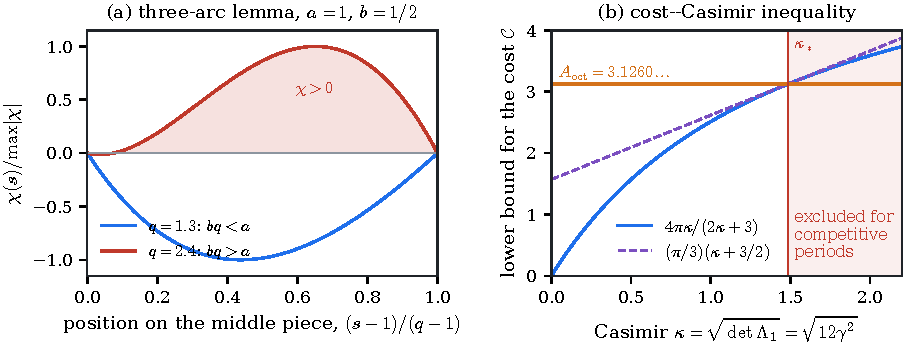
\includegraphics[width=\textwidth]{figures/fig-reverse-estimates.pdf}
  \caption{(a) The obstruction of the three-arc lemma (\cref{lem:three-arc}), growing case, with
  active margin $a=1$ of the middle piece and outer margin $b=a_k=1/2$. The switching function
  of the outer label vanishes at both ends of the middle piece, and its value inside is fixed
  by this. For $q=4/3$ ($bq<a$) it is negative, as the maximum principle requires; for $q=5/2$
  ($bq>a$, that is, $a_ka_{k+2}>a_{k+1}^2$) it becomes positive. The curves are normalized by
  their maximum modulus. (b) The cost--Casimir inequality of \cref{prop:cost-casimir} (solid) and
  the spectral bound of forward periods (dashed), against the octagon's cost $\Aoct$. A
  competitive period has $\kappa<\kappa_*=3\Aoct/(4\pi-2\Aoct)$; the proof of
  \cref{cor:casimir-cap} compares it with $2\sqrt5/3$. Both bounds equal $\pi$ at
  $\kappa=3/2$.}
  \label{fig:reverse-estimates}
\end{figure}

\section{Classes R and M3}\label{sec:reverse}

This section excludes the two classes whose obstruction is local: an entirely reverse period
(class $\cls{R}$) and a mixed period with a maximal reverse run of length other than two (class
$\cls{M3}$). Both exclusions hold for every normal vertex period, whatever its cost and its
number of pieces. They rest on two facts about a few consecutive pieces. Across three reverse
switches the active margin of an interior piece cannot be a minimum of the four
(\cref{lem:reverse-four}). Across two switches that return to the same label, the active margins
are strictly log-concave (\cref{lem:three-arc}). In a run of reverse switches these two facts
leave room for exactly one configuration, a run of two switches around a strict minimum
(\cref{prop:run-structure}). That configuration is the input of the remaining classes. The
section ends with the proof of ellipticity (\cref{prop:ellipticity}), which uses it.

\subsection{The reverse-four principle}\label{sec:rev-four}

Consider four consecutive pieces $k,k+1,k+2,k+3$ with three reverse switches between them, so
that their labels are $i,\,i-1,\,i+1,\,i$. Name the margins at the switch $\tau_{k+1}$ in the label
order $(i,i+1,i-1)$ as $(P,Q,Z)$, and the factors of the two interior pieces as $b=q_{k+1}$ and
$c=q_{k+2}$. Then $P=a_k$ and $Z=a_{k+1}$. Along piece $k+1$ (label $i-1$) the label $i$ grows and
$i+1$ decreases, so at $\tau_{k+2}$
\[
  A:=m_{k+2}(i+1)=\frac{Z+Q}{b}-Z=a_{k+2},\qquad B:=m_{k+2}(i)=(Z+P)\,b-Z,
\]
and along piece $k+2$ (label $i+1$) the label $i$ decreases, so $a_{k+3}=(A+B)/c-A$.

Suppose the third piece is a weak minimum: $a_{k+2}\le a_k,a_{k+1},a_{k+3}$. In these variables
this reads
\begin{equation}\label{eq:rev-min}
  A\le Z,\qquad bA+(b-1)Z\le B,\qquad (2c-1)A\le B.
\end{equation}
The obstruction is a variation of the period: insert short pieces of the two
inactive controls at the two interior switches (the control $i+1$ at $\tau_{k+1}$ and the
control $i$ at $\tau_{k+2}$), and change the logarithms of the factors of the four pieces at
rates chosen so that the end state and the end frame do not move. To first order the normalized
cost $\cost/\sqrt{12}$ then changes by $\frac{Z}{4}N(A,B,Z,b,c)$ times the size of the variation, where
\begin{multline}\label{eq:rev-N}
  N(A,B,Z,b,c)=b(b-1)A\bigl(Ac\,\eta(c)-B\,\zeta(c)\bigr)\\
  +(c-1)\bigl(bA(B+bZ)\,\eta(b)-B(bA+Z)\,\zeta(b)\bigr),
\end{multline}
with $\eta(t)=t-1-\log t$ and $\zeta(t)=t\log t-t+1$, both positive for $t>1$. Under the
minimum hypothesis~\eqref{eq:rev-min} this derivative is negative
(\cref{lem:rev-N}), so the variation lowers the cost, while the maximum principle says that the
inserted controls are not better than the active ones and the variation cannot lower the cost to
first order. We do not construct the variation. Its content is an exact linear identity between
switching functions at the switches (\cref{lem:rev-identities}), and the maximum principle enters
only through the signs of these switching functions.

\begin{lemma}[Sign of the cost derivative]\label{lem:rev-N}
If $b,c>1$, $A,Z>0$ and~\eqref{eq:rev-min} holds, then $N(A,B,Z,b,c)<0$.
\end{lemma}

The proof (\cref{app:rev-N}) rests on the inequality $(2t+1)\,\eta(t)<(t+2)\,\zeta(t)$ for $t>1$,
which is the Pad\'e bound $\log t>3(t^2-1)/(t^2+4t+1)$.

\begin{lemma}[The reverse-four identities]\label{lem:rev-identities}
In the situation above, with $\chi_j(k)$ the switching functions at the switch $\tau_k$
(\cref{def:costate-coordinates}),
\begin{align}
  B(c-1)\,\chi_{i+1}(k+1)+bD\,\chi_i(k+2)&=-\sqrt3\,Z\,N(A,B,Z,b,c),\label{eq:rev-third}\\
  (b-1)B\,\chi_{i-1}(k+3)+cD\,\chi_i(k+2)&=-\sqrt3\,A\,N(Z,B,A,c,b),\label{eq:rev-second}
\end{align}
where $D=A(c-1)+Z(b-1)$.
\end{lemma}

\begin{proof}
Express the costate coordinates at $\tau_{k+2}$ and $\tau_{k+3}$ through those at $\tau_{k+1}$ by
the transport of \cref{lem:costate-transport}(b) over the two interior pieces. The left sides
are then linear in the six coordinates $\alpha_j(k+1),\beta_j(k+1)$, with coefficients rational
in $P,Q,Z,b,c$ and linear in $\log b$, $\log c$. Five linear relations hold among these
coordinates: the switching functions of the active labels vanish at
$\tau_{k+1}$ (labels $i$ and $i-1$), at $\tau_{k+2}$ (label $i+1$) and at $\tau_{k+3}$ (label $i$),
and $\ip{\Lambda_R}{X}=0$ at $\tau_{k+1}$. Each identity is a combination of these five relations
with polynomial coefficients, listed in \cref{app:rev-identities}; after clearing denominators
both sides are the same polynomial in the variables and in $\log b$, $\log c$.
\end{proof}

The coefficients $B(c-1)$ and $bD$ in~\eqref{eq:rev-third} are the weights of the two
inserted pieces in the variation described above, and $N$ is its cost derivative.

\begin{proof}[Proof of \cref{lem:reverse-four}]
(a) The labels $i+1$ at $\tau_{k+1}$ and $i$ at $\tau_{k+2}$ are inactive on both adjacent pieces,
so their switching functions are $\le0$ (\cref{lem:costate-transport}(c)). The weights
$B(c-1)$ and $bD$ are positive, so the left side of~\eqref{eq:rev-third} is $\le0$
and $N(A,B,Z,b,c)\ge0$. The weak minimum at the third piece is~\eqref{eq:rev-min}, and
\cref{lem:rev-N} gives $N<0$.

(b) A weak minimum at the second piece reads $Z\le A$, $cZ+(c-1)A\le B$ and $(2b-1)Z\le B$: these
are the conditions~\eqref{eq:rev-min} with $(A,Z,b,c)$ replaced by $(Z,A,c,b)$, so
$N(Z,B,A,c,b)<0$. The switching functions $\chi_{i-1}(k+3)$ and $\chi_i(k+2)$ are $\le0$, and
\eqref{eq:rev-second} gives the contradiction as before.
\end{proof}

\subsection{Class R}\label{sec:rev-R}

\begin{proof}[Proof of \cref{thm:class-R}]
The active margins are $N$-periodic, so one of them, $a_m$, is a global minimum. Every switch is
reverse, so the four pieces $m-2,\dots,m+1$ have three reverse switches between them, and
$a_m\le a_{m-2},a_{m-1},a_{m+1}$. This contradicts \cref{lem:reverse-four}(a) for $k=m-2$.
\end{proof}

The window may run through the seam, and it may contain the same piece of the period twice when
$N<4$; the twisted indexing of \cref{sec:periods} makes no distinction. The argument uses neither
the cost nor the number of pieces, and \cref{sec:terminal} uses it also for the entirely reverse
words with five pieces.

\subsection{Three pieces with alternating labels}\label{sec:rev-three}

When the switch after piece $k$ is followed by a switch back to the label of piece $k$, the
middle piece is a turn, and its two outer pieces have the same control. The switching function
of that control vanishes at both ends of the middle piece and is $\le0$ in between. This forces
a relation between the three active margins.

\begin{proof}[Proof of \cref{lem:three-arc}]
(b) After a reverse switch the label $i_k$ is the growing label of piece $k+1$, so
$a_{k+2}=(a_{k+1}+a_k)\,q_{k+1}-a_{k+1}>a_k$ by \cref{lem:one-arc}; after a forward switch it is
the decreasing label and $a_{k+2}=(a_{k+1}+a_k)/q_{k+1}-a_{k+1}<a_k$.

(a) Write $a=a_{k+1}$ and $q=q_{k+1}$. Suppose first that the switch $k$ is reverse, so that the
outer label $i=i_k$ is the growing label of the middle piece, with margin $b=a_k$ at its start, and
$a_{k+2}=(a+b)q-a$. Since
\[
  a^2-b\bigl((a+b)q-a\bigr)=(a+b)(a-bq),
\]
the claim is $bq<a$. By \cref{lem:costate-transport} and \cref{app:rev-one-arc}, the switching
function of the label $i$ at the intermediate factor $s\in[1,q]$ is
\begin{gather*}
  \chi_i(s)=2s\Bigl(Y(s-1)+\frac{\sqrt3a}{2}F(s)\Bigr),\\
  F(s)=(a+b)\log s-(a+b)(s-1)+a\frac{(s-1)^2}{s},
\end{gather*}
for a number $Y$. It vanishes at $s=1$ and $s=q$ and is $\le0$ in between. The vanishing at $q$
fixes $Y$, and $\chi_i\le0$ just before $q$ makes the derivative at $q$ nonnegative. Together
these say $(q-1)F'(q)\ge F(q)$, that is,
\[
  (q-1)(2aq-a+bq)\ge(a+b)\,q^2\log q.
\]
If $bq\ge a$, this fails: the right side minus the left side equals
$a\bigl(q^2\log q-(q-1)(2q-1)\bigr)+b\bigl(q^2\log q-q(q-1)\bigr)$; the second bracket is
positive because $q\log q>q-1$; if the first bracket is negative, replace $a$ by the larger
$bq$, which leaves $bq^2\bigl((q+1)\log q-2(q-1)\bigr)>0$. So $bq<a$.

If the switch $k$ is forward, the outer label is the decreasing label of the middle piece, with
margin $c=a_k$, and $a_{k+2}=(a+c)/q-a$. Now $a^2-c\bigl((a+c)/q-a\bigr)=(a+c)(a-c/q)$, and the
claim is $c<aq$. Here $\chi_i(s)=-(2/s)\bigl(Y(1-s^{-1})+\frac{\sqrt3a}{2}h(s)\bigr)$ with
$h(s)=(a+c)\log s-a(s-1)-c(1-s^{-1})$, and $h(1)=h'(1)=0$. The sign at the start of the piece
gives $Y\ge0$. If $aq\le c$, then
\[
  h(q)=(c-aq)\bigl(\log q-(1-q^{-1})\bigr)+a\bigl((q+1)\log q-2(q-1)\bigr)>0,
\]
so $\chi_i(q)<0$, contradicting $\chi_i(q)=0$.
\end{proof}

The proof uses one end of the middle piece in each case: the right end when the outer label grows,
the left end when it decreases. \Cref{fig:reverse-estimates}(a) shows the switching function of
the growing case for an admissible factor and for one with $bq>a$.

\subsection{Reverse runs}\label{sec:rev-runs}

\begin{proof}[Proof of \cref{prop:run-structure}]
The run is preceded by the forward switch $k-1$ and followed by the forward switch $k+L$.

At the entry, the switches $k-1,k$ are forward then reverse, so $a_{k+1}<a_{k-1}$ by
\cref{lem:three-arc}(b), and $i_{k+1}=i_{k-1}$. If $a_k\le a_{k+1}$, then $a_k$ would be at most
both $a_{k-1}$ and $a_{k+1}$, against \cref{lem:three-arc}(a). So $a_{k+1}<a_k$.

At the exit, the switches $k+L-1,k+L$ are reverse then forward, so $a_{k+L-1}<a_{k+L+1}$, and
\cref{lem:three-arc}(a) on the pieces $k+L-1,k+L,k+L+1$ gives $a_{k+L-1}<a_{k+L}$.

If $L=1$, the entry gives $a_{k+1}<a_k$ and the exit $a_k<a_{k+1}$. If $L\ge3$, let $m$ be a
piece of $k,\dots,k+L$ with the smallest active margin. It is not $k$, since $a_{k+1}<a_k$, nor
$k+L$, since $a_{k+L-1}<a_{k+L}$. If $m=k+1$, the pieces $k,\dots,k+3$ have three reverse switches
and the second one is a weak minimum, against \cref{lem:reverse-four}(b). If
$k+2\le m\le k+L-1$, the pieces $m-2,\dots,m+1$ have three reverse switches and the third one is a
weak minimum, against \cref{lem:reverse-four}(a). So $L=2$. The entry and the exit give the first
three inequalities, and \cref{lem:three-arc}(b) at the switches $k+1,k+2$ gives
$a_{k+1}<a_{k+3}$.
\end{proof}

The proof does not use mixedness beyond the existence of the run: a maximal reverse run is
bounded by forward switches by definition, so a period that has one is mixed.

\begin{proof}[Proof of \cref{thm:class-M3}]
This is the first conclusion of \cref{prop:run-structure}.
\end{proof}

In a mixed period every reverse switch therefore belongs to a pattern $+\,-\,-\,+$ of switch
signs, whose middle piece is a centre, and every centre is a strict local minimum of the active
margins. The other classes use these facts through the following corollary.

\begin{corollary}[Mixed periods]\label{cor:rev-mixed}
Let $P$ be a mixed normal vertex period.
\begin{enumerate}[label=\textup{(\alph*)}]
\item Every reverse switch $k$ is the first or the second switch of a pattern of signs
  $+\,-\,-\,+$: either the switches $k-1,k,k+1,k+2$ or the switches $k-2,k-1,k,k+1$ have these
  signs.
\item At a centre $k$, $a_k<a_{k-1}$ and $a_k<a_{k+1}$.
\item Every switch norm satisfies $d_k\ge3/32$.
\end{enumerate}
\end{corollary}

\begin{proof}
(a) and (b) restate \cref{prop:run-structure}. For (c), at a forward switch
$d_k\ge j_k/2\ge3/32$ by \cref{lem:switch-norms}(a). By (a), a reverse switch is the outgoing
switch of a turn (the piece $k$ after the forward switch $k-1$) or the incoming switch of a turn
(the piece $k+1$ before the forward switch $k+1$), and \cref{lem:switch-norms}(b) gives
$d_k\ge3/32$ in both cases.
\end{proof}

\subsection{Proof of ellipticity}\label{sec:rev-ellipticity}

We prove \cref{prop:ellipticity}: a mixed normal vertex period has $\gamma^2>0$. Suppose
$\gamma^2\le0$. The idea is to read the switch vectors $y_n$ of \cref{lem:per-switch-vectors}
projectively, through a coordinate that changes monotonically from one switch to the next.
Because $y_{N+n}=\pm y_n$, the coordinate returns to its value after one period; but at every
centre it strictly increases, and nowhere does it decrease.

\begin{lemma}[Three Gram vectors]\label{lem:rev-three-gram}
Let $S$ be a symmetric $2\times2$ matrix with $\det S\le0$, and let $y,y',y''$ be vectors with
$y^{\mathsf T}Sy$, $y'^{\mathsf T}Sy'$, $y''^{\mathsf T}Sy''$ all positive. Then
$(y^{\mathsf T}Sy')(y^{\mathsf T}Sy'')(y'^{\mathsf T}Sy'')>0$.
\end{lemma}

\begin{proof}
For two vectors, $(y^{\mathsf T}Sy)(y'^{\mathsf T}Sy')-(y^{\mathsf T}Sy')^2=\det S\cdot\det(y,y')^2\le0$.
The Gram determinant of three vectors of the plane vanishes:
$d\,d'\,d''-d\,c^2-d'\,b^2-d''a^2+2abc=0$ in the obvious notation. With the three two-vector
inequalities, $2abc\ge d\,d'\,d''>0$.
\end{proof}

\begin{lemma}[Signs of the cross pairings]\label{lem:rev-cross-signs}
Suppose $\gamma^2\le0$. At a forward same-sign piece $k$, $e_k>0$. At a centre $k$ with
$a_k<a_{k-1}$, $a_k<a_{k+1}$ and $d_{k-1},d_k\ge3/32$, $e_k<0$.
\end{lemma}

\begin{proof}
At a same-sign piece, \cref{lem:stationarity} expresses $e_k$ through $d_{k-1}$, $d_k$ and the
active margins. At a forward same-sign piece both switches are forward, and the lower bounds
$d\ge j/2$ of \cref{lem:switch-norms}(a) give $e_k\ge X_k$ with
\[
  X_k=\frac1{16}\Bigl(-1+2a\Bigl(\frac1{a+p}+\frac1{a+n}\Bigr)-\frac{a^2}{a^2+4}
  +\log\frac{(a+p)(a+n)}{a^2+4}\Bigr),
\]
$a=a_k$, $p=a_{k-1}$, $n=a_{k+1}$. Here the logarithm is $\log q_k>0$ by
\cref{lem:per-factors}, and $a^2/(a^2+4)<2a/(a+p)$ because $ap<4$; so $X_k>-1/16$. On the other
hand $\gamma^2\le0$ and \cref{lem:gram} give $e_k^2\ge d_{k-1}d_k\ge(3/32)^2$, and $3/32>1/16$, so
$e_k\ge3/32>0$. At a centre the switches are reverse, the upper bounds $d\le j/2$ give
$e_k\le X_k$, and now the logarithm is $-\log q_k<0$ and $2a/(a+p)+2a/(a+n)<2$ by the strict
minimum, so $X_k<1/16$ and $e_k\le-3/32$.
\end{proof}

\begin{proof}[Proof of \cref{prop:ellipticity}]
Suppose $\gamma^2\le0$. By \cref{cor:rev-mixed}(c) every $d_n=y_n^{\mathsf T}Sy_n$ is at least
$3/32$. Let $h(v)=y_0^{\mathsf T}Sv$, a nonzero linear form, and let $l$ be the linear form with
$h(u)l(v)-h(v)l(u)=c\det(u,v)$ for a constant $c>0$. By \cref{lem:rev-three-gram} with
$y=y_0$, $h(y_n)h(y_m)\,(y_n^{\mathsf T}Sy_m)>0$ for all $n,m$; in particular $h(y_n)\ne0$, and the
projective coordinate $z_n=l(y_n)/h(y_n)$ is defined, with
\[
  z_{n+1}-z_n=\frac{c\,\det(y_n,y_{n+1})}{h(y_n)\,h(y_{n+1})}.
\]
By \cref{lem:per-switch-vectors}, at a turn $y_{n+1}=-y_n$ and the increment is $0$. At a forward
same-sign piece $\det(y_n,y_{n+1})=1/K_{n+1}>0$ and $y_n^{\mathsf T}Sy_{n+1}=e_{n+1}>0$
(\cref{lem:rev-cross-signs}), so $h(y_n)h(y_{n+1})>0$ and the increment is positive. At a centre
$\det(y_n,y_{n+1})=-1/K_{n+1}<0$ and $e_{n+1}<0$, using the strict minimum and the bounds
$d\ge3/32$ of \cref{cor:rev-mixed}; so $h(y_n)h(y_{n+1})<0$ and the increment is again positive.
A mixed period has a reverse switch, hence a centre (\cref{cor:rev-mixed}(a)), so the increments
over one period sum to a positive number. But $y_N=\pm y_0$ and $z$ depends only on the line of
the vector, so the sum is $z_N-z_0=0$.
\end{proof}

For an entirely forward period every piece is a forward same-sign piece and the same telescoping gives
$\gamma^2>0$.

\subsection{Costate identities for reverse switches}\label{app:reverse-estimates}

This subsection gives the explicit formulas behind \cref{sec:periods,sec:reverse}: the one-piece
costate map, the two reverse-four identities, the sign of the cost derivative $N$, and the
elementary inequalities of the three-arc lemma, the switch norms and the Casimir cap. Each
identity below is an identity of rational functions in the displayed variables and the
logarithms that occur; it is verified by clearing denominators and expanding.

\subsubsection{The one-piece costate map}\label{app:rev-one-arc}

On a piece with active margin $a$, growing margin $b$ and decreasing margin $c$ at its start
(\cref{lem:one-arc}), the inhomogeneous terms of \cref{lem:costate-transport}(b) at the factor
$q$ are
\begin{align*}
  \mathrm{Act}(a,b,c,q)&=\tfrac{\sqrt3a}{2}\bigl((a+c)(1-q^{-1})-(a+b)(q-1)\bigr),\\
  \mathrm{AG}(a,b,q)&=\tfrac{\sqrt3a}{2}\bigl(a(q^2-1)-(a+b)(q^2-q)\bigr),\\
  \mathrm{AD}(a,c,q)&=\tfrac{\sqrt3a}{2}\bigl((a+c)(q^{-1}-q^{-2})-a(1-q^{-2})\bigr),\\
  \mathrm{BG}(a,b,q)&=\sqrt3a\bigl((a+b)\,q\log q-2a(q-1)\bigr),\\
  \mathrm{BD}(a,c,q)&=\sqrt3a\,q^{-1}\bigl(2a(q-1)-(a+c)\log q\bigr).
\end{align*}
The logarithms come from the cost term $-\frac32[J,X]$ of the costate
equation, integrated against the exponentially moving margins.

These formulas give the switching functions of the two inactive labels inside the piece. Let
$i$ be the active label, and at the start of the piece let $Y=\alpha_i+\alpha_{i+1}$,
$Y'=\alpha_i+\alpha_{i-1}$, $B=\beta_i+\beta_{i+1}$, $B'=\beta_i+\beta_{i-1}$. Since $\chi_i=0$ on
the piece, at the intermediate factor $s\in[1,q]$
\[
  \chi_{i+1}(s)=2s^2Y+sB+\sqrt3\,a\,s\,F(s),\qquad
  \chi_{i-1}(s)=\frac{2Y'}{s^2}+\frac{B'}{s}-\frac{\sqrt3\,a}{s}\,h(s),
\]
where
\begin{align*}
  F(s)&=(a+b)\log s-(a+b)(s-1)+a\,\frac{(s-1)^2}{s},\\
  h(s)&=(a+c)\log s-a(s-1)-c\,(1-s^{-1}),
\end{align*}
because $2\mathrm{AG}+\mathrm{BG}=\sqrt3asF$ and $2\mathrm{AD}+\mathrm{BD}=-\sqrt3a\,h/s$. Both $F$ and
$h$ vanish to second order at $s=1$: $F(1)=F'(1)=h(1)=h'(1)=0$. When the growing label was active
on the previous piece, $\chi_{i+1}(1)=2Y+B=0$ and
\[
  \chi_{i+1}(s)=2s\Bigl(Y(s-1)+\frac{\sqrt3a}{2}F(s)\Bigr);
\]
when the decreasing label was, $B'=-2Y'$ and
\[
  \chi_{i-1}(s)=-\frac2s\Bigl(Y'(1-s^{-1})+\frac{\sqrt3a}{2}h(s)\Bigr).
\]
These are the forms used in \cref{lem:switch-norms}(a) and in \cref{lem:three-arc}. In each case the derivative at $s=1$ is $\pm2Y$ or $\pm2Y'$, which is how
the sign condition at the start of a piece fixes the sign of $Y$ or $Y'$.

\subsubsection{The reverse-four identities}\label{app:rev-identities}

In the notation of \cref{sec:rev-four}, let $x_j,y_j$ be the coordinates $\alpha,\beta$ at the
switch $\tau_{k+1}$ in the label order $(i,i+1,i-1)$, so that $j=0,1,2$ stands for the labels
$i,i+1,i-1$, and let $u_j,v_j$ and $r_j,s_j$ be those at $\tau_{k+2}$ and $\tau_{k+3}$ in the same
order. The transport over piece $k+1$ (active margin $Z$, growing margin $P$, decreasing margin
$Q$, factor $b$) and over piece $k+2$ (active margin $A$, growing margin $Z$, decreasing margin
$B$, factor $c$) gives
\begin{align*}
  u_2&=x_2+\mathrm{Act}(Z,P,Q,b),\\
  u_0&=b^2(x_2+x_0)+\mathrm{AG}(Z,P,b)-u_2,\\
  u_1&=b^{-2}(x_2+x_1)+\mathrm{AD}(Z,Q,b)-u_2,\\
  r_1&=u_1+\mathrm{Act}(A,Z,B,c),\\
  r_0&=c^{-2}(u_1+u_0)+\mathrm{AD}(A,B,c)-r_1,\\
  r_2&=c^2(u_1+u_2)+\mathrm{AG}(A,Z,c)-r_1,
\end{align*}
and the same with $(\alpha,\mathrm{Act},\mathrm{AG},\mathrm{AD})$ replaced by
$(\beta,-2\mathrm{Act},\mathrm{BG},\mathrm{BD})$ and the powers $b^{\pm2},c^{\pm2}$ by
$b^{\pm1},c^{\pm1}$. The five relations are
\begin{gather*}
  h_1=2x_0+y_0,\quad h_2=2x_2+y_2,\quad h_3=2u_1+v_1,\quad h_4=2r_0+s_0,\\
  h_5=y_0(Q+Z)+y_1(P+Z)+y_2(P+Q),
\end{gather*}
all equal to $0$: the active switching functions at the three switches, and
$\ip{\Lambda_R}{X}=0$ at $\tau_{k+1}$. Then, with $D=A(c-1)+Z(b-1)$ and as identities in all the
variables,
\begin{align*}
  B(c-1)&(2x_1+y_1)+bD(2u_0+v_0)+\sqrt3ZN(A,B,Z,b,c)\\
  &=b^2(c-1)(Q-Zb+Z)\,h_1+(b^2-1)(c-1)(Pb+Q)\,h_2\\
  &\quad+b(c-1)(Pb^2+Zb^2+Zbc-Zc-Z)\,h_3+Zbc^2(b-1)\,h_4\\
  &\quad-b(b-1)(c-1)\,h_5,
\end{align*}
and
\begin{align*}
  (b-1)&B(2r_2+s_2)+cD(2u_0+v_0)+\sqrt3AN(Z,B,A,c,b)\\
  &=bc(c-1)(Q-Zb+Z)\,h_1\\
  &\quad+\tfrac{c(b-1)}{b}\bigl(Pb^2c+Qbc-Qb+Qc-Q+Zb^2-Zbc+Zc-Z\bigr)\,h_2\\
  &\quad+(b-1)(c^2-1)(Pb+Zb+Zc-Z)\,h_3+Zc^3(b-1)\,h_4\\
  &\quad-c(b-1)(c-1)\,h_5,
\end{align*}
with $A=(Z+Q)/b-Z$ and $B=(Z+P)b-Z$. Setting the five
relations to zero gives \cref{lem:rev-identities}.

\subsubsection{The sign of the cost derivative}\label{app:rev-N}

Let $\eta(t)=t-1-\log t$ and $\zeta(t)=t\log t-t+1$. For $t>1$ both are positive.

\begin{lemma}[Pad\'e bound]\label{lem:rev-pade}
For $t>1$, $3(t^2-1)<(t^2+4t+1)\log t$; equivalently $(2t+1)\,\eta(t)<(t+2)\,\zeta(t)$. In
particular $\eta(t)<\zeta(t)$.
\end{lemma}

\begin{proof}
The function $\psi(t)=\log t-3(t^2-1)/(t^2+4t+1)$ vanishes at $1$ and
$\psi'(t)=(t-1)^4/\bigl(t(t^2+4t+1)^2\bigr)>0$ for $t>1$. The second form follows from
$(t+2)\zeta(t)-(2t+1)\eta(t)=(t^2+4t+1)\log t-3(t^2-1)$, and the third because $(2t+1)/(t+2)>1$
and $\eta(t)>0$.
\end{proof}

\begin{proof}[Proof of \cref{lem:rev-N}]
Recall~\eqref{eq:rev-N} and the hypotheses $b,c>1$, $A,Z>0$, $A\le Z$, $bA+(b-1)Z\le B$ and
$(2c-1)A\le B$. In particular $B>cA>0$.

The first bracket of $N$ is negative: $Ac\,\eta(c)<Ac\,\zeta(c)<B\,\zeta(c)$.

The second bracket, $T(B)=bA(B+bZ)\,\eta(b)-B(bA+Z)\,\zeta(b)$, is affine in $B$ with slope
$bA\,\eta(b)-(bA+Z)\,\zeta(b)<0$, so $T(B)\le T(B_0)$ with $B_0=bA+(b-1)Z$. At $B_0$ we have
$B_0+bZ=bA+(2b-1)Z$ and $B_0(bA+Z)=b^2A^2+b^2AZ+(b-1)Z^2>0$, and \cref{lem:rev-pade} at $t=b$ gives
\begin{align*}
  (b+2)\,T(B_0)&<\eta(b)\bigl[(b+2)\,bA\bigl(bA+(2b-1)Z\bigr)\\
  &\qquad\qquad-(2b+1)\bigl(b^2A^2+b^2AZ+(b-1)Z^2\bigr)\bigr]\\
  &=-(b-1)\,\eta(b)\bigl(b^2A^2+2bZ(Z-A)+Z^2\bigr),
\end{align*}
which is $\le0$ because $Z\ge A$. So $T(B)<0$, and
$N=b(b-1)A\cdot(\text{first bracket})+(c-1)\,T(B)<0$.
\end{proof}

\subsubsection{Elementary inequalities}\label{app:rev-elementary}

\runin{Logarithms.} For $q>1$, $2(q-1)<(q+1)\log q$ and $q-1<q\log q$: both differences vanish
at $q=1$, with derivatives
$\log q+q^{-1}-1>0$ and $\log q>0$. They give the signs in the proof of \cref{lem:three-arc}.

\runin{The turn secant.} With $f(x)=x-x^{-1}-\log x$,
\[
  f'(x)-\tfrac34=\frac{(x-2)^2}{4x^2},\qquad 1-f'(x)=\frac{x-1}{x^2}.
\]
So every secant slope of $f$ on $(1,\infty)$ lies in $[3/4,1)$, and the switch norm at a turn,
$d=\frac18\times$(secant slope), satisfies $3/32\le d<1/8$. At a forward switch the lower bound
$d_k\ge3/32$ comes instead from
$j_k/2-3/32=(a_k-a_{k+1})^2/(32s_k^2)\ge0$.

\runin{The cross pairing bound.} With $a,p,n>0$ and $j(a,b)=(a^2+ab+b^2)/(4(a+b)^2)$,
\begin{multline*}
  \frac{1}{2a}\Bigl((a+p)\,\frac{j(p,a)}{2}+(a+n)\,\frac{j(a,n)}{2}
  -\frac{G_a(a,p)+G_a(a,n)}{16}\Bigr)\\
  =\frac{1}{16}\Bigl(-1+\frac{2a}{a+p}+\frac{2a}{a+n}-\frac{a^2}{a^2+4}
  +\log\frac{(a+p)(a+n)}{a^2+4}\Bigr).
\end{multline*}
This is the quantity $X_k$ of \cref{lem:rev-cross-signs}: by
\cref{lem:stationarity}, at a same-sign piece $e_k$ is an increasing affine function of
$d_{k-1}$ and $d_k$, and $X_k$ is its value at $d=j/2$.

\begin{lemma}[Octagon cost comparison]\label{lem:octagon-cost-comparison}
The octagon cost satisfies
\[
 \frac{\Aoct}{\pi}<\frac{203}{204}<\frac{8\sqrt5}{9+4\sqrt5},\qquad
 \Aoct<\frac{161\pi}{162}+\frac{9\sqrt3}{4000}.
\]
\end{lemma}

\begin{proof}
We use positive integral remainders in the exact formula for $\Aoct$.
Set $s=\sin(\pi/12)=(\sqrt6-\sqrt2)/4$ and put
\[
 P=12s\left(1+\frac{s^2}{6}+\frac{3s^4}{40}+\frac{5s^6}{112}\right),\qquad
 L=2\sum_{j=0}^{4}\frac{1}{(2j+1)3^{2j+1}}.
\]
The fourth derivative of $(1-x)^{-1/2}$ is positive on $[0,1)$.
Its cubic Taylor polynomial at zero therefore gives
\[
 \pi=12\int_0^s\frac{\dd t}{\sqrt{1-t^2}}
 >12\int_0^s\left(1+\frac{t^2}{2}+\frac{3t^4}{8}+\frac{5t^6}{16}\right)\dd t=P.
\]
Similarly, the geometric remainder gives
\[
 \log2=2\int_0^{1/3}\frac{\dd t}{1-t^2}
 >2\int_0^{1/3}\sum_{j=0}^4t^{2j}\,\dd t=L.
\]
Thus
\[
 \Aoct<U:=\frac{\sqrt{12}(8-4\sqrt2-L)}{2\sqrt2-1}.
\]
We compare $U$ directly with $qP+b\sqrt3$, for the two pairs
\[
 (q,b)\in\left\{\left(\frac{203}{204},0\right),
                       \left(\frac{161}{162},\frac9{4000}\right)\right\}.
\]
Write
\[
 \begin{gathered}
 m=1+\frac1{12}+\frac{21}{640}+\frac{65}{3584},\qquad
 n=\frac1{24}+\frac3{160}+\frac{75}{7168},\\
 p=3(m+n),\qquad r=3(m+3n).
 \end{gathered}
\]
The bracket in $P$ expands to $m-n\sqrt3$, so $P=p\sqrt6-r\sqrt2$.
With
\[
 A=4qp-16+2L-b,\qquad B=8-qp+2b,\qquad C=qr,
\]
we have
\[
 (qP+b\sqrt3-U)(2\sqrt2-1)=(A+B\sqrt2)\sqrt3-C(4-\sqrt2).
\]
For each pair, direct rational substitution gives $B>0$, $A+B>0$, $C>0$ and
\[
 \begin{gathered}
 R:=18C^2-3A^2-6B^2>0,\qquad T:=6AB+8C^2>0,\\
 2T^2-R^2>0.
 \end{gathered}
\]
The quantities $(A+B\sqrt2)\sqrt3$ and $C(4-\sqrt2)$ are positive.
Their squared difference is $T\sqrt2-R>0$, proving $U<qP+b\sqrt3$.
Since $q>0$ and $P<\pi$, both cost bounds follow.
Finally, $\lambda=\sqrt5-2=1/(\sqrt5+2)<1/4$ gives
\[
 \frac{8\sqrt5}{9+4\sqrt5}=1-\lambda^4
 >1-4^{-4}>\frac{203}{204}.
\]
\end{proof}

\section{Class M1: every forward run short}\label{sec:short-runs}

A period of class \cls{M1} is mixed, every maximal run of reverse switches has length two and
every maximal run of forward switches has length one (\cref{def:classes}). Its cyclic sign word is
therefore $(--+)^m$: every reverse run is a pair of reverse switches around a centre piece, and
consecutive pairs are separated by single forward switches. This section proves \cref{thm:class-M1}.



The theorem uses neither the compact domain nor a lower bound on the number of pieces. Its proof
compares two ways of counting how far the switch vectors $y_k$ of \cref{def:normal-multiplier}
turn in one period, measured in the positive definite form $S$. At a turn the switch vector only
changes sign, so all the turning happens at the $m$ centres. A whole-period winding identity fixes
the total turning at exactly $(m+1)\pi/3$, because the frame of a competitive period turns by
exactly $\pi/3$. A local estimate at each centre, which combines the stationarity identity, the
Gram identity and the competitive cap on the Casimir $\gamma^2$, shows that each centre turns the
switch vectors by more than $2\pi/5$. The average $(m+1)\pi/(3m)$ is at most $2\pi/5$ as soon as
$m\ge5$, and the word condition leaves $m=2$ as the only other case. With two centres the
recurrence of the switch vectors closes up only in a rigid configuration whose cost can be computed
exactly, and it exceeds $\Aoct$.

\subsection{The sign word}

\begin{lemma}\label{lem:m1-pattern}
  Let a vertex representation with $N$ pieces belong to class \cls{M1}. Then $N=3m$ for an integer
  $m\ge1$ with $m\equiv2\pmod 3$, and there is $k_0\in\Z$ such that for every $j\in\Z$ the
  switches $k_0+3j$ and $k_0+3j+1$ are reverse and the switch $k_0+3j+2$ is forward.
\end{lemma}

\begin{proof}
  A mixed representation has a forward switch followed by a reverse one: otherwise every switch
  after the first forward one would be forward, which the periodicity $\varepsilon_{k+N}=\varepsilon_k$
  of the signs forbids. Start at such a pair. The reverse run that begins there has length two,
  and the forward run that follows it has length one, so the signs continue as
  $-,-,+,-,-,+,\dots$ with period three. Hence $N=3m$ and the word is $(--+)^m$. The signs of one
  period add up to $m-2m=-m$, and \cref{lem:sign-sum} gives $-m\equiv1\pmod3$.
\end{proof}

We fix $k_0$ and $m$ as in the lemma and call the piece $c_j=k_0+3j+1$, which lies between the two
reverse switches of the $j$-th run, the $j$-th \emph{centre}. The pieces $c_j+1$ and $c_j+2$ are
turns: one of their two switches is forward and the other reverse. At a turn the outgoing switch
vector is the negative of the incoming one, so the three switch vectors that follow the centre
$c_j$ are $z_j$, $-z_j$, $z_j$ with $z_j=y_{c_j}$. Between two consecutive centres the switch
vectors therefore do not turn, and the whole turning of the sequence $(y_k)$ is concentrated at
the centres.

\subsection{The data at a centre}

Fix a centre $c$, with active margin $a=a_c$ and neighbouring active margins $p=a_{c-1}$ and
$n=a_{c+1}$. In this section we write
\begin{equation}\label{eq:m1-variables}
  \begin{gathered}
    r=\frac a{a+p},\qquad t=\frac a{a+n},\qquad \rho=\frac{a^2}{a^2+4},\\
    u=8d_{c-1},\qquad v=8d_c,\qquad E=16e_c,\qquad U(s)=1-s+s^2.
  \end{gathered}
\end{equation}
Here $d_{c-1}$ and $d_c$ are the switch norms of the two reverse switches at the ends of the
centre and $e_c$ is the cross pairing on the centre. The letter $\rho$ is local to this section.

\begin{lemma}\label{lem:m1-centre-data}
  Let $P$ be a normal vertex period with the sign word of \cref{lem:m1-pattern}, and let $\gamma^2$
  be its Casimir. At every centre the numbers \eqref{eq:m1-variables} satisfy
  \begin{enumerate}[label=\textup{(\roman*)}]
    \item $0<r<\tfrac12$, $0<t<\tfrac12$ and $0<\rho<rt$;
    \item $\tfrac34\le u\le U(r)$ and $\tfrac34\le v\le U(t)$;
    \item the stationarity identity
    \begin{equation}\label{eq:m1-stat}
      E=1+r+t-\rho+\log\frac{\rho}{rt}-\frac{1-u}r-\frac{1-v}t;
    \end{equation}
    \item the Gram identity $16(1-\rho)^2\gamma^2=4uv-E^2$.
  \end{enumerate}
\end{lemma}

\begin{proof}
  (i) The centre is the middle piece of a reverse run of length two, so its active margin is
  strictly smaller than both neighbouring ones (\cref{prop:run-structure}). This gives
  $r,t<1/2$. The factor of the centre is $q_c=(a^2+4)/((a+p)(a+n))$, and $q_c>1$ is the
  inequality $(a+p)(a+n)<a^2+4$, which is $\rho<rt$.

  (ii) Both neighbours of the centre are turns. The switch norms at the two ends of a turn are
  equal and at least $3/32$ (\cref{lem:switch-norms}); this gives $u,v\ge 3/4$. Both switches of
  the centre are reverse, so $d_{c-1}\le j_{c-1}/2$ and $d_c\le j_c/2$ by \cref{lem:switch-norms},
  and $4j_{c-1}=(a^2+ap+p^2)/(a+p)^2=U(r)$, and likewise $4j_c=U(t)$.

  (iii) is the stationarity identity of \cref{lem:stationarity} with both incident signs equal to
  $-1$, written in the variables \eqref{eq:m1-variables}.

  (iv) is the Gram identity $d_{c-1}d_c-e_c^2=\gamma^2/(a^2+4)^2$ at a centre (\cref{lem:gram}),
  multiplied by $256$, since $1-\rho=4/(a^2+4)$.
\end{proof}

Since the period is mixed, $\gamma^2>0$ (\cref{prop:ellipticity}), and the switch norms are
positive. The form $S$, whose determinant is $\gamma^2$, is then positive definite, and the number
\[
  \cos\varphi_c=\frac{e_c}{\sqrt{d_{c-1}d_c}}=\frac{E}{2\sqrt{uv}}
\]
is the cosine of the angle $\varphi_c\in(0,\pi)$ between $y_{c-1}$ and $y_c$ in the inner product
$S$; by (iv) its absolute value is less than one. The determinant $\det(y_{c-1},y_c)=-1/(a^2+4)$
is negative at every centre, so all the centres turn the switch vectors in the same sense. We call
$\varphi_c$ the \emph{centre angle}.

\subsection{The angle gap}

A centre with a large angle cosine needs a large pairing $E$. The stationarity identity
\eqref{eq:m1-stat} allows a large $E$ only when $\log(\rho/(rt))$ is not too negative, that is,
when the centre margin is not too small compared with its neighbours. A large centre margin makes
the factor $16(1-\rho)^2$ in the Gram identity (iv) small, and then (iv) forces the Casimir
$\gamma^2$ up, against the competitive cap of \cref{cor:casimir-cap}. The next proposition makes
the conflict quantitative.

\begin{proposition}\label{prop:m1-angle-gap}
  Let $\gamma^2,r,t,\rho,u,v,E$ be real numbers satisfying \textup{(i)--(iv)} of
  \cref{lem:m1-centre-data}, and suppose that $\gamma^2\le 5/27$. Then
  $E<\frac35\sqrt{uv}$; that is, $\cos\varphi<3/10$ for $\cos\varphi=E/(2\sqrt{uv})$.
\end{proposition}

The proof, in \cref{app:short-run-estimates}, reduces the seven variables to two in three steps.
Write $E=(1-\rho+\log\rho)+\Psi(r,u)+\Psi(t,v)$ with $\Psi(r,u)=r-\log r-(1-u)/r$, and let
$\omega(x)=-x-\log(1-x)=\sum_{n\ge2}x^n/n$ for $0\le x<1$.
\begin{enumerate}[label=(\alph*)]
  \item One reverse switch at a time: for $s=\sqrt{4u-3}$ one has $u=U((1-s)/2)$, $2r\le 1-s$, and
  $\Psi(r,u)\le\omega(s)+\log2$, with equality when $r=(1-s)/2$, that is, when the switch bound
  $u\le U(r)$ is attained.
  \item The two switches together: define $S\ge0$ by $S^2=s^2+s'^2+s^2s'^2/3$, where
  $s'=\sqrt{4v-3}$. Then $uv=3(3+S^2)/16$, and $\omega(s)+\omega(s')\le\omega(S)$ because
  $\omega$ is superadditive in $x^2$.
  \item The centre: $z=4\rho/(1-S)$ lies in $(0,1]$, $\rho=(1-S)z/4$, and
  $E\le(1-S)(1-z/4)+\log z$.
\end{enumerate}
If $\cos\varphi\ge3/10$, then $E^2\ge\frac{9}{25}uv$, and the symmetric minimum proved in
\cref{lem:m1-core} gives $16K_*(1-\rho)^2<4uv-E^2$ for the cap $K_*=5/27$, which
contradicts (iv). \Cref{fig:short-runs-gap} shows the region of $(S,z)$ that survives the
reductions and the least Casimir compatible with it.

\begin{figure}[htbp]
  \centering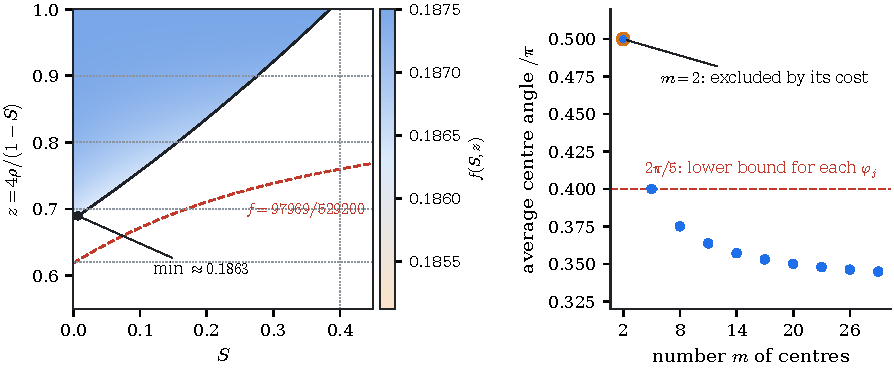
\includegraphics[width=\textwidth]{figures/fig-short-runs-gap.pdf}
  \caption{Left: the pairing constraint $E_{\max}\ge\frac35\sqrt{uv}$ in the reduced
  $(S,z)$ variables, with $E_{\max}$ the envelope in (c). The colour shows the Gram lower bound
  $(4uv-E_{\max}^2)/(16(1-\rho)^2)$. Its minimum occurs on the boundary at $S=0$
  (\cref{lem:m1-symmetric}); the dashed level $5/27$ lies outside the feasible region.
  Right: the average centre angle $(m+1)\pi/(3m)$ forced by winding, for $m\equiv2\pmod3$,
  against the lower bound $2\pi/5$ for every centre. They meet at $m=5$; only $m=2$
  lies above the line.}\label{fig:short-runs-gap}
\end{figure}

\begin{corollary}\label{cor:m1-angle}
  At every centre of a competitive normal vertex period of class \cls{M1}, $\varphi_c>2\pi/5$.
\end{corollary}

\begin{proof}
  The Casimir and the first switch norm are positive, so the competitive cap in
  \cref{cor:casimir-cap} gives $\gamma^2<5/27$. By \cref{lem:m1-centre-data} and
  \cref{prop:m1-angle-gap}, $\cos\varphi_c<3/10$. Since $\cos(2\pi/5)=(\sqrt5-1)/4>3/10$, which
  is $\sqrt5>11/5$, and the arccosine decreases, $\varphi_c>2\pi/5$.
\end{proof}

\subsection{The winding identity}

\begin{proposition}\label{prop:m1-winding}
  Let $P$ be a competitive normal vertex period with the sign word of \cref{lem:m1-pattern}, $N=3m$,
  and positive Casimir. Then
  \[
    \sum_{j=0}^{m-1}\varphi_{c_j}=\frac{(m+1)\pi}3,\qquad
    \varphi_c=\arccos\frac{E_c}{2\sqrt{u_cv_c}},
  \]
  where $E_c,u_c,v_c$ are the numbers \eqref{eq:m1-variables} at the centre $c$.
\end{proposition}

The identity says that the switch vectors, which turn only at the centres, turn in total by the
angle that the frame of the period prescribes. The proof expresses the switch vectors through the
physical frame and follows a continuous angle along the period.

\runin{Switch vectors in the physical frame.} Let $V(t)=g(t)X(t)$ be the tangent frame. The
switch vector at the switch $n$ is, up to a sign and a positive factor, $KV(\tau_n)b$, where
$K=R^{i_0}C(-X(0))$ is a fixed matrix with $\det K=-2\sqrt3$, $C$ is the triangular change of
coordinates, and $b$ is one of two base vectors $b_{\mathrm{in}}(i)$ and
$b_{\mathrm{out}}(i)=Rb_{\mathrm{in}}(i)$ that depend only on the label $i$ of the piece. Factor
$S=Q^{\mathsf T}Q$ with $\det Q<0$, so that angles for $S$ become Euclidean angles after $Q$.

\runin{A continuous angle.} The polar number $z(g)=(g_{00}+g_{11})/2+i(g_{10}-g_{01})/2$ of a
matrix of determinant one has modulus at least one, and for every vector $w\ne0$ the quotient
$gw/(z(g)w)$ lies in the right half-plane, since
$\operatorname{Re}\bigl(gw\cdot\overline{z(g)w}\bigr)=(\abs{gw}^2+\abs{w}^2)/2$. Let $\Phi(t)$ be a
continuous angle of $z(g(t))$. For $w\ne0$ let $\kappa_t(w)$ be the angle from $w$ to
$QKg(t)X(t)w$ obtained by adding $\Phi(t)$ to principal arguments that never leave the slit
plane; it depends continuously on $t$.

\runin{Three facts.} At a centre $c$ the centre angle is
$\varphi_c=\pi/3+\kappa_{\tau_c}(b_{\mathrm{out}})-\kappa_{\tau_c}(b_{\mathrm{in}})$. Along a piece
the base vector that is being followed is an eigenvector of the tangent factor of the piece, so
$g(t)X(t)b$ keeps its direction and $\kappa_t(b)$ is constant; between consecutive centres the
outgoing base vector of one is, up to sign, the incoming base vector of the next. Across the
seam, $\kappa_T(w)=\kappa_0(Rw)+\pi/3$, because $g(0)=I$, $g(T)=R$ and $\Phi(T)-\Phi(0)=\pi/3$.

\runin{The frame turns by exactly $\pi/3$.} The endpoint conditions fix $\Phi(T)-\Phi(0)$ only
modulo $2\pi$. For a competitive period the cost is at most $\Aoct<\pi$, and the winding theorem
behind the reverse comparison (\cref{prop:reverse-comparison}) shows that the reflected first row
$(g_{00},-g_{01})$ of the frame turns by exactly $\pi/3$. The real part of the product of that row
with the conjugate of $z(g)$ is $(g_{00}^2+g_{01}^2+1)/2>0$, so the two angles stay within $\pi/2$
of each other, and $\Phi(T)-\Phi(0)=\pi/3$.

\runin{Telescoping.} The centre angles are periodic in $j$ with period $m$, so we may take the $m$
centres of one period in a window that starts at the seam. Summing the centre formula over them,
the term $\kappa(b_{\mathrm{out}})$ of each centre cancels the term $\kappa(b_{\mathrm{in}})$ of
the next, and the last link crosses the seam, where it gains $\pi/3$. What remains is
$m\cdot\pi/3+\pi/3$.

\subsection{Five or more centres}

\begin{proof}[Proof of \cref{thm:class-M1} for $m\ge5$]
  By \cref{cor:m1-angle} every centre angle exceeds $2\pi/5$, so the sum in
  \cref{prop:m1-winding} exceeds $2m\pi/5$. For $m\ge5$, $2m/5\ge(m+1)/3$, which contradicts
  \cref{prop:m1-winding}. Since $m\equiv2\pmod3$, the only other case is $m=2$.
\end{proof}

\subsection{Two centres}

For $m=2$ the average centre angle is $\pi/2>2\pi/5$, and the angle count gives nothing. The
argument uses instead the recurrence of the switch vectors and the cost identity. For the centre
$c_j$ put $K_j=a_{c_j}^2+4$, write $b_j=a_{c_j+1}$ and $b'_j=a_{c_j+2}$ for the active margins of
the two turns that follow it, and
\[
  D_j=(a_{c_j}+b_j)^2+(b'_j+a_{c_{j+1}})^2-(b_j+b'_j)^2=s_{c_j}^2+s_{c_j+2}^2-s_{c_j+1}^2 .
\]

\begin{lemma}\label{lem:m1-recurrence}
  In a normal vertex period with the sign word of \cref{lem:m1-pattern}, the vectors $z_j=y_{c_j}$
  satisfy
  \[
    K_{j+1}z_{j+1}=-K_jz_{j-1}+D_jz_j,\qquad \det(z_{j-1},z_j)=-1/K_j,
  \]
  and the cyclic product of the period is $\pm I$, so that $z_{j+m}=\pm z_j$ with one sign for all
  $j$.
\end{lemma}

\begin{proof}
  Work in triangular coordinates and in the frame of the centre $c=c_j$, that is, multiply all
  vectors by the inverse of the prefix product up to $c$. Put $A_\pm(q)=T_0(q)R^{\mp1}$, so that
  \[
    A_+(q)=\begin{pmatrix}q&-q\\ 1/q&0\end{pmatrix},\qquad
    A_-(q)=\begin{pmatrix}0&q\\ -1/q&1/q\end{pmatrix},
  \]
  and write $K=K_j$ and $s_k=a_k+a_{k+1}$. The factors of the centre and of the two turns after it
  are $K/(s_{c-1}s_c)$, $s_{c+1}/s_c$ and $s_{c+1}/s_{c+2}$. In this frame
  $z_{j-1}=-(1/s_{c-1},0)^{\mathsf T}$ and $z_j=(0,s_{c-1}/K)^{\mathsf T}$, which gives the
  determinant, and
  \begin{align*}
    K_{j+1}z_{j+1}
    &=s_{c+2}\,A_-\Bigl(\frac K{s_{c-1}s_c}\Bigr)A_+\Bigl(\frac{s_{c+1}}{s_c}\Bigr)
      A_-\Bigl(\frac{s_{c+1}}{s_{c+2}}\Bigr)\begin{pmatrix}0\\1\end{pmatrix}
    =\begin{pmatrix}K/s_{c-1}\\ (s_{c-1}/K)\,D_j\end{pmatrix}\\
    &=-Kz_{j-1}+D_jz_j .
  \end{align*}
  Multiplying back by the prefix product preserves the recurrence and the determinant. The
  cyclic product of the period is $\pm I$ by the tangent closure (\cref{lem:tangent-closure}).
\end{proof}

\begin{lemma}\label{lem:m1-euler}
  For every normal vertex period,
  \[
    \frac{2\cost}{\sqrt{12}}
    =8\sum_{k=0}^{N-1}(\varepsilon_{k-1}+\varepsilon_k)e_k
      -2\sum_{k=0}^{N-1}\frac{\varepsilon_{k-1}+\varepsilon_k}{a_k^2+4}.
  \]
\end{lemma}

\begin{proof}
  Multiply the stationarity identity of \cref{lem:stationarity} at the piece $k$ by $a_k$ and sum
  over a period. The switch norms and the cross pairings are formed from one weight $w_k$ per piece,
  $d_k=(w_k+w_{k+1})/(2s_k^2)$ and $e_k=w_k/(2(a_k^2+4))$. Regrouped by switches, the left-hand
  sides add up to $\sum_k(\varepsilon_{k-1}+\varepsilon_k)w_k\bigl(1-a_k^2/(a_k^2+4)\bigr)
  =8\sum_k(\varepsilon_{k-1}+\varepsilon_k)e_k$. On the right-hand side, the one-arc cost formula
  of \cref{lem:one-arc}, with the factors written in the active margins, gives
  $8\cost/\sqrt{12}=\sum_k\varepsilon_kG(a_k,a_{k+1})$ for the signed action
  \[
    G(a,b)=3ab-4-(a^2+b^2)\log(a+b)+\tfrac12a^2\log(a^2+4)+\tfrac12b^2\log(b^2+4),
  \]
  and the stationarity identity involves the partial derivatives of $G$. The Euler-type identity
  $aG_a(a,b)+bG_b(a,b)=2G(a,b)+16/(a^2+4)+16/(b^2+4)$ turns the sum of the right-hand sides into
  $2\cost/\sqrt{12}+2\sum_k(\varepsilon_{k-1}+\varepsilon_k)/(a_k^2+4)$.
\end{proof}

In the word $(--+)^m$, $\varepsilon_{k-1}+\varepsilon_k$ is $-2$ at a centre and $0$ at a turn,
so the lemma reads $\cost/\sqrt{12}=2\sum_j1/K_j-8\sum_je_{c_j}$.

\begin{proposition}\label{prop:m1-two-centre}
  A competitive normal vertex period with $N=6$ does not have the sign word $(--+)^2$.
\end{proposition}

\begin{proof}
  The two recurrences of \cref{lem:m1-recurrence} read $K_1z_1=-K_0z_{-1}+D_0z_0$ and
  $K_0z_2=-K_1z_0+D_1z_1$, with $z_{-1}=\pm z_1$ and $z_2=\pm z_0$, and $z_0,z_1$ are independent.
  The sign $+$ would give $(K_0+K_1)z_1=D_0z_0$, which is impossible. So $z_{-1}=-z_1$, and the
  recurrences give $K_0=K_1$ and $D_0=D_1=0$. Hence both centres have the same active margin $a$,
  $K=a^2+4$, and $e_{c_0}=z_{-1}^{\mathsf T}Sz_0=-e_{c_1}$. \Cref{lem:m1-euler} gives the exact
  cost
  \[
    \cost=\sqrt{12}\cdot\frac 4K=\frac{8\sqrt3}{a^2+4}.
  \]
  It remains to bound $a$ from above. The equation $D_j=0$ is $(b_j-a)(b'_j-a)=2a^2$, and the
  turn margins exceed $a$ by \cref{prop:run-structure}. By \cref{lem:m1-bc},
  $b_jb'_j\ge(1+\sqrt2)^2a^2$ and $(a+b_j)(a+b'_j)=2b_jb'_j$. The two centre factors exceed one,
  that is, $(a+b'_1)(a+b_0)<K$ and $(a+b'_0)(a+b_1)<K$. Multiplying,
  $K^2>4\,b_0b'_0\,b_1b'_1\ge4(1+\sqrt2)^4a^4$, so
  $K>2(1+\sqrt2)^2a^2$ and $a^2<4/(5+4\sqrt2)$. Consequently
  \[
    \cost>\frac{8\sqrt3}{4+4/(5+4\sqrt2)}=\sqrt3(2\sqrt2-1).
  \]
  This lower bound exceeds $\Aoct$. Indeed, with $r=\sqrt2$, the midpoint inequality for
  $x\mapsto1/x$ on $[1,r]$ gives $\log2>4(r-1)/(r+1)=12-8r$, and hence
  \[
   (2r-1)\Bigl(\frac{2r-1}{2}-\doct\Bigr)
   =\log2+2r-\frac72>\frac{17}{2}-6r=\frac{(3-2r)^2}{2}>0.
  \]
  Since $\Aoct=2\sqrt3\,\doct$, the period is not competitive.
\end{proof}

\begin{proof}[Proof of \cref{thm:class-M1}]
  By \cref{lem:m1-pattern} the word is $(--+)^m$ with $m\equiv2\pmod3$. The period is mixed, so its
  Casimir is positive (\cref{prop:ellipticity}), and the competitive cap applies. If $m\ge5$ the
  angle count above is contradictory, and if $m=2$, \cref{prop:m1-two-centre} applies.
\end{proof}

\subsection{Estimates for class M1}\label{app:short-run-estimates}

This subsection proves the angle gap, \cref{prop:m1-angle-gap}, and the arithmetic of the two-centre
case. Throughout, $K_*=5/27$ is the competitive cap of \cref{cor:casimir-cap},
$U(s)=1-s+s^2$, and $\omega(x)=-x-\log(1-x)$ for $0\le x<1$.

\subsubsection{Logarithm bounds}

\begin{lemma}\label{lem:m1-log}
  \begin{enumerate}[label=\textup{(\arabic*)}]
    \item For $0<x\le1$, $\frac12(x-x^{-1})\le\log x$.
    \item If $a,b,c\ge0$, $c<1$ and $a^2+b^2\le c^2$, then $\omega(a)+\omega(b)\le\omega(c)$.
  \end{enumerate}
\end{lemma}

\begin{proof}
  (1) is $y\le\sinh y$ for $y=-\log x\ge0$. (2) Write
  $\omega(x)=\sum_{n\ge0}x^{n+2}/(n+2)$. Since
  $a,b\le c$, termwise $a^{n+2}+b^{n+2}\le(a^2+b^2)c^n\le c^{n+2}$.
\end{proof}

\subsubsection{One reverse switch}

The reverse-switch term $\Psi(r,u)=r-\log r-(1-u)/r$ of the stationarity identity increases with
$u$ and, at fixed $u$, is largest when the switch bound $u\le U(r)$ is attained.

\begin{lemma}\label{lem:m1-one-switch}
  Let $0<r<1/2$ and $3/4\le u\le U(r)$, and put $s=\sqrt{4u-3}$. Then $0\le s<1$, $2r\le 1-s$, and
  \[
    r-\log r-\frac{1-u}r\le\omega(s)+\log2 .
  \]
\end{lemma}

\begin{proof}
  Put $r'=(1-s)/2$, so that $U(r')=(3+s^2)/4=u$. Since $U$ decreases on $[0,1/2]$ and
  $U(r')=u\le U(r)$, we have $r\le r'$. The identity
  \[
    2r'-1-\Bigl(r-\tfrac12\bigl(\tfrac r{r'}-\tfrac{r'}r\bigr)-\frac{1-U(r')}r\Bigr)
    =\frac{(r'-r)^2(1-2r')}{2rr'}
  \]
  and $1-2r'=s\ge0$ give $r-\frac12(r/r'-r'/r)-(1-u)/r\le 2r'-1=-s$. By
  \cref{lem:m1-log}(1) with $x=r/r'\le1$, $-\log(r/r')\le-\frac12(r/r'-r'/r)$, so
  $r-\log r-(1-u)/r\le -s-\log r'$. Finally $-\log r'=-\log(1-s)+\log2$.
\end{proof}

\subsubsection{Reduction to two variables}

\begin{lemma}\label{lem:m1-reduce}
  Let $\gamma^2,r,t,\rho,u,v,E$ satisfy \textup{(i)--(iv)} of \cref{lem:m1-centre-data}, with
  $E>0$. Let $s=\sqrt{4u-3}$, $s'=\sqrt{4v-3}$,
  $S=\sqrt{s^2+s'^2+s^2s'^2/3}$ and $z=4\rho/(1-S)$. Then $0\le S<1$, $0<z\le1$,
  \[
    uv=\frac{3(3+S^2)}{16},\qquad \rho=\frac{(1-S)z}4,
  \]
  \[
    E\le(1-S)\Bigl(1-\frac z4\Bigr)+\log z.
  \]
\end{lemma}

\begin{proof}
  The identity \eqref{eq:m1-stat} splits as
  $E=1-\rho+\log\rho+\Psi(r,u)+\Psi(t,v)$, and \cref{lem:m1-one-switch} bounds the two last terms
  by $\omega(s)+\log2$ and $\omega(s')+\log2$, with $2r\le1-s$ and $2t\le1-s'$. Then
  $4\rho<4rt\le(1-s)(1-s')$. The bounds just obtained give
  \[
   0<E\le1-\rho-s-s'+\log\frac{4\rho}{(1-s)(1-s')}<1-\rho-s-s',
  \]
  so $s+s'<1$. From $u=(3+s^2)/4$ and
  $v=(3+s'^2)/4$ one gets $uv=3(3+S^2)/16$. Next,
  \[
    (s+s'-ss')^2-S^2=\tfrac23s^2s'^2+2ss'(1-s-s')\ge0,
  \]
  so $S\le s+s'-ss'$ and $(1-s)(1-s')\le1-S$; in particular $S<1$ and $4\rho<1-S$, so
  $0<z<1$. By \cref{lem:m1-log}(2), $\omega(s)+\omega(s')\le\omega(S)$, and therefore
  \[
    E\le1-\rho+\log(4\rho)+\omega(S)=1-S-\rho+\log\frac{4\rho}{1-S}
    =(1-S)\Bigl(1-\frac z4\Bigr)+\log z .
  \]
\end{proof}

\subsubsection{The symmetric minimum}

The next lemma locates the minimum before estimating its value.

\begin{lemma}\label{lem:m1-symmetric}
Let $0<c<1$, $0\le S<1$, $0<\rho\le(1-S)/4$, and put
\[
 Q(S)=\frac{3(3+S^2)}{16},\qquad
 F(S,\rho)=1-S-\rho+\log\frac{4\rho}{1-S}.
\]
If $c\sqrt{Q(S)}\le E\le F(S,\rho)$, then
\[
 \frac{4Q(S)-E^2}{16(1-\rho)^2}
 \ge\frac{9(4-c^2)}{256(1-\rho_0)^2},
\]
where $\rho_0\in(0,1/4)$ is the unique solution of
$1-\rho_0+\log(4\rho_0)=3c/4$.
\end{lemma}

\begin{proof}
Write $z=4\rho/(1-S)$ and
$f(S,\rho)=(4Q(S)-F(S,\rho)^2)/(16(1-\rho)^2)$. First fix $S$.
On the region $F\ge0$, the function $f$ increases with $\rho$. To see this, use
\[
 \log z\le\frac{2(z-1)}{z+1},\qquad
 H=1-S-\rho+\frac{2(z-1)}{z+1}\ge F\ge0.
\]
The difference $\log z-2(z-1)/(z+1)$ vanishes at one and has derivative
$(z-1)^2/[z(z+1)^2]\ge0$, which proves the logarithm inequality. The sign of $f_\rho$ is the sign of
$4Q-F^2-F(1-\rho)^2/\rho$, which decreases when $F\ge0$ is raised to $H$. At $H$ it equals
\[
 \frac{(1-z)\bigl(1-z+S(1+z)\bigr)}{4z(1-S)(1+z)^2}
 \Bigl((1-S)^2z^2+(S^2+14S+1)z+16\Bigr)\ge0.
\]

There is therefore a unique $\rho_c(S)$ with $F(S,\rho_c(S))=c\sqrt{Q(S)}$, and lowering
$\rho$ to this root lowers $f$. Here $F_\rho=1/\rho-1>0$, $F$ tends to $-\infty$ at zero,
and its value at $(1-S)/4$ is $3(1-S)/4$. The root exists for all $S$ between zero and the
actual value: its endpoint condition is $3(1-S)/4\ge c\sqrt{Q(S)}$, with a decreasing left
side and an increasing right side.

On this root curve,
\[
 f(S,\rho_c(S))=\frac{(4-c^2)Q(S)}{16(1-\rho_c(S))^2}.
\]
Implicit differentiation of $F=c\sqrt Q$ gives
\[
 \frac{\dd}{\dd S}\log\frac{Q(S)}{(1-\rho_c(S))^2}
 =\frac{2S}{(3+S^2)(1-\rho_c(S))^2}
       \bigl(1-z+\rho_c(S)\log z\bigr)\ge0.
\]
Indeed, $\log z\ge(z-1)/z$ and $\rho_c(S)/z=(1-S)/4$, so the last bracket is at least
$(1-z)(3+S)/4$. Lowering $S$ to zero thus lowers the bound once more. At zero the root is
$\rho_0$, $Q(0)=9/16$, and the stated inequality follows, since $0<E\le F$ gives
$(4Q-E^2)/(16(1-\rho)^2)\ge f(S,\rho)$.
\end{proof}

\begin{lemma}\label{lem:m1-core}
Let $S\ge0$, $0<z\le1$ and $E>0$ satisfy
$E\le(1-S)(1-z/4)+\log z$ and $E^2\ge\frac9{25}Q$, where $Q=3(3+S^2)/16$. Then
\[
 16K_*\Bigl(1-\frac{(1-S)z}4\Bigr)^2<4Q-E^2.
\]
\end{lemma}

\begin{proof}
The positive upper bound for $E$ forces $S<1$. Apply \cref{lem:m1-symmetric} with $c=3/5$ and
$\rho=(1-S)z/4$. It remains to bound the symmetric root. Put $x_0=4\rho_0$. Then
\[
 \frac9{20}=1-\frac{x_0}{4}+\log x_0
 \le1-\frac{x_0}{4}+\frac{2(x_0-1)}{x_0+1},
\]
so $5x_0^2-46x_0+29\le0$, and hence $x_0\ge(23-8\sqrt6)/5$. Consequently
\[
 \frac{4Q-E^2}{16(1-\rho)^2}
 \ge\frac{273}{16(131-16\sqrt6)}
 >\frac{273}{1472}>\frac5{27}=K_*.
\]
Here $\sqrt6>39/16$, since $6\cdot16^2>39^2$, gives the first strict comparison;
the last follows from $273\cdot27-5\cdot1472=11>0$.
\end{proof}

\begin{proof}[Proof of \cref{prop:m1-angle-gap}]
  Suppose $E\ge\frac35\sqrt{uv}$. This gives $E>0$ and $E^2\ge9uv/25$, so
  \cref{lem:m1-reduce} puts $(S,z,E)$ in the hypotheses of
  \cref{lem:m1-core}, whose conclusion, with $Q=uv$ and $(1-S)z/4=\rho$, reads
  $16K_*(1-\rho)^2<4uv-E^2=16(1-\rho)^2\gamma^2$. This contradicts $\gamma^2\le K_*$.
\end{proof}

\subsubsection{The two-centre product bound}

\begin{lemma}\label{lem:m1-bc}
  If $0<a<b$, $a<c$ and $(b-a)(c-a)=2a^2$, then
  $bc\ge(1+\sqrt2)^2a^2$ and $(a+b)(a+c)=2bc$.
\end{lemma}

\begin{proof}
  With $x=b/a$ and $y=c/a$, $(x-1)(y-1)=2$, so $xy=x+y+1$ and, by the inequality between the
  arithmetic and geometric means, $x+y-2\ge2\sqrt{(x-1)(y-1)}=2\sqrt2$. Hence
  $xy\ge(1+\sqrt2)^2$. Expanding, $(a+b)(a+c)=a^2+a(b+c)+bc$, and
  $bc-a(b+c)-a^2=(b-a)(c-a)-2a^2=0$.
\end{proof}

\section{Class F: every switch forward}\label{sec:forward}

The smoothed octagon's period is entirely forward: its word $\ee_2\ee_0\ee_1\ee_2$ advances the
label by one at each of its three switches, and by one more across the twisted seam. This section
shows that no other entirely forward period can be competitive once it has six or more pieces (\cref{thm:class-F}).



The proof plays two consequences of competitiveness against each other. On one side, the Casimir
$\gamma^2$ of the normal multiplier (\cref{def:normal-multiplier}) is a conserved quantity of the
whole period, and a cost at most $\Aoct$ bounds it from above: the frame has to turn through the
angle $\pi/3$ between $g(0)=I$ and $g(T)=R$, and the larger $\gamma^2$ is, the more cost each unit
of turning requires (\cref{prop:fwd-spectral}). On the other side, $\gamma^2$ can be read off at
any piece from the two switch norms on either side of it and their cross pairing
(\cref{lem:gram}). We read it at a piece of smallest active margin. In an all-forward period the
number of pieces satisfies $N\equiv1\pmod 3$, so a period with $N\ge6$ has at least seven pieces,
and its cost is a sum of seven or more edge terms that depend only on consecutive active margins.
At the octagon's margins each edge costs exactly a quarter of $\Aoct$; seven edges fit into the
budget only if the smallest margin is markedly smaller than the octagon's. The switching conditions
at the five pieces around that small margin (stationarity of the cost, and the requirement that the
unused vertex not be preferable at the two outer switches) then hold the two switch norms close to
their least possible value $3/32$. With such norms the Gram identity makes $\gamma^2$ slightly
larger than competitiveness allows. The comparison retains the positive logarithmic correction in the central pairing;
the resulting vertex bounds lie above the spectral cap (\cref{fig:forward}).

We first express the cost through consecutive active margins, then extract the switching
conditions at a minimum. The scalar exclusion reduces those conditions to three residual signs
and a lower bound for the Gram determinant; their proofs occupy
\cref{app:forward-estimates}.

\subsection{The count and the cost of a forward period}

\begin{lemma}\label{lem:fwd-count}
If every switch of a normal vertex period is forward, then $N\equiv1\pmod 3$. In particular
$N\ge6$ implies $N\ge7$.
\end{lemma}

\begin{proof}
The label advances by one at each of the $N$ switches of a period, so $i_N=i_0+N$, while the twist
gives $i_N=i_0+1$ in $\Z/3$ (\cref{lem:sign-sum}).
\end{proof}

At a forward switch from piece $k-1$ to piece $k$ the state has the margins $a_{k-1}$ and $a_k$ for
the labels $i_{k-1}$ and $i_k$, and the relation $p_0p_1+p_1p_2+p_2p_0=4$ (\cref{lem:margins})
determines the third margin, $(4-a_{k-1}a_k)/(a_{k-1}+a_k)$. Its positivity and the one-arc formula
(\cref{lem:one-arc}) on piece $k$ give the following.

\begin{lemma}\label{lem:fwd-cycle}
In a normal vertex period with every switch forward, for every $k$,
\[
a_{k-1}a_k<4,\qquad
q_k=\frac{(a_{k-1}+a_k)(a_k+a_{k+1})}{a_k^2+4}>1,
\]
and the cost is
\begin{equation}\label{eq:fwd-cost}
\cost=\frac{\sqrt3}{4}\sum_{j=0}^{N-1}G(a_j,a_{j+1}),
\end{equation}
where
\[
G(a,b)=3ab-4-(a^2+b^2)\log(a+b)+\tfrac12a^2\log(a^2+4)+\tfrac12b^2\log(b^2+4).
\]
\end{lemma}

So in a forward period the durations are determined by the active margins, and
\eqref{eq:fwd-cost} expresses the cost through the margins alone. The function $G$ is the signed
action of \cref{lem:per-signed-action} with all signs positive.
The arc costs of \cref{lem:one-arc} differ from the terms of \eqref{eq:fwd-cost} by a telescoping
sum, which vanishes over a period. For the octagon, $N=4$ and all four active margins equal $a$ with
$a^2=4/(2\sqrt2-1)$; then $(a^2+4)/(4a^2)=1/\sqrt2$, so
$G(a,a)=3a^2-4+a^2\log\frac{a^2+4}{4a^2}=2\doct$ and the four edges cost
$\sqrt3\,G(a,a)=\Aoct$.

\Cref{app:fwd-edge} collects the properties of $G$ that we use: $G$ is symmetric, increasing in
each argument as long as $ab\le8$, has positive mixed derivative
$\partial_a\partial_bG=2(a^2+ab+b^2)/(a+b)^2$, and satisfies $G(a,a)\ge0$ when $a^2\ge4/3$.

\subsection{The window at a minimum}

Fix a piece $m$ whose active margin $a=a_m$ is the least of all active margins of the period, and
write
\[
(p,b,a,c,d)=(a_{m-2},a_{m-1},a_m,a_{m+1},a_{m+2})
\]
for the active margins of the five pieces around it; all are at least $a$. Lowering every active
margin outside this window to $a$ lowers each edge term of \eqref{eq:fwd-cost}, by monotonicity of
$G$, and keeps the two edges $G(a,p)$ and $G(d,a)$ that close the window.

\begin{lemma}[The seven-entry bound]\label{lem:fwd-seven}
If $N\ge7$, there is an integer $n\ge0$ with
\begin{multline*}
G(a,p)+G(p,b)+G(b,a)+G(a,c)+G(c,d)+G(d,a)+(n+1)\,G(a,a)\\
\le\sum_{j=0}^{N-1}G(a_j,a_{j+1})=\frac{4}{\sqrt3}\,\cost .
\end{multline*}
\end{lemma}

The window is described by dimensionless quantities. Put
\begin{gather*}
\nu=\frac4{a^2},\qquad z=\frac ba,\qquad w=\frac ca,\qquad \hat p=\frac pa,\qquad \hat d=\frac da,\\
\hat s_-=1+z,\quad\ \hat s_+=1+w,\quad\ \hat K=1+\nu,\quad\ \hat K_-=z^2+\nu,\quad\ \hat K_+=w^2+\nu,
\end{gather*}
so that $\hat s_-=s_{m-1}/a$, $\hat s_+=s_m/a$, and $\hat K,\hat K_-,\hat K_+$ are
$K_m,K_{m-1},K_{m+1}$ divided by $a^2$. These letters are local to this section and to
\cref{app:forward-estimates}. The factors of the three central pieces are
\[
h:=q_{m-1}=\frac{(\hat p+z)\hat s_-}{\hat K_-},\qquad
q:=q_m=\frac{\hat s_-\hat s_+}{\hat K},\qquad
k:=q_{m+1}=\frac{(w+\hat d)\hat s_+}{\hat K_+}.
\]
Minimality gives $\hat p,z,w,\hat d\ge1$, and the products $pb,ab,ac,cd<4$ of
\cref{lem:fwd-cycle} read $\hat pz<\nu$, $z<\nu$, $w<\nu$, $w\hat d<\nu$. Together these give
\begin{equation}\label{eq:fwd-factor-range}
\frac{\hat s_-^2}{\hat K_-}\le h\le\frac{\hat s_-}{z},\qquad
\frac{\hat s_+^2}{\hat K_+}\le k\le\frac{\hat s_+}{w}.
\end{equation}

\subsection{The normal multiplier at the window}

The costate enters through three numbers: eight times the switch norms on either side of the
central piece, and sixteen times the cross pairing on it (\cref{def:normal-multiplier}),
\[
u:=8d_{m-1},\qquad v:=8d_m,\qquad E:=16e_m .
\]
(The letter $u$ does not denote the control here.) At a forward switch the switch norm is at least
$j/2\ge3/32$ (\cref{lem:switch-norms}), so $u,v\ge3/4$; the proof will show that $u$ and $v$ exceed
$3/4$ only by little.

Three facts about $(u,v,E)$ come from the Pontryagin conditions. First, stationarity
(\cref{lem:stationarity}) at the piece $m$ gives one linear relation, and at the pieces $m\mp1$,
after the coordinates of the multiplier are transported across the pieces $m$ and $m+1$
(\cref{def:normal-multiplier}), two more. Second, at the forward switch from piece $m-2$ into piece
$m-1$ the vertices of the two pieces tie, and the third vertex, which neither piece uses, may not do
better (\cref{lem:vertex-hamiltonians}): its switching function is $\chi=-4\sqrt3\,G_L/(p+b)^2\le0$
for an affine expression $G_L$ in the entries of the multiplier. Read in the frame of the piece
$m-1$, the inequality $G_L\ge0$ is a lower bound for $u$ in terms of the exterior factor $h$ and the
ratio $z$; the switch from $m+1$ into $m+2$ gives the same kind of bound for $v$. Third, the Gram
identity (\cref{lem:gram}) at the doubly forward piece $m$ expresses the Casimir.

\begin{proposition}[The window data]\label{prop:fwd-window}
In the setting above, put
\begin{align*}
A&=1+z+w-\frac1{\hat s_-}-\frac1{\hat s_+}+\frac1{\hat K}-\log q,\\
B&=\frac{\hat K_-h}{\hat s_-}+1-\frac{z^2\hat s_-}{\hat K_-h}-\frac{z^2}{\hat s_-}
   +\frac{z^3}{\hat K_-}-z\log h,\\
\eta&=\frac{\hat K(h\hat s_--z)}{\hat K_-},\qquad
n_1=\frac{\hat s_-^2(\nu-z)(h-1)}{\hat K_-},\\
n_2&=\frac{\hat K^2}{\hat s_-\hat K_-}\bigl(q-1+(h-1)(q\hat s_--1)\bigr),
\end{align*}
and let $F_x(r)=1+x^2r-xr\log r/(r-1)$ for $r>1$. Then:
\begin{enumerate}
\item (central row) $\hat s_-u+\hat s_+v-E=A$;
\item (left row) $n_1u+n_2v=\eta A-B$, and the right row is obtained by exchanging
  $(z,\hat p,h,u)$ with $(w,\hat d,k,v)$;
\item (exterior floors) $u\ge F_{z/\hat s_-}(h)$ and $v\ge F_{w/\hat s_+}(k)$;
\item (Gram identity) $\gamma^2=\hat K^2(4uv-E^2)/(16\nu^2)$, and $\gamma^2=\det\Lambda_1(0)/12$.
\end{enumerate}
\end{proposition}

In physical units the central row reads $(a+b)u+(a+c)v-aE=\frac12\partial_{a_m}\sum_jG(a_j,a_{j+1})$:
it is the stationarity of the cost \eqref{eq:fwd-cost} in the central margin. For $x\ge1/2$ the
floor $F_x(r)$ increases in $r$ and tends to $1-x+x^2\ge3/4$ as $r\to1$. The floor for $u$ is the
missing-control inequality: once the stationarity of piece $m-1$ is used, $G_L$ is a positive multiple of
$u-F_{z/\hat s_-}(h)$.

\subsection{The competitive cap}

\Cref{prop:cost-casimir} bounds the cost below by a function of the Casimir. Case F uses the
following sharper bound; since $(\kappa+\frac32)(2\kappa+3)-12\kappa=2(\kappa-\frac32)^2\ge0$, it
implies $\cost\ge4\pi\kappa/(2\kappa+3)$.

\begin{proposition}[Spectral cost--Casimir bound]\label{prop:fwd-spectral}
Let $P$ be a normal vertex period with every switch forward. Then $\det\Lambda_1(0)>0$, and with
$\kappa=\sqrt{\det\Lambda_1(0)}$,
\[
\cost\ge\frac\pi3\Bigl(\kappa+\frac32\Bigr).
\]
\end{proposition}

\begin{proof}
The Casimir is positive by the projective argument of \cref{prop:ellipticity}: at each doubly
forward piece the projective coordinate of the switch vectors increases strictly, so over a period
the increments cannot add up to zero. With one
positive switch norm this makes $\Lambda_1(0)$ negative elliptic, $\Lambda_1(0)=-\kappa\,hJh^{-1}$
for some $h\in\SLtwo$. Put $B(t)=h^{-1}g(t)$; then $B'=BX$ and $B(T)=B(0)R$. Write
$\rho=-\frac12\tr(JX)$ and $\rho_R=-\frac12\tr(JBXB^{-1})$, so that the cost density is $3\rho$, and
let $z_B=\frac12(B_{00}+B_{11})+\frac i2(B_{10}-B_{01})$ be the rotation coordinate of $B$.
Conservation, $\Lambda_1(t)=g(t)^{-1}\Lambda_1(0)g(t)$, gives $\tr(\Lambda_1X)=2\kappa\rho_R$, and
the vertex Hamiltonians being nonpositive gives $\tr\bigl((\Lambda_1+\frac32J)X\bigr)\le0$, that
is, $2\kappa\rho_R\le3\rho$. The polar angle $\theta$ of $z_B$ changes at the rate
$\theta'=(\rho+\rho_R)/(2\abs{z_B}^2)>0$ and turns through at least $\pi/3$, since $B(T)=B(0)R$.
To prove the pointwise inequality
\begin{equation}\label{eq:fwd-spectral-key}
  (\rho+\rho_R)^2\le4\abs{z_B}^2\rho\rho_R,
\end{equation}
use the singular value decomposition $B=U\operatorname{diag}(\ell,\ell^{-1})V$ with $U,V$
rotations and $\ell\ge1$. Rotations preserve $\rho$ and $\abs{z_B}$, so replace $X$ by
$VXV^{-1}=\begin{psmallmatrix}a&-\rho-d\\ \rho-d&-a\end{psmallmatrix}$. Since $\det X=1$,
$\rho^2-d^2=1+a^2$. With $c=(\ell^2+\ell^{-2})/2$ and $s=(\ell^2-\ell^{-2})/2$, one has
$\rho_R=c\rho+sd$, $4\abs{z_B}^2=2(c+1)$ and $c^2-s^2=1$. Consequently
\[
  4\abs{z_B}^2\rho\rho_R-(\rho+\rho_R)^2
  =s^2(\rho^2-d^2)=s^2(1+a^2)\ge0.
\]
Thus
\begin{equation}\label{eq:fwd-spectral-pointwise}
  0<\theta'=\frac{\rho+\rho_R}{2\abs{z_B}^2}
  \le\frac{2\rho\rho_R}{\rho+\rho_R}
  \le\frac{6\rho}{2\kappa+3}.
\end{equation}
Integrating,
$\pi/3\le2\cost/(2\kappa+3)$.
\end{proof}

Once negative ellipticity is known, this pointwise argument does not use the switch signs.
In particular, on every subinterval $[s,t]\subseteq[0,T]$ it gives
\begin{equation}\label{eq:spectral-subinterval}
  \Bigl(\kappa+\frac32\Bigr)\bigl(\theta(t)-\theta(s)\bigr)
  \le-\frac32\int_s^t\tr(JX(r))\,\dd r.
\end{equation}
For a competitive period the total angle is exactly $\pi/3$: it is positive, congruent to
$\pi/3$ modulo $2\pi$, and at most $\Aoct/(\kappa+3/2)<2\pi/3$.
In the twisted extension the cost density and $\theta'$ are $T$-periodic: conjugation by $R$
preserves $\tr(JX)$, while $B(t+T)=B(t)R$ multiplies $z_B$ by $e^{i\pi/3}$.
Splitting an interval at period endpoints therefore extends \eqref{eq:spectral-subinterval}
to intervals in $\R$.
The interval form will allow a bridge to be charged its exact cost while the complement is
charged by its angle (\cref{eq:ss-defect}).

\begin{corollary}[Competitive cap]\label{cor:fwd-cap}
A competitive normal vertex period with every switch forward has
\[
 \gamma^2\le\Gamma_{\rm oct}:=
 \frac1{12}\left(\frac{3\Aoct}{\pi}-\frac32\right)^2
 <\frac{9193}{50000}.
\]
\end{corollary}

\begin{proof}
The exact bound follows from \cref{prop:fwd-spectral} and $\cost\le\Aoct$.
By \cref{lem:octagon-cost-comparison},
\[
 \frac{3\Aoct}{\pi}-\frac32<\frac{101}{68},\qquad
 \Gamma_{\rm oct}<\frac1{12}\left(\frac{101}{68}\right)^2
 <\frac{9193}{50000}.
\]
This is also the cap used for mixed periods in \cref{lem:m2-casimir}.
\end{proof}

\subsection{The scalar exclusion}

From now on suppose $N\ge6$, so $N\ge7$ by \cref{lem:fwd-count}. The window data of
\cref{lem:fwd-seven,prop:fwd-window}, the bounds \eqref{eq:fwd-factor-range} and the cap
$\gamma^2<9193/50000$ are finitely many real equations and inequalities. We show that they are
inconsistent. The data are symmetric under the
exchange of the two sides, which exchanges the left and right rows and the two floors, so we may
assume $z\le w$. The steps follow; \cref{app:forward-estimates} proves the scalar inequalities.

\runin{Step 1: the minimum is not small.} The first restriction does not use the cost.

\begin{lemma}[Small forward minimum]\label{lem:fwd-small}
$\nu<3$, that is, $a^2>4/3$.
\end{lemma}

If $\nu\ge3$, the left row and the floors force the residual
$\eta A-B-n_1F_{z/\hat s_-}(h)-n_2V$ to be nonnegative, where $V$ is the floor for $v$ evaluated at
the smallest factor that minimality allows. \Cref{app:fwd-small} shows that this residual is
negative: lowering the larger neighbour $w$ does not decrease it, which leaves three faces, and on
each face the residual is a function of $h$ with explicit value and slope at $h=1$ and a controlled
second derivative.

\runin{Step 2: the minimum is below the octagon's scale.} Since $a^2>4/3$, $G(a,a)\ge0$, so the
seven-entry bound holds with $n=0$. If $a^2\ge20/11$, each of the seven edges is at least
$G(a_0,a_0)$ with $a_0^2=20/11$, and $G(a_0,a_0)=\frac{20}{11}\bigl(\frac45-\log\frac54\bigr)\ge
\frac{23}{22}$, so the cost would exceed $161\sqrt3/88>29\sqrt3/16>\Aoct$.
The last comparison follows from the midpoint logarithm bound in \cref{app:fwd-budget}.

\begin{lemma}\label{lem:fwd-threshold}
$11/5<\nu<3$.
\end{lemma}

\runin{Step 3: the exterior budget.} The rectangle inequality
$G(x,y)\ge G(x,a)+G(a,y)-G(a,a)$ for $x,y\ge a$, applied to the edges $(p,b)$ and $(c,d)$, turns
the seven-entry bound into
\[
\frac{\sqrt3}{\nu}\bigl(2g_\nu(\hat p)+2g_\nu(z)+2g_\nu(w)+2g_\nu(\hat d)-g_\nu(1)\bigr)\le\Aoct,
\qquad g_\nu(x)=\frac{G(a,ax)}{a^2}.
\]
On $[1,\nu]$ the function $g_\nu$ is increasing and concave, so for a given sum
$\hat p+z+w+\hat d$ the left side is smallest when the excess over four is carried by one ratio. The
joint concavity argument of \cref{app:fwd-budget} then gives:

\begin{lemma}[Exterior budget]\label{lem:fwd-budget}
$\hat p+z+w+\hat d<(5\nu+1)/3$. Consequently $z+w<5(\nu-1)/3$ and
$h\le\hat s_-(5\nu-2-3w)/(3\hat K_-)$.
\end{lemma}

The bound on $h$ follows from $h\hat K_-/\hat s_-=\hat p+z$ and $k\hat K_+/\hat s_+=\hat d+w\ge
\hat s_+$.

\runin{Step 4: the larger neighbour.} The floors and the left row give
$\eta A-B=n_1u+n_2v\ge n_1F_{z/\hat s_-}(h)+n_2F_{w/\hat s_+}(\hat s_+^2/\hat K_+)$, since
$n_2\ge n_1\ge0$, the floor increases in the factor and $k\ge\hat s_+^2/\hat K_+$. The difference of
the two sides is a residual $\mathcal E_N$, and $\mathcal E_N<0$ whenever $w\ge4/3$
(\cref{app:fwd-signs}).

\begin{lemma}[Neighbour bound]\label{lem:fwd-neighbour}
If $z\le w$, then $w<4/3$.
\end{lemma}

\runin{Step 5: the switch norms are nearly minimal.} Write $u=\frac34+\delta u$ and
$v=\frac34+\delta v$. The floors become $\delta u\ge L(z,h)\ge0$ and
$\delta v\ge L(w,\hat s_+^2/\hat K_+)\ge0$ for an explicit function $L$ (\cref{app:fwd-centered}),
and the left row becomes the centered identity
\begin{equation}\label{eq:fwd-centered}
n_1\,\delta u+n_2\,\delta v=r,\qquad r:=\eta A-B-\tfrac34(n_1+n_2),
\end{equation}
with $n_2>n_1\ge0$. If $\delta u+\delta v\ge1/32$, then \eqref{eq:fwd-centered}, written as
$r=n_1(\delta u+\delta v)+(n_2-n_1)\delta v$, and the floor for $\delta v$ give
\[
\mathcal E_\Sigma:=r-\frac{n_1}{32}-(n_2-n_1)\,L\Bigl(w,\frac{\hat s_+^2}{\hat K_+}\Bigr)\ge0;
\]
if $\delta v\ge1/64$, they give $\mathcal E_v:=r-n_1L(z,h)-n_2/64\ge0$. Neither residual decreases
when $w$ is lowered to $z$. On the resulting symmetric domain,
$\mathcal E_v<0$ by \cref{lem:fwd-individual}; the sum residual is negative by \cref{lem:fwd-sum}.

\begin{lemma}[Norm bounds]\label{lem:fwd-norms}
If $z\le w$, then $\delta u,\delta v\ge0$, $\delta u+\delta v<1/32$ and $\delta v<1/64$.
\end{lemma}

\runin{Step 6: the Casimir is too large.} The central row and the identity
$\frac34(\hat s_-+\hat s_+)-A=e_0-\varphi$, where
\[
e_0=1-\frac{\hat K}8+\frac1{\hat K},\quad
\varphi=f\Bigl(\frac{\hat s_-}2\Bigr)+f\Bigl(\frac{\hat s_+}2\Bigr)+f\Bigl(\frac4{\hat K}\Bigr),
\quad f(r)=\frac{r-r^{-1}}2-\log r,
\]
give $E=e_0-\varphi+\hat s_-\delta u+\hat s_+\delta v$, with $0\le\varphi<e_0$ by the
integral bound in \cref{app:fwd-casimir}. Substituted into the Gram identity, the norm bounds give:

\begin{lemma}[Conditional Casimir bound]\label{lem:fwd-casimir}
Let $11/5\le\nu<3$, $1\le z\le w\le4/3$, $z+w\le5(\nu-1)/3$, $\delta u,\delta v\ge0$,
$\delta u+\delta v\le1/32$, $\delta v\le1/64$ and
$E=e_0-\varphi+\hat s_-\delta u+\hat s_+\delta v$. Then
\[
\frac{\hat K^2\bigl(4(\frac34+\delta u)(\frac34+\delta v)-E^2\bigr)}{16\nu^2}>\frac{9193}{50000}.
\]
\end{lemma}

\begin{proof}[Proof of \cref{thm:class-F}]
Suppose $P$ is competitive and all-forward, with $N\ge6$. By \cref{lem:fwd-count} $N\ge7$; take the
window at a global minimum of the active margins. Its data satisfy
\cref{lem:fwd-seven,prop:fwd-window} and \cref{cor:fwd-cap}; after exchanging the two sides if
necessary, $z\le w$. \Cref{lem:fwd-threshold,lem:fwd-budget,lem:fwd-neighbour,lem:fwd-norms} give
the hypotheses of \cref{lem:fwd-casimir}, which together with the Gram identity gives
$\gamma^2>9193/50000$, contradicting \cref{cor:fwd-cap}.
\end{proof}

\begin{figure}[htbp]
\centering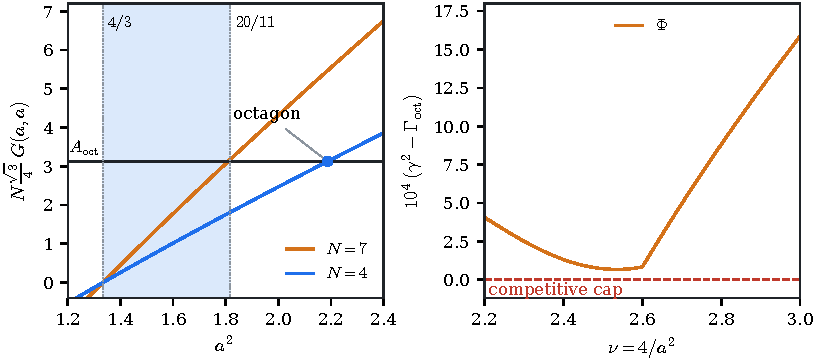
\includegraphics[width=\textwidth]{figures/fig-forward-window.pdf}
\caption{The two sides of the case F contradiction. Left: the cost $N\frac{\sqrt3}4G(a,a)$ of $N$
equal edges against $a^2$, for $N=4$ and $N=7$. Four edges at the octagon's margin cost exactly
$\Aoct$ (dot). Seven edges cost more than $\Aoct$ once $a^2\ge20/11$ (\cref{lem:fwd-threshold}),
and $a^2>4/3$ by \cref{lem:fwd-small}, so the least active margin of a long competitive forward
period lies in the shaded band. Right: on that band, under the bounds of
\cref{lem:fwd-budget,lem:fwd-neighbour,lem:fwd-norms}, the proof uses the scalar curve $\Phi$ of
\cref{app:fwd-casimir}. This curve bounds the Casimir at the two vertices on the norm-sum edge;
the other two vertices are estimated separately in the proof.
The curve is strictly convex up to the shape ceiling $\nu=13/5$
and increases thereafter. Its minimum lies above the competitive cap
$\Gamma_{\rm oct}$ (dashed), defined in \cref{cor:fwd-cap}.
The vertical scale is $10^{4}(\gamma^2-\Gamma_{\rm oct})$.}\label{fig:forward}
\end{figure}

\subsection{Estimates for class F}\label{app:forward-estimates}

This subsection proves the scalar inequalities of \cref{sec:forward}, in its notation: $\nu=4/a^2$,
the ratios $z,w,\hat p,\hat d\ge1$, $\hat s_\pm$, $\hat K$, $\hat K_\pm$, the factors $h,q,k$, the
row coefficients $A,B,\eta,n_1,n_2$ and the floor $F_x(r)$ of \cref{prop:fwd-window}. Throughout,
\[
f(r)=\frac{r-r^{-1}}2-\log r,\qquad \beta(y)=\frac{y^2+y+1}{(1+y)^2}=1-\frac1{1+y}+\frac1{(1+y)^2},
\]
so that $\beta(w)$ is the value $1-x+x^2$ of the floor $F_x$ at $r=1$ for $x=w/(1+w)$.

\subsubsection{The edge function}\label{app:fwd-edge}

Let $G$ be the edge function of \eqref{eq:fwd-cost}. Its partial derivatives are
\begin{align*}
\partial_bG(a,b)&=3a-2b\log(a+b)-\frac{a^2+b^2}{a+b}+b\log(b^2+4)+\frac{b^3}{b^2+4},\\
\partial_a\partial_bG(a,b)&=\frac{2(a^2+ab+b^2)}{(a+b)^2},\qquad
\partial_a\partial_b^2G(a,b)=\frac{2a(b-a)}{(a+b)^3}.
\end{align*}
\begin{enumerate}
\item (Monotonicity) The bound $\log y\ge1-1/y$ at $y=(b^2+4)/(a+b)^2$ gives
  $\partial_bG(a,b)\ge a(a+2b)(b^2-ab+8)/\bigl((a+b)(b^2+4)\bigr)$, which is positive when
  $ab\le8$. So $G$ increases in each argument while the product of its arguments is at most $8$.
  All products of consecutive active margins are below $4$.
\item (Rectangle inequality) Since $\partial_bG(x,\cdot)-\partial_bG(a,\cdot)\ge0$ for $x\ge a$,
  integrating in the second variable gives $G(x,y)\ge G(x,a)+G(a,y)-G(a,a)$ for $x,y\ge a>0$.
\item (Concavity) If $a^2\ge4/3$, then $G(a,\cdot)$ is concave on $[a,4/a]$. Since
  $\partial_a\partial_b^2G\ge0$ for $a\le b$, it suffices to check $\partial_b^2G<0$ at $a=b$ when
  $4/3\le b^2\le4$, and at $a=4/b$. With $\varsigma=4b^2/(b^2+4)\in[1,2]$ one has
  $\partial_b^2G(b,b)=-\log\varsigma-\frac32+\frac54\varsigma-\frac18\varsigma^2$, which increases in
  $\varsigma$ (its derivative is $(\varsigma-1)(4-\varsigma)/(4\varsigma)$) up to the value
  $\frac12-\log2<0$ at $\varsigma=2$; and $\partial_b^2G(4/b,b)=\log\varrho+1-\varrho<0$ with
  $\varrho=b^2/(b^2+4)$.
\item (Scaling) $G(ax,ay)=a^2g_\nu(x,y)$ with
  $g_\nu(x,y)=3xy-\nu-(x^2+y^2)\log(x+y)+\frac12x^2\log(x^2+\nu)+\frac12y^2\log(y^2+\nu)$; we write
  $g_\nu(x)=g_\nu(1,x)$. In particular $g_\nu(1)=3-\nu-\log\frac4{1+\nu}\ge\nu(3-\nu)/(1+\nu)\ge0$
  for $0<\nu\le3$, by $\log y\ge1-1/y$ again; so $G(a,a)\ge0$ when $a^2\ge4/3$.
\end{enumerate}

\subsubsection{Logarithm bounds}\label{app:fwd-logs}

The sum and neighbour comparisons use the following elementary logarithm bounds,
each proved from the sign of a derivative. For $v\ge1$ and $\tau=(v-1)/(v+1)$,
\[
2\tau+\tfrac23\tau^3\le\log v\le2\tau+\frac{2\tau^3}{3(1-\tau^2)},
\]
and for $h\ge1$, $0\le y<1$,
\[
\frac{(h-1)^3}{3h(h+1)}\le f(h)\le\frac{(h-1)^3}{6},\qquad
\log(1-y)\le-y-\frac{y^2}2-\frac{y^3}3 .
\]
The lower bound for $f$ holds because the difference vanishes at $h=1$ and has derivative
$(h-1)^4/(6h^2(h+1)^2)$; this Pad\'e bound is used for the sum and neighbour residuals below and, in the form
$\log v\le\frac{v-v^{-1}}2-\frac{(v-1)^3}{3v(v+1)}$, for other logarithms. The upper bound for
$\log v$ at $v=5/4$ gives $\log\frac54<\frac9{40}$.

\subsubsection{The threshold and the budget}\label{app:fwd-budget}

\runin{The threshold.} With $a_0^2=20/11$ and $\nu_0=11/5$,
$g_{\nu_0}(1)=3-\frac{11}5-\log\frac{20}{16}=\frac45-\log\frac54$, so
$G(a_0,a_0)=\frac{20}{11}\bigl(\frac45-\log\frac54\bigr)>\frac{20}{11}\cdot\frac{23}{40}=\frac{23}{22}$.
The midpoint inequality for $1/t$ on $[1,\sqrt2]$ gives $\log2>12-8\sqrt2$, and hence
\[
 \Aoct<\frac{8\sqrt3(\sqrt2-1)}{2\sqrt2-1}<\frac{29\sqrt3}{16}.
\]
The second comparison is $70\sqrt2<99$, whose square is $9800<9801$.
Since $\frac{7\sqrt3}{4}\frac{23}{22}=161\sqrt3/88>29\sqrt3/16$, the threshold cost exceeds
$\Aoct$, which proves \cref{lem:fwd-threshold}.

\begin{lemma}[Joint concavity of the exterior cost]\label{lem:fwd-joint-concavity}
The function $\mathcal F(\nu,x)=5g_\nu(1)+2g_\nu(x)$ is strictly concave on
$1\le x\le\nu\le3$.
\end{lemma}

\begin{proof}
Put $D=x^2+\nu$ and
\[
 \mathcal E(\nu,x)=-\partial_x^2g_\nu(x)-\frac{\nu^2}{2D^2}.
\]
We first show $\mathcal E>0$. Differentiation gives
\[
 \partial_x^2g_\nu(x)=-\log\frac{(1+x)^2}{D}
  +\frac{2(x+2)}{(x+1)^2}-\frac{\nu(x^2+3\nu)}{D^2},\qquad
 \partial_\nu\mathcal E=\frac{\nu(2x^2-\nu)}{D^3}.
\]
At $\nu=x$, writing $y=1/(x+1)$,
\[
 \mathcal E(x,x)=-\log(1-y)-y-\frac{y^2}{2}
 =\int_0^y\frac{t^2}{1-t}\,\dd t>0.
\]
For larger $\nu$, substitution of $\nu=x^2t$ gives
\[
 \mathcal E(\nu,x)-\mathcal E(x,x)
 =\int_{1/x}^{\nu/x^2}\frac{t(2-t)}{(1+t)^3}\,\dd t.
\]
The lower endpoint is at most one and the upper endpoint at most three. If the upper endpoint
is at most two, the integrand is nonnegative. Otherwise the integral is at least the integral
over $[1,3]$, which is positive: with $k(t)=t/(1+t)^3$, pair the two points $2\pm z$ to get
\[
 \frac{(2-z)z}{(3-z)^3}-\frac{(2+z)z}{(3+z)^3}
 =z\bigl(k(2-z)-k(2+z)\bigr)>0\qquad(0<z\le1),
\]
since $k$ decreases on $[1,3]$. Thus $\partial_x^2g_\nu(x)<-\nu^2/(2D^2)$ everywhere.

The other entries of the Hessian of $\mathcal F$ are
\[
 \mathcal F_{\nu\nu}=-\frac6{(1+\nu)^2}-\frac{x^2}{D^2}<0,\qquad
 \mathcal F_{\nu x}=\frac{2\nu x}{D^2}.
\]
Its determinant is therefore greater than
\[
 \frac{3\nu^2}{D^2}
 \left(\frac2{(1+\nu)^2}-\frac{x^2}{D^2}\right)>0.
\]
For the last sign use $D^2\ge4\nu x^2$ and $(1+\nu)^2<8\nu$ on $1\le\nu\le3$.
The Hessian is negative definite, proving strict concavity.
\end{proof}

\runin{The budget.} The rectangle inequality gives the seven-entry bound in Step~3.
For an increasing concave function $\phi$ on $[1,M]$ and four points with sum at least
$\sigma$, where $1<\sigma-3\le M$,
\[
 \phi(x_1)+\phi(x_2)+\phi(x_3)+\phi(x_4)\ge3\phi(1)+\phi(\sigma-3).
\]
Indeed, first lower the points until their sum is $\sigma$. Each then lies in $[1,\sigma-3]$;
summing the lower chord bound on that interval proves the claim. If
$\hat p+z+w+\hat d\ge(5\nu+1)/3$, apply it to $\phi=g_\nu$ and
$x_*=(5\nu-8)/3$ to obtain
\[
 \Aoct\ge\frac{\sqrt3}{\nu}\bigl(5g_\nu(1)+2g_\nu(x_*)\bigr)
 =\frac{\sqrt3}{\nu}\mathcal F(\nu,x_*).
\]
The line $(\nu,x_*)$ lies in $1\le x\le\nu\le3$. By \cref{lem:fwd-joint-concavity},
$\mathcal F(\nu,x_*)$ lies above the chord joining its values at $\nu=11/5$ and $\nu=3$.
After division by $\nu>0$, that chord is a weighted average of the two endpoint ratios.
It therefore suffices to bound both endpoint ratios below by $29/16$.

At $\nu=11/5$, $x_*=1$ and the threshold estimate gives
\[
 \frac{\mathcal F(11/5,1)}{11/5}>
 \frac{161}{88}>\frac{29}{16}.
\]
At $\nu=3$, $x_*=7/3$, $g_3(1)=0$, and
\[
 g_3(7/3)=4-\log\frac53-\frac{49}{18}\log\frac{25}{19}.
\]
Use $\log v<(v-1)/\sqrt v$ for $v>1$, which is $t<\sinh t$ at $t=\frac12\log v$.
Then
\[
 g_3(7/3)>4-\frac2{\sqrt{15}}-\frac{49}{15\sqrt{19}}
 >4-\frac{17}{32}-\frac34=\frac{87}{32}.
\]
The two rational comparisons follow by squaring: $64^2<15\cdot17^2$ and
$196^2<19\cdot45^2$. Hence $\mathcal F(3,7/3)/3>29/16$ as well.
The exterior cost thus exceeds $29\sqrt3/16>\Aoct$, a contradiction. This proves
\cref{lem:fwd-budget}.

\subsubsection{The centered system}\label{app:fwd-centered}

The following identities hold for $\nu,z,w,h>0$, $h\ne1$; each is an equality of rational
expressions in the variables and the logarithms.
\begin{enumerate}
\item (Floors) $F_{z/\hat s_-}(h)=\frac34+L(z,h)$ with
  \[
  L(z,h)=\frac{(z-1)\bigl(z-1+2z(h-1)\bigr)}{4\hat s_-^2}+\frac{zh}{\hat s_-}\cdot\frac{f(h)}{h-1},
  \]
  and $L(z,h)\ge0$ for $z\ge1$, $h>1$.
\item (Central row) $\frac34(\hat s_-+\hat s_+)-A=e_0-\varphi$.
\item (Left row) With $\zeta=z-1$ and $H=h-1$, the quantity $r=\eta A-B-\frac34(n_1+n_2)$ of
  \eqref{eq:fwd-centered} is given by
  \begin{align*}
  8\hat s_-\hat K_-\,r={}&(3-\nu)\zeta(3-\nu+2\zeta)\\
  &+H\bigl((3-\nu)^2(\zeta^2+4\zeta+2)+8(3-\nu)\zeta z\bigr)
  +2H\zeta^2(8+4\zeta-\zeta^2)\\
  &+\frac{4\hat s_-H^2z(3-\nu+4\zeta+\zeta^2)}{h}\\
  &+8\hat s_-\hat K(1+\hat s_-H)\,\varphi-8\hat s_-\hat K_-\,zf(h).
  \end{align*}
  It depends on $w$ only through $\varphi$.
\item (Coefficients) $\hat s_-\hat K_-(n_2-n_1)=\hat K(\hat s_-\hat s_+-\hat K)
  +H\bigl(\hat s_-^4-\hat K^2+\hat K\hat s_-^2(\hat s_+-\hat s_-)\bigr)$, which is positive for
  $\nu<3$, $1\le z\le w$, $h\ge1$, because $\hat s_-\hat s_+\ge4>\hat K$ and
  $\hat s_-^4\ge16>\hat K^2$.
\end{enumerate}
Two monotonicity facts complete the setup. The floor increases in the factor: for $x\ge1/2$,
$\partial_rF_x(r)=x^2-x\,(r-1-\log r)/(r-1)^2\ge x^2-x/2\ge0$, since
$r-1-\log r\le(r-1)^2/2$. And in the variable $w$, with $\nu,z,h$ fixed,
\[
n_2(w)-n_2(z)=\eta\,(w-z),\qquad A(w)-A(z)\le(w-z)\,\beta(w)\qquad(z\le w),
\]
because $\partial_wA=\beta(w)$ and $\beta'(y)=(y-1)/(1+y)^3\ge0$ for $y\ge1$.

\subsubsection{The three residual signs}\label{app:fwd-signs}

\runin{Lowering the larger neighbour.} The residuals of \cref{sec:forward} depend on $w$ through
$A$, $n_2$, $\varphi$ and the opposite floor. For $\mathcal E_v=r-n_1L(z,h)-n_2/64$ the increments
above give
$\mathcal E_v(w)-\mathcal E_v(z)\le\eta(w-z)\bigl(\beta(w)-\frac{49}{64}\bigr)\le0$, since
$\beta(w)\le\beta(4/3)=37/49<49/64$. For
$\mathcal E_\Sigma=r-n_1/32-(n_2-n_1)L(w,\hat s_+^2/\hat K_+)$ put $V(w)=\frac34+L(w,\hat s_+^2/\hat K_+)$,
the floor at the least admissible factor; then $V(w)\ge\beta(w)$, and $V$ is nondecreasing in $w$
(the coefficients of $L$ increase in $w$, $hf(h)/(h-1)$ increases in $h$, and
$\hat s_+^2/\hat K_+$ increases in $w$), so
\[
\mathcal E_\Sigma(w)-\mathcal E_\Sigma(z)
\le\eta(w-z)\bigl(\beta(w)-V(w)\bigr)-(n_2(z)-n_1)\bigl(V(w)-V(z)\bigr)\le0 .
\]
The neighbour residual is lowered in the same way to $w=\max(z,4/3)$. After lowering, $w=z$ for
$\mathcal E_\Sigma$ and $\mathcal E_v$, and the factor ranges over the symmetric domain
\begin{equation}\label{eq:fwd-symdomain}
1\le z\le\tfrac43,\quad\ 1+\tfrac65z\le\nu<3,\quad\
\frac{(1+z)^2}{z^2+\nu}\le h\le\frac{(1+z)(5\nu-2-3z)}{3(z^2+\nu)};
\end{equation}
the lower bound for $\nu$ is exactly the condition that the interval for $h$ be nonempty.

\runin{Concavity in the factor.} As functions of $h$, with the other variables fixed, the three
residuals have the form $c_0+c_1h+c_2h^2+c_{-1}/h+(d_0+d_1h)\log h$, with second derivative
$(2c_2h^3+2c_{-1}+d_1h^2-d_0h)/h^3$. For $\mathcal E_v$ and $\mathcal E_N$ it equals
$-zP(h)/(\hat K_-h^3)$ with
\[
P(h)=(\nu-z)h^2(2zh-\hat s_-)+\hat K_-h-2z\hat s_- .
\]
For $h\ge1$, $P'(h)=2(\nu-z)h(3zh-\hat s_-)+\hat K_->0$, and at the least factor
$H_0=\hat s_-^2/\hat K_-$,
\begin{gather*}
P(H_0)=-\frac{\hat s_-(2z+1-\nu)}{\hat K_-^3}\,Q(\nu,z),\\
Q(\nu,z)=(1-z)\nu^2-z(z^3+7z^2+5z+3)\nu+z^2(z^4+2z^3+6z^2+5z+2).
\end{gather*}
On the domains of these residuals, $1\le z\le5/3$, $\nu<3\le2z+1$ and $\nu\ge1+6z/5>z+1$.
Since $Q$ decreases in $\nu$, it suffices to evaluate it at $z+1$:
\[
 Q(z+1,z)=z^3\bigl(z^2(z+1)-2z-8\bigr)-7z^2-2z+1<0.
\]
Indeed, $z^2<3$ gives $z^2(z+1)-2z-8<z-5<0$, and $7z^2+2z-1>0$ for $z\ge1$.
So $P\ge0$ on $[H_0,\infty)$, and $\mathcal E_v,\mathcal E_N$ are concave in $h$ there. A concave
function on an interval lies below its tangent at an endpoint, and the tangent is affine, so the
residual is negative on the interval as soon as the tangent is negative at both endpoints. This
leaves two values for each residual: the value at one endpoint and the tangent's value at the
other. The sum residual is treated in the variable $\tau=(h-1)/h$ instead (below).

\begin{lemma}[The individual norm residual]\label{lem:fwd-individual}
On the symmetric domain \eqref{eq:fwd-symdomain}, $\mathcal E_v<0$.
\end{lemma}

\begin{proof}
Put $a=(z-1)/(z+1)$, $b=1-a$, and write the least and greatest admissible factors as
\[
 h_0=\frac{(1+z)^2}{z^2+\nu}=1+t=:\ell,\qquad
 h_+=\frac{(1+z)(5\nu-2-3z)}{3(z^2+\nu)}.
\]
Then $0\le a\le1/7$, $0<t\le1/4$, and
\begin{gather*}
 z=\frac{1+a}{b},\qquad
 \nu=\frac4{b^2\ell}-z^2,\qquad
 \xi:=\frac{\hat K}{\hat K_-}=1-a\ell\ge\frac{23}{28},\\
 h_+-\ell=\frac{2[1-a^2-(4+a^2)t]}{3b}.
\end{gather*}
Thus $t\le t_*(a):=(1-a^2)/(4+a^2)\le1/4$.
Define the value and the other endpoint of its tangent by
\[
 \mathcal V(a,t)=\mathcal E_v(\ell),\qquad
 \mathcal T(a,t)=\mathcal V(a,t)
       +(h_+-\ell)\,\partial_h\mathcal E_v(\ell).
\]
The product $n_1F_{z/\hat s_-}(h)$ has a removable singularity at $h=1$, since $n_1$ contains
$h-1$. After cancellation both endpoint functions extend smoothly to the rectangle
$0\le a\le1/7$, $0\le t\le1/4$.
The original residual is concave in $h$, as proved above. It is therefore enough to show
$\mathcal V<0$ and $\mathcal T<0$ on the actual domain.

\runin{Convexity of the value.} The logarithmic part of $\mathcal V$ is
\[
 c\log\ell+\frac{(b+2t)\xi}{b}\log\xi,\qquad
 c=\frac{a(a^2+3)\ell+2(1-a^2)-(1+3a^2)\ell^2}{b^2}.
\]
The rational part has third $t$-derivative $3(1+a)^3/b^2>0$.
The third derivative of $c\log\ell$ is
\[
 \frac{4(1-a^2)-2(1+3a^2)\ell^2-a(a^2+3)\ell}{b^2\ell^3}>0.
\]
Its numerator decreases in both variables and is positive at $a=1/7$, $\ell=5/4$.
The last logarithmic term has third derivative
$a^2[a(b+2t)+6\xi]/(b\xi^2)\ge0$.
Moreover
\[
 \mathcal V_{tt}(a,0)
 =\frac{a}{16b^2}\left[2+a-33a^2+64b(-\log b-a)\right]\ge0,
\]
since $-\log b\ge a$ and $2-33/49>0$. Hence $\mathcal V$ is convex in $t$.
Its lower edge is negative for $a>0$:
\[
 \mathcal V(a,0)=b\log b+\frac{a(31-16a)}{32}
 \le\frac{a(16a^2-1)}{32}<0,
\]
using $\log(1-a)\le-a-a^2/2$. At $a=0$ this edge value is zero.

We show that the upper edge is convex in $y=z-1\in[0,1/3]$.
Put $S=y+2$, $D=2-ty$, so $\xi=D/S$ and $q=\ell S/D$.
Differentiation of the logarithmic terms, with their common terms combined, gives
\begin{align*}
 \mathcal V_{yy}={}&2t^3+\frac{49}{32}t^2
 -\frac{\ell(16t^2+15t-1)}{8S^3}-\frac{12\ell}{S^4}\\
 &-2t\ell\log\ell-\frac{4\ell}{S^3}\log q
       +\frac{4\ell(3\ell+t^2S)}{DS^3}.
\end{align*}
The inequalities $\log\ell\le t$, $\log q\le q-1$ therefore give
\[
 \mathcal V_{yy}\ge-\frac{15t^2}{32}
 -\frac{\ell(16t^2+15t-1)}{8S^3}-\frac{12\ell}{S^4}
 +\frac{4\ell[5\ell-S(1+2t-t^2)]}{DS^3}.
\]
At $t=1/4$ the right side equals
\[
 \frac5{S^4}\left[
 \frac{3(S-1)}8+\frac{y(19-43y)}{8(8-y)}
             -\frac{15S}{128}-\frac{3S^4}{512}\right]>0.
\]
Indeed, the second term in brackets is nonnegative, while $S^4\le16+52y$ follows by
integrating $4S^3\le4(7/3)^3<52$. The remaining terms are at least $3(1-y)/64>0$.

It remains to check the two ends of this convex upper edge. Set $L_0=\log(5/4)$.
The reciprocal integral gives $1/5<L_0<9/40$, the latter by its trapezoid bound.
At $y=0$,
\[
 \mathcal V(0,1/4)=\frac{56L_0-13}{128}<0.
\]
At $y=1/3$, write $\mathcal V=R+C_L\log\ell+C_M\log\xi$. Direct substitution gives
\begin{gather*}
 R=-\frac{13}{84^2},\qquad
 C_L=\frac83-\frac{15}{14}-\frac{65}{144}\in(0,5/4),\qquad
 C_M=\frac14-\frac1{48}+\frac{15}{14},\\
 15C_M-17C_L=\frac4{63},\qquad \ell\xi=\frac{115}{112},\quad \xi=\frac{23}{28}.
\end{gather*}
Combine the logarithms before bounding them. Their sum is less than
\[
 C_L\left[\frac3{112}
       -\frac2{15}\left(\frac5{28}+\frac{25}{2\cdot28^2}\right)\right]
 =\frac{C_L}{1176}<\frac{5}{4\cdot1176}.
\]
Here we used $\log(115/112)<3/112$ and
$\log(23/28)<-5/28-25/(2\cdot28^2)$.
As $84^2=6\cdot1176$, this proves
$\mathcal V<( -13/6+5/4)/1176<0$ at the second corner.
Convexity in $y$ gives a strictly negative upper edge. Convexity in $t$, together with the
lower edge, now proves $\mathcal V<0$ throughout the rectangle with $t>0$.

\runin{Monotonicity of the other tangent endpoint.}
We prove $\mathcal T_t\ge0$ on the rectangle. Its logarithmic part is
\[
 c\log\ell+\frac{\xi U}{3b^2}\log\xi,\qquad
 U=b(7+a)-kt,\quad k=2(5+3a+2a^2),
\]
where $c=(p_2\ell^2-p_1\ell+p_0)/(3b^3)$ and
\begin{align*}
 p_2&=(1+3a^2)(5+3a+2a^2),\\
 p_1&=10(1+3a^2)+a\bigl[8(4+a^2)-3b(a^2+3)\bigr],\\
 p_0&=6b(1-a^2)+40a.
\end{align*}
All three coefficients are positive; for $p_1$ use $b\le1$.
The rational part has third derivative
\[
 -\frac{(1+a)^3(13+3a+4a^2)}{b^3}
 -\frac{5(1-16a^2)}{8b^2\ell^4}
 <-\frac{13(1+a)^3}{b^3}.
\]
The logarithmic term $c\log\ell$ contributes at most
$(2p_2+p_1+2p_0)/(3b^3)$, since $\ell\ge1$. It is absorbed by this negative term:
\[
 13(1+a)^3-\frac{2p_2+p_1+2p_0}{3}
 =\frac{7+20a+a^2(56+4a-15a^2)}3>0.
\]
The third derivative of the last logarithmic term is
\[
 \frac{a^2(aU-3k\xi)}{3b^2\xi^2}\le0,
\]
since $aU\le7a\le1$, $k\ge10$ and $\xi\ge23/28>3/4$.
Thus $\mathcal T_{ttt}<0$, so $\mathcal T_t$ is concave in $t$.

On its lower edge, substitute $-\log b\ge a+a^2/2$ in the exact derivative to obtain
\[
 96b^2\mathcal T_t(a,0)
 \ge a\left[23+11a-2a^2(81+106a+40a^2)\right]\ge0.
\]
The bracket is positive: $81+106a+40a^2<100$ on $a\le1/7$, so it exceeds
$23-200/49>0$. Consequently this edge is strictly positive for $a>0$, and zero at $a=0$.

On the upper edge let $W(a)=\mathcal T_t(a,1/4)$.
Its coefficient of $\log\xi$ is
$(7a^3+11a^2+2a-10)/(3b^2)<0$, since $7a^3+11a^2+2a\le26/49<1$.
Replacing $\log\xi=\log(1-5a/4)$ by $-5a/4$ therefore gives a lower bound
$W(a)\ge\mathcal G(a)$.
After two derivatives in $b$, its rational terms combine into three reciprocal kernels:
\begin{gather*}
 \mathcal G_{bb}=-\frac{113}{48}
       +C_2(3/b-1/b^2)''+C_3(6/b-1/b^3)''+D_0(-1/b)'',\\
 C_2=\frac{92}{3}L_0-\frac{173}{48},\qquad
 C_3=\frac{133}{48}-\frac{20}{3}L_0,\qquad
 D_0=\frac{28}{3}L_0-\frac{113}{320}.
\end{gather*}
The bounds $1/5<L_0<1/4$ make all three weights positive. The kernels are concave:
\[
 (3/b-1/b^2)''=-\frac{6(1-b)}{b^4},\quad
 (6/b-1/b^3)''=-\frac{12(1-b^2)}{b^5},\quad
 (-1/b)''=-\frac2{b^3}.
\]
Thus $\mathcal G_{bb}<0$ on $6/7\le b\le1$.
At $a=0$, $\mathcal G$ has value $5L_0/6-49/480>0$.
At $a=1/7$, the rational part of $W$ exceeds $-4/5$, its $L_0$ coefficient exceeds $1/5$,
and minus its $\log\xi$ coefficient exceeds $30/7$. Thus
\[
 \mathcal G(1/7)>\frac1{25}+\frac{75}{98}-\frac45=\frac{13}{2450}>0.
\]
Both endpoints are positive, so $W\ge\mathcal G>0$ throughout the upper edge.
Concavity in $t$ now gives $\mathcal T_t\ge0$ on the whole rectangle.

Finally, at $t=t_*(a)$ one has $h_+=\ell$ and hence
$\mathcal T(a,t_*)=\mathcal V(a,t_*)<0$.
Therefore $\mathcal T(a,t)\le\mathcal T(a,t_*)<0$ on the actual domain.
The two negative endpoint values of the affine tangent prove $\mathcal E_v<0$.
\end{proof}

\begin{lemma}[The sum norm residual]\label{lem:fwd-sum}
On the symmetric domain \eqref{eq:fwd-symdomain}, the residual
$\mathcal E_\Sigma=r-n_1/32-(n_2-n_1)L(z,\hat s_-^2/\hat K_-)$ is negative.
\end{lemma}

\begin{proof}
Put $a=(z-1)/(z+1)$ and $t=(1+z)^2/(z^2+\nu)-1$.
Then $0\le a\le1/7$ and $0<t\le1/4$.
The sum residual has the form
\[
 \mathcal E_\Sigma=A_0+A_1H
       +z\left(\frac{DH^2}{2h}-f(h)\right),\qquad
 H=h-1,\qquad D=a+t+at,
\]
where $A_0,A_1$ are independent of $h$.
The reciprocal lower bound for $f(h)$ gives, with $\tau=H/h$,
\[
 \frac{\mathcal E_\Sigma}{H}\le\Psi(\tau):=
 A_0(1/\tau-1)+A_1
       +z\left(\frac{D\tau}{2}-\frac{\tau^2}{3(2-\tau)}\right).
\]
We first prove $A_0\le0$, and then bound a fixed affine tangent to $\Psi$.

\runin{The constant coefficient of the sum residual.}
The sign $A_0\le0$ in the sum residual has a direct derivative proof.
Write $a=(z-1)/(z+1)$, $b=1-a$, $h_0=1+t$ and $\beta=1-ah_0$.
The coefficient $A_0$ is the value $\mathcal E_\Sigma(1)$ of the continuously
extended row expression. Since $n_1(1)=0$, it does not depend on the
chosen norm threshold. Substitution gives
\[
 A_0=\beta\log\beta+
 \frac{a\beta(ah_0+3t+1)}{bt}\log h_0
 +\frac{a(a+t+at)}{2b}\bigl((1+a)^2h_0-4\bigr).
\]
The quotient $\log h_0/t$ takes its continuous value $1$ at $t=0$.
At fixed $t$, three derivatives in $a$ give
\[
 \partial_a^3A_0=\frac{h_0^3}{\beta^2}-3h_0^2
                 +\frac{12(1+2t)(t-\log h_0)}{b^4}<0.
\]
Indeed $0\le t-\log(1+t)\le t^2/2$, and on
$0\le a\le1/7$, $0\le t\le1/4$,
\[
 \frac{h_0}{\beta^2}\le\frac{5/4}{(23/28)^2}<2,
 \qquad
 \frac{6(1+2t)t^2}{b^4h_0^2}
 \le\frac{9}{25(6/7)^4}<1.
\]
To determine the initial slope and curvature, set $L=\log h_0$.
For $t>0$ the exact values are
\begin{align*}
 \partial_aA_0(0,t)&=\frac{t^3-5t^2+(6t+2)L-2t}{2t},\\
 \partial_a^2A_0(0,t)&=\frac{5t^3-t^2-2t+(2-6t^2)L}{t}.
\end{align*}
The convexity of the reciprocal kernel gives
$L\le t-t^2/(2h_0)$. Both coefficients of $L$ above are positive, so
\[
 \partial_aA_0(0,t)\le\frac{t^2(t-1)}{2h_0}<0,
 \qquad
 \partial_a^2A_0(0,t)\le\frac{2t(t^2-t-1)}{h_0}<0.
\]
At $t=0$ these derivatives have value zero by continuity.
Thus $\partial_a^2A_0$ decreases from a nonpositive initial value,
and $\partial_aA_0$ does likewise. Since $A_0(0,t)=0$, we obtain
$A_0\le0$, with strict inequality when $a>0$.

\runin{A fixed tangent for the sum residual.}
Write
\begin{gather*}
 a=\frac{z-1}{z+1},\qquad b=1-a,\qquad k=\frac{t}{1+t},\\
 r=1-k,\qquad c=a+k,\qquad \bar c=1-c.
\end{gather*}
Thus $0\le a\le1/7$, $0\le k\le1/5$, $z=(1+a)/b$ and
$\beta=\bar c/r$. The actual shape domain is contained in this rectangle.
The tangent to $\Psi$ at $\tau=1/5$ is
\[
 W(a,k,\tau)=A_1+(9-25\tau)A_0
       +z\left[\left(\frac{c}{2r}-\frac{19}{243}\right)\tau
                        +\frac{2}{243}\right].
\]
Since $A_0\le0$, one has
\[
 \Psi''(\tau)=\frac{2A_0}{\tau^3}-\frac{8z}{3(2-\tau)^3}<0.
\]
Concavity therefore gives $\Psi(\tau)\le W(a,k,\tau)$.
The following rational terms come from the left row:
\begin{gather*}
 A_R=1+2z-b+\frac{b^2}{4\bar c},\qquad
 B_1=\frac{2r-(1+a)+(1+a)^2/(2r)}b,\\
 N_1=\frac{2(b-2k)}{b^2r},\qquad
 N_d=\frac{2c(2-c)}{br},\qquad F_R=1+\frac{(1+a)^2}{4r},\\
 R_0=\frac{ac((1+a)^2+4k-4)}{2br^2},\\
 R_1=\frac{2\beta}{b}A_R-B_1-\frac{49}{32}N_1-N_dF_R.
\end{gather*}
Here $49/32=3/2+1/32$ includes the norm threshold.
Pair the two logarithms using
\[
 \ell(k)=\int_0^1\frac{\dd v}{1-kv},\qquad
 J(a,k)=\int_0^1\frac{v\,\dd v}{(1-kv)(1-(a+k)v)}.
\]
Their elementary reciprocal bounds are
\[
 \ell(k)\le\ell_+:=1+\frac k2+\frac{k^2}{3r},\qquad
 J(a,k)\ge J_0:=\frac12+\frac{a+2k}{3}.
\]
The first follows by bounding the geometric remainder under the integral;
the second follows by retaining its constant and linear terms.
For $m=9-25\tau$, the exact logarithmic part of $W$ is
\[
 \frac c{br}\left\{
 [bc+2a(1+m\bar c)]\ell(k)-a\bar c(mb+2)J(a,k)\right\}.
\]
On $0\le\tau\le2/5$, one has $m\ge-1$,
$1+m\bar c\ge c\ge0$ and $mb+2\ge1+a>0$.
The signs therefore give the rational upper bound
\begin{align*}
 U(a,k,\tau)
 ={}&R_1+mR_0
      +z\left[\left(\frac c{2r}-\frac{19}{243}\right)\tau
                        +\frac2{243}\right]\\
 &+\frac c{br}\left\{
 [bc+2a(1+m\bar c)]\ell_+-a\bar c(mb+2)J_0\right\}
 \ \ge W(a,k,\tau).
\end{align*}
All denominators in this expression are positive on the enlarged rectangle.


\runin{The interval for the factor.}
In these coordinates the actual shape domain satisfies
\[
 ab<k\le\frac{1-a^2}{5},\qquad
 k\le\tau\le\tau_c:=\frac{2-2a^2-(7+3a)k}{5-3a-2a^2-10k}.
\]
The denominator $D_c=5-3a-2a^2-10k$ is
$3b+2(1-a^2-5k)>0$. The inequality $\tau_c\le2/5$ is equivalent to
$2ab\le5(1+a)k$, which follows from $k>ab$.
There is also a useful linear ceiling
\[
 \tau_c\le T(k):=\frac8{15}-\frac53k.
\]
Indeed, writing $N_c=2-2a^2-(7+3a)k$ and $d=1-5k\ge0$ gives
\begin{align*}
 T(k)D_c-N_c
 &=\frac2{15}\left(5d^2-a(12+5a)d+12a^2\right)\\
 &\ge\frac2{15}\left(5\left(d-\frac{13}{10}a\right)^2
                                      +\frac{71}{20}a^2\right)\ge0.
\end{align*}
Thus it suffices to prove negativity of the affine function $U$ at
$\tau=k$ and at $\tau=\min(2/5,T(k))$.
The two upper ceilings meet at $k=2/25$.


\runin{The lower sum endpoint.}
Set $X(a,k)=U(a,k,k)$. We prove $X<0$ on the whole rectangle.
First define
\begin{align*}
 \mathcal F(a)&=\frac{1+a}{6b}
        \left[(1+30a)(1+a)^2+15ab^2\right],\\
 Q(a)&=\frac{43}{48}
   +a\left[\frac{39}{2}-\frac{177}{16b}
                         -\frac{15(1+b)}{8b^2}\right]
   +a^2\left[\frac{37}{3}+\frac a3-\frac{16a^2}{3}\right].
\end{align*}
Differentiating the displayed row expression gives
\[
 X_{kkk}=\frac{50a(1-2a)}b
       +\frac{6Q(a)}{r^4}+\frac{6(1-5k)\mathcal F(a)}{r^5}>0.
\]
Indeed $\mathcal F>0$, and $b\ge6/7$ gives
\[
 \frac{177}{16b}\le\frac{413}{32}<13,\qquad
 \frac{15(1+b)}{8b^2}\le\frac{455}{96}<\frac{19}{4}.
\]
The first bracket in $Q$ is consequently greater than $7/4$;
the second is greater than $12$, so $Q\ge43/48>0$.
The remaining factors are nonnegative since $a\le1/7$ and $k\le1/5$.

To determine the initial curvature, let $I(a)=X_{kk}(a,0)$. A second
differentiation in $a$ gives
\[
 I''(a)=\frac43\left[41-12a(11+8a)\right]
          +\frac{8(35b-9)}{3b^4}+\frac{6-b}{4b^4}>0.
\]
Each summand is positive: $a<1/6$ gives
$12a(11+8a)<74/3<41$, and $6/7\le b\le1$ handles the others.
Since $I(0)=17/8>2$ and $I'(0)=-199/24>-9$, its tangent gives
\[
 X_{kk}(a,0)=I(a)\ge I(0)+aI'(0)>2-9a\ge\frac57>0.
\]
Together with $X_{kkk}>0$, this proves that $X$ is strictly convex in $k$.

It remains to check its two $k$ edges. At $k=0$ the row simplifies to
\[
 bX(a,0)=-\frac1{16}+\frac{2(1+a)}{243}+\frac{a^2}{2}
       -\frac{a^3}{6}\left[(2-a)(11-18a)+4a\right].
\]
The final bracket is positive. Moreover
$2(1+a)/243<1/72$ and $a^2/2<1/72$, whence
$bX(a,0)<-1/16+1/36<0$.

For the upper edge put $Y(a)=X(a,1/5)$ and
\[
 H(b)=20b^2-\frac{393}{16}b-\frac23
                       +\frac{119}{16b^3}-\frac{45}{16b^4}.
\]
The exact identities
\[
 H(b)-Y''(a)=\frac{101}{4320b^3}>0,\qquad
 H''(b)=40+\frac{357b-225}{4b^6}>0
\]
reduce its curvature to two scalar values:
$H(6/7)<-2/5$ and $H(1)<-2/5$.
Convexity of $H$ therefore gives $Y''<-2/5$ throughout the interval.
At the midpoint $m=1/14$, direct substitution in the displayed row gives
\[
 Y(m)+\frac54Y'(m)^2<-\frac1{900}.
\]
The quadratic tangent bound now yields
\[
 Y(a)\le Y(m)+Y'(m)(a-m)-\frac{(a-m)^2}{5}
       \le Y(m)+\frac54Y'(m)^2<-\frac1{900}.
\]
Both $k$ edges are negative. Convexity in $k$ gives $X(a,k)<0$ everywhere
on the rectangle, proving negativity of the lower sum endpoint.


\runin{The upper endpoint of the sum residual.}
Put $k_c=2/25$ and define
\begin{equation}\label{eq:fwd-sigma-upper-two-functions}
 \begin{aligned}
 H(a,k)&=U(a,k,2/5)<0&&\quad(0\leq k\leq k_c),\\
 G(a,k)&=U(a,k,T(k))<0&&\quad(k_c\leq k\leq1/5).
 \end{aligned}
\end{equation}
All the estimates below hold on the independent rectangle
$0\leq a\leq1/7$, $0\leq k\leq1/5$ wherever the indicated functions
are used; no enlargement of the physical cost interval is needed.

The useful derivative structure of $U$ comes from its original row.
Put
\[
 m=9-25\tau,\qquad \ell_+=1+\frac k2+\frac{k^2}{3r},\qquad
 \mu=\frac{19}{243},\qquad \eta_0=\frac2{243}.
\]
Its simple-pole weight in $b$ is the following displayed row expression:
\begin{align}\label{eq:fwd-sigma-upper-natural-pole}
 \mathcal A(k,\tau)
 &=\frac{2k-1-1/16}{r}
   +\frac{2mk(1+k)}{r^2}+\frac{\tau(1+k)}r+2(\eta_0-\mu\tau)\notag\\
 &\quad+\frac{2(1+k)(1-mk)}r\ell_+
       +\frac{2k(1+k)}r\left(\frac56+\frac{2k}3\right).
\end{align}
The double-pole weight is $-15k/(8r)$. For example, the rational row
contributes $(2k-1-1/16)/(rb)-15k/(8rb^2)$; the remaining terms in
\eqref{eq:fwd-sigma-upper-natural-pole} are, respectively, the $mR_0$
term, the transport term, and the two paired logarithmic moments.
Thus these are the poles of the actual residual majorant.

The nonconstant polynomial quotient in $a$ also has a short form:
\begin{equation}\label{eq:fwd-sigma-upper-natural-quotient}
 U=q_0+q_1a+q_2a^2+q_3a^3+q_4a^4
       +\frac{\mathcal A(k,\tau)}b-\frac{15k}{8rb^2},
\end{equation}
where $q_0=U(0,k,\tau)-\mathcal A(k,\tau)+15k/(8r)$ is independent of $a$ and
\begin{align*}
 q_4&=\frac m{3r},\qquad q_i=-\frac{T_i}{6r^2}\quad(i=1,2,3),\\
 T_3&=m(8k^2-7k+2)+7-4k,\\
 T_2&=2mk(5k^2-4k+3)+3+19k-15k^2,\\
 T_1&=mk^2(4k^2-k+10)+6+10k+11k^2-18k^3+3r\tau.
\end{align*}
To obtain these identities, divide the row only in $b$ and use
$r\ell_+=1-k/2-k^2/6$; the logarithmic approximations are not expanded
into a shape-box polynomial.

\runin{Concavity of the high-$k$ function.}
Write $\mathcal A_G(k)=\mathcal A(k,T(k))$. On $4/5\leq r\leq23/25$ define the
intrinsic pole and central-derivative functions
\begin{align*}
 P(r)&=r^4\mathcal A_G''(1-r),\\
 D(r)&=r^4G_{akk}(0,1-r),\\
 C(r)&=2P(r)-\frac{45}2r-r^4G_{aakk}(0,1-r).
\end{align*}
Differentiating the displayed row and quotient gives
\begin{align*}
 P''&=\frac{200}3r^2(44-25r)>0,\\
 D''&=r^2\left(\frac{5000}3r-164\right)>0,\\
 C''&=\frac{10000}3r^2>2000.
\end{align*}
The endpoint substitutions in the same row give
\[
 \max\{P(4/5),P(23/25)\}<75,\qquad
 \max\{D(4/5),D(23/25)\}<-7.
\]
Convexity extends both bounds across the interval. At $v=6/7$, the row gives
\[
 C(v)-\frac{C'(v)^2}{4000}>149.
\]
The quadratic lower bound from $C''>2000$ therefore proves $C>149$.

The resulting exact mixed-derivative identity is
\begin{align*}
 r^4G_{akk}
 &=D+\frac{896}9ra^3+(112-457k)a^2-Ca\\
 &\qquad+P(b^{-2}-1)-\frac{15}2r(b^{-3}-1).
\end{align*}
On $0\leq a\leq1/7$,
\[
 b^{-2}-1\leq\frac83a,\qquad b^{-3}-1\geq3a.
\]
For the first inequality, multiplication by $b^2$ leaves the positive
factor $a(2-13a+8a^2)/3$; the second follows by multiplying by $b^3$.
Using $a^3\leq a/49$, $a^2\leq a/7$, $112-457k<76$ and
$15r/2\geq6$, we obtain
\[
 r^4G_{akk}<-7+
 \left(\frac{100}{49}+\frac{76}7-149+200-18\right)a
 \leq-7+46a\leq-\frac37<0.
\]
At the central shape, direct cancellation in the row gives
\[
 G_{kk}(0,k)=
 -\frac{40k^4+80k^2(3-2k)+(1-k)}{120(1-k)^4}<0.
\]
Hence $G_{kk}(a,k)\leq G_{kk}(0,k)<0$: $G$ is concave in $k$.

\runin{The tangent at $k=1/6$.}
Let $k_f=1/6$, $F(a)=G(a,k_f)$, and
\[
 B_\ell(a)=F(a)-\frac{13}{150}G_k(a,k_f).
\]
The factor $13/150=k_f-k_c$. Along $\tau=T(k)$, the
values at $k_f$ are
\[
 r_f=\frac56,\qquad \tau_f=\frac{23}{90},\qquad
 m_f=\frac{47}{18},\qquad m'=\frac{125}3,\qquad \tau'=-\frac53.
\]
The explicit weights in
\eqref{eq:fwd-sigma-upper-natural-pole}--\eqref{eq:fwd-sigma-upper-natural-quotient}
give the small scalar bounds
\begin{align*}
 \mathcal A_G(k_f)&>\frac{37}{12},\\
 q_4(k_f)&>0,\qquad 3q_3(k_f)>-7,\qquad
 2q_2(k_f)>-4,\qquad q_1(k_f)>-\frac94,\\
 \mathcal A_G'(k_f)&<\frac{33}2,\\
 4q_4'(k_f)&<72,\qquad3q_3'(k_f)<-36,\qquad
 2q_2'(k_f)<-37,\qquad q_1'(k_f)<-\frac{23}2.
\end{align*}
For clarity, the $q_i$ comparisons require only the displayed products:
for $i=1,2,3$,
\[
 q_i'= -\frac{rT_i'+2T_i}{6r^3},\qquad
 q_4'=\frac{m'r+m}{3r^2},
\]
evaluated at the displayed values above. All $q_i$ and their primes
in these comparisons are restricted to $\tau=T(k)$.

The double pole of $F$ is $-3/(8b^2)$. It follows that
\begin{align*}
 b^3F'
 &>-7a^2b^3-4ab^3-\frac94b^3+\frac{37}{12}b-\frac34\\
 &=\frac1{12}-\frac a3-\frac74a^2
      +a^3\left(\frac{45}4-17a+7a^2\right)>0.
\end{align*}
The first three terms decrease to zero at $a=1/7$, and the cubic
factor is positive. Similarly, the $k$ derivative of the double-pole
weight at $k_f$ gives the negative pole $-27/(5b^3)$ in $G_{ak}$.
The same coefficient bounds yield
\begin{align*}
 G_{ak}(a,k_f)
 &<72a^3-36a^2-37a-\frac{23}2
                +\frac{33}{2b^2}-\frac{27}{5b^3}\\
 &\leq-\frac25-\frac{46}5a+a^2(72a-36)<0.
\end{align*}
Consequently $B_\ell'=F'-(13/150)G_{ak}>0$ as well.
At their common upper shape endpoint, substitution in the original row
gives the two fixed scalar comparisons
\begin{equation}\label{eq:fwd-sigma-upper-fixed-tangent}
 G(1/7,1/6)<-\frac1{900},\qquad
 G(1/7,1/6)-\frac{13}{150}G_k(1/7,1/6)<0.
\end{equation}
Monotonicity therefore proves $F<-1/900$ and $B_\ell<0$ throughout
the shape interval. The $k_f$ tangent to the concave function $G$ is
negative at both ends of $[k_c,k_f]$, proving $G<0$ there.

\runin{A coarse curvature budget on the short right interval.}
Put $a_*=1/7$. The original row has only simple and double poles at
$r=0$, and its polynomial quotient in $k$ has degree three, with
leading coefficient $125a(2a-1)/(9b)$. Define its actual Laurent weights
\[
 f=\left[r^2G(a_*,1-r)\right]_{r=0},\qquad
 e=\left[\frac{d}{dr}\{r^2G(a_*,1-r)\}\right]_{r=0},
\]
where the bracketed rational functions have removable singularities.
Set $\alpha_L=-2e$, $\beta_L=6f$ and
$\kappa_L=G_{kk}(a_*,0)+\alpha_L-\beta_L$. Elementary partial fractions give
\[
 Z(k):=G_{kk}(a_*,k)=-\frac{625}{63}k+\kappa_L
                         -\frac{\alpha_L}{r^3}+\frac{\beta_L}{r^4}.
\]
The needed bounds are deliberately coarse:
\begin{equation}\label{eq:fwd-sigma-upper-laurent-budget}
 \kappa_L>\frac{21}2,\qquad \alpha_L<35,\qquad \beta_L>\frac{45}2.
\end{equation}
Here is an explicit original-row evaluation for these comparisons.
Set $p=1+a$, $M=112/3$, $N=125/3$ and
\[
 A_p=1+2a-(1+2M)a^2,\qquad B_p=-b+2a(M+Na).
\]
Its double-pole weight is
\[
 f(a)=\frac{p^3}2\left(\frac{Ma}b-1\right)+\frac{pA_p}{3b},
 \qquad f(1/7)>\frac{15}4.
\]
For the simple pole, the rational row and transport terms give
\[
 e_{\rm rat}(a)=\frac p{b^2}
       \left(\frac{119}{240}-3a+\frac{17}{30}a^2+a^3\right)>0,
\]
since $119/240>3/7$. The remaining original-row residues are
\begin{align*}
 e_m(a)&=-\frac{ap\{Np^2+M(a+5)\}}{2b},\\
 e_\ell(a)&=\frac{(5p-2)A_p+2pB_p}{6b},\\
 e_J(a)&=\frac{a^2p(Mb+2)(7+2a)}{6b}.
\end{align*}
At $a_*$ these satisfy $e_m>-47/2$, $e_\ell>44/9$ and $e_J>10/9$.
Their sum with $e_{\rm rat}>0$ gives $e>-47/2+6=-35/2$.
Finally the constant polynomial term in $Z$ gives
\[
 \kappa_L=\frac{2\{1250/343-427/49+90-3\}}{108/7}
          >\frac{2\cdot569}{108}>\frac{21}2,
\]
using $1250/343>3$ and $427/49=61/7$. This proves
\eqref{eq:fwd-sigma-upper-laurent-budget} from the row itself.

For $1/6\leq k\leq1/5$ we have $4/5\leq r\leq5/6$.
The function $(45/2-35r)/r^4$ decreases there, since its derivative is
$(105r-90)/r^5<0$. Hence
\[
 Z(k)>-2+\frac{21}2-\frac{20}3\left(\frac65\right)^4>-6.
\]
Since $G_{akk}<0$, also $G_{kk}(a,k)\geq Z(k)>-6$.
We already know $G(a,1/6)<-1/900$, while the lower-endpoint proof gives
$G(a,1/5)=Y(a)<-1/900$. Convexity of $G+3k^2$ now gives
\[
 G(a,k)<-\frac1{900}+3(k-1/6)(1/5-k)
       \leq-\frac1{900}+\frac1{1200}=-\frac1{3600}<0.
\]
This proves the whole high-$k$ assertion in
\eqref{eq:fwd-sigma-upper-two-functions}.

\runin{The low-$k$ function.}
In $H=U(a,k,2/5)$ the fixed-tangent multiplier is $m=-1$.
Differentiating its original row in $k$ gives
\[
 H_k=2A_2k+A_1+\frac E{r^2}-\frac{2F_p}{r^3},\qquad
 H_{kk}=2A_2+\frac{2E}{r^3}-\frac{6F_p}{r^4},
\]
where
\[
 A_2=-\frac{4a^2+5a+1}{6b},\quad
 A_1=-\frac{10a^3+15a^2+10a+5}{6b},\quad
 F_p=\frac{(1+a)^3}{6b},
\]
and the simple-pole weight is exposed by the positive difference
\[
 E-\frac{15}2F_p
 =\frac{1+a}{240b^2}
   \{43-220a+12a^2+20a^3(15-14a-4a^2)\}>0.
\]
Indeed $43-220a\geq81/7>0$, and the last bracket is positive.
For $k\leq k_c$, $r\geq23/25$. Therefore
\[
 H_{kk}>2A_2+\frac{(15r-6)F_p}{r^4}
       \geq-\frac{44}{63}+\frac{39}5\frac16
       =\frac{379}{630}>0.
\]
At $k=0$,
\[
 H_k>A_1+\frac{11}2F_p
       =\frac{1+13a+3a^2-9a^3}{12b}>0.
\]
Thus $H$ increases in $k$, and $T(k_c)=2/5$ gives
$H(a,k)\leq H(a,k_c)=G(a,k_c)<0$.
Both assertions in \eqref{eq:fwd-sigma-upper-two-functions} follow.
Together with the negative lower $\tau$ endpoint and affine dependence
on $\tau$, this proves $U<0$ on the actual forward window and hence
$\mathcal E_\Sigma<0$ for the norm-sum threshold $1/32$.

\end{proof}


\runin{The neighbour residual.}
The residual in Step~4 is
\[
 \mathcal E_N=\eta A-B-n_1F_{z/\hat s_-}(h)
             -n_2F_{w/\hat s_+}(\hat s_+^2/\hat K_+).
\]
For $w\ge4/3$, lowering $w$ to $\max(z,4/3)$ leaves two faces.
On the symmetric face $w=z\in[4/3,5/3]$, the factor budget gives
$\nu\ge1+6z/5$. We first prove that the value at the least factor is negative.

\begin{lemma}[The symmetric neighbour value]\label{lem:fwd-neighbour-value}
Let $4/3\le z\le5/3$, $1+6z/5\le\nu<3$ and $w=z$.
The value of $\mathcal E_N$ at $h_0=(1+z)^2/(z^2+\nu)$ is strictly negative.
\end{lemma}

\begin{proof}
Put $a=(z-1)/(z+1)$, $b=1-a$, $p=1+a$ and $h_0=1+t=:\ell$.
The physical domain is contained in
\[
 \frac17\leq a\leq\frac14,\qquad \frac18\leq t\leq\frac14.
\]
Indeed, $\nu<3$ gives
$t>2(z-1)/(z^2+3)\geq6/43>1/8$; the rational function increases
on $4/3\leq z\leq5/3$. For the upper bound, $\nu\ge1+6z/5$ and
$5(z^2+1+6z/5)-4(z+1)^2=(z-1)^2\ge0$ give $h_0\le5/4$.
We prove the sign on this whole rectangle.

Writing $\beta=1-a\ell$, the original row at $h_0$ has the exact form
\[
 V(a,t):=\mathcal E_N(h_0)=R+C_L\log\ell+C_M\log\beta,
\]
where
\begin{align*}
 R={}&\frac{p^3(1+2a-a^2)}{2b^2}\ell^3
      -\frac{ap(13+4a-a^2)}{2b^2}\ell^2\\
    &-\frac{a^4-4a^3-14a^2-8a+9}{2b^2}\ell+\frac{4p}b,\\
 C_L={}&-\frac{A}{b^2}\ell^2+\frac{B}{b^2}\ell
                   +\frac{(2-a)p^2}b+\frac{ap}t,\\
 C_M={}&\frac{(b+2t)\beta}b,\qquad
 A=1+2a+6a^2-a^4,\quad B=a^4-a^2+6a+2.
\end{align*}
Both logarithmic weights are positive. For $C_L$, use
\[
 B-\frac54A
 =\frac94a^4-\frac{17}2a^2+\frac72a+\frac34>\frac7{32}>0;
\]
the other terms are positive, and $\ell\leq5/4$.

Use the two integral upper bounds
\begin{align*}
 S(t)&=\frac t6\left(1+\frac8{2+t}+\frac1{1+t}\right)\geq\log(1+t),\\
 P(y)&=-y-\frac{y^2}2-\frac{y^3}3\geq\log(1-y).
\end{align*}
For the first, $(S-\log(1+t))'=t^4/[6(1+t)^2(2+t)^2]\geq0$;
the second integrates the positive geometric-series remainder.
Thus the rational majorant
\[
 \mathcal B(a,t)=R+C_LS(t)+C_MP(a\ell)
\]
satisfies $V\leq\mathcal B$. Its apparent singularity at $t=0$ is
removable, and we use that extension below.

\runin{Decrease in the shape.}
Introduce the positive moment weights
\begin{align*}
 Q&=\ell^3(2t^2+2t+1),\\
 N_1&=t^2(4\ell^4+10\ell^3+19\ell^2+12\ell+1),\\
 N_2&=t\ell(4\ell^4+6\ell^3+10\ell^2+\ell-3),\\
 R_2&=\frac{4t^3(5t+6)}{3(t+2)},\\
 R_1&=\frac{t^2\{16+24t+11t^2+t^3(18+15t+2t^2)\}}
                  {3\ell(t+2)}.
\end{align*}
Differentiating the displayed row gives
\[
 \mathcal B_a=\frac43\ell^4a^3-Qa^2
  -\frac{N_2a}{3(t+2)}-\frac{N_1}{6(t+2)}
  +\frac{2R_2}{b^3}+\frac{R_1}{b^2}.
\]
Since $a\leq1/4$, combine its first two terms. Also
$1/[a(1-a)^n]$ decreases for $a\leq1/(n+1)$. Its maximum for
$n=2,3$ is therefore at $a=1/7$. In particular
$2/(ab^3)<23$ and $1/(ab^2)<10$, so division by $a$ gives
\begin{align*}
 \frac{\mathcal B_a}a
 &\leq-\frac{Q-\ell^4/3}7-\frac{N_2}{3(t+2)}
       -\frac{2N_1}{3(t+2)}
       +23R_2+10R_1.
\end{align*}
The binomial lower bounds for $\ell^j=(1+t)^j$ imply
\begin{align*}
 Q-\ell^4/3&\geq\frac23+\frac{11}3t+9t^2,\\
 N_1&\geq46t^2+96t^3+73t^4,\\
 N_2&\geq18t+73t^2+107t^3+74t^4.
\end{align*}
Furthermore $R_2\leq13t^3/3$, since $7t\leq2$.
For $R_1\leq11t^2/4$, multiply by $3\ell(t+2)/t^2$.
The resulting difference is at least
\[
 \frac12+\frac34t-\frac{33}4t^2>0,
\]
using $18+15t+2t^2\leq22$. This concave quadratic has positive
endpoint values $1/2$ and $11/64$.
Now $1/[3(t+2)]\geq4/27$, and the scalar comparisons
\begin{align*}
 10\frac{11}4-\frac4{27}(73+92)-\frac97&<2,\\
 23\frac{13}3-\frac4{27}(107+192)&<56,\qquad
 -\frac4{27}(74+146)<-32
\end{align*}
give
\[
 \frac{\mathcal B_a}a
 \leq-\frac2{21}-\frac{67}{21}t+2t^2+56t^3-32t^4
 \leq-\frac2{21}-\frac{67}{21}t+14t^2<0.
\]
The last comparison uses
$14-(2+56t-32t^2)=4(1-4t)(3-2t)\geq0$.
The last quadratic is convex on $[0,1/4]$, with negative endpoint
values $-2/21$ and $-1/56$. Hence $\mathcal B$ decreases in $a$.

\runin{Convexity on the remaining edge.}
Let $u(t)=\mathcal B(1/7,t)$. The polynomial part of $\mathcal B$
as a rational function of $t$ has degree five. The coefficients of
$t^5,t^4,t^3$ are respectively
\begin{align*}
 p_5&=\frac{2a^4}{3b}>0,\qquad
 p_4=\frac{a^3(-a^2+9a+1)}{3b}>0.
\end{align*}
The cubic coefficient is determined by the positive-product identity
\[
 6b^2\left(p_3-\frac56\right)
 =a^4(22-42a+8a^2)+13a^3+(19a^2+23a-3)>0;
\]
the last bracket is at least $33/49$. Thus $p_3>5/6$.
The two poles arise from Simpson's reciprocal kernel. Their weights
at $t=-2$ and $t=-1$ are
\[
 C_2=\frac{4p(-a^3+2a^2+13a+2)}{3b^2},\qquad -\frac p{3b}.
\]
At $a=1/7$, $6C_2<49$, because
$2/49+13/7+2<63/16$ and $8p/b^2=112/9$.
All polynomial terms of degree at most two disappear after three
derivatives. We consequently obtain
\[
 u'''>5-\frac{49}{(t+2)^4}+\frac8{3(1+t)^4}>\frac{31}{16}>0.
\]
The initial curvature, computed in the same displayed row, is
\[
 u''(0)=-\frac49+\frac5{3\cdot7^4}>-\frac49.
\]
Integrating on $[0,1/8]$ gives
\[
 u''(1/8)>-\frac49+\frac18
       \left(\frac{31}{16}+\frac83\left(\frac89\right)^4\right)>0.
\]
Thus $u$ is convex on $[1/8,1/4]$. The two fixed scalar substitutions
in the displayed rational definition of $\mathcal B$ give
\[
 \mathcal B(1/7,1/8)<0,\qquad\mathcal B(1/7,1/4)<0.
\]
It follows that $V(a,t)\leq\mathcal B(a,t)\leq u(t)<0$ on the full
rectangle, as required.
\end{proof}

\begin{lemma}[The symmetric neighbour residual]\label{lem:fwd-neighbour-symmetric}
Suppose $w=z$, $4/3\leq z\leq5/3$ and $1+6z/5\leq\nu<3$.
Then $\mathcal E_N(h)<0$ for every $h\geq h_0=(1+z)^2/(z^2+\nu)$.
\end{lemma}

\begin{proof}
Use $a,b,p,t,\ell,\beta$ from \cref{lem:fwd-neighbour-value}.
The actual domain has $1/7\leq a\leq1/4$ and $t>1/8$.
The symmetric exterior budget also gives
\[
 t\leq\frac{1-a^2}{4+a^2}\leq\frac{48}{197},
\]
since this rational function decreases in $a$.
We first prove that the partial derivative of $\mathcal E_N$ in $h$,
holding $z,\nu$ fixed, is negative at $h_0$. Differentiate the original
row before substituting $h=h_0$ and changing to $(a,t)$.
The resulting partial slope is
\[
 D(a,t)=R_D+C_D\log\ell+\frac{2\beta}b\log\beta,
\]
where
\begin{align*}
 R_D={}&\frac{p(-a^4+5a^2+6a+2)}{2b^2}\ell^2
       -\frac{-a^4+9a^2+10a+2}{b^2}\ell\\
      &-\frac{a^3-5a^2-13a+1}{2b^2}+\frac p{2\ell},\\
 C_D={}&-\frac A{b^2}t+\frac{P_D}{b^2}+\frac{K_D}t,\\
 P_D={}&2a^4-2a^3-9a^2+4a+1,\qquad
 K_D=\frac{p(1+2a-a^2)}b.
\end{align*}
The $A$ here is the positive weight from the value proof.
Both logarithmic weights are positive: $K_D>0$, and
\[
 P_D-\frac A4
 =\frac94a^4-2a^3-\frac{21}2a^2+\frac72a+\frac34>\frac1{16}.
\]
Using the same Simpson and geometric upper bounds $S,P$ as before,
define
\[
 \mathcal D(a,t)=R_D+C_DS(t)+\frac{2\beta}bP(a\ell).
\]
Use the continuous extension at $t=0$ for the derivative comparisons below.
Then $D\leq\mathcal D$. We shall prove that this rational majorant is
negative on the physical domain.

\runin{A derivative maximum principle in the shape.}
The derivative in $a$ has the exact reciprocal-kernel form
\[
 \mathcal D_a=-3P_3a^2-2P_2a-P_1+\frac{2R_2}{b^3}+\frac{R_1}{b^2},
\]
with the following positive row weights:
\begin{align*}
 P_3&=\frac{\ell^2(4\ell^2+3)}6,\\
 P_2&=\frac{\ell(4\ell^4+6\ell^3+10\ell^2-7\ell-7)}{6(t+2)},\\
 P_1&=\frac{t(4\ell^5+10\ell^4+16\ell^3-8\ell^2+\ell+3)}
                  {6\ell(t+2)},\\
 R_2&=\frac{2t^2(16t^2+35t+18)}{3\ell(t+2)},\\
 R_1&=\frac{t(10-25t-49t^2+15t^4+2t^5)}{3\ell(t+2)}.
\end{align*}
Positivity follows by expanding $\ell=1+t$ into positive binomial
terms; for $R_1$ use $10-25t-49t^2\geq11/16$.
In particular
\[
 \mathcal D_{aaaa}=\frac{120R_2}{b^6}+\frac{24R_1}{b^5}>0\qquad(t>0).
\]
The same binomial bounds and $0\leq t\leq1/4$ give
\begin{align*}
 P_3&\geq L_3:=\frac76+\frac{11}3t+\frac92t^2,\\
 P_2&\geq L_2:=\frac2{27}(6+53t+99t^2),\\
 P_1&\geq L_1:=\frac8{135}(26t+93t^2),\\
 R_2&\leq U_2:=\frac{20}3t^2,\qquad
 R_1\leq U_1:=\frac53t-6t^2.
\end{align*}
For the last two comparisons, multiplication by the positive
denominators leaves, respectively,
$t^2(4-10t-12t^2)$ and $t^2(4-18t^2-15t^3-2t^4)$, both nonnegative.

At the two shape endpoints we use the quadratic bounds
\begin{align*}
 Q_a(t)&=-3a^2L_3-2aL_2-L_1
                 +\frac{2U_2}{(1-a)^3}+\frac{U_1}{(1-a)^2},\\
 Q_*(t)&=-\frac67L_3-2L_2
                 +6\left(\frac76\right)^4U_2
                 +2\left(\frac76\right)^3U_1.
\end{align*}
Thus $\mathcal D_a(a,t)\leq Q_a(t)$ at $a=1/7,1/4$, and
$\mathcal D_{aa}(1/7,t)\leq Q_*(t)$.
Each of $Q_{1/7},Q_{1/4},Q_*$ is convex. The displayed products give
\[
 Q_{1/7}(0),Q_{1/7}(1/4),Q_{1/4}(0),Q_{1/4}(1/4),
 Q_*(0),Q_*(1/4)<0.
\]
Convexity extends these signs over $0\leq t\leq1/4$.
For fixed $t>0$, set $f(a)=\mathcal D_a(a,t)$.
Its derivative $f'=\mathcal D_{aa}$ is convex, and is negative at
$a=1/7$. Once such a convex function becomes positive it stays positive
to the right, by its positive secant slope from $1/7$.
Thus $f$ can only decrease and then increase, so its maximum occurs at
one of the two shape endpoints. Both endpoint values are negative.
We have proved $\mathcal D_a<0$ throughout the rectangle.

\runin{Convexity on the remaining edge.}
Set $d(t)=\mathcal D(1/7,t)$. Its two Simpson-pole weights are read
directly from the displayed original row. At $a=1/7$ put
\[
 A_e=\frac83\left(\frac{2A+P_D}{b^2}-\frac{K_D}2\right)<13,
 \qquad
 B_e=p-\frac{A+P_D}{3b^2}+\frac{K_D}3>0.
\]
Then
\[
 d''(t)=\Pi(t)-\frac{2A_e}{(t+2)^3}+\frac{B_e}{(1+t)^3},
\]
where $\Pi$ is a polynomial of degree two. Its row derivatives give
\[
 \Pi(0)>4,\qquad\Pi'(0)=\frac5{7^3}>0,\qquad
 \Pi''=\frac8{3\cdot7^3}>0.
\]
Consequently $\Pi>4$ for $t\geq0$, and
$d''>4-26/8=3/4>0$.
The two scalar substitutions in the original rational definition give
\[
 d(1/8)<0,\qquad d(48/197)<0.
\]
Convexity proves $d<0$ between them. Shape monotonicity then gives
$D(a,t)\leq\mathcal D(a,t)\leq d(t)<0$ on the physical symmetric face.

Finally, the established concavity in $h$ yields
\[
 \mathcal E_N(h)\leq\mathcal E_N(h_0)
                 +(h-h_0)\,\partial_h\mathcal E_N(h_0)
 \leq\mathcal E_N(h_0)<0
\]
for every $h\geq h_0$, by \cref{lem:fwd-neighbour-value}.
\end{proof}

\begin{lemma}[The asymmetric neighbour residual]\label{lem:fwd-neighbour-asymmetric}
Extend $\mathcal E_N$ continuously to $h=1$. If $w=4/3$ and
\[
 \frac{12}{5}\le\nu\le3,\qquad 1\le z\le\frac43,\qquad
 1\le h\le\frac32,
\]
then $\mathcal E_N(h)<0$.
\end{lemma}

\begin{proof}
Write $K=1+\nu$, $s=1+z$, $x=h-1$, $T=hs-z=1+sx$ and
\[
 F=F_{4/7}\left(\frac{49}{16+9\nu}\right),\qquad
 U=\frac{\mathcal E_N}{\eta},\qquad
 \eta=\frac{KT}{z^2+\nu}>0.
\]
The opposite floor $F$ decreases in $\nu$. At $\nu=3$, the reciprocal
Simpson bound gives
\[
 F\ge\frac{59}{43}-\frac{14}{3}\log\frac{49}{43}
 >\frac{59}{43}-\frac{14}{3\cdot43}
       \left(1+\frac{86}{23}+\frac{43}{49}\right)
 >\frac{16}{21}.
\]
The last comparison reduces to $86\cdot98<367\cdot23$.

\runin{Convexity in the neighbour shape.}
We differentiate at fixed $h,\nu$. Dividing the original row by
$\eta$ makes the coefficient of $\log q$ equal to $-1$, and that
of $F$ equal to $-7/3+Kh/(sT)$. Its second derivative is
\begin{align*}
 U_{zz}={}&\frac2K\left(h-h^{-1}-\log h\right)+\frac1{s^2}
       +\frac{2hK(F-1)}{s^3}\\
 &+\frac{2h}{KT^3}
       \left\{\nu\bigl(Kx^3+x^2-x+\log h\bigr)-K^2Fx^3\right\}.
\end{align*}
The coefficient of $F$ here is
$2hK(s^{-3}-x^3T^{-3})>0$, since $T=1+sx>sx$.
We may therefore replace $F$ by $16/21$. The braces then become
\begin{align*}
 &\nu(x^2-x+\log h)-\frac{K(16-5\nu)}{21}x^3\\
 &\qquad\ge x^2\left(\frac\nu2-\frac{K(16-5\nu)}{21}x\right)
 \ge x^2\left(\frac65-\frac8{21}\right)\ge0,
\end{align*}
using $\log(1+x)\ge x-x^2/2$ and $0\le x\le1/2$.
Using $\log h\le x$ in the remaining terms gives
\begin{align*}
 U_{zz}
 &\ge\frac{s-10K/21}{s^3}
       +x\left(\frac2{hK}-\frac{10K}{21s^3}\right)\\
 &\ge\frac{s-10K/21}{s^3}+\frac2{21}x>0.
\end{align*}
Indeed, $s\ge2$, $K\le4$ and $h\le3/2$ give
$s-10K/21\ge2/21$, $2/(hK)\ge1/3$ and
$10K/(21s^3)\le5/21$. It remains to prove $U<0$ at $z=1$ and
$z=4/3$.

\runin{The unit-shape boundary.}
At $z=1$ put $q=14/(3K)\in[7/6,70/51]$.
The continuous original row at $h=1$ is
\[
 \mathcal E_N(1)
 =(q-1)\left\{\frac{7(1-F)}{3q}+\frac37\right\}-\log q
 <(q-1)\left\{\frac5{9q}+\frac37-\frac2{q+1}\right\}<0.
\]
For the last sign, multiplication of the braces by $63q(q+1)$ gives
the convex quadratic $27q^2-64q+35$, negative at both endpoints of
the larger interval $[7/6,7/5]$.
Differentiation of the original row, keeping $\nu,z$ fixed, gives
\begin{align*}
 \partial_h\mathcal E_N={}&2A-\frac K2-\frac2{Kh^2}+\frac1h\\
 &-\left(1-\frac2K\right)(1+2h-2\log h)
       -\left(\frac{14}3-\frac K2\right)F.
\end{align*}
Here $A=101/42+1/K-\log q$.
Since $h-\log h\ge1$ and
$h^{-1}-2/(Kh^2)\le K/8$, completing a square and using
$F>16/21=3/4+1/84$ bounds this derivative above by
\[
 R(q)=\frac{12q}7-\frac{4(q-1)}{q+1}-\frac{71}{42}
                       -\frac{2q-1}{36q}.
\]
Here $R''=16/(q+1)^3+1/(18q^3)>0$, while
$R(7/6)<0$ and $R(70/51)<0$ by direct substitution.
Thus $\mathcal E_N$ decreases for $h\ge1$, proving this boundary.

\runin{The symmetric boundary and the scale parameter.}
Now fix $z=w=4/3$. In this paragraph $s=7/3$,
$T=(7h-4)/3$, and $K\in[17/5,4]$ varies at fixed $h$.
Collecting powers of $K$ in the original normalized row gives
\[
 U=A_hK+B_h+\frac{C_h}{K}+\log K
                          +\left(dK-\frac73\right)F(K),
 \qquad d=\frac{9h}{7(7h-4)},
\]
where $A_h,B_h$ are independent of $K$ and
\[
 C_h=\frac{7\{16h^3+41h^2-64h+16-4h(7h-1)\log h\}}
                 {9h(7h-4)}.
\]
The bound $\log h\le(h-h^{-1})/2$ shows
\[
 C_h-\frac73
 \ge\frac{14(h-1)(h^2+12h-7)}{9h(7h-4)}\ge0.
\]

For the derivatives of the opposite floor write
$t=(42-9K)/49\in[6/49,57/245]\subset[0,1/4]$ and $a=4/7$.
Its reciprocal integral is
\[
 F(K)=1+\frac{a^2}{1-t}
                  -a\int_0^1\frac{\dd r}{1-tr}.
\]
All its positive-order derivatives in $t$ are positive: for $j\ge1$,
\[
 \frac1{j!}\frac{\dd^j F}{\dd t^j}
 =\frac{a^2}{(1-t)^{j+1}}
       -a\int_0^1\frac{r^j\,\dd r}{(1-tr)^{j+1}}>0,
\]
because the integral is at most
$1/((j+1)(1-t)^{j+1})$ and $a>1/(j+1)$.
Thus the first two derivatives are bounded above by their values at
$t=1/4$. Apply weighted Jensen to their negative integral terms;
the probability densities $2r$ and $3r^2$ have means $2/3$ and $3/4$.
As $t_K=-9/49$, this gives
\begin{align*}
 0<-F_K
 &\le\frac9{49}\left\{
       \frac{16}{49(3/4)^2}-\frac{2}{7(5/6)^2}\right\}<\frac1{30},\\
 0<F_{KK}
 &\le\left(\frac9{49}\right)^2\left\{
       \frac{32}{49(3/4)^3}-\frac{8}{21(13/16)^3}\right\}<\frac1{32}.
\end{align*}
Moreover, $27/91\le d\le3/7$, so $1<dK<7/3$ and
$0<7/3-dK<4/3$. Consequently
\[
 (U-\log K)_{KK}
 =\frac{2C_h}{K^3}-\left(\frac73-dK\right)F_{KK}+2dF_K
 >\frac7{96}-\frac1{24}-\frac1{35}>0.
\]

\runin{The two scale endpoints.}
We prove the bounds
\[
 U(17/5,h)<-\frac1{288},\qquad U(4,h)<-\frac1{192}
 \qquad(1\le h\le3/2).
\]
Put $\alpha=z/s=4/7$, $H=s^2/(z^2+\nu)$ and define
\[
 S(r)=\frac{r-1}{6}\left(1+\frac8{1+r}+\frac1r\right),\qquad
 \rho=\frac{q-1}{q+1},\qquad L_q=2\rho\left(1+\frac{\rho^2}3\right),
\]
and
\[
 F^-_\nu=\beta(z)+\left(\alpha^2-\frac\alpha2\right)(H-1)
                    +\frac{\alpha(H-1)^2}{3(H+1)}.
\]
Here $S$ is the reciprocal Simpson bound for the logarithm, and
$F^-_\nu=1+\alpha^2H-\alpha H S(H)/(H-1)$ is the resulting
lower bound for the opposite floor.
Let $\mathcal B_\nu(h)$ be the rational function obtained from the original
normalized row $U$ by replacing $\log h$, $\log q$ and $F$ by
$S(h)$, $L_q$ and $F^-_\nu$, respectively.
The coefficient of $\log h$ is
\[
 \frac{z(\nu-z)}K+\frac{z\nu s}{KT}>0,
\]
that of $\log q$ is $-1$, and that of $F$ is $dK-7/3<0$.
Thus $U<\mathcal B_\nu$; the strictness follows from the cubic
lower bound for $\log q$ because $q>1$.

The derivative of this majorant has three reciprocal poles:
\[
 \mathcal B_\nu'(h)
 =-a_\nu-\frac{sB_\nu}{T^2}-\frac{c_\nu}{(h+1)^2}
                                      +\frac{d_\nu}{h^2},
\]
where the row residues are
\begin{align*}
 a_\nu&=\frac{z(\nu-z)}K\left(\alpha-\frac16\right),\\
 B_\nu&=\frac{z\{K^2F^-_\nu-\nu^2+\nu(z^2+3z+1)\}}{Ks^2}
                  +\frac{z\nu s}K S(\alpha),\\
 c_\nu&=\frac{8z^2}{3K}\left(1-\frac\nu{1+2z}\right),\qquad
 d_\nu=\frac{5z^2+6z-\nu}{6K}.
\end{align*}
The value $S(\alpha)$ here is evaluated by its rational formula.
For an anchor $v$ the exact reciprocal identity gives
\begin{align*}
 &\mathcal B_\nu(h)-\mathcal B_\nu(v)
                  -(h-v)\mathcal B_\nu'(v)\\
 &\qquad=(h-v)^2\left\{
   \frac{s^2B_\nu}{T(v)^2T(h)}
  +\frac{c_\nu}{(v+1)^2(h+1)}-\frac{d_\nu}{v^2h}\right\}.
\end{align*}
For $1\le h\le3/2$ we have $h/T(h)\le1$ and
$h/(h+1)\le3/5$.

At $\nu=12/5$ the residues satisfy
$0<B_\nu<1/5$, $0<c_\nu<1/2$ and $d_\nu>7/10$.
With $v=7/5$, multiplying the braces by $h$ bounds them above by
\[
 \frac{245}{841}+\frac5{96}-\frac5{14}<0.
\]
At $\nu=3$ they satisfy
$0<B_\nu<5/36$, $0<c_\nu<2/9$ and $d_\nu=125/216$.
With $v=7/6$ the corresponding bound is
\[
 \frac{49}{125}+\frac{24}{845}-\frac{125}{294}<0.
\]
To check the residue bounds, use $F^-_\nu>3/4$ and the upper bounds
$F^-_{12/5}<4/5$, $F^-_3<49/64$ in the displayed formulas.
The upper bounds follow from $\log H\ge2(H-1)/(H+1)$:
\[
 F^-_\nu\le F\le J(H):=1+\alpha^2H-\frac{2\alpha H}{H+1}.
\]
The function $J$ increases for $H\ge1$. At the first endpoint $H<4/3$
and $J(4/3)<4/5$; at the second $H=49/43<8/7$ and
$J(8/7)<49/64$. Substitution proves the stated bounds.

The negative remainder kernels put $\mathcal B_\nu$ below its tangent
at the respective anchors on the whole factor interval.
The two fixed rational substitutions in the original majorant give
\begin{align*}
 \mathcal B'_{12/5}(7/5)&>0,&
 \mathcal B_{12/5}(7/5)+\frac1{10}\mathcal B'_{12/5}(7/5)
                         &<-\frac1{288},\\
 \mathcal B'_3(7/6)&<0,&
 \mathcal B_3(7/6)-\frac16\mathcal B'_3(7/6)
                         &<-\frac1{192}.
\end{align*}
These are the maxima of the two affine tangent bounds, proving both
endpoint comparisons.

\runin{The logarithmic chord.}
The endpoint comparisons just proved give, for
$\lambda=(K-17/5)/(3/5)\in[0,1]$,
\begin{align*}
 U(K,h)
 &\le-\frac{1-\lambda}{288}-\frac{\lambda}{192}
  +\log K-(1-\lambda)\log\frac{17}{5}-\lambda\log4\\
 &\le-\frac{1-\lambda}{288}-\frac{\lambda}{192}
                         +\frac9{578}\lambda(1-\lambda)\\
 &\le-\frac{9(\lambda-4/9)^2+2/9}{576}<0.
\end{align*}
For the second line use $-(\log K)''\le25/289$ and the quadratic
chord bound. For the last line use $9/578<1/64$ and complete the square.
This proves the second shape boundary, and hence the whole rectangle.
\end{proof}

For the actual asymmetric neighbour face the budget gives
$\nu\ge9/5+3z/5\ge12/5$. Its lower factor endpoint
$h_0=s^2/(z^2+\nu)$ is at least $1$, since $1+2z\ge\nu$.
Its upper factor endpoint is
$h_c=s(5\nu-6)/(3(z^2+\nu))\le3/2$, since
\[
 9(z^2+\nu)-2s(5\nu-6)
 =9(z-1)^2+(3-\nu)(10z+1)\ge0.
\]
Thus \cref{lem:fwd-neighbour-asymmetric} proves the remaining neighbour
sign. Together with \cref{lem:fwd-neighbour-symmetric}, it completes
the proof of \cref{lem:fwd-neighbour}.

\subsubsection{The Casimir lower bound}\label{app:fwd-casimir}

Assume the hypotheses of \cref{lem:fwd-casimir}. The integral
\[
 f(r)=\int_1^r\frac{(s-1)^2}{2s^2}\,\dd s\le\frac{(r-1)^3}{6}
 \qquad(r\ge1)
\]
and the fact that the three arguments in $\varphi$ lie in $[1,5/4]$ give
$0\le\varphi\le3(1/4)^3/6<3/4\le e_0$.
In particular the central pairing $E$ is positive throughout the norm polygon.
Put $s_1=\hat s_-$, $s_2=\hat s_+$ and $c=1/32$. For fixed shape the Gram numerator is
\[
 Q(x,y)=4\Bigl(\frac34+x\Bigr)\Bigl(\frac34+y\Bigr)
       -\bigl(e_0-\varphi+s_1x+s_2y\bigr)^2.
\]
Its Hessian has negative diagonal entries and determinant $16(s_1s_2-1)>0$.
Thus $Q$ is strictly concave. Its minimum on
$x,y\ge0$, $x+y\le c$, $y\le c/2$ occurs at one of
\[
 (0,0),\quad (0,c/2),\quad(c,0),\quad(c/2,c/2).
\]
We keep the positive term $\varphi$ when estimating the last two vertices.

\runin{The two vertices below the sum edge.}
At $(x,y)=(0,T)$, where $T=0$ or $1/64$, dropping $\varphi$ and using $s_2\le7/3$ give
\[
 \gamma^2\ge\frac{(1+\nu)^2}{16\nu^2}
 \left(\frac94+3T-\Bigl(e_0+\frac73T\Bigr)^2\right).
\]
These two lower curves increase with $\nu$. To see this, set $t=1/(1+\nu)$ and
\[
 E_0=1+t-\frac1{8t},\qquad H_0=2+\frac{1-2t}{8t^2},\qquad d=\frac73T.
\]
The derivative in $t$ has the sign of $9/4+3T-(E_0+d)(H_0+d)$.
On $1/4\le t\le5/16$, $E_0+H_0\ge11/4$, and
\begin{equation}\label{eq:fwd-casimir-monotonicity}
 E_0H_0-\frac94=\frac{(2t+1)(4t-1)^3}{64t^3}\ge0.
\end{equation}
For $T>0$ the cross term $d(E_0+H_0)$ exceeds $3T$;
for $T=0$ the right side is positive except at the endpoint $t=1/4$.
Their minima are therefore their values at $\nu=11/5$, both greater than $9193/50000$.

\runin{Equalizing the two shapes on the sum edge.}
At either remaining vertex $x+y=c$, $0\le y\le c/2$. Drop only $f(4/\hat K)$ from $\varphi$.
For fixed $S=s_1+s_2$, the resulting upper bound on $E$ has derivative in $s_1$
\[
 c-2y-\frac12f'(s_1/2)+\frac12f'(s_2/2)\ge0,
\]
since $s_1\le s_2$ and $f'$ increases. Hence its maximum occurs at $s_1=s_2=s=S/2$:
\[
 E\le e_0-2f(s/2)+cs.
\]
This bound increases in $s$, because $c-f'(s/2)\ge1/32-1/98>0$ on $1\le s/2\le7/6$.
The shape interval and the budget therefore allow
\[
 s_*(\nu)=\min\left\{\frac73,\frac{5\nu+1}{6}\right\}.
\]
On the sum edge the norm product is
\[
 4\Bigl(\frac34+c-y\Bigr)\Bigl(\frac34+y\Bigr)
 =P+4y(c-y)\ge P,\qquad P=\frac{75}{32}.
\]
The reciprocal integral bound gives
\[
 2f(1+x)\ge L(x):=\frac{2x^3}{3(1+x)(2+x)}.
\]
It also follows by differentiation: the derivative of $2f(1+x)-L(x)$ is
$x^4/[3(1+x)^2(2+x)^2]$. Define
\begin{equation}\label{eq:fwd-casimir-curve}
 \begin{gathered}
 \Phi(\nu)=B(\nu)\bigl(P-M(\nu)^2\bigr),\qquad
 B(\nu)=\frac{(1+\nu)^2}{16\nu^2},\\
 M(\nu)=e_0(\nu)+\frac{s_*(\nu)}{32}
             -L\Bigl(\frac{s_*(\nu)}2-1\Bigr).
 \end{gathered}
\end{equation}
The upper pairing bound $M$ is positive, as the estimates below show.
Thus both sum-edge vertices have Casimir at least $\Phi$.

\runin{Convexity before the shape ceiling.}
On $11/5\le\nu\le13/5$, set
\[
 x=\frac{5\nu-11}{12},\qquad \mathcal L(\nu)=L(x),\qquad
 M_0=e_0+\frac{5\nu+1}{192},\qquad M=M_0-\mathcal L.
\]
Here $0\le x\le1/6$. The useful derivatives of the reciprocal kernel are
\begin{align*}
 L_{xx}&=\frac43\left(\frac8{(2+x)^3}-\frac1{(1+x)^3}\right)\ge0,\\
 L_{xxx}&=4\left(\frac1{(1+x)^4}-\frac8{(2+x)^4}\right)>0.
\end{align*}
For the second sign, use $(2+x)/(1+x)\ge13/7$ and $(13/7)^4>8$.
Consequently $\mathcal L,\mathcal L',\mathcal L''$ are nonnegative,
$\mathcal L''$ increases, and
$\mathcal L'\le(\nu-11/5)\mathcal L''$, since $\mathcal L'(11/5)=0$.
Endpoint substitution, using the monotonicity of $B$, $-B'$, $-M_0'$ and $M$, gives
\begin{gather*}
 \frac7{60}<B<\frac2{15},\qquad 0<-B'<\frac1{24},\\
 0<-M_0'<\frac15,\qquad \frac89<M<1,\\
 0\le\mathcal L'<\frac1{100}.
\end{gather*}
For example $M(11/5)=39/40$, while $M(13/5)>8/9$.
Also $B'',M_0''>0$.

Separate the curve into its base and its positive correction:
\[
 \Phi=\Phi_0+C,\qquad
 \Phi_0=B(P-M_0^2),\qquad C=B(2M_0\mathcal L-\mathcal L^2).
\]
The base is strictly convex. Indeed, write
\[
 A=\frac{19}{192},\quad U=\frac{25}{32},\quad V=\frac{361}{192},\quad
 D=P-UV>0,\quad F=V^2-P>0.
\]
Then $(1+\nu)M_0/\nu=-A\nu+U+V/\nu$, and differentiation gives
\[
 \Phi_0''=\frac18\left(-A^2+\frac{2D}{\nu^3}-\frac{3F}{\nu^4}\right),
 \qquad \Phi_0'''=\frac{3(2F-D\nu)}{4\nu^5}>0.
\]
The last sign follows from $2F>(13/5)D$.
Direct substitution gives $\Phi_0''(11/5)>0$ and $\Phi_0''(5/2)>1/768$.

The correction is convex as well. Its exact second derivative is
\begin{align*}
 C''={}&2BM\mathcal L''-2B(\mathcal L')^2
       +4(BM_0'+B'M)\mathcal L'\\
      &+2BM_0''\mathcal L+4B'M_0'\mathcal L
       +B''(2M_0\mathcal L-\mathcal L^2).
\end{align*}
The last three terms are nonnegative. Put $d=\nu-11/5\le2/5$ and use
$\mathcal L'\le d\mathcal L''$ in the others. Their sum is at least
\[
 \mathcal L''\bigl(2BM-4(B|M_0'|+|B'|M)d-2B\mathcal L'd\bigr)\ge0,
\]
because the expression in parentheses exceeds
\[
 2\frac7{60}\frac89
 -4\left(\frac2{15}\frac15+\frac1{24}\right)\frac25
 -2\frac2{15}\frac1{100}\frac25>0.
\]
Thus $\Phi$ is strictly convex on this branch.

\runin{Controlling its minimum.}
On $5/2\le\nu\le13/5$, the stronger endpoint bounds
\[
 B<\frac18,\qquad -B'<\frac1{32},\qquad
 -M_0'<\frac3{16},\qquad \mathcal L''>\frac3{100}
\]
give, in the same derivative identity,
\[
 \Phi''>
 \frac1{768}+2\frac7{60}\frac89\frac3{100}
 -4\left(\frac18\frac3{16}+\frac1{32}\right)\frac1{100}
 -2\frac18\left(\frac1{100}\right)^2>\frac1{192}.
\]
At $v=5/2$, substitution in \eqref{eq:fwd-casimir-curve} gives
\[
 \Phi'(v)<0,\qquad \Phi(v)-96\Phi'(v)^2>\frac{9193}{50000}.
\]
Strict convexity implies $\Phi(\nu)\ge\Phi(v)$ to the left of $v$.
To its right, integrating the curvature bound twice and completing the square give
\[
 \Phi(\nu)\ge\Phi(v)+\Phi'(v)(\nu-v)+\frac{(\nu-v)^2}{384}
 \ge\Phi(v)-96\Phi'(v)^2>\frac{9193}{50000}.
\]

\runin{After the shape ceiling.}
For $13/5\le\nu\le3$, one has
$M=e_0+d$ with $d=7/96-1/819>1/16$. It is positive.
In the coordinate $t=1/(1+\nu)$ the derivative of $\Phi$ has the sign of
$P-(E_0+d)(H_0+d)$, with $E_0,H_0$ as above.
By \eqref{eq:fwd-casimir-monotonicity},
\[
 (E_0+d)(H_0+d)>\frac94+\frac1{16}\frac{11}4>\frac{75}{32}=P.
\]
Hence $\Phi$ increases with $\nu$ on this branch. The two definitions agree at $13/5$,
where $L(1/6)=1/819$, so the strict bound from the first branch applies here too.
All four norm vertices therefore have Casimir greater than $9193/50000$.


\subsubsection{The small forward minimum}\label{app:fwd-small}

Suppose $\nu\ge3$ and, after the exchange of sides, $z\le w$. The left row and the floors give
$\mathcal E(h)\ge0$ for the residual
\[
\mathcal E(h)=\eta A-B-n_1F_{z/\hat s_-}(h)-n_2V,\qquad
V=F_{w/\hat s_+}\Bigl(\max\Bigl\{1,\frac{\hat s_+^2}{\hat K_+}\Bigr\}\Bigr),
\]
the floor for $v$ at the least factor that minimality allows. Lowering $w$ does not decrease
$\mathcal E$, by the increments of \cref{app:fwd-centered} and $V\ge\beta(w)$, as long as $q\ge1$.
Lower $w$ until either $q=1$ or $w=z$. Three faces remain:
\begin{enumerate}
\item $q=1$, that is, $w=\hat K/\hat s_--1$ (possible when $\hat s_-^2\le\hat K$);
\item $w=z$ with $\hat s_-^2\ge\hat K$ and $\hat s_-^2\le\hat K_-$;
\item $w=z$ with $\hat s_-^2\ge\hat K$ and $\hat s_-^2>\hat K_-$, the hard face.
\end{enumerate}
On each face $\mathcal E$ has the form in $h$ of \cref{app:fwd-signs}, with second derivative
$-zP(h)/(\hat K_-h^3)$ and the same $P$. Since $P(1)=-z\hat K_-d$ with
$d=\hat s_-^2/\hat K_--1$ and $P'(h)\ge\hat K_-$ for $h\ge1$, integrating twice from $h=1$ with
$\int_1^h(h-r)r^{-3}\,\dd r=(h-1)^2/(2h)$ and $\int_1^h(h-r)(r-1)r^{-3}\,\dd r=f(h)$ gives
\begin{equation}\label{eq:fwd-integral}
\mathcal E(h)\le\mathcal E(1)+(h-1)\,\mathcal E'(1)+\frac{z^2d\,(h-1)^2}{2h}-z\,f(h).
\end{equation}
The value and slope at $h=1$ are explicit: with
$\psi(q)=(q-1)/\hat s_++\frac w{\hat s_+}(1-q^{-1})-\log q$,
\begin{align*}
\mathcal E(1)&=\frac{\hat K}{\hat K_-}\,\psi(q)-\frac{\hat K^2(q-1)}{\hat s_-\hat K_-}\bigl(V-\beta(w)\bigr),\\
\mathcal E'(1)&=\frac{\hat s_-\hat K}{\hat K_-}\Bigl(\psi(q)+\frac{z(q-1)(q-w)}{\hat s_-\hat s_+q}\Bigr)
 -\frac{\hat K^2(\hat s_-q-1)}{\hat s_-\hat K_-}\bigl(V-\beta(w)\bigr).
\end{align*}
Since $\psi'(q)=(q-1)(q-w)/(\hat s_+q^2)$, $\psi$ first decreases and then increases on $[1,\infty)$.
\begin{enumerate}
\item On the face $q=1$: $\psi(1)=0$, and $V=\beta(w)$ because $\hat s_+^2\le\hat K_+$ there; so
  $\mathcal E(1)=\mathcal E'(1)=0$, $d\le0$, and \eqref{eq:fwd-integral} gives
  $\mathcal E(h)\le-zf(h)<0$.
\item On the second face: $V=\beta(z)$, $d\le0$, and $1\le q\le z$, so $\psi(q)\le0$ and the extra
  slope term is nonpositive; again $\mathcal E(h)\le-zf(h)<0$.
\item On the hard face, $\psi(q)\le0$ still holds; by the shape of $\psi$ it suffices to check the
  largest admissible $q$. If $z\le3$, then $\nu\ge3$ gives $q\le\hat s_-^2/4$, and
  $\psi(\hat s_-^2/4)=\frac{\hat s_-}4+1-\frac2{\hat s_-}-\frac4{\hat s_-^2}+\frac4{\hat s_-^3}
  -2\log\frac{\hat s_-}2$ vanishes at $\hat s_-=2$ and has derivative
  $(\hat s_--6)(\hat s_--2)^2(\hat s_-+2)/(4\hat s_-^4)\le0$ for $2\le\hat s_-\le4$. If $z\ge3$, then
  $\nu\ge z$ gives $q\le\hat s_-$, and $\psi(\hat s_-)=x+x^2-\log\hat s_-$ with $x=z/\hat s_-$
  decreases in $\hat s_-$ (its derivative is $-(\hat s_--1)(\hat s_--2)/\hat s_-^3$) from the value
  $\frac{21}{16}-\log4<0$ at $\hat s_-=4$.
  The opposite floor exceeds $\beta(z)$ by at least $\Delta_0=x(x-\frac12)d+xd^2/(3(d+2))$, by the
  Pad\'e bound, and $f(h)\ge(h-1)^3/(3h(h+1))$. Inserting these into \eqref{eq:fwd-integral} gives
  a rational upper bound $\mathcal B$ for $\mathcal E(h)$. Put $\mu=(2z+1-\nu)/\hat s_-\in(0,1)$,
  $\lambda=1-\mu$ and $v=\hat s_-(h-1)/h$, so that $\mu\le v\le1$ and
  $\hat K_-=\hat s_-(\hat s_--\mu)$, $\hat K=\hat s_-(2-\mu)$, $q=\hat s_-/(2-\mu)$,
  $d=\mu/(\hat s_--\mu)$. After the two weakenings
  $\Delta_0\ge z\mu(3(z-1)+\mu)/(6\hat s_-^2(\hat s_--\mu))$ and
  $(h-1)^3/(3h(h+1))\ge(h-1)^3/(6h^2)$, an exact simplification gives
  $\mathcal B\le-zh\,P_5/\bigl(6\hat s_-\hat K_-^2\bigr)$ with the cubic
  \begin{align*}
  P_5={}&(z+\lambda)^2v^3-3z\mu\hat s_-(z+\lambda)v^2\\
   &+\bigl[(1+\lambda)\mu\hat s_-z(3(z-1)+\mu)-6(z+\lambda)(z-\lambda)(1-z\lambda)\bigr]v\\
   &+(1+\lambda)\mu\hat s_-(3(z-1)+\mu)(z-\lambda).
  \end{align*}
  It remains to show $P_5>0$.
\end{enumerate}

\runin{The cubic $P_5$.} We prove its positivity directly by the inequality between the
arithmetic and geometric means. Write $s=1+z$, $\ell=z+\lambda$ and
\[
 P_5=Av^3-Bv^2+Cv+D,
\]
where
\begin{align*}
 A&=\ell^2,\qquad B=3z\mu s\ell,\\
 C&=(2-\mu)\mu sz\bigl(3(z-1)+\mu\bigr)-6\ell(z-\lambda)(1-z\lambda),\\
 D&=(2-\mu)\mu s\bigl(3(z-1)+\mu\bigr)(z-\lambda).
\end{align*}
Here $0<\mu<1$, $\lambda=1-\mu$, $0<v\le1$, and $\nu\ge3$ is equivalent to
$z\ge z_0=(2+\mu)/(2-\mu)>1$. In particular $A,B,D>0$.

First we establish the bound $C>(4-3\mu)\mu^2s^2$. The inequalities $z\ge z_0$ give
\[
 3(z-1)+\mu\ge\frac{\mu(8-\mu)}{2-\mu},\qquad
 1-z\lambda\le\frac{\mu^2}{2-\mu}.
\]
Therefore
\[
 C-(4-3\mu)\mu^2s^2\ge\frac{\mu^2}{2-\mu}\,T(z),
\]
where the remaining expression factors into positive terms:
\begin{align*}
 T(z)&=(2-\mu)\bigl(sz(8-\mu)-(4-3\mu)s^2\bigr)-6(z^2-\lambda^2)\\
 &=4\mu(2-\mu)+2(1-\mu^2)(z^2-1)+5\mu(2-\mu)(z-1)>0.
\end{align*}
This proves the bound for $C$.

Since $0<v\le1$, AM--GM now gives
\[
 \frac{P_5}{v^2}=Av+\frac Cv+\frac D{v^2}-B
 \ge2\sqrt{AC}+D-B.
\]
By the strict bound for $C$, the right side is greater than $\mu s\ell\,\mathcal R$, where
\[
 \mathcal R=2\sqrt{4-3\mu}+\frac D{\mu s\ell}-3z.
\]
Use the exact factorization
\[
 \frac D{\mu s\ell}-3z+4-2\mu
 =\frac{\lambda(\mu+z-2)(\mu+3z-5)}{\ell}
\]
and the square-root identity
\[
 \sqrt{4-3\mu}-(2-\mu)
 =\frac{\mu\lambda}{\sqrt{4-3\mu}+2-\mu}\ge\frac{\mu\lambda}{4}.
\]
The denominator in this quotient is at most four. These bounds give
\[
 \mathcal R\ge\lambda\left(\frac\mu2+
       \frac{(\mu+z-2)(\mu+3z-5)}{\ell}\right).
\]
If $\mu\ge1/6$, complete the square:
\[
 (\mu+z-2)(\mu+3z-5)
 =3\left(\mu+z-2+\frac{1-2\mu}{6}\right)^2-\frac{(1-2\mu)^2}{12}
 \ge-\frac1{12}.
\]
As $\ell\ge1$, this implies $\mathcal R\ge\lambda(\mu/2-1/12)\ge0$ and hence $P_5>0$.
The same conclusion holds for $\mu<1/6$ whenever the product is nonnegative.

In the remaining case the two roots of the product give
$(5-\mu)/3<z<2-\mu$, so $3/2<z<2$, $s<3$ and $z\lambda>1$.
The second term in $C$ is then positive. Moreover,
\[
 (2-\mu)\bigl(3(z-1)+\mu\bigr)>\frac94,
 \qquad \frac94z\mu s<\frac94.
\]
It follows that $C>\frac94z^2\mu^2s^2$, whence $2\sqrt{AC}>3z\mu s\ell=B$.
Again AM--GM gives $P_5>0$.
Thus $\mathcal E(h)<0$ on every face, a contradiction; therefore $\nu<3$.

\section{Class M2: longer forward runs}\label{sec:mixed}

A period of class $\cls{M2}$ has switches of both signs, every maximal reverse run has exactly two
switches, and some maximal forward run has at least two (\cref{def:classes}). Unlike the classes
$\cls{R}$, $\cls{F}$ and $\cls{M1}$, such a period has no rigid sign word: the forward runs may
have any lengths, the number of reverse runs is arbitrary, and the factors are unrelated. The
exclusion uses a window of at most seven consecutive pieces around a smallest active margin.
Expressing the period's normal multiplier $U$ in this window gives a finite system of scalar
necessary conditions. We prove that this system is inconsistent. The whole period enters only
through three inputs: the compact domain (\cref{thm:compact-domain}), the cap on the Casimir that
competitiveness imposes, and a lower bound on the Casimir obtained from the winding of the switch
vectors over the period.

We prove \cref{thm:class-M2}.

The proof has five steps.
\begin{enumerate}[label=(\arabic*)]
\item A global minimum of the active margins occurs at the centre of a reverse run
(\cref{prop:m2-centre}).
\item Of the two turns beside that centre, choose the one with the smaller active margin; after
reflecting the period and reversing time if necessary, it follows the centre
(\cref{lem:m2-reflection}).
\item The switch after the chosen turn is forward or reverse. If it is reverse, the forward run
through the turn has a single switch (it is short), and \cref{sec:smaller-short} excludes the
window (\cref{thm:m2-smaller-short}). If it is forward, the run is nonshort, and the switch after
the next piece is again forward or reverse (\cref{prop:m2-window,prop:m2-continuation}).
\item A comparison that moves one margin to a boundary value turns the window into one scalar
residual $N$ that must be negative (\cref{lem:m2-comparison}), together with a short list of
necessary bounds (\cref{lem:m2-necessary}).
\item A reverse successor contradicts $N<0$ directly (\cref{thm:m2-reverse}). A forward successor
leaves a small region of parameters on which the Casimir of the period exceeds the competitive cap
(\cref{thm:m2-forward}).
\end{enumerate}
The first subsection carries out steps (1), (2), (4), (5) and the nonshort half of (3). The polynomial
inequalities are collected in \cref{app:nonshort-estimates}. Throughout, $\gamma^2$ is the Casimir of
\cref{def:normal-multiplier}, and the switch norms and turn secants are those of
\cref{lem:switch-norms}.

\subsection{The minimum and the nonshort continuations}\label{app:m2-nonshort}

\subsubsection{Three inputs from the whole period}\label{sec:m2-inputs}

Class $\cls{M2}$ requires a sharper cap than \cref{cor:casimir-cap}. We use the spectral form of
the cost--Casimir inequality, whose pointwise proof \eqref{eq:fwd-spectral-pointwise} applies
whenever the primary costate is negative elliptic.

\begin{lemma}[Casimir bounds]\label{lem:m2-casimir}
Let $P$ be a normal vertex period with cost $\cost$ and primary costate $\Lambda_1$.
\begin{enumerate}[label=(\alph*)]
\item If $\det\Lambda_1(0)>0$ and $\Lambda_1(0)_{10}<0$, then
$\cost\ge\frac\pi3\bigl(\kappa+\frac32\bigr)$ with $\kappa=\sqrt{\det\Lambda_1(0)}$.
\item If $P$ is competitive, then $\gamma^2<9193/50000$.
\item If $P$ is competitive and mixed, then $\gamma^2>27/256$.
\end{enumerate}
\end{lemma}

\begin{proof}[Sketch]
(a) Write $\Lambda_1(0)=-\kappa\,hJh^{-1}$ and $B=h^{-1}g$. The maximum condition gives pointwise
$2\kappa m_s\le 3m_b$, where $m_b=-\frac12\tr(JX)$ is a third of the cost density and
$m_s=-\frac12\tr(JBXB^{-1})$. The argument $\theta$ of $(B_{00}+B_{11})+i(B_{10}-B_{01})$ has
$\theta'=(m_b+m_s)/(z+1)$ with $z=\frac12\norm{B}_F^2\ge1$, and $g(T)=R$ forces
$\Delta\theta\ge\pi/3$. Since $\abs{z_B}^2=(z+1)/2$, \eqref{eq:fwd-spectral-key} is
$(m_b+m_s)^2\le2(z+1)m_bm_s$. Hence
$\theta'\le2m_bm_s/(m_b+m_s)\le6m_b/(2\kappa+3)$, and integration gives (a).
(b) Class $\cls{R}$ is impossible (\cref{thm:class-R}), so some switch is forward and has positive
norm; when $\gamma^2>0$, $\Lambda_1(0)$ is then negative elliptic (\cref{prop:ellipticity}), and
(a) with $\cost\le\Aoct$ gives $\kappa\le3\Aoct/\pi-3/2$.
The cost comparison of \cref{lem:octagon-cost-comparison} and the calculation in
\cref{cor:fwd-cap} then give $\gamma^2<9193/50000$.
(c) If $\gamma^2\le 27/256$, the Gram identity (\cref{lem:gram}) with $d_\pm\ge3/32$ puts the angle
between consecutive switch vectors below $\pi/3$ at a forward piece, and above $2\pi/3$ at a reverse
centre, by the angle gap $\cos\varphi<3/10$ of \cref{sec:short-runs}; a turn
contributes nothing. The increments then add up to more than $\pi/3$, while the winding of the switch
vectors over one period is exactly $\pi/3$ (\cref{sec:short-runs}).
\end{proof}

At a reverse centre (the middle piece of a reverse run of two) the pairing and the Casimir are
explicit functions of four quantities. With active margin $a$, turn neighbours $p,n$ and incident
norms $u_{\mathrm i},u_{\mathrm o}$ (eight times the switch norms, which are turn secants), put
$r=a/(a+p)$, $t=a/(a+n)$ and $\rho=a^2/(a^2+4)$. Stationarity at the centre and the Gram identity
read
\begin{equation}\label{eq:m2-centre}
\gamma^2=\frac{4u_{\mathrm i}u_{\mathrm o}-E^2}{16(1-\rho)^2},\qquad
E=1+r+t-\rho+\log\frac{\rho}{rt}-\frac{1-u_{\mathrm i}}{r}-\frac{1-u_{\mathrm o}}{t}.
\end{equation}
The strict centre minimum gives $r,t<\frac12$, and the positive reverse factor gives $\rho<rt$.

\begin{lemma}[Scale of a reverse centre]\label{lem:m2-scale}
In a competitive mixed normal vertex period, every reverse centre has active margin $a$ with
$a^2<12/17$.
\end{lemma}

\begin{proof}
The bound is $\rho<3/20$. Lowering both incident norms to their common floor $3/4$, and then raising
both ratios $r,t$ to $\frac12$, only decreases the right side of \eqref{eq:m2-centre}, and gives
$\gamma^2>G(\rho)=(9/4-B(\rho)^2)/(16(1-\rho)^2)$ with $B(\rho)=1-\rho+\log(4\rho)$. The function
$G$ increases on $[3/20,1/4)$ and $G(3/20)>23/125>9193/50000$, which contradicts
\cref{lem:m2-casimir}(b) when $\rho\ge3/20$; and $\rho<rt<1/4$ always.
\Cref{fig:m2-domains}(a) shows $G$.
\end{proof}

\begin{figure}[tb]
\centering
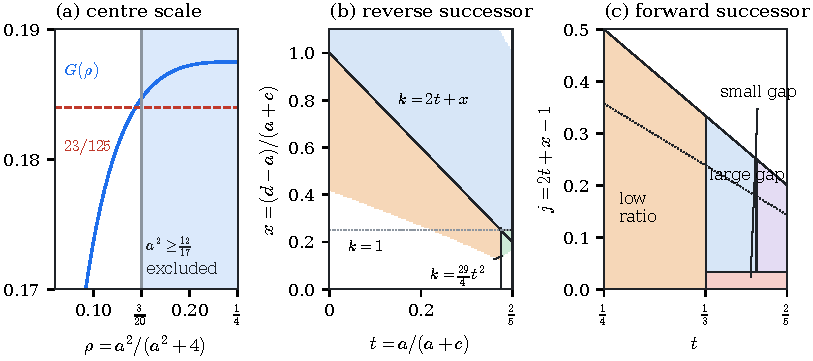
\includegraphics[width=\textwidth]{figures/fig-mixed-domains.pdf}
\caption{Parameter bounds for class $\cls{M2}$. (a)~The lower bound
$G(\rho)=(9/4-B(\rho)^2)/(16(1-\rho)^2)$ for the Casimir at a reverse centre, with
$\rho=a^2/(a^2+4)$. It exceeds the cap $23/125$ (dashed) on $[3/20,1/4)$, which proves
$a^2<12/17$ (\cref{lem:m2-scale}).
(b)~The parameters $(t,x)$ of the scalar reverse exclusion (\cref{prop:m2-reverse-core}), below
$x=1.1$, by the face to which $k$ is lowered: the unit shape $k=1$, the order face $k=2t+x$, and
the scale strip $k=29t^2/4$, which lies in $13/35<t<2/5$, $x\le9/35$. Points above $x=1$ belong to
the order face. (c)~The parameters $(t,j)$ of a forward successor, in $1/4<t<2/5$, $0<j<1-2t$: the
low ratio $t\le1/3$, the two large-gap regions $j\ge1/30$, split at $t=3/8$, and the small-gap
region, where the Casimir exceeds the cap. The dotted line is $j=\frac57(1-2t)$.}\label{fig:m2-domains}
\end{figure}

\subsubsection{The minimum is a reverse centre}\label{sec:m2-centre}

\begin{proposition}[The minimum is a reverse centre]\label{prop:m2-centre}
Let $P$ be a competitive normal vertex period of class $\cls{M2}$ with at least six pieces. There is
an index $m$ with $a_m\le a_k$ for every $k$ such that the switches $m-1$ and $m$ are reverse and the
switches $m-2$ and $m+1$ are forward.
\end{proposition}

Let $a_m$ be a smallest active margin of the period; the active margins are periodic, so a minimum
exists. A minimum cannot be at a turn: at three pieces with labels $i,j,i$ the active margins are
strictly log-concave, $a_{k}a_{k+2}<a_{k+1}^2$ (\cref{lem:three-arc}), so the middle one is not the
smallest of the three. If both switches at $m$ are reverse, $m$ is the centre of a reverse run. The
remaining case, both switches forward, is excluded by the following theorem, which uses only
stationarity and the floors that the two missing controls impose.

\begin{proposition}[No small forward minimum]\label{prop:m2-small-forward}
Let $P$ be a normal vertex period with at least three pieces, and let $m$ be an index such that the
switches $m-2,m-1,m,m+1$ are forward, $a_m\le a_j$ for $m-2\le j\le m+2$, and $a_m^2\le4/3$. This is
impossible.
\end{proposition}

The proof writes the multiplier in the frame of
the central piece, eliminates one coordinate with stationarity at the centre, and keeps the
stationarity row at the smaller neighbour with the two exterior floors $v\ge F_x(q)$ at the forward
switches. The remaining face is a one-variable residual with an exactly controlled second
derivative; two integrations and the Pad\'e bound $\frac12(h-h^{-1})-\log h\ge (h-1)^3/(3h(h+1))$
leave a rational expression, negative by an elementary cubic comparison. No Casimir bound is used.

\begin{proof}[Proof of \cref{prop:m2-centre}]
Take a global minimum $m$. If exactly one of the switches $m-1,m$ is reverse, the pieces $m-1,m,m+1$
have labels $i,j,i$, and \cref{lem:three-arc} contradicts minimality. If both are forward, the
strict centre minimum of the neighbouring reverse runs (\cref{prop:run-structure}) forces the
switches $m-2$ and $m+1$ to be forward as well: otherwise the centre of the adjacent reverse run
would have a smaller active margin. The period is mixed, so it has a reverse centre; by
\cref{lem:m2-scale} its active margin squared is below $12/17$, hence $a_m^2<12/17<4/3$, and
\cref{prop:m2-small-forward} gives a contradiction. If both switches are reverse, they form a
maximal reverse run, of length two in class $\cls{M2}$, and $m$ is its centre.
\end{proof}

\subsubsection{Orientation by reflection}\label{sec:m2-reflection}

Let $S=\mathrm{diag}(1,-1)$. Reflecting the plane and reversing time is a symmetry of the control
problem: it maps a normal vertex period to another one with the same cost, and reverses the order of
the pieces.

\begin{lemma}[Reflection]\label{lem:m2-reflection}
For every normal vertex period $P$ there is a normal vertex period $P'$ with the same number of
pieces and the same cost, whose state stays in $\hstarstar$ when that of $P$ does, with labels
$i'_k=c-i_{-1-k}$ for a constant $c\in\Z/3$ and active margins $a'_k=a_{-1-k}$. Its switch $k$ is
forward if and only if the switch $-2-k$ of $P$ is forward, and $P'$ is of class $\cls{M2}$ when $P$
is.
\end{lemma}

The construction is $u'(t)=\varsigma u(T-t)$, with $\varsigma$ the permutation of the vertices that
reflects the labels, $g'(t)=SR^{-1}g(T-t)S$, $X'(t)=-SX(T-t)S$, and $\Lambda'(t)=-S\Lambda(T-t)S$ for
both costates. Since $SJS=-J$, the cost density is preserved, and $\hstarstar$ is symmetric under
$x\mapsto-x$. Reading the signs in reverse order does not negate them: a reverse switch of $P$
is a reverse switch of $P'$.

By \cref{prop:m2-centre,lem:m2-reflection} we may assume that the global minimum $a=a_m$ is a
reverse centre and that the turn after it is the smaller one: $a_{m+1}\le a_{m-1}$. (At a tie either
choice works.) After relabeling the vertices by a power of $R$, which changes neither the cost nor
the active margins, the pieces $m-2,\dots,m+3$ have labels and active margins
\begin{equation}\label{eq:m2-labels}
0(p),\quad 1(b),\quad 0(a),\quad 2(c),\quad 0(d),\quad 1(r)
\end{equation}
when the switch $m+2$ is forward.
These are consecutive pieces of the period, continued through the twisted seam when necessary; they
need not be distinct from other pieces named later, and they are not a closed competitor.

\subsubsection{The nonshort window}\label{sec:m2-window}

\begin{table}[t]
\centering\small
\begin{tabular}{@{}l>{\raggedright\arraybackslash}p{0.74\textwidth}@{}}
\toprule
Symbol & Meaning (in \cref{sec:mixed} and \cref{app:nonshort-estimates})\\
\midrule
$p,b,a,c,d,r$ & active margins of six consecutive pieces \eqref{eq:m2-labels}; $a$ is a global
minimum, and $c\le b$\\
$K_a,\ Q,\ K_r$ & $a^2+4$, $d^2+4$, $r^2+4$\\
$S,T,W,Z,Y$ & $a+b$, $a+c$, $c+d$, $d+r$, $W^2-T^2$ (here $T$ is not the terminal time)\\
$u,v,w$ & eight times the norms of the switches $b\to a$; $a\to c$ and $c\to d$; $d\to r$\\
$h_a,h_d$ & the diagonal entries of the multiplier in the frames of the pieces $a$ and $d$\\
$U(x),\ g_B(x)$ & $1-x+x^2$ and $(B^2+Bx+x^2)/(B+x)^2=1-Bx/(B+x)^2$\\
$\operatorname{Sec}(A,B,P)$ & the average of $g_B$ over the interval between $A$ and $P$\\
$F_x(q)$ & $1+x^2q-xq\log q/(q-1)$, with $F_x(1)=U(x)$\\
$t,x,k,q$ & $a/T$, $(d-a)/T$, $K_a/T^2$, $WZ/Q$ (normalized coordinates)\\
$j$ & $2t+x-1$, the gap of a forward successor\\
\bottomrule
\end{tabular}
\caption{Local notation of class $\cls{M2}$. The letters $p,r,t,u,x$ have their usual meaning
elsewhere in the paper.}\label{tab:m2-notation}
\end{table}

\Cref{tab:m2-notation} lists the local notation. All quantities in the window come from the one
normal multiplier of the period. The factors of the same-sign pieces follow from the one-arc map
(\cref{lem:one-arc}) and the margins $(a_k,a_{k+1},(4-a_ka_{k+1})/(a_k+a_{k+1}))$ of the state at a
switch: the factor of a piece with incident signs $++$, $--$, $-+$, $+-$ is $s_{k-1}s_k/K_k$,
$K_k/(s_{k-1}s_k)$, $s_k/s_{k-1}$, $s_{k-1}/s_k$ respectively. In the window this gives
the central factor $K_a/(ST)>1$, the factor $q=WZ/Q>1$ of the piece $d$, and $d>a$ from the turn
$c$.

Both switches at a turn have the same norm, the turn secant (\cref{lem:switch-norms}):
$u=\operatorname{Sec}(a,b,p)$ and $v=\operatorname{Sec}(a,c,d)$, where
\[
\operatorname{Sec}(A,B,P)=1+\frac{B^2}{(A+B)(P+B)}-\frac{B}{P-A}\log\frac{P+B}{A+B}.
\]
In the frame of the central piece the multiplier is
\begin{equation}\label{eq:m2-Ua}
U_a=\begin{pmatrix}h_a&-K_a^2v/(8S^2)\\ S^2u/8&-h_a\end{pmatrix},\qquad
\gamma^2=\det U_a=\frac{uvK_a^2}{64}-h_a^2,
\end{equation}
and stationarity at the centre (\cref{lem:stationarity}) fixes the diagonal:
\begin{equation}\label{eq:m2-ha}
\begin{gathered}
h_a=\frac{K_a}{16a}\bigl(Su+Tv-C(b,a,c)\bigr),\\
C(p,a,n)=p+a+n-\frac{a^2}{p+a}-\frac{a^2}{a+n}+\frac{a^3}{a^2+4}
-a\log\frac{(p+a)(a+n)}{a^2+4}.
\end{gathered}
\end{equation}
Here $C(p,a,n)$ is four times the partial derivative of the normalized cost $\cost/\sqrt{12}$ in
the active margin of a same-sign piece. Transport across the centre and the turn to the frame of
the piece $d$ gives
\begin{equation}\label{eq:m2-transport}
h_d=h_a+\frac{vY}{8},\qquad w=\frac{uK_a^2+16h_aY+vY^2}{Q^2},
\end{equation}
and stationarity at $d$, the first piece of the forward run after the turn, is the root equation
\begin{equation}\label{eq:m2-root}
R_d:=C(c,d,r)-Wv-Zw+\frac{16\,d\,h_d}{Q}=0.
\end{equation}

\begin{proposition}[The nonshort window]\label{prop:m2-window}
Let $P$ be competitive, with state in $\hstarstar$, of class $\cls{M2}$ and with at least six pieces;
let $m$ be as in \cref{prop:m2-centre} with $a_{m+1}\le a_{m-1}$, and let the switch $m+2$ be
forward. Then $(p,b,a,c,d,r)=(a_{m-2},\dots,a_{m+3})$, with $u,v,h_a,w$ as above, satisfy:
\begin{enumerate}[label=(\roman*)]
\item the order $a<b$, $a<c\le b$, $a<p$, $a<d$, $a\le r$;
\item strict star at the five switches, $pb,ab,ac,cd,dr<4$; the factors $ST<K_a$ and $Q<WZ$;
three-arc log-concavity $ad<c^2$;
\item the compact domain: $a\ge2/15$, $cd+\frac2{15}(c+d)\le4$, $dr+\frac2{15}(d+r)\le4$,
$d,r\le8$, and $a+c,\,c+d,\,d+r\ge\frac12$; and the scale bound $a^2<12/17$;
\item the turn secants $u=\operatorname{Sec}(a,b,p)$, $v=\operatorname{Sec}(a,c,d)$; the switching
inequalities $g_b(p)\le u\le g_b(a)$, $g_c(d)\le v\le g_c(a)$, $w\ge g_d(r)$; the missing-control
floors $v\ge F_{d/W}(q)$ and $w\ge F_{d/Z}(q)$;
\item the identities \eqref{eq:m2-ha}, \eqref{eq:m2-transport} and \eqref{eq:m2-root};
\item $27/256<uvK_a^2/64-h_a^2<9193/50000$.
\end{enumerate}
\end{proposition}

\begin{proof}[Sketch]
Each item is read off the costate cycle at the switches of the window: (i) from minimality, the
choice $c\le b$ and \cref{prop:run-structure}; (ii) from the margin transports (\cref{lem:one-arc});
(iii) from \cref{thm:compact-domain} at the switching times (every margin is at least $2/15$, and
$y\le9/2$ on $\hstarstar$ gives the pair sums and $d,r\le8$) and \cref{lem:m2-scale}; (iv) from
\cref{lem:switch-norms} and, for the floors, from $H_i\le0$ for the two controls missing at a forward
switch, written through stationarity, an identity algebraic in
$x$ that holds for every $x$; (v) from exact transports; (vi) from \cref{lem:m2-casimir}.
\end{proof}

\subsubsection{The successor of the forward piece}\label{sec:m2-continuation}

The window does not yet contain a contradiction: the root equation \eqref{eq:m2-root} has solutions
compatible with (i)--(vi). The next actual switch, after the piece $r$, supplies one more condition.
Finiteness of the representation guarantees that it exists, and equal neighbouring labels have
been merged, so it is forward or reverse. Let
\[
t_{\mathrm{next}}=\frac{Q^2v-16h_dZ^2+wZ^4}{K_r^2}
\]
be the norm of that switch when it is forward, read in the frame of the piece $r$.

\begin{proposition}[The continuation alternative]\label{prop:m2-continuation}
In the situation of \cref{prop:m2-window}:
\begin{enumerate}[label=(\alph*)]
\item if the switch $m+3$ is forward, to a piece with active margin $s$, then $s\ge a$, $rs<4$,
$K_r<Z(r+s)$, $t_{\mathrm{next}}\ge g_r(s)\ge\frac34$, and both missing-control floors hold at the
piece $r$;
\item if the switch $m+3$ is reverse, to a piece with active margin $A$, then $a\le A<d$, $Ad<r^2$,
$w=\operatorname{Sec}(A,r,d)$ and $w\le g_r(A)$.
\end{enumerate}
\end{proposition}

In (a) the inequality for $t_{\mathrm{next}}$ is the forward switching inequality at the piece $r$,
whatever the margin $s$ and the length of the forward run. In (b) the piece $r$ is a turn, both its
switches have the norm $\operatorname{Sec}(A,r,d)$, $A\ge a$ by minimality, and $Ad<r^2$ is
three-arc log-concavity. Since $g_r$ decreases on $(0,r)$ and $A<r$, extending the average from
$[A,d]$ to $[a,d]$ also gives $w\le\operatorname{Sec}(a,r,d)$; we use (b) as stated.

\subsubsection{The boundary comparison and the residual}\label{sec:m2-comparison}

The root equation \eqref{eq:m2-root} is affine in the incident norm $u$, with slope
\begin{equation}\label{eq:m2-Ru}
\partial_uR_d=\frac{K_a}{aQ^2}\bigl(dSQ-Z(aK_a+SY)\bigr)<0,
\end{equation}
negative because $Y>0$, $Z>Q/W$, and $dSQ-Z(aK_a+SY)<(Q/W)\{a(ST-K_a)+Sc(a-d)\}<0$. The reverse
switch $b\to a$ caps $u$ by the ceiling $U(a/S)=g_b(a)$, so the actual data satisfy
$R_d(U(a/S))\le R_d(u)=0$. Stationarity at $d$ thus imposes an upper bound on the incident norm. On the necessary domain,
we will show that stationarity instead requires the norm to exceed this ceiling.

Before testing this, we remove the margins $b$ and $p$. Keep $a,c,d,r$ and the actual $v$ fixed and
raise $b$ to $b_*=K_a/T-a$, the value at which the central factor $K_a/(ST)$ equals one. Write
$G(b)=R_d(U(a/(a+b));b)$ for the residual at the ceiling, with $h_a$ given by central stationarity at
the margin $b$.

\begin{lemma}[Boundary comparison]\label{lem:m2-comparison}
For the window of \cref{prop:m2-window}, $G(b_*)<0$; the root $u_*$ of $R_d(\,\cdot\,;b_*)=0$
satisfies $u_*<U(aT/K_a)$; and the outgoing norm $w_*$ of that boundary root satisfies $w_*<w$.
\end{lemma}

\begin{proof}
Along $[b,b_*]$ the derivative is $G'(b)=\partial_uR_d\cdot a(b-a)/(a+b)^3<0$, and at the actual
margin $G(b)=\partial_uR_d\,(U(a/S)-u)\le0$, so $G(b_*)<0$. Along the curve of roots $u(b)$, the
outgoing norm has $dw/db=dK_a^3G(b)/(aQ^3(\partial_uR_d)^2)<0$, so $w$ decreases from its actual
value.
\end{proof}

This is a scalar comparison: the point $b_*$ need not belong to a trajectory, and no switching
inequality, floor or Casimir bound is transported to it.

At $b_*$ the logarithm of the centre disappears ($C(b_*,a,c)=4/T+4c/K_a$), and homogeneity lets us
normalize by $T=a+c$. In the coordinates $t=a/T$, $x=(d-a)/T$, $k=K_a/T^2$, $q=WZ/Q$, write
$W=1+x$, $p=t+x$ and $B=k+2tx+x^2$ for the normalized values; the margins are recovered from
$(t,x,k,q)$, since $a^2(k-t^2)=4t^2$. The positive multiple
\[
N(t,x,k,q,v,\log q)=t\,B\,q\,W\cdot\frac{G(b_*)}{T}
\]
is a polynomial in $t,x,k,q,v$ and $L=\log q$, affine in $k$, in $v$ and in $L$; \cref{app:m2-residual} gives its coefficients. The normalized
incoming secant is $v=\operatorname{Sec}(t,1-t,t+x)=1+(1-t)^2/W-(1-t)\log W/x$.

\begin{lemma}[Shape monotonicity]\label{lem:m2-shape}
If $0<t<1$, $x>0$, $q\ge1$, $v\le U(t)$ and $L<q-1$, then $N(t,x,k,q,v,L)$ is nondecreasing in $k$.
\end{lemma}

The coefficient of $k$ is at least $q\,t\,x(1-t)\{(q-1)(2x+1)+tx\}>0$ (\cref{app:m2-residual}).
Since $k$ moves with $a$ at fixed $t$, the lemma lets every later argument lower $k$ to the smallest
value that the necessary conditions allow, and prove $N>0$ there.

\begin{lemma}[Necessary conditions]\label{lem:m2-necessary}
Every window of \cref{prop:m2-window} satisfies
\begin{enumerate}[label=(\roman*)]
\item $0<t<\frac12$, $x>0$, $k>1$, $1<q<W/p$, $v=\operatorname{Sec}(t,1-t,t+x)$,
$1-(1-t)p/W^2\le v\le U(t)$ and $F_{p/W}(q)\le v$;
\item $N(t,x,k,q,v,\log q)<0$;
\item $t<2/5$;
\item $a<4/5$, that is, $k>29t^2/4$;
\item $d^2+2cd>4$, that is, $k<2t+2x+x^2$;
\item $3d<7c$, that is, $x<\frac73-\frac{10}3t$;
\item if the successor is reverse, $d\le b_*$, that is, $k\ge2t+x$.
\end{enumerate}
\end{lemma}

Item (i) restates the window ($k>1$ is $ST<K_a$ with $S\ge T$, and $q<W/p$ is $dr<4$); the
others are proved in \cref{app:m2-bounds}.

\subsubsection{The reverse successor}\label{sec:m2-reverse}

\begin{proposition}[The scalar reverse exclusion]\label{prop:m2-reverse-core}
Let $0<t<2/5$, $x>0$, $\max\{1,\,2t+x,\,29t^2/4\}\le k<2t+2x+x^2$, $x<\frac73-\frac{10}3t$,
$1<q<(1+x)/(t+x)$, $v=\operatorname{Sec}(t,1-t,t+x)\le U(t)$ and $F_{(t+x)/(1+x)}(q)\le v$.
Then $N(t,x,k,q,v,\log q)>0$.
\end{proposition}

\begin{proof}
By \cref{lem:m2-shape} it suffices to find a shape $k'\le k$ allowed by the hypotheses with
$N(k')>0$. There are three exhaustive cases (\cref{fig:m2-domains}(b)).
\begin{enumerate}[label=(\arabic*)]
\item If $t\le13/35$ and $x\le1-2t$, lower $k$ to $1$, where $N(1)>0$ (\cref{lem:m2-unit-shape}).
\item If $2t+x\ge1$ and $x>1/4$, lower $k$ to the order face $k=2t+x$. The floor and the swapped
secant order give $q\le(1+x)/(2t+x)$. On this face $N$ is a positive
multiple of a function $\alpha+\beta q+\gamma/q-p\log q$, concave in $q$, so it suffices to check
$q=1$ and the upper end, where it is positive (\cref{lem:m2-order-face}).
\item Otherwise $13/35<t<2/5$ and $x\le9/35$; lower $k$ to the scale face $k=29t^2/4$, where
$N>0$ (\cref{lem:m2-strip}).\qedhere
\end{enumerate}
\end{proof}

On each face the logarithms are first replaced by rational bounds with the correct signs ($v$ by a
larger $\bar v$, $\log q$ by $L_+(q)\ge\log q$, the floor by a smaller $F_\ell$), which lowers $N$; the
result is a cubic in $y=q-1$ whose positivity for $y\ge0$ follows from six polynomial signs in
$(t,x)$. \Cref{app:m2-reverse-signs} gives the reduction and proves the signs.

\begin{theorem}[Reverse successor]\label{thm:m2-reverse}
No window of \cref{prop:m2-window} has a reverse successor.
\end{theorem}

\begin{proof}
By \cref{prop:m2-continuation}(b) and \cref{lem:m2-necessary}, the normalized window satisfies every
hypothesis of \cref{prop:m2-reverse-core}, which gives $N>0$, against \cref{lem:m2-necessary}(ii).
\end{proof}

\subsubsection{The forward successor}\label{sec:m2-forward}

When the successor is forward the order bound (vii) fails, and the residual alone does not suffice.
Two facts replace it. First, the scalar reverse exclusion applies to every window with $k\ge2t+x$,
without any assumption on the successor, so every window has the opposite order
\begin{equation}\label{eq:m2-order}
k<2t+x,\qquad\text{equivalently } d>b_*\text{ and } j=2t+x-1>0.
\end{equation}
Second, the forward successor gives a lower bound for the next norm at the
boundary root. Both the actual point and the boundary point satisfy the root equation
\eqref{eq:m2-root}, which makes $h_d$ an affine function of $w$; on that line the next norm is a
decreasing affine function of $w$, and $w_*<w$, so the next norm $t_{\mathrm{next},*}$ at the
boundary is at least $t_{\mathrm{next}}\ge\frac34$. As a function of the
incident norm the next norm is affine, and its value at the root differs from its value
$\mathcal T_U$ at the ceiling by a multiple of $N$. For multipliers $\alpha>0$ and $M\ge0$ the
combined residual
\begin{equation}\label{eq:m2-comb}
\begin{aligned}
\mathcal H&=\alpha N+C_*\bigl(\tfrac34-t_{\mathrm{next},*}\bigr)+M\bigl(F_{p/W}(q)-v\bigr)\\
&=(\alpha+1-Je^2)N+C_*\bigl(\tfrac34-\mathcal T_U\bigr)+M\bigl(F_{p/W}(q)-v\bigr),
\end{aligned}
\end{equation}
with $e=q/W$, $J=t+x(x+2)$ and an explicit $C_*>0$, is therefore negative at every window with a
forward successor. It is affine in $v$, in $\log q$ and in the floor value,
and a concave quadratic in $k$.

The unit face of the low-scale argument gives $t>1/4$ (\cref{lem:m2-low-unit}); with the
derivative floor $v\ge g_c(d)$ this gives $x<1$ and $4t+x<2$, and a quantitative form of the swapped
secant order gives $q<W/(1+2j)$. The remaining parameters are cut down in
three steps (\cref{fig:m2-domains}(c)).

\begin{proposition}[The forward successor in three steps]\label{prop:m2-forward-steps}
Every window of \cref{prop:m2-window} with a forward successor satisfies
\begin{enumerate}[label=(\alph*)]
\item $t>1/3$;
\item $j=2t+x-1<1/30$;
\end{enumerate}
and then the Casimir of the period is at least $9193/50000$, against \cref{lem:m2-casimir}(b).
\end{proposition}

\begin{proof}[Outline]
(a) If $t\le1/3$, take $\alpha=6$ and $M=0$. The coefficients of $v$ and of $\log q$ in $\mathcal H$
are negative, so raising $v$ to a rational majorant $\hat v$ and $\log q$ to $L_+(q)$ keeps
$\mathcal H$ negative. The result increases in $k$, so it is negative at $k=1$ as well; but at
$k=1$ it is positive (\cref{lem:m2-low-ratio}).

(b) Suppose $j\ge1/30$. Then $1/3<t<2/5$ by (a), and the derivative floor in integral form gives
$j<\frac57(1-2t)$. For $1/3\le t\le3/8$ take $\alpha=\frac72-10(q-1)$ and $M=8j+8(q-1)-\frac16$,
both positive here; after the substitutions of $v$, $\log q$ and the floor by rational bounds, the
residual increases in $k$ and is positive at $k=1$. For $3/8\le t<2/5$ take $\alpha=4$ and $M=1$;
the residual increases in $k$ and is positive at the scale face $k=29t^2/4$
(\cref{lem:m2-large-gap}).

(c) Now $1/3<t<2/5$, $0<j<1/30$ and $1\le k<31/30$. With $N<0$, a rational comparison in $q$ gives
$\chi=pq/W>4/7$ (\cref{lem:m2-chi}). On the stationarity line of the piece $d$, the diagonal $h_d$
is an affine function $H_d(w)$ of the outgoing norm, and the Casimir is
$\Gamma(w)=(4B^2vw-H_d(w)^2)/(16(k-t^2)^2)$ in normalized form. For
$w\ge3/4$ one has $\Gamma'(w)<0$ (\cref{lem:m2-slope}). The actual $w$ lies between $3/4$ and the
central upper envelope $w_U$, the transported norm with $u$ at its ceiling and $b=b_*$, so $\gamma^2=\Gamma(w)>\Gamma(w_U)$. At $w_U$ the event factor $q$ is
eliminated with the floor (\cref{lem:m2-qelim}), and the remaining function of $(t,x,k,v)$
exceeds $9193/50000$ (\cref{lem:m2-envelope}).
\end{proof}

\begin{theorem}[Forward successor]\label{thm:m2-forward}
No window of \cref{prop:m2-window} has a forward successor.
\end{theorem}

This is \cref{prop:m2-forward-steps}. The obstruction in its last step is the cost itself: the turn
data force the Casimir of the period above $9193/50000$, and by \cref{lem:m2-casimir}(a) a period
with such a Casimir costs more than $\Aoct$.

\begin{remark}[Small scale]\label{rem:m2-low-scale}
The same methods exclude every window with $a\le\frac12$, whatever the sign of the successor:
then $k\ge17t^2$, and
$N$ can be lowered to $k=1$ or to $k=2t+\frac12$. The proof above needs only the unit face of that
argument (\cref{lem:m2-low-unit}), which gives $t>1/4$.
\end{remark}


\subsubsection{Proof of \texorpdfstring{\cref{thm:class-M2}}{the theorem for class M2}}\label{sec:m2-proof}

Let $P$ be as in \cref{thm:class-M2}, and take $m$ from \cref{prop:m2-centre}. If $a_{m+1}>a_{m-1}$,
replace $P$ by its reflection (\cref{lem:m2-reflection}): it is again competitive, of class
$\cls{M2}$, with state in $\hstarstar$ and the same number of pieces; the minimum moves to $-1-m$,
the four switches around it keep their signs in reverse order, and the smaller turn now follows the
centre. If the switch $m+2$ after the turn is reverse, the seven pieces $m-2,\dots,m+4$ form a
smaller-short window, excluded by \cref{thm:m2-smaller-short}. If it is forward, \cref{prop:m2-window} gives a nonshort window,
and \cref{prop:m2-continuation} gives a forward or a reverse successor; \cref{thm:m2-forward}
and \cref{thm:m2-reverse} exclude them. \qed

\subsection{Estimates for class M2: the nonshort cases}\label{app:nonshort-estimates}

This subsection proves the scalar inequalities behind \cref{sec:mixed}, in the notation of
\cref{tab:m2-notation}. Every step concerns explicit functions of at most five real variables.
The logarithm estimates follow from one reciprocal integral, using Jensen's inequality and
pointwise bounds on the integrand. They give bounds for the secants and the duration. The
remaining face arguments reduce polynomial signs, one variable at a time, to inequalities on
intervals. Several of these polynomials are long; they are determined by the displayed
definitions, and we state the identities and bounds on which each sign rests.

\subsubsection{Secants and floors}\label{app:m2-secants}

For $B>0$ the function $g_B(x)=1-Bx/(B+x)^2$ decreases on $(0,B)$, increases on $(B,\infty)$, and
has minimum $g_B(B)=3/4$; also $g_B(x)=U(B/(B+x))=U(x/(B+x))$. The turn secant
$\operatorname{Sec}(A,B,P)=(P-A)^{-1}\int_A^Pg_B$ has the antiderivative
$s-B\log(B+s)-B^2/(B+s)$.

\begin{lemma}[Secants]\label{lem:m2-secants}
\begin{enumerate}[label=(\alph*)]
\item If $0<a\le c<d$, then $\operatorname{Sec}(a,c,d)<\operatorname{Sec}(a,d,c)$.
\item If $0<c\le d$, then $z\mapsto\operatorname{Sec}(z,d,c)$ strictly decreases on $(0,c]$.
\item For $P,C>0$ and $q>1$, $F_{P/(P+C)}(q)=\operatorname{Sec}((P+C)/q-P,\,P,\,C)$. In particular
$F_{d/W}(q)=\operatorname{Sec}(B_0,d,c)$ with $B_0=(4-dr)/(d+r)$, the third margin at the switch
$d\to r$.
\item If $ad<c^2$, then $\operatorname{Sec}(a,c,d)<\frac12(g_c(a)+g_c(d))$.
\item If $0<A<P$, $B>0$ and $B/(A+B)\ge3/5$, then $\operatorname{Sec}(A,B,P)>\mu_*:=(2\sqrt{130}-4)/25$.
\end{enumerate}
\end{lemma}

\begin{proof}
(a) $\operatorname{Sec}(a,d,c)=\int_0^1g_1(u)\,d\theta$ and $\operatorname{Sec}(a,c,d)=\int_0^1g_1(v)\,d\theta$
with $u=(a+\theta(c-a))/d$ and $v=(a+\theta(d-a))/c$. Here $v>u$, $uv<1$, and
$g_1(u)-g_1(v)=(v-u)(1-uv)/((1+u)^2(1+v)^2)>0$.
(b) The derivative is $(\operatorname{Sec}(z,d,c)-g_d(z))/(c-z)$, and the average of the decreasing
function $g_d$ over $[z,c]$ is below its value at $z$.
(c) Substitute $(P+C)/q-P$ in the closed form of the secant; $W/q-d=Q/Z-d=B_0$.
(d) For $a\le x\le d$,
\begin{multline*}
\frac{(d-x)g_c(a)+(x-a)g_c(d)}{d-a}-g_c(x)\\
=\frac{c(x-a)(d-x)\,[c^2(a+d+2c)+(c^2-ad)x]}{(a+c)^2(d+c)^2(x+c)^2}\ge0;
\end{multline*}
integrate over $[a,d]$.
(e) With $\eta=B/(A+B)$ and $q=(P+B)/(A+B)>1$, the secant is
$1+\eta^2/q-\eta\log q/(q-1)$. The upper bound of \cref{lem:m2-logs}(b) gives
\[
 \operatorname{Sec}(A,B,P)>
 1-\frac\eta6+\frac{a}{q}-\frac{b}{q+1},\qquad
 a=\eta\left(\eta-\frac16\right),\quad b=\frac{4\eta}{3}.
\]
For $a,b>0$, completing a square gives
\[
 \frac{a}{q}-\frac{b}{q+1}+(\sqrt b-\sqrt a)^2
 =\frac{\bigl(\sqrt a(q+1)-\sqrt b\,q\bigr)^2}{q(q+1)}\ge0.
\]
Thus the secant exceeds
\[
 m(\eta)=1-\eta^2-\frac{4\eta}{3}+\frac{2\eta}{3}\sqrt{12\eta-2}.
\]
This lower bound increases on $1/2\le\eta\le1$. Indeed, with
$w=\sqrt{12\eta-2}-2$, it is $3/4+w^2(4-w^2)/144$, and $0\le w^2<2$ on that interval.
For $\eta\ge3/5$ we obtain
$\operatorname{Sec}(A,B,P)>m(3/5)=\mu_*$.
\end{proof}

\subsubsection{Rational bounds for the logarithms}\label{app:m2-logs}

\begin{lemma}[Logarithms]\label{lem:m2-logs}
Let $0<t<1$, $x>0$, $q>1$, $c=1-t$, $W=1+x$, $X=x+2$, $p=t+x$, $g=1-cp/W^2$, and let
$v=1+c^2/W-c\log W/x$ be the normalized incoming secant.
\begin{enumerate}[label=(\alph*)]
\item $\log(1+x)>2x/X+2x^3/(3X^3)$; hence $v<\bar v=1+c^2/W-(2c/X)(1+x^2/(3X^2))$.
\item $\log q<L_+(q)=(q-1)(q^2+10q+1)/(6q(q+1))$; hence
$F_{p/W}(q)>F_\ell=1+p^2q/W^2-(p/W)(q^2+10q+1)/(6(q+1))$.
\item With $\tau=x/X$,
$\log(1+x)>L_J(x):=2\tau\bigl(1+\tau^2/[3(1-3\tau^2/5)]\bigr)$; hence
$v<v_G=g+(cx/W^2)(T_G(x)-t)$ with $T_G=(90-19x^2)/(12(x^2+10x+15))$.
\item $\log(1+x)>3x(x+2)/(x^2+6x+6)$; hence $v<V=1+c^2/W-3c(x+2)/(x^2+6x+6)$.
\item $\bar v-g=((1-t)x/W^2)(T(x)-t)$ with $T(x)=(-2x^3-x^2+10x+12)/(3(x+2)^3)$; so $v\ge g$ forces
$t<T(x)$. The function $T$ decreases, and $T(1)=19/81<1/4$.
\end{enumerate}
\end{lemma}

\begin{proof}
All the logarithm bounds follow from the reciprocal integral
\[
 \log\frac{1+\tau}{1-\tau}=2\tau I(\tau),\qquad
 I(\tau)=\int_0^1\frac{\dd s}{1-\tau^2s^2}\qquad(0<\tau<1).
\]
For (a), the integrand exceeds $1+\tau^2s^2$. For (b), it is less than
$1+\tau^2s^2/(1-\tau^2)$ for $0<s<1$. Integration gives
$I(\tau)<1+\tau^2/[3(1-\tau^2)]$; at $\tau=(q-1)/(q+1)$ this is the displayed upper bound.

For (c), write
$I(\tau)=1+\tau^2\int_0^1s^2/(1-\tau^2s^2)\,\dd s$.
Apply strict Jensen to $y\mapsto(1-\tau^2y)^{-1}$ with probability density $3s^2$.
The mean of $s^2$ is $3/5$, giving $I(\tau)>1+\tau^2/[3(1-3\tau^2/5)]$.
As $c>0$, this implies $v<v_J:=1+c^2/W-cL_J(x)/x$. The required ceiling follows from
\[
 v_G-v_J=\frac{cx^6}{12W^2(x+2)(x^2+10x+10)(x^2+10x+15)}>0.
\]
For (d), Jensen with uniform measure gives $I(\tau)>1/(1-\tau^2/3)$.
The resulting logarithm bound also has the direct verification
\[
 \frac{\dd}{\dd x}\left(\log(1+x)-\frac{3x(x+2)}{x^2+6x+6}\right)
 =\frac{x^4}{(1+x)(x^2+6x+6)^2}>0;
\]
the difference vanishes at $x=0$. Part (e) follows by subtraction and
$T'(x)=-(11x^2+24x+16)/(3(x+2)^4)$.
\end{proof}

\subsubsection{The residual}\label{app:m2-residual}

Put $c=1-t$, $p=t+x$, $W=1+x$, $Y=x(x+2)$, $B=k+2tx+x^2$, $Z=qB/W$ (the normalized $d+r$), and
\[
H_0=\frac kt\,(v-1+t^2)+t(2-t),\qquad w_U=\frac{k^2-kt+t^2+H_0Y+vY^2}{B^2},
\]
the central diagonal and the transported outgoing norm with the incident norm at the boundary
ceiling $U(t/k)$. The root function at the ceiling, divided by $T$, is
\[
R=c+Z-\frac{p^2}{W}-\frac{p^2}{Z}+\frac{p^3}{B}-p\log q-Wv-Zw_U+\frac{p(H_0+2vY)}{B},
\]
and $N=tBqW\,R$. Clearing denominators cancels every negative power, and $N$ is a polynomial,
affine in $k$, $v$ and $L=\log q$:
\begin{itemize}
\item the coefficient of $v$ is $N_v=-xq\,I$ with
$I=k+tx+tW(k-2t)+(q-1)\bigl(kX+txX^2\bigr)$, nonpositive when $k\ge2t$;
\item the coefficient of $L$ is $N_L=-tpqWB\le0$;
\item the coefficient of $k$ is
\begin{multline*}
A=q\bigl\{x[(1-v)(1+tW)-t(1-t^2)]\\
+(q-1)[t^2(1+2x-x^2)+2tx^2+(1-v)Y]-tpW L\bigr\}.
\end{multline*}
\end{itemize}
In $A$ the coefficient of $v$ is $-qx[(q-1)(x+2)+1+tW]<0$ and that of $L$ is $-qtpW<0$. Inserting
$v\le U(t)=1-t+t^2$ and $L<q-1$ and collecting gives
$A>q\,t\,x(1-t)[(q-1)(2x+1)+tx]>0$, which is \cref{lem:m2-shape}.

\begin{lemma}[Rational relaxation]\label{lem:m2-relax}
If $k\ge2t$, $q>1$ and $F_{p/W}(q)\le v$, then
\[
N(v,\log q)\ \ge\ N(\bar v,L_+)-(q-1)(\bar v-F_\ell),
\]
and $P_k:=6(q+1)W^2X^3\{N(\bar v,L_+)-(q-1)(\bar v-F_\ell)\}$ is a polynomial in $t$, $x$, $k$ and
$y=q-1$, cubic in $y$.
\end{lemma}

\begin{proof}
$N_v\le0$, $N_L\le0$, $v<\bar v$ and $\log q<L_+$, while $F_\ell<F_{p/W}(q)\le v<\bar v$ makes the
subtracted term nonnegative.
\end{proof}

\subsubsection{The necessary bounds}\label{app:m2-bounds}

We prove \cref{lem:m2-necessary}(iii)--(vii).

\runin{The scale.} At the centre, \eqref{eq:m2-centre} holds with $u_{\mathrm i}=u$,
$u_{\mathrm o}=v$, $r=a/S$ and $t=a/T$. Lowering both norms to a floor $\mu$ and raising both ratios
to a cap $\zeta$ gives $\gamma^2\ge(4\mu^2-B(\rho)^2)/(16(1-\rho)^2)$ with
$B(\rho)=1-\rho+\log\rho+2\psi_\mu(\zeta)$, $\psi_\mu(\zeta)=\zeta-\log\zeta-(1-\mu)/\zeta$. The
cleared comparison $\varphi(\rho)=4\mu^2-B(\rho)^2-16\,\Gamma_{\max}(1-\rho)^2$, with
$\Gamma_{\max}=9193/50000$, has derivative $2(1-\rho)(16\Gamma_{\max}-B/\rho)$ and increases, so its
positivity at the left end of an interval of $\rho$ excludes that interval by
\cref{lem:m2-casimir}(b). With the floor $3/4$ and the cap $1/2$ this gives $a^2<2/3$, that is
$\rho<1/7$. When $t\le2/5$, both ratios are at most $2/5$ and both turns have middle-margin ratio
$B/(A+B)\ge3/5$, so \cref{lem:m2-secants}(e) gives the intrinsic floor $\mu=\mu_*$.
For completeness, put $\rho_0=4/29$, $\zeta=2/5$ and
\[
 B_* =1-\rho_0+2\zeta-\frac{2(1-\mu_*)}{\zeta}
       -\frac{2(\zeta^2-\rho_0)}{\zeta^2+\rho_0}.
\]
The elementary bound $\log y<y-1$ and $\mu_*>3/4$ give $B(\rho_0)>0$.
The symmetric reciprocal bound for $\log(\zeta^2/\rho_0)$ then gives
$B(\rho_0)<B_*$, and a squaring in $\sqrt{130}$ gives
\[
 4\mu_*^2-B_*^2-16\Gamma_{\max}(1-\rho_0)^2>0.
\]
Moreover $B$ increases, and the same logarithm bound, together with
$\mu_*<U(\zeta)$, gives $B(3/20)<16\Gamma_{\max}\rho_0$.
Thus $\varphi$ increases throughout $[\rho_0,3/20]$, whose left endpoint
is already positive. This excludes that interval and proves $a<4/5$.
In normalized form $a^2(k-t^2)=4t^2$, so $a^2<2/3$ is $k>7t^2$, and $a<4/5$
is $k>29t^2/4$.

\begin{samepage}
\begin{lemma}[The centre gap]\label{lem:m2-centre-gap}
Every window of \cref{prop:m2-window} has $d^2+2cd>4$,
or equivalently $k<2t+2x+x^2$ in normalized coordinates.
\end{lemma}

\begin{proof}
First raise the incident norm $u$ to its ceiling at the actual margin $b$,
and then raise $b$ to $b_*=K_a/T-a$.
The outgoing norm increases in $u$. For the second comparison put
$S=a+b$ and $S_*=a+b_*=K_a/T$. Since $2a<S<S_*$, the diagonal at the upper incident norm satisfies
\begin{align*}
 h_U(S_*)-h_U(S)
 &=\frac{K_a}{16}\left\{2a\left(\frac1{S_*}-\frac1S\right)-\log\frac S{S_*}\right\}\\
 &\ge\frac{K_a}{16}\left(1-\frac S{S_*}\right)\left(1-\frac{2a}S\right)>0.
\end{align*}
Here we used $\log y\le y-1$. Also $U(a/S_*)>U(a/S)$.
The transport has positive coefficients in the incident norm and diagonal,
so the actual outgoing norm satisfies $w<w_U(b_*)$.

Now use the normalized coordinates of \cref{app:m2-residual}, and put
$c=1-t$, $X=x+2$, $Y=xX$, $p=t+x$, $W=1+x$ and $B=k+2tx+x^2$.
The strict three-arc inequality gives $tX<1$.
By \cref{lem:m2-secants}(d), the actual incoming secant is below
\[
 V_{\rm ch}=\frac12\bigl(U(t)+g_c(p)\bigr),\qquad
 U(t)-V_{\rm ch}=\frac{cx(1-tX)}{2W^2}>0.
\]
The transported ceiling increases in this norm:
\[
 \partial_vw_U=\frac{Y(k/t+Y)}{B^2}>0.
\]

Suppose that the asserted gap fails, so $k\ge k_0:=2t+Y$.
Set $r_0=B/W-p$ and clear the natural norm denominator:
\[
 D(k,v)=B^2\bigl(g_p(r_0)-w_U(v)\bigr),\qquad
 g_p(r_0)=1-\frac{pW}{B}+\frac{p^2W^2}{B^2}.
\]
The $k^2$ terms cancel. Thus $D$ is affine in $k$, and direct
differentiation of the transport gives
\[
 D_k=cx(1+2x)+\frac Yt\bigl(U(t)-v\bigr).
\]
In particular, $D(k,V_{\rm ch})$ increases in $k$.
At $k=k_0$ one has $B=2pW$ and $r_0=p$. Substitution gives the
positive boundary identity
\begin{align*}
 D(k_0,V_{\rm ch})
 =\frac{cx^2}{2tW^2}\bigl\{
   xX^2(1+t^2X)+tx^3(3x+7)+2t(x^2-x+1)\bigr\}>0,
\end{align*}
since $x^2-x+1=(x-1/2)^2+3/4>0$.
It follows that $w_U(v)<w_U(V_{\rm ch})<g_p(r_0)$.

But $r_0-p=(k-k_0)/W\ge0$, and the actual successor margin in
these coordinates is $\hat r=qB/W-p>r_0$.
The function $g_p$ increases on $[p,\infty)$, so its switching inequality
gives $w\ge g_p(\hat r)\ge g_p(r_0)$.
This contradicts $w<w_U(v)<g_p(r_0)$ and proves the gap.
\end{proof}
\end{samepage}

\begin{lemma}[The ratio $t<2/5$]\label{lem:m2-high-t}
Every window of \cref{prop:m2-window} has $t<2/5$.
\end{lemma}

\begin{proof}
Suppose $t\ge2/5$. Normalize the margins by $a$, and write
\[
 C=\frac ca,\qquad D=\frac da,\qquad K=\frac{a^2+4}{a^2},\qquad
 v=\operatorname{Sec}(1,C,D).
\]
The scale bound above gives $K>7$. Also $1<C\le3/2$ and $D<C^2$.
By \cref{lem:m2-logs}(e), $t<T(x)$; since $T$ decreases and
$T(1/3)<2/5$, we have $x<1/3$ and hence $D=1+x/t<11/6$.
The centre gap of \cref{lem:m2-centre-gap} gives
$D^2+2CD>K-1>6$. As $C\le3/2$, this also implies $D>4/3$.
The incoming norm satisfies
\[
 \frac34<v\le g_C(1),\qquad v\ge g_C(D),\qquad
 F_{D/(C+D)}(q)\le v,\qquad 1<q<\frac{C+D}{D}.
\]

\runin{The outgoing norm comparison.}
Put
\[
 W=C+D,\quad Q=D^2+K-1,\quad Y=(D-1)(D+2C+1),
\]
\[
 A=K^2-K(1+C)+(1+C)^2,\qquad
 H=K(1+C)(v-1)+\frac K{1+C}+1+2C.
\]
Raising the incident norm to its ceiling and then raising $b$ to $b_*$,
as in the proof of \cref{lem:m2-centre-gap}, gives $w<w_U$, where $w_U=(A+HY+vY^2)/Q^2$.
Thus its switching floor gives
\[
 \Delta:=Q^2-DWQ/q+D^2W^2/q^2-A-HY-vY^2<0.
\]
Indeed, this is $Q^2\{g_D(qQ/W-D)-w_U\}$.
The scale comparison is affine, with
\[
 \Delta_K=\frac{C(D-1)(C+2D-1)}{C+1}
 +(C+1)Y\bigl(g_C(1)-v\bigr)+DW(1-1/q)>0.
\]
We may therefore lower $K$ to $7$, preserving $\Delta<0$.

\runin{The middle margin.}
Keep $D,q$ fixed and raise $C$ to $3/2$, always using the actual secant
$v(C)=\operatorname{Sec}(1,C,D)$. Along this path $D<C^2$, so
$v\le g_C(1)$. While $C\le D$, homogeneity gives
\[
 C v_C=\frac{g_C(1)-v+D\bigl(v-g_C(D)\bigr)}{D-1}.
\]
The inequality $v\ge g_C(D)$ persists: at a first zero of its difference,
this identity gives $v_C>0$, whereas $\partial_Cg_C(D)\le0$.
Hence $v_C\ge0$ up to $C=D$. For $C\ge D$ the same sign follows
pointwise from $\partial_Cg_C(s)=s(C-s)/(C+s)^3\ge0$ on $[1,D]$.

The total $C$-derivative of $\Delta$ has negative coefficients of $v$
and $v_C$. Its $q$-dependent part is $-DQ/q+2D^2W/q^2$.
This is convex in $1/q$, with maximum at $q=1$, since
$D(D^2+2CD-6)>0$. Lowering $v$ to $3/4$ and $v_C$ to zero therefore gives
\[
 \frac{\dd\Delta}{\dd C}\le-\frac{(D-1)Z(C,D)}{4(C+1)^2},
\]
where, with $H_-=(C-3)/4+7/(C+1)$,
\begin{multline*}
 \frac{Z(C,D)}{4(C+1)^2}
 =3Y+2H_-+H_-'(D+2C+1)\\
 \hfill{}-D^2-(2C+1)D-2C+5.
\end{multline*}
This derivative comparison has a simple sign. Namely,
\[
 Z_D=4(C+1)^2\left(4D+4C-\frac34-\frac7{(C+1)^2}\right)>0.
\]
At $D=4/3$, $Z_{CC}=-40C-2/9<0$, and substitution at $C=1,3/2$
gives positive values. Concavity then proves $Z>0$ throughout the
required region. Raising $C$ to $3/2$ consequently decreases $\Delta$.

When $D\ge3/2$, the incoming floor also survives this change.
Its secant interval has endpoints $A_q=(C+D)/q-D$ and $C$.
Both increase with $C$, and $g_D$ decreases on $[0,D]$.
Thus $\operatorname{Sec}(A_q,D,C)=F_{D/(C+D)}(q)$ decreases,
while $v$ increases. We now have $C=3/2$ and still $\Delta<0$.

\runin{The boundary with $D\le3/2$.}
Here $v\le g_{3/2}(1)=19/25$. The transported norm increases in $v$,
so it is enough to use that ceiling. With $Q=D^2+6$ and
$Y=(D-1)(D+4)$, its cleared gap below $3/4$ is
\[
 F(D)=\frac34Q^2-\frac{151}4-\frac{13}5Y-\frac{19}{25}Y^2.
\]
On $4/3\le D\le3/2$ this function is concave. Indeed,
\[
 F''=\frac32(4D^2+2Q)-\frac{26}5
       -\frac{38}{25}\bigl((2D+3)^2+2Y\bigr)<0,
\]
since $2D\le3$, $Q\le33/4$, $2D+3\ge17/3$ and $Y>0$.
Both endpoint values of $F$ are positive, so $w_U<3/4$ on this interval.
Since $g_D(qQ/W-D)\ge3/4$, this gives $\Delta>0$, a contradiction.

\runin{A variance ceiling on the other boundary.}
It remains to consider $3/2\le D<11/6$. Set $u=2D-3\in[0,2/3]$.
For $f(D)=\operatorname{Sec}(1,3/2,D)$, differentiation under the
integral gives $f'''<0$, because
\[
 g_C'''(s)=\frac{6C(s-3C)}{(C+s)^5}<0\qquad(1\le s\le D<3C).
\]
If $e_0=f(3/2)-3/4$, then $f'(3/2)=-2e_0$ and
$f''(3/2)=8e_0$. Taylor's bound and the positive variance integral give
\[
 f(D)\le\frac34+e_0\bigl(1-2(D-3/2)+4(D-3/2)^2\bigr),
\]
\[
 e_0=\frac1{4(C-1)}\int_1^C\frac{(C-s)^2}{(C+s)^2}\,\dd s
 <\frac{(C-1)^2}{12(C+1)^2}=\frac1{300}\qquad(C=3/2).
\]
Consequently
\[
 v<V(u):=\frac34+\frac{u^2-u+1}{300}.
\]
Write $z=1-1/q\in(0,1)$ and $\varepsilon=4(V-3/4)$.
The retained incoming floor is $\operatorname{Sec}(C-Wz,D,C)\le v<V$.
The function $g_D$ is strictly convex on $[0,C]$; Jensen's inequality
for this secant therefore gives
\[
 J(u,z):=\varepsilon(2-z)^2-\left(z+\frac{2u}{u+6}\right)^2>0.
\]

\runin{The quadratic minimum.}
Raise $v$ to $V$, which lowers $\Delta$, and denote the resulting
comparison by $G(u,z)$. Here
\[
 D=\frac{u+3}2,\quad W=\frac{u+6}2,\quad
 Y=(D-1)(D+4),\quad M=Y(35/2+Y)>0.
\]
Subtracting the incoming-floor slack with its variance multiplier gives
\[
 P(u,z):=G(u,z)-\frac M4J(u,z)=a_2(u)z^2+b_2(u)z+c_2(u),
\]
where
\begin{align*}
 a_2&=D^2W^2+\frac M4(1-\varepsilon),\\
 b_2&=-DW(Y-2)+M\left(\varepsilon+\frac u{u+6}\right),\\
 c_2&=G(u,0)-M\left(\varepsilon-\frac{u^2}{(u+6)^2}\right).
\end{align*}
We show that its minimum $h=c_2-b_2^2/(4a_2)$ is positive by convexity.
All derivatives in the rest of the proof are with respect to $u$.

First $a_2>0$ and $0<a_2''<a_2'$. To see the derivative comparison
in the displayed products, use $Y'=W$, $Y''=1/2$ and
\[
 M'<28W,\qquad M''<12W,\qquad M'''=3W,
\]
which follow from $Y<5$ and $3\le W\le10/3$.
Together with $\varepsilon\le1/75$, $\varepsilon'\le1/225$ and
$\varepsilon''=2/75$, they give
\[
 a_2'''=\frac32(D+W)+\frac14\left(
 M'''(1-\varepsilon)-3M''\varepsilon'-3M'\varepsilon''\right)>0.
\]
The endpoint comparisons $a_2''(0)>0$ and $a_2''(2/3)<a_2'(0)$
now give $0<a_2''<a_2'$ throughout the interval.
Put $\ell=a_2'(0)/a_2(0)>1$.
The logarithmic derivative $r=a_2'/a_2$ satisfies $r'<r-r^2$;
comparison at the level $\ell$ therefore gives $r\le\ell$.

Next $b_2<0$ and $b_2''>0$. For an explicit check of the curvature,
put $r_0=3(5/2)^3(7-5/2)>0$. Division by $W$ in the formula for
$b_2$ gives
\[
 b_2''''=\frac32\varepsilon+12W\varepsilon'
             +\frac4{25}M''+\frac{3r_0}{2W^5}
 >\frac{8W^2-4W+35+4Y}{25}>0,
\]
using $\varepsilon'\ge-1/75$.
Now $b_2'''(0)>0$ and $b_2''(0)>0$ make $b_2''$ positive and increasing.
Since $b_2'(2/3)<0$, the function $b_2$ decreases from $b_2(0)<0$.
For the last coefficient, the same division gives
\[
 c_2''''=-\frac32W^2+\frac{13}4W+\frac3{10}
              +\frac{3r_0(2W-15)}{2W^6}<0.
\]
The quadratic part is negative and decreasing for $W\ge3$, and
$2W\le20/3<15$. Thus $c_2''$ is concave; its two endpoint values
are positive, so $c_2''>0$.

It remains to compare the quotient curvature. Set
$E=b_2'-b_2a_2'/a_2$. Then
\[
 E'=b_2''-E\frac{a_2'}{a_2}-b_2\frac{a_2''}{a_2}.
\]
Substitution gives $-3<E(0)<3$ and $E(2/3)<3$.
At $E=-3$ the derivative is positive. At $E=3$ it is again positive,
since $b_2''(0)>3\ell$ by direct substitution.
Thus $E$ cannot cross below $-3$, and an upward crossing of $3$ could
never return below it, contrary to the right endpoint. Hence $|E|\le3$.
It follows that
\[
 \left(\frac{b_2^2}{a_2}\right)''
 =\frac2{a_2}\left(E^2+b_2b_2''-
                    \frac{b_2^2a_2''}{2a_2}\right)
 <\frac2{a_2}\bigl(9+b_2(0)b_2''(0)\bigr)<0,
\]
where the last endpoint comparison again follows by substitution.
Therefore $h''>0$. At the midpoint of $[0,2/3]$, substitution gives
\[
 h'(1/3)<0,\qquad h(1/3)+\frac13h'(1/3)>0.
\]
The tangent at $1/3$ is consequently positive on the whole interval.
Thus $h>0$ and
\[
 P=a_2\left(z+\frac{b_2}{2a_2}\right)^2+h>0.
\]
Since $G=P+(M/4)J>0$, the original outgoing norm comparison is
positive as well. This contradicts $\Delta<0$ and proves the lemma.
\end{proof}

\runin{The duration $3d<7c$.} Since $v=\operatorname{Sec}(a,c,d)\le g_c(a)$ and $g_c\ge g_c(a)$ on
$[0,a]$, extending the interval to $[0,d]$ raises the average:
$\operatorname{Sec}(0,c,d)>v\ge g_c(d)$. With $h=d/c$ this reads
\[
 \log(1+h)<\frac{h(1+2h)}{(1+h)^2}.
\]
The uniform Jensen bound of \cref{lem:m2-logs}(d) gives
$\log(1+h)>3h(h+2)/(h^2+6h+6)$. Comparing the two positive rational expressions yields
$h^2-h-3<0$, so $h<(1+\sqrt{13})/2<7/3$.

\runin{The reverse order $d\le b_*$.} Suppose $d>b_*\ge c$. By \cref{lem:m2-secants}(a),(c),
$\operatorname{Sec}(a,d,c)>\operatorname{Sec}(a,c,d)\ge\operatorname{Sec}(B_0,d,c)$, and
\cref{lem:m2-secants}(b) forces $B_0>a$, that is $(a+d)(a+r)<K_a$; with $d>b_*$ this gives $r<c<d$.
The reverse successor gives $w\le\operatorname{Sec}(a,r,d)$, and the outgoing floor is
$\operatorname{Sec}(A_0,d,r)$ with $A_0=(4-cd)/(c+d)$. The same two steps force $A_0>a$, but
$d>b_*$ is equivalent to $A_0<a$. In normalized form $b_*/T=k-t$ and $d/T=t+x$, so $d\le b_*$ is
$k\ge2t+x$.

\subsubsection{The reverse successor}\label{app:m2-reverse-signs}

\begin{lemma}[Unit shape]\label{lem:m2-unit-shape}
If $0<t\le13/35$, $0<x\le1-2t$, $2t+2x+x^2>1$, $q>1$, $v=\operatorname{Sec}(t,1-t,t+x)$ and
$F_{p/W}(q)\le v$, then $N(t,x,1,q,v,\log q)>0$.
\end{lemma}

\begin{proof}
By \cref{lem:m2-relax} it suffices that $P_1=C_0+C_1y+C_2y^2+C_3y^3>0$ for $y\ge0$. This holds when
\[
C_0>0,\qquad J_1=20xC_1+3C_0>0,\qquad J_2=53C_0+20x^2C_2>0,
\]
\[
J_3=24x^3C_3+12x^2C_2-C_0>0,\qquad J_4=40x^3C_3+30x^2C_2+7C_0>0,
\]
\[
J_*=24x^3C_3-C_0>0.
\]
Indeed, with $z=y/x$ and $B_1=-x^2C_2/C_0$, these give $xC_1/C_0\ge-\frac3{20}$, $B_1\le\frac{53}{20}$
and $x^3C_3/C_0\ge\max\{\frac1{24},\frac{B_1}2+\frac1{24},\frac{3B_1}4-\frac7{40}\}$. The resulting lower
bound for $P_1/C_0$ is affine in $B_1$ on each side of $B_1=13/15$, so it suffices to take
$B_1\in\{0,\frac{13}{15},\frac{53}{20}\}$, that is, to check the cubics $1-\frac3{20}z+\frac1{24}z^3$,
\[
1-\tfrac3{20}z-\tfrac{13}{15}z^2+\tfrac{19}{40}z^3=\tfrac{52}{135}+\tfrac{13}{180}(z-\tfrac43)+\tfrac25(z-\tfrac43)^2+\tfrac{19}{40}z(z-\tfrac43)^2,
\]
\[
1-\tfrac3{20}z-\tfrac{53}{20}z^2+\tfrac{29}{16}z^3=\tfrac1{80}-\tfrac1{80}(z-1)+\tfrac{39}{40}(z-1)^2+\tfrac{29}{16}z(z-1)^2,
\]
each bounded below by a positive constant on $z\ge0$.

For the six signs put $s=1-2t-x\ge0$. The domain gives $\frac3{25}<x<1$ and
$\max\{0,\frac9{35}-x\}\le s\le\min\{1-x,x+x^2\}$, and $s=\frac9{35}-x$ is the edge $t=13/35$.

First, $C_0=12W^2X^3N(t,x,1,1,\bar v,0)$.
Put $c=1-t$ and $V_{\rm mid}=1+c^2/W-2c/X$, so $\bar v<V_{\rm mid}$.
At $q=1$ the shape derivative decreases in $v$, and
\[
 \partial_kN\big|_{v=V_{\rm mid}}=\frac{c^2x^2}{WX}>0,\qquad
 N(t,x,2t+x,1,V_{\rm mid},0)=\frac{c^2x^3(1-tX)}{WX}>0.
\]
The last sign follows from $x\le1-2t$:
$1-tX\ge(1-t)(1-2t)>0$.
We may therefore lower $k=1$ to $2t+x$ at fixed $\bar v$, and then
raise $\bar v$ to $V_{\rm mid}$; both comparisons lower $N$.
The resulting positive value proves $C_0>0$.

Next write $J_i/x^2=\sum_{m=0}^3A_{im}(x)s^m$ for $i=1,\dots,4$. The functions $J_1/x^2$ and $J_2/x^2$
increase in $s$: their $s$-derivatives are bounded below, using $s\le x+x^2$, by polynomials in $x$
with positive coefficients. So they are smallest at the lower end of $s$, where they are positive:
on the edge $t=13/35$ by one-variable inequalities on $[\frac3{25},\frac9{35}]$, and at $s=0$ because
$A_{i0}/(xW^2)$ increases for $x\ge\frac9{35}$ and is positive at $\frac9{35}$. The function $J_3/x^2$ is
concave in $s$ ($A_{32}+3A_{33}s<0$ on the domain), so it suffices to check the two ends of the
$s$-interval, again one-variable inequalities. The function $J_4/x^2$ increases in $s$ for
$x\ge\frac18$: its $s$-derivative, written in the Bernstein basis of $[0,x+x^2]$, has three
coefficients that are polynomials in $x$ with positive non-constant coefficients and positive at
$x=\frac18$. For $\frac3{25}<x<\frac18$, one has $A_{40}\ge\frac{7059}{800}$, $A_{41},A_{43}>0$,
$A_{42}>-217$ and $s\le\frac9{64}$, so $J_4/x^2>4$. Finally $J_*$, a cubic in $s$ written in the
Bernstein basis of $[0,S]$ with $S=x+x^2$ for $x\le\frac25$ and $S=1-x$ for $x\ge\frac25$, has four
coefficients bounded below, after dropping positive terms, by $258xW^2$, $675xW^2$, $570xW^2$,
$94xW^2$ in the first case and by $258xW^2$, $100W$, $46$, $94$ in the second.
\end{proof}

\begin{lemma}[Order face]\label{lem:m2-order-face}
If $0<t<2/5$, $x>1/4$, $2t+x\ge1$, $x<\frac73-\frac{10}3t$, $v=\operatorname{Sec}(t,1-t,t+x)$ and
$1<q\le(1+x)/(2t+x)$, then $N(t,x,2t+x,q,v,\log q)>0$.
\end{lemma}

\begin{proof}
Put $k=2t+x$. Then $B=Wk$, $Z=qk$, $r=Z-p$, and with $t,x,k,v$ fixed,
$R'(q)=k(g_p(r)-w_U)$ and $R''(q)=k^2p(r-p)/(r+p)^3\le0$, since $t\le r\le c\le p$ on the interval.
So $R$ is concave, and it suffices to check $q=1$ and $q=W/k$.

At $q=1$, $N=x\{(tW^2+p)(1-v)-2t(1-t)p\}$.
Raise $v$ to the Jensen ceiling $V$ of \cref{lem:m2-logs}(d), which lowers
this value. With $\mathcal D=x^2+6x+6$, completing a square gives
\[
 N(t,x,2t+x,1,V,0)
 =\frac{(1-t)x^3}{W\mathcal D^2}
   \left\{\bigl(\mathcal D t-3x-4\bigr)^2+2W^3\right\}>0.
\]

At $q=W/k$ replace $v,\log q$ by $\bar v,L_+$, which lowers $R$. With $h=1-2t$, $s=k-1$ and $x=h+s$
the domain is $\frac15<h<1$, $0\le s<\frac43$, $h+s>\frac14$, and
\[
\bar R(W/k)=\frac{P(h,s)}{24tk^2W^2(W+k)X^3},\qquad P=\sum_{j=0}^7C_j(h)s^j,
\]
\[
C_0=h^3(1+h)^2F(h),\qquad F=-16+24h+120h^2+140h^3+78h^4+23h^5+3h^6,
\]
\[
C_1=h^3(1+h)(8+396h+1020h^2+1080h^3+597h^4+179h^5+24h^6),
\]
and $C_2,\dots,C_7$ are polynomials in $h$ whose only negative monomials are $-70h^2$ in $C_5$,
$-108h^2$ in $C_6$, and $-4h$, $-20h^2$ in $C_7$. These are absorbed: $184hs^5-70h^2s^5\ge0$, and
$316hs^4-108h^2s^6-(4h+20h^2)s^7\ge hs^4(316-108\cdot\frac{16}9-24\cdot\frac{64}{27})>0$, the term
$316hs^4$ being part of $C_4s^4$. So $P\ge C_0+C_1s$. The polynomial $F$ increases and
$F(\frac14)=\frac{63}{4096}>0$, which settles $h\ge\frac14$. For $\frac15\le h\le\frac14$ one has
$s>\frac14-h$ and $C_0+C_1(\frac14-h)=\frac{h^3(1+h)}4Q(h)$ with
$Q=-56+396h+12h^2-1960h^3-2851h^4-1805h^5-588h^6-84h^7$, which is concave on $[\frac15,\frac14]$
($Q''<24-\frac{11760}5<0$), with $Q(\frac15)=\frac{220476}{78125}$ and $Q(\frac14)=\frac{315}{4096}$.
\end{proof}

\begin{lemma}[Scale strip]\label{lem:m2-strip}
If $\frac{13}{35}\le t\le\frac25$, $0<x\le\frac9{35}$, $\frac{29}4t^2<2t+2x+x^2$, $q>1$,
$v=\operatorname{Sec}(t,1-t,t+x)$ and $F_{p/W}(q)\le v$, then $N(t,x,\frac{29}4t^2,q,v,\log q)>0$.
\end{lemma}

\begin{proof}
Write $P_{29t^2/4}=\sum_jC_j(t,x)y^j$. Each $C_j$ increases in $t$ on the strip:
$\partial_tC_0\ge44x^2$, $\partial_tC_1\ge99x$, $\partial_tC_2\ge48-\frac{2301}{81}$ and
$\partial_tC_3\ge64-\frac{167}{729}$. Each $\partial_tC_j$ is a polynomial in $x$ whose coefficients
are cubics $\sum_ia_it^i$, and on $[\frac{13}{35},\frac{14}{35}]$ such a cubic is at least
$\sum_{a_i\ge0}a_i(\frac{13}{35})^i+\sum_{a_i<0}a_i(\frac{14}{35})^i$; one coefficient of $\partial_tC_0$
needs the additional remark that it decreases in $t$. So
$P_{29t^2/4}(t,x,y)\ge P_{29t_0^2/4}(t_0,x,y)$ with $t_0=\frac{13}{35}$, for every $y\ge0$.
Since $\frac{29}4t^2-2t$ increases, the strip condition gives
$2x+x^2>\frac{29}4t_0^2-2t_0>\frac9{35}$, so $(t_0,x)$ satisfies the shape inequalities of
\cref{lem:m2-unit-shape}, whose polynomial part gives $P_1(t_0,x,y)>0$ (no floor is used there). As
$P_k$ increases in $k$ at fixed $(t_0,x,q)$ (the coefficient of $k$ is bounded below as in
\cref{lem:m2-shape}, now with $\bar v<U(t_0)$ and $L_+<q-1$) and $\frac{29}4t_0^2=\frac{4901}{4900}>1$,
also $P_{29t_0^2/4}(t_0,x,y)>0$. Hence $P_{29t^2/4}>0$, and \cref{lem:m2-relax} at the original
$(t,x,q)$, where the floor holds, gives $N>0$.
\end{proof}

\begin{lemma}[Low-scale unit face]\label{lem:m2-low-unit}
If $0<t\le\frac14$, $\frac12<x\le\frac73$, $x\ge1-2t$, $t\le T(x)$, $q>1$,
$v=\operatorname{Sec}(t,1-t,t+x)$ and $F_{p/W}(q)\le v$, then $N(t,x,1,q,v,\log q)>0$.
\end{lemma}

\begin{proof}
With $I_0=1+tx+tW(1-2t)$, $I_1=X+txX^2$ and $\mathcal A=xq(I_0+I_1y)=-N_v$, one has
$N>N(\bar v,L_+)-\mathcal A(\bar v-F_\ell)$, and
$Q=6(q+1)W^2\{N(\bar v,L_+)-\mathcal A(\bar v-F_\ell)\}$ is a quartic $P_0+P_1y+\dots+P_4y^4$. It is
positive for $y\ge0$ when $P_0>0$, $P_1+2P_0>0$, $P_2+48P_0>0$, $P_3+4P_2>0$, $P_3-P_0>0$ and
$P_4-P_0>0$; the extreme cases reduce to
$1-2y-\frac14y^2+y^3+y^4=\frac4{81}+\frac5{27}(y-\frac23)+(\frac{29}{12}+\frac73y+y^2)(y-\frac23)^2$ and
$1-2y-48y^2+192y^3=\frac29-2(y-\frac16)+(16+192y)(y-\frac16)^2$, both positive. The first four signs
factor as $4(1-t)x^2F_0/X^3$, $2(1-t)xF_1/X^3$, $F_2/X^3$, $F_3/X^3$ with polynomials $F_i(t,x)$, and
$-\partial_tF_i$ is smallest at $t=\frac14$ and positive there (in the variables $1-4t$ and $2x-1$ its
coefficients are nonnegative after absorbing a few negative terms), so
$F_i(t,x)\ge F_i(\frac14,x)+(\frac14-t)(-\partial_tF_i(\frac14,x))$. For $\frac12\le x\le1$ the values
$F_i(\frac14,x)$ are positive one-variable polynomials. For $1\le x\le\frac73$, where
$t<T(x)<\frac14$, the tangent value at $t=T(x)$ is a positive multiple of an explicit polynomial
$h_i(x)$, positive on $[1,\frac73]$ after charging its few negative high-degree terms to positive
lower ones. The comparisons $P_3>P_0$ and $P_4>P_0$ are proved in the same way.
\end{proof}

\subsubsection{The forward successor}\label{app:m2-forward-signs}

In this subsection write $o=2t+x$, $j=o-1$, $h=1-2t$, $y=q-1$, $e=q/W$, $J=t+Y$, $D=eJ-p$ and
$E=e^2B+1-2pe$. The next norm at the ceiling is $\mathcal T_U=(v-e^2(H_0+2vY)+e^4B^2w_U)/E^2$, and
the combined residual \eqref{eq:m2-comb} has $C_*=tW^2DE^2/e$; it is a concave quadratic in $k$
with leading coefficient $-tW^2De^3/4$.

\begin{lemma}[Low ratio]\label{lem:m2-low-ratio}
Let $\frac14\le t\le\frac13$, $1-2t\le x\le1$, $1\le k\le o$, $1\le q\le W/o$, and let
$\widehat G=\mathcal H(\hat v,L_+)$, with $\alpha=6$, $M=0$, $\hat v=v_G+\rho(v_G-F_\ell)$ and
$\rho=\frac34(q+o-1)$. Then $\widehat G>0$. Consequently every window with a forward successor has
$t>1/3$.
\end{lemma}

\begin{proof}
At fixed $(t,x,q)$ the coefficients of $v$ and $\log q$ in $\mathcal H$ are negative:
$\mathcal H_v<-\frac{17}{12}xq(I_0+I_1y)$, from $Je^2\le\frac{10}3$ and $WD/x\le\frac94$, and
$\mathcal H_{\log q}=(7-Je^2)N_L<0$. So a window with a forward successor and $t\le\frac13$, which
lies in the domain (with $q<W/(1+2j)\le W/o$), has $\widehat G\le\mathcal H(v,\log q)<0$.

The three-term secant majorant $v_3=1+c^2/W-(2c/X)(1+x^2/(3X^2)+x^4/(5X^4))$ satisfies
$v_3-v_G=cx^6(31x^2+82x+46)/(60W^2X^5(x^2+10x+15))>0$, and $v_3+\rho(v_3-F_\ell)<U(t)$ (using
$F_\ell-g=\eta(\eta-\frac12)y+\eta y^2/(3(y+2))\ge0$ with $\eta=p/W\ge\frac12$, and $\rho<2$); so
$\hat v<U(t)$. Also $\mathcal H_{kv}<0$ and $\mathcal H_{k,\log q}<0$, so
$\widehat G_k>\mathcal H_k(U(t),y)$, which decreases in $k$. At $k=o$,
\[
\mathcal H_k(U(t),y)\big|_{k=o}=\frac{tq}{2W^2}(d_0+d_1y+d_2y^2+d_3y^3),
\]
with $d_0=xc\{1-2t+x(-2t^2+14t-1)+24tx^2+12tx^3\}>0$, $d_3=xWJ>0$, $d_2<0$ (every coefficient
in $x$ is negative for $\frac14\le t\le\frac13$), and $2d_1+d_2>0$; as $y\le\frac12$,
$d_1+d_2y\ge d_1+\frac12d_2>0$. Hence $\widehat G_k>0$, and it suffices to show $\widehat G>0$ at $k=1$.

For $k=1$, put $t=\frac{1-h}2$, $x=h+j$ and $q=1+y$ on $\frac13\le h\le\frac12$, $j\ge0$, $0\le y\le h$, a region
that contains the domain, the polynomial $\Pi=192q(q+1)W^3(x^2+10x+15)\,\widehat G(t,x,q,1)$ equals
$\sum_i\tilde C_i(h,y)j^i$. Its part of degree at most two in $j$ is
$h^3w^3(\mathcal A_0+\beta\mathcal A_1+w\beta^2\mathcal A_2)$ with $w=1+h$ and $\beta=j/(hw)$; each
$\mathcal A_i$ increases in $h$, its $h$-derivative being a polynomial with nonnegative
coefficients after factoring, and at $h=\frac13$ the quadratic in $\beta$ exceeds $4$ by three square
identities. The coefficients $\tilde C_3,\dots,\tilde C_{10}$ are nonnegative from their factored
forms. Hence $\Pi>4h^3w^3+700j^3+3900j^4>0$.
\end{proof}

\begin{lemma}[Large gap]\label{lem:m2-large-gap}
Every window with a forward successor has $j<1/30$.
\end{lemma}

\begin{proof}
Suppose $j\ge\frac1{30}$. By \cref{lem:m2-low-ratio}, $t>\frac13$; \cref{lem:m2-logs}(c) with
$v\ge g$ gives $t<T_G(x)$, hence $x<\frac35$ and $7x<12h$, that is, $j<\frac57h$.

For $\frac13\le t\le\frac38$, take
$\alpha=\frac72-10y\ge\frac{11}{16}$ and $M=8j+8y-\frac16\ge\frac1{10}$. The $v$-coefficient of $\mathcal H$
is negative, so $v\mapsto V_L$ (a rational majorant of $v$), $\log q\mapsto L_+$ and $F\mapsto F_\ell$
keep $\mathcal H<0$. The resulting residual increases in $k$ on $[1,o]$: it is quadratic in $k$,
its shape derivative at the midpoint of two shapes is affine in $v$, $\log q$ and $k$ with
nonpositive slopes, and at the extreme values it equals $q^2S/(12W)$ with a quartic $S$ in $y$ that
is concave in $y$ and positive at both ends. At $k=1$ a positive multiple $S$ of the residual, a
polynomial in $(h,j,y)$, increases in $h$ at fixed $(j,y)$: a cubic Taylor bound from
$\partial_h^4S\ge500000$ and two derivative signs at $h=\frac14$ give $\partial_hS>0$. So it suffices to
check the three faces $h=\frac14$, $j=\frac57h$ and the largest $y$, where $S>0$ by termwise monomial
bounds after a shift of the variable.

For $\frac38\le t<\frac25$, take $\alpha=4$, $M=1$ and $v\mapsto v_G$.
The residual increases in $k$ on $(\frac{29}4t^2,o)$, by the
same midpoint argument with endpoint value $2tq^2(d_0'+d_1'y+d_2'y^2+d_3'y^3)$, a positive cubic.
At $k=\frac{29}4t^2$ a positive multiple $S$ satisfies $-\partial_h^2S>0$, and $-\partial_hS>0$ at
$h=\frac15$, which reduces the sign to $h=\frac14$; there $S$ is concave in $y$, and along the remaining
line a ninth-derivative bound and exact values at the ends give $S\ge\frac{13}4$. In both cases
$\mathcal H>0$, a contradiction.
\end{proof}

\begin{lemma}[The ratio $\chi$]\label{lem:m2-chi}
If $\frac13\le t\le\frac{19}{50}$, $0\le j\le\frac1{30}$, $k\ge1$, $q>1$,
$v=\operatorname{Sec}(t,1-t,t+x)\le U(t)$ and $N(t,x,k,q,v,\log q)<0$, then $\chi=pq/W>\frac47$.
\end{lemma}

\begin{proof}
Lower $k$ to $1$ (\cref{lem:m2-shape}): $N_1(q)=A_2q^2+A_1q-tp^2W^2-Cq\log q$ with $C=tpBW>0$
and $N_1''=2A_2-C/q$. Suppose $1<q\le q_\chi=4W/(7p)\le\frac87$. The $v$-coefficient of $A_2$ is
$-Y-tY^2<0$, so with $v>\frac34$, $N_1''<-\frac18(7C-16A_2)|_{v=3/4}$, and
$(7C-16A_2)|_{v=3/4}=\sum_{i=0}^4b_i(h)j^i$ with
\[
b_0=-\tfrac{h+1}4(16h^4+23h^3-9h^2-7h+1),\qquad b_1=-\tfrac{h+1}4(87h^3+12h^2-55h-12),
\]
\[
b_2=-\tfrac12(66h^3+33h^2-58h-33),\qquad b_3=\tfrac{67}4(1-h^2),\qquad b_4=\tfrac32(1-h),
\]
all positive for $\frac6{25}\le h\le\frac13$. So $N_1$ is concave on $[1,q_\chi]$. At $q=1$ the secant
bound $v<V_2=1-cp/W^2+(cx/W^2)(\frac12-\frac x3+\frac{x^2}{12}-t)$ gives $N_1(1)>0$ (the cleared value
exceeds a positive multiple of $2h-j^3-4j^2-4j>0$). At $q=q_\chi$, the bounds $V_2$ and $L_+$ give
$N_1(q_\chi)>P(h,j)/(294(15c+11j)p^2)$ with $P=\sum_{i=0}^8P_i(h)j^i$, where $P_0>\frac35$,
$P_1>-13$, $P_2>-26$, $P_3,P_4>0$, $P_5>-330$, $P_6>-585$, $P_7>-140$ and $P_8>0$ on
$\frac6{25}\le h\le\frac13$, each by a one-variable monotonicity or by discarding positive terms; with
$j\le\frac1{30}$ this gives $P>0$. So $N_1>0$ on $[1,q_\chi]$, against $N<0$.
\end{proof}

\begin{lemma}[Casimir slope]\label{lem:m2-slope}
Let $\frac13\le t\le\frac25$, $0<j<\frac14$, $k\ge1$, $q>1$, $\chi\ge\frac47$, $v\ge\frac34$,
$F_{p/W}(q)\le v$, and let $r=qB/W-p$ satisfy $t\le r\le p$. With
$H_d(w)=BL'+\frac epB^2(w-1)+p(1-\chi)/e$ and $L'=\log q+(Wv-c+p^2/W)/p$, one has
$2v-\frac epH_d(w)<0$ for every $w\ge\frac34$; so $\Gamma(w)=(4B^2vw-H_d(w)^2)/(16(k-t^2)^2)$
decreases on $[\frac34,\infty)$.
\end{lemma}

\begin{proof}
$\Gamma'(w)=\frac{B^2}{8(k-t^2)^2}(2v-\frac epH_d(w))$ and $H_d$ increases in $w$, so it suffices to
take $w=\frac34$. With $A=Z/p=1+r/p$ the hypotheses give $\frac{15}{11}\le A<2$ and $A/\chi=B/p^2>2$,
and $j<\frac14$ gives $k-t^2-p^2>\frac7{144}$. The floor bounds $\log q$ below in terms of $v$, and
$2v-\frac epH_d(\frac34)$ is then bounded above by a convex quadratic in one ratio, negative at both
ends of its range.
\end{proof}

\begin{lemma}[Eliminating the event factor]\label{lem:m2-qelim}
Let $\frac13\le t\le\frac25$, $0\le j\le\frac1{30}$, $k\ge1$, $v\le\min\{1,V\}$, $\eta=p/W$,
$\alpha_U=B(w_U-1)/(pW)$ and $\beta_U=pW/B$. Then for $q>1$,
\[
\log q+\alpha_U(q-1)+\beta_U(1/q-1)<F_\eta(q)-U(\eta).
\]
\end{lemma}

\begin{proof}
By \cref{lem:m2-logs}(b) the difference of the two sides exceeds
\[
\frac{y}{6(y+1)(y+2)}(C_0+C_1y+C_2y^2)
\]
with $C_0=12\eta^2-6\eta-12\alpha_U+12\beta_U-12$,
$C_1=18\eta^2-7\eta-18\alpha_U+6\beta_U-12$ and $C_2=6\eta^2-\eta-6\alpha_U-1$. Each $C_i$ increases
in $k$, since $\partial_k\alpha_U<\partial_k\beta_U=-pW/B^2<0$, and decreases in $v$, since
$\partial_v\alpha_U=Y(k/t+Y)/(BpW)>0$; so it suffices to take $k=1$ and $v=V$. There $w_U<1$, so
$\alpha_U<0$, and $\eta\ge\frac12$ gives $C_2=(2\eta-1)(3\eta+1)-6\alpha_U>0$. It remains to show
$4C_0C_2>C_1^2$. With $t=\frac25-A$ and $x=\frac15+2A+j$ on $0\le A\le\frac1{15}$, $0\le j\le\frac1{30}$, the
cleared discriminant is a polynomial in $(A,j)$, concave in $A$ (the positive part of its second
$A$-derivative is dominated using $A^ij^m\le15^{-i}30^{-m}$), and positive on the two edges $j=0$ and
$j=\frac1{30}$, where it is a univariate polynomial whose negative terms are collected against its
positive ones.
\end{proof}

\begin{lemma}[The envelope Casimir]\label{lem:m2-envelope}
On $\frac13\le t\le\frac25$, $0\le j\le\frac1{30}$, $1\le k\le\frac{31}{30}$, $\frac34\le v\le V$,
\[
\mathcal G=\frac{B^2\{4vw_U-(\phi(1)+v-g)^2\}}{16(k-t^2)^2}>\frac{9193}{50000},
\]
where $\phi(1)=\alpha_U+\beta_U+(Wv-c+p^2/W)/p-p^2/B$.
\end{lemma}

\begin{proof}
The numerator $\mathcal N(v)=B^2\{4vw_U-(\phi(1)+v-g)^2\}$ is a quadratic in $v$. The numerator of
$w_U$ has $v$-derivative $P_v=Y(k/t+Y)$, and $D_1(v)=B(\phi(1)+v-g)$ has $D_1'=B(1+W/p)+P_v/(pW)$,
so the arithmetic--geometric mean inequality and $B>p^2$ give $D_1'^2>4P_v$ and
$\mathcal N''=8P_v-2D_1'^2<0$.

We next show $\mathcal N'(3/4)<0$ by bounding the transported norm from below.
Put $w_0=w_U|_{v=3/4}$ and $f(x)=12tB^2(w_0-2/3)$, keeping $t,k$ fixed.
Direct differentiation of the transport gives
\[
 f(0)=C,\qquad f'(0)=-2D,\qquad
 f''(x)=2E+24t(9-8t)x+12tx^2,
\]
where
\[
 \begin{split}
 C&=4t(k^2-3kt+3t^2),\\
 D&=4kt^2+3k+12t^3-24t^2,\\
 E&=k(12t^2-16t-3)-44t^3+24t^2+36t.
 \end{split}
\]
On $1/3\le t\le2/5$, $1\le k\le31/30$, $C$ increases in $k$ and
$\partial_tC|_{k=1}=4(3t-1)^2$, so $C\ge4/9$.
The function $D$ increases in $k$ and decreases in $t$, while $E$ decreases
in $k$ and increases in $t$. Evaluation at $(t,k)=(1/3,31/30)$ gives
$D<7/5$ and $E>5$. Hence, for every $x\ge0$,
\[
 f(x)\ge\frac49-\frac{14}5x+5x^2>0.
\]
The last sign follows by AM--GM, since $(4/9)5>(7/5)^2$.
In particular $w_0>2/3$ throughout the required domain.

Write $\eta=p/W$, $\beta=pW/B$ and $m=P_v/B^2$. The geometric ratios satisfy
\[
 \frac12\le\eta\le\frac{19}{37},\qquad
 \frac47\le\beta\le\frac34,\qquad 0\le m\le2.
\]
Indeed, $p=c+j$, $W=2c+j$ and $c\ge3/5$ give the first bounds.
For the lower bound on $\beta$, clear the positive denominator:
\[
 7pW-4B=c(14c-8)-4(k-1)+j(13c+3j)>0.
\]
The right side is smallest at $c=3/5$, $k=31/30$, $j=0$, where it is positive.
For the upper bound, use
$x\le11/30$ in
\[
 4pW-3B=4t+(4-2t)x+x^2-3k
 \le\frac85+\frac{10}3\frac{11}{30}+\left(\frac{11}{30}\right)^2-3<0.
\]
To bound $m$, put $\theta=Y/B$ and $\kappa=k/(tB)$.
Then $3Y-2B=x^2+(6-4t)x-2k<0$, again using $x\le11/30$,
so $\theta<2/3$. Also $2t+x\ge1$, $x\ge1-2t$ give
\[
 \frac{tB}{k}=t+\frac{tx(2t+x)}k
 \ge t+\frac{30}{31}t(1-2t)>\frac37.
\]
The middle expression is concave in $t$, so its minimum is at an endpoint.
Thus $\kappa<7/3$ and $m=\theta(\kappa+\theta)<2$.

For these fixed ratios put
\[
 \begin{split}
 d(w)&=\frac{w-1}{\beta}+\beta(1-\eta)-\frac1{4\eta}
             +\frac34+2\eta-\eta^2,\\
 \Omega(w)&=4w+3m-2d(w)(1+1/\eta+m/\beta).
 \end{split}
\]
The original envelope definitions give
$\mathcal N'(3/4)/B^2=\Omega(w_0)$.
Since $\Omega'(w)=4-2(1+1/\eta+m/\beta)/\beta<0$, we may lower $w_0$ to $2/3$.
The function $d(2/3)-\beta$ increases in $\eta$: its derivative is
$-\beta+1/(4\eta^2)+2-2\eta>0$ even on $1/2\le\eta\le2/3$.
At $\eta=1/2$ it is $1-\beta/2-1/(3\beta)$. Its difference from the value
$11/84$ at $\beta=4/7$ is
\[
 (\beta-4/7)\left(\frac7{12\beta}-\frac12\right)\ge0,
\]
so it exceeds $1/8$.
Consequently
\[
 \begin{split}
 \frac{\mathcal N'(3/4)}{B^2}
 &<\frac83-2(\beta+\tfrac18)(1+1/\eta)
                 +m\left(1-\frac1{4\beta}\right)\\
 &\le\frac83-2\left(\frac47+\frac18\right)\frac{56}{19}
                +\frac43=-\frac2{19}<0.
 \end{split}
\]
Together with concavity this proves that $\mathcal N$ decreases on $[3/4,V]$.
It remains to show $\mathcal N(V)>16(k-t^2)^2\cdot9193/50000$.
Put $t=2/5-A$, $x=1/5+2A+j$ and $k=1+Z$ on
$0\le A\le1/15$, $0\le j,Z\le1/30$.
The cleared difference is concave
in $A$ by domination of its positive second-derivative terms, and positive on the edges
$A=0$ and $A=1/15$ by collecting negative coefficients against positive ones.
\end{proof}

\runin{The small gap.} By \cref{lem:m2-chi}, the hypotheses of \cref{lem:m2-slope} hold, so
$\gamma^2=\Gamma(w)>\Gamma(w_U)$. At $w_U$ the diagonal divided by $B$ is
$\phi(q)=\log q+\alpha_Uq+\beta_U/q+(Wv-c+p^2/W)/p-p^2/B$, and \cref{lem:m2-qelim} with the floor
gives $0<\phi(q)\le\phi(1)+F_\eta(q)-U(\eta)\le\phi(1)+v-g$; positivity comes from
\cref{lem:m2-slope}, and $U(\eta)=g$. Hence $\Gamma(w_U)\ge\mathcal G>9193/50000$ by
\cref{lem:m2-envelope}, which is the last step of \cref{prop:m2-forward-steps}.

\subsection{The smaller-short window}\label{sec:smaller-short}

This subsection completes the exclusion of class $\cls{M2}$. By \cref{sec:mixed}, a competitive
normal period of class $\cls{M2}$ with at least six pieces has a global minimum of its active
margins at the centre of a reverse run (\cref{prop:m2-centre}). Of the two turns adjacent to that
centre we choose the one with the smaller active margin, and after reflecting and reversing time
if necessary (\cref{lem:m2-reflection}) it follows the centre. If the forward run that starts at
this turn has at least two switches, \cref{sec:mixed} excludes the period. The remaining case is a
forward run with a single switch: a short bridge between two reverse runs. Its data are fixed by
six real numbers, and no free continuation of the period is left to compare with. The proof
therefore works with a fixed list of necessary conditions on those numbers and shows that the list
is inconsistent.

The argument has seven steps, which we call gates. Gates S0 to S3 confine the shape of
the bridge to a small box, gate S4 gives a lower bound for the Casimir, gate S5 shows that the
bridge is sheared in a definite direction, and gate S6 shows that a bridge sheared in that
direction costs more, together with the rest of the period, than the octagon.

\subsubsection{The window}\label{sec:ss-window}

Index the pieces of the period so that piece $m$ is the global minimum. The seven pieces
$m-2,\dots,m+4$ have active margins
\[
  p_b,\; b,\; a,\; C,\; B,\; A,\; P_f,
\]
and the switches between them and after the last one have signs $+,-,-,+,-,-,+$. Thus $a$ is the
centre of a reverse run with the two turns $b$ and $C$; the turn $C$, the chosen smaller one, is
joined by the single forward switch $C\to B$ to the turn $B$; and $A$ is the centre of the next
reverse run, with far neighbour $P_f$. At a turn the two incident switch norms are equal
(\cref{lem:switch-norms}). Hence the three switches $a\to C$, $C\to B$, $B\to A$ of the bridge
share one norm, and we write $u$ for eight times it. Similarly $v$ is eight times the norm of the
switch $b\to a$ and $w$ eight times that of $A\to P_f$. The turn secant of
\cref{lem:switch-norms} reads, in this normalization,
\begin{equation}\label{eq:ss-secant}
\begin{aligned}
  \operatorname{Sec}(A_0,B_0,P_0)&=1+\frac{B_0^2}{(A_0+B_0)(P_0+B_0)}
   -\frac{B_0}{P_0-A_0}\log\frac{P_0+B_0}{A_0+B_0}\\
   &=\frac{1}{P_0-A_0}\int_{A_0}^{P_0} g_{B_0}(s)\,\dd s,
\end{aligned}
\end{equation}
with $g_{B_0}(s)=1-B_0s/(B_0+s)^2$, and with the continuous value $g_{B_0}(A_0)$ at $A_0=P_0$.
The identity
\begin{equation}\label{eq:ss-g}
  g_{B_0}(s)=\frac34+\frac{(s-B_0)^2}{4(s+B_0)^2}
\end{equation}
shows that every secant lies in $[3/4,1]$. We also write $\mathcal U(s)=1-s+s^2$, so that
$g_{B_0}(A_0)=\mathcal U\bigl(A_0/(A_0+B_0)\bigr)$; this is four times the quantity $j_k$ of
\cref{lem:switch-norms}, and the switching inequalities of that lemma become $u\ge g$ at a forward
switch and $u\le g$ at a reverse one.

\begin{definition}[Smaller-short window]\label{def:ss-window}
A \emph{smaller-short window} consists of real numbers
$p_b,b,a,C,B,A,P_f$ (margins), $u,v,w$ (norms), $E,E_L$ (centre pairings) and $\Gamma$ (the
Casimir) such that, with $\rho=a^2/(a^2+4)$:
\begin{enumerate}[label=(\roman*)]
\item (order) $0<a<b$, $a<C\le b$, $a\le A<C$, $a\le p_b$, $A<B$ and $A<P_f$;
\item (strict star at the six switches) $p_bb$, $ab$, $aC$, $CB$, $BA$ and $AP_f$ are less
  than $4$;
\item (reverse centres) $(a+b)(a+C)<a^2+4$ and $(B+A)(A+P_f)<A^2+4$;
\item (scales) $2/15\le a$, $a^2<12/17$ and $A^2<12/17$;
\item (turn secants) $u=\operatorname{Sec}(a,C,B)=\operatorname{Sec}(C,B,A)$ and
  $v=\operatorname{Sec}(a,b,p_b)$;
\item (switching inequalities) $u\le g_C(a)$, $g_B(C)\le u$, $u\le g_B(A)$, $v\le g_b(a)$,
  $g_b(p_b)\le v$, $w\le g_{P_f}(A)$ and $3/4\le w$;
\item (centre stationarity) $E=\mathcal E(a,b,C,v,u)$ and $E_L=\mathcal E(A,B,P_f,u,w)$, where
  \[
    \mathcal E(a_0,p,n,u_i,u_o)=1+r'+t'-\rho_0+\log\frac{\rho_0}{r't'}-\frac{1-u_i}{r'}
    -\frac{1-u_o}{t'},
  \]
  with $r'=a_0/(a_0+p)$, $t'=a_0/(a_0+n)$ and $\rho_0=a_0^2/(a_0^2+4)$;
\item (Gram determinants and Casimir bounds)
  $\Gamma=(4uv-E^2)/(16(1-\rho)^2)$, $\Gamma=(4uw-E_L^2)/(16(1-\rho_A)^2)$ with
  $\rho_A=A^2/(A^2+4)$, and $27/256<\Gamma<9193/50000$;
\item (same-lift transport) $w=\lambda^2v+d^2u-d\lambda E$ and $E_L=2du-\lambda E$, where
  $\lambda=(a^2+4)/(A^2+4)$ and $d=\lambda\rho D$ with the bridge diagonal $D$ of
  \cref{tab:ss-variables};
\item (window defect) the inequality \eqref{eq:ss-defect} below, with $0<\mathcal B<\mathcal A$.
\end{enumerate}
\end{definition}

The conditions are the facts of \cref{sec:periods,sec:mixed} written at the seven pieces. The
orders come from the minimum structure (\cref{thm:class-M3}) and the choice of the smaller turn;
the products in (ii) and (iii) from the strict star condition and the reverse factors
(\cref{lem:one-arc}); the scales from the compact domain (\cref{thm:compact-domain}) and the
reverse-centre scale bound; and (v) to (ix) from
\cref{lem:stationarity,lem:switch-norms,lem:gram} applied to the one normal multiplier of the
period. The Casimir bounds are those of \cref{sec:mixed}.

\begin{table}[htbp]
\centering\small
\caption{The normalized variables of a smaller-short window. Lengths are divided by the central
margin $a$.}\label{tab:ss-variables}
\begin{tabular}{@{}ll@{}}
\toprule
Symbol & Definition \\
\midrule
$x,\ \beta,\ \alpha$ & $C/a$, $B/a$, $A/a$ (ratio, bridge, outer centre) \\
$\delta,\ \eta$ & $\beta/x-1=B/C-1$ (displacement); $(\alpha-1)/\delta$ \\
$\rho,\ r,\ t$ & $a^2/(a^2+4)$; $1/(1+x)=a/(a+C)$; $a/(a+b)$ \\
$q,\ r_A$ & $\rho_A=A^2/(A^2+4)$ (outer scale); $\alpha/(\alpha+\beta)=A/(A+B)$ \\
$q_c$ & $\alpha^2/(x(x+2)+\alpha^2)$, the value of $q$ at $\rho=r^2$ \\
$\tau,\ \tau_{\max}$ & $(A+P_f)/A$ (outer duration); $r_A/q$ \\
$\lambda,\ D$ & $(a^2+4)/(A^2+4)$; $\alpha^2+2\alpha\beta+1+2x-2\beta x$ (bridge diagonal) \\
$u,\ v,\ w$ & bridge, central and outer switch norms (times $8$) \\
$E,\ E_L$ & pairings at the centres $a$ and $A$ \\
$\Gamma,\ \kappa$ & the Casimir $\gamma^2$; $\sqrt{12\Gamma}$ \\
\bottomrule
\end{tabular}
\end{table}

\begin{proposition}[Extraction of the window]\label{prop:ss-extraction}
Let $P$ be a competitive normal period of class $\cls{M2}$ in the compact domain with at least six
pieces, let $m$ be a piece of least active margin, and suppose that the switches after pieces
$m-2,m-1,m,m+1,m+2$ have the signs $+,-,-,+,-$ and that $a_{m+1}\le a_{m-1}$. Then the active
margins $a_{m-2},\dots,a_{m+4}$ are the margins of a smaller-short window.
\end{proposition}

The window defect imposes a global cost constraint on the local data. Let $\cost_{\mathrm{br}}$ be the cost of the two
bridge pieces, let $\theta_{\mathrm{br}}$ be the angle swept over the bridge by the continuous
polar angle of the costate frame, and let $\kappa=\sqrt{\det\Lambda_1}=\sqrt{12\Gamma}$. Over a
competitive period the polar angle increases by exactly $\pi/3$, as shown after
\eqref{eq:spectral-subinterval}. That inequality bounds the cost of any subinterval below by
$\kappa+3/2$ times its polar-angle increment. Applying it to the intervals before and after
the bridge, and retaining the exact cost on the bridge, gives the window defect below.
If the bridge crosses the original seam, use the twisted extension and the period
$[t_-,t_-+T]$ starting at its first switch; the bridge is $[t_-,t_+]$ and its complement is
$[t_+,t_-+T]$. The extension of \eqref{eq:spectral-subinterval} applies there, with the same
normal multiplier and the same total angle $\pi/3$. Thus
\begin{equation}\label{eq:ss-defect}
  \cost_{\mathrm{br}}+\Bigl(\kappa+\frac32\Bigr)\Bigl(\frac\pi3-\theta_{\mathrm{br}}\Bigr)
  \le\cost(T,X)\le\Aoct .
\end{equation}
Both sides are explicit.
Because the two turn secants agree, the logarithms in the two arc costs cancel and
\begin{equation}\label{eq:ss-cost}
  \cost_{\mathrm{br}}=\sqrt3\Bigl[\frac{\rho u}{1-\rho}(2\beta x-x-\alpha\beta)
   +\frac{\beta x-\alpha}{(1+x)(\alpha+\beta)}\Bigr],
\end{equation}
by the rational identity
$\frac{x(\beta-1)}{(1+x)(\beta+x)}+\frac{\beta(x-\alpha)}{(\alpha+\beta)(\beta+x)}
=\frac{\beta x-\alpha}{(1+x)(\alpha+\beta)}$. The angle is
$\theta_{\mathrm{br}}=\arctan(\sqrt3\mathcal B/\mathcal A)\in(0,\pi/3)$.
We compute explicit formulas for the two traces $\mathcal A,\mathcal B$, so the defect is an
inequality in the window data alone. Put
\begin{gather*}
 S_0=1+x,\qquad S_1=\alpha+\beta,\qquad S_2=x+\beta,\\
 U_0=\frac{1-\rho}{\rho},\qquad n_0=\frac{U_0-x}{S_0},\qquad
 z_0=\frac{U_0-\alpha\beta}{S_1},
\end{gather*}
and define $m=(m_{ij})$ by the product
\begin{equation}\label{eq:ss-bridge-frame}
 m=\begin{pmatrix}-n_0-2&x+2\\n_0&x\end{pmatrix}
 \begin{pmatrix}S_0/S_1&0\\(S_0^2-S_2^2)/(S_0S_1)&S_1/S_0\end{pmatrix}
 \frac1{2U_0}\begin{pmatrix}-\alpha&\alpha+2\beta\\z_0&z_0+2\beta\end{pmatrix}.
\end{equation}
The three factors have determinants $-2U_0$, $1$ and $-1/(2U_0)$, respectively, so $\det m=1$.
The scaled costate entries are
\begin{align*}
 h_{11}&=E(r-\rho S_0)-u\bigl(1-(\rho S_0)^2\bigr)+v(1-r^2),\\
 h_{12}&=u(1+\rho S_0)^2+v(1+r)^2-E(1+r)(1+\rho S_0),\\
 h_{21}&=-u(1-\rho S_0)^2-v(1-r)^2-E(1-r)(1-\rho S_0).
\end{align*}
With $T_\kappa=2\kappa(1-\rho)^2$, the required expressions are
\begin{equation}\label{eq:ss-angle-data}
\begin{aligned}
 \mathcal A&=T_\kappa(m_{00}+m_{11})+h_{12}m_{11}
             -h_{11}(m_{01}+3m_{10})-3h_{21}m_{00},\\
 \mathcal B&=h_{11}(m_{11}-m_{00})+h_{12}m_{10}+h_{21}m_{01}
             +\frac{T_\kappa}{3}(3m_{10}-m_{01}).
\end{aligned}
\end{equation}
To obtain these formulas, use the two turn factors
$q_C=(C+B)/(a+C)$ and $q_B=(C+B)/(A+B)$ from \cref{lem:per-factors}, and transport the same
normal multiplier through both pieces. Write $X_-,X_+$ for the states at the two ends of the
bridge in triangular coordinates, with margin triples
$(C,a,(4-aC)/(a+C))$ and $(A,B,(4-AB)/(A+B))$ in the label order of its first piece.
The relative frame is $-X_-T_0(q_C)T_1(q_B)X_+$, since $X_+^{-1}=-X_+$; conjugation by
$\begin{psmallmatrix}-1&2\\1&0\end{psmallmatrix}$ gives \eqref{eq:ss-bridge-frame}.
Substitution of the two switch norms and the central pairing in that multiplier gives the three
$h_{ij}$ above, and multiplication gives \eqref{eq:ss-angle-data}.

For the costate frame $B_*(t)=h^{-1}g(t)$ of the spectral proof, write
$z_*(t)=\tfrac12(B_{*,00}+B_{*,11})+\tfrac i2(B_{*,10}-B_{*,01})$.
If $t_-,t_+$ are the ends of the bridge, the trace expressions satisfy
\[
 \mathcal A+i\sqrt3\mathcal B
   =4T_\kappa z_*(t_+)\overline{z_*(t_-)}
   =T_\kappa\rho_W e^{i\theta_{\mathrm{br}}},\qquad
 \rho_W=4\abs{z_*(t_+)}\abs{z_*(t_-)}\ge4.
\]
This identity follows by expanding the rotation coordinate of a product of two matrices; the
real and imaginary parts are the two traces in \eqref{eq:ss-angle-data}.
Since $0<\theta_{\mathrm{br}}<\pi/3$, it gives $0<\mathcal B<\mathcal A$ and also
$\mathcal A\ge2T_\kappa$ and $\mathcal A+\mathcal B\ge4T_\kappa$.
The window defect therefore compares its explicit cost with its explicit angle. The gates
show that no window satisfies this comparison.

\begin{theorem}[The smaller-short window does not exist]\label{thm:m2-smaller-short}
There is no smaller-short window. Consequently no period
satisfies the hypotheses of \cref{prop:ss-extraction}.
\end{theorem}

The second sentence follows from the first by \cref{prop:ss-extraction}. It is the case of a short
forward run after the chosen smaller turn, and \cref{sec:mixed} uses it to finish class
$\cls{M2}$ (\cref{thm:class-M2}). The rest of this section proves the first sentence.

\subsubsection{Normalized data and the shape of the bridge}\label{sec:ss-normalized}

The secant is invariant under scaling of its three arguments, so in the variables of
\cref{tab:ss-variables}
\begin{equation}\label{eq:ss-equal-secants}
  u=\operatorname{Sec}(1,x,\beta)=\operatorname{Sec}(\alpha,\beta,x).
\end{equation}
The first secant averages $g_x$ over $[1,\beta]$ and the second averages $g_\beta$ over
$[\alpha,x]$. Only the conditions of \cref{def:ss-window} are used below. We collect the first
consequences.

\begin{lemma}[First consequences]\label{lem:ss-first}
Every smaller-short window satisfies:
\begin{enumerate}[label=(\alph*)]
\item $C\le B$, so that $1\le\alpha<x\le\beta$;
\item $u\le V(x):=\operatorname{Sec}(1,x,x)<3/2-\log2$;
\item $\beta\le\alpha x$;
\item the outer centre is stationary: with $\tau=(A+P_f)/A$ one has $2<\tau<\tau_{\max}$ and
  \begin{equation}\label{eq:ss-root}
    E_L=(w-1)\tau+\frac1\tau+\frac{u-1}{r_A}+r_A+1-q+\log\frac{\tau q}{r_A};
  \end{equation}
\item $q\le q_c$ and $q<1/7$.
\end{enumerate}
\end{lemma}

\begin{proof}[Proof sketch]
(a) Suppose $B<C$. The cross inequality for secants gives
$\operatorname{Sec}(a,B,C)<\operatorname{Sec}(a,C,B)=u$. On the other hand, $g_B$ decreases on $[a,A]$ and
$g_B\ge g_B(A)\ge u$ there, so adding $[a,A]$ to the interval of $\operatorname{Sec}(A,B,C)=u$
gives $\operatorname{Sec}(a,B,C)\ge u$. (b) Split the integral of $\operatorname{Sec}(1,x,\beta)$
at $x$. On $[x,\beta]$ the integrand is at most $g_x(\beta)\le u$, the switching inequality at
$C\to B$, so $u\le V(x)$; its exact upper limit follows from the normalized integral in
\cref{app:ss-secant}. (c) follows from the stronger order of \cref{lem:ss-orders}(a),
proved by the integral comparison in \cref{app:ss-orders}. (d) is the
stationarity (vii) at $A$, rewritten: $\tau>2$ is $A<P_f$, and $\tau<\tau_{\max}$ is the reverse
factor at $A$. (e) $q\le q_c$ is equivalent to $\rho\le r^2$, which follows from $\rho<rt\le r^2$.
The bound $q<1/7$ is \cref{lem:ss-outer-scale}, applied at the outer centre: if
$q\ge1/7$, the Gram determinant at $A$ would be at least $9193/50000$.
\end{proof}

Equation \eqref{eq:ss-root} is the one place where the outer reverse run enters. We write it as
$R_\tau(t,v)=0$, where the \emph{outer residual} $R_\tau(t,v)$ is the
right side of \eqref{eq:ss-root} minus $E_L$, with $w$ and $E_L$ given by the transport (ix) as
functions of the opposite turn $(t,v)$ and with $E$ given by the stationarity at $a$:
\begin{equation}\label{eq:ss-E}
  E(t,v)=(u-1)(1+x)+\frac{v-1}{t}+1+\frac{1}{1+x}+t-\rho+\log\frac{\rho(1+x)}{t}.
\end{equation}

The shape $(x,\alpha,\beta)$ is constrained by \eqref{eq:ss-equal-secants} alone. The gates use
it through explicit inequalities between $\alpha$ and $\beta$ at fixed $x$, which we call orders.

\begin{lemma}[Orders of the bridge]\label{lem:ss-orders}
Let $1<x$, $1\le\alpha<x\le\beta$ and $\operatorname{Sec}(1,x,\beta)=\operatorname{Sec}(\alpha,
\beta,x)$, and put $\delta=\beta/x-1$.
\begin{enumerate}[label=(\alph*)]
\item $\alpha\ge\beta/x+k_s(x)(\beta-x)$ with $k_s(x)=4(x+1)/(7x+1)$.
\item $\alpha\le\beta/x+\frac54(\beta-x)$, and $\alpha\le\beta/x+\frac98(\beta-x)$ if $x\le5$.
\item If $x\le13/6$ and $\delta\le1/19$, then $\alpha\le1+3\delta$.
\item If $2\le x\le13/6$, then
  $\alpha\ge1+\frac{4x^2+11x+1}{7x+1}\,\delta+\frac{\delta^2}{1+4\delta}$.
\end{enumerate}
In particular, at a window with $x\ge2$ one has $\alpha\ge1+\bigl(1+\frac{4x(x+1)}{7x+1}\bigr)
\delta\ge1+\frac{13}{5}\delta$.
\end{lemma}

The last inequality holds because $4x(x+1)/(7x+1)$ increases, with derivative
$4(7x^2+2x+1)/(7x+1)^2$, and equals $8/5$ at $x=2$. In the slope $\eta=(\alpha-1)/\delta$, parts
(a) and (c) say that $\eta\in[13/5,3]$ on the box $2\le x\le13/6$, $0<\delta\le1/19$;
\cref{fig:smaller-short}(b) shows the actual slopes.

\subsubsection{Comparison with boundary faces}\label{sec:ss-machinery}

Gates S0 to S4 use a common comparison argument. Each assumes that the window lies outside a
specified region and derives a scalar inequality at the actual window: $G\ge0$ for a weighted
outer residual $G$, or $\Gamma\ge G$ for a corrected Casimir $G$. It then moves the opposite turn,
the scale and the outer duration, each time in a direction that keeps the inequality valid, until
the point reaches one of two faces where the data are explicit functions of the shape $(x,\alpha,
\beta)$ and the norm $u$. On these faces the inequality fails. The transformations are described
below.

\runin{The opposite turn.} The norm $v$ and the ratio $t$ of the turn before the centre are not
controlled individually. They satisfy $v\le\mathcal U(t)$, the switching inequality at $b\to a$,
and $t_0:=\rho(1+x)\le t\le r$, from the central reverse factor and the choice of the smaller
turn. For a weight $m\ge0$ put $G=R_\tau+m(w-3/4)$. Then
\[
  \frac{\partial G}{\partial v}=\frac{\lambda}{t}B_{\tau+m}(t),\qquad
  \frac{\dd}{\dd t}G\bigl(t,\mathcal U(t)\bigr)=\frac{\lambda(2t-1)}{t}B_{\tau+m}(t),
\]
with the linear factor $B_z(s)=1+z(\lambda s-\lambda\rho D)$. When $B_{\tau+m}>0$ on $[t_0,t]$,
$G$ increases in $v$ and $G(s,\mathcal U(s))$ decreases in $s$ (since $s<1/2$), so
\begin{equation}\label{eq:ss-envelope}
  G(t,v)\le G\bigl(t_0,\mathcal U(t_0)\bigr)
\end{equation}. Without weight, the positivity of $B_\tau$ for
$\tau\le\tau_{\max}$ reduces to
$\alpha(\alpha+\beta)+(1+x)-D=x(\beta-1)+\beta(x-\alpha)>0$; with a weight each gate checks it separately. At the point
$(t_0,\mathcal U(t_0))$ the opposite turn has zero duration and the logarithm in \eqref{eq:ss-E}
vanishes.

\runin{The scale.} At $(t_0,\mathcal U(t_0))$ every quantity is rational in $\rho$. We
reparametrize by the outer scale $q=\rho_A$, through $\rho=q/(\alpha^2-(\alpha^2-1)q)$. Then
\begin{equation}\label{eq:ss-scale}
  w_*=1-qA_1+q^2A_2,\qquad E_{L,*}=-E_0+qA_3,\qquad
  E_0=(1+x)(u-1)+\frac{1}{1+x},
\end{equation}
with $A_1,A_2,A_3$ affine in $u$ and rational in $x,\alpha,\beta$. At fixed
$p=\tau q$ the residual becomes $R^*_{p/q}=\mathcal C(p)+q\mathcal L(p)$, where
$\mathcal C(p)=E_0+(u-1)/r_A+r_A+1-pA_1+\log(p/r_A)$ and $\mathcal L(p)=pA_2+1/p-1-A_3$. So at
fixed $p$ every weighted residual is a quadratic polynomial in $q$. The actual scale satisfies
$q\le q_c$ and $q<1/7$ (\cref{lem:ss-first}), and $q\le p/2$ because $\tau\ge2$.

\runin{The faces.} The scale is raised at fixed $p$ up to $q_{\max}=\min\{q_c,1/7,p/2\}$. If
$q_{\max}=p/2$, the duration has reached $\tau=2$, and the scale is raised further along $\tau=2$.
The end point lies on the \emph{central face} $q=q_c\le1/7$ or on the \emph{outer face} $q=1/7\le
q_c$. On the central face $\rho=r^2$, that is $(a+C)^2=a^2+4$: the central reverse factor is one
when both turns equal $C$, so the central piece has zero duration. On the outer face the outer
centre attains the reverse-centre scale bound $A^2=2/3$. On each face all data are rational in
$(x,\alpha,\beta,u)$, except for the duration $\tau\in[2,\tau_{\max}]$ and the term $\log(\tau
q/r_A)$.

\runin{The duration.} The duration enters only through $(w-1)\tau+1/\tau+\log\tau$. The identity
\begin{equation}\label{eq:ss-duration}
  R_\tau-R_2-(\tau-2)\Bigl(w-\frac34\Bigr)=\log\frac\tau2-\frac\tau4+\frac1\tau\le0
  \qquad(\tau\ge2)
\end{equation}
bounds every $R_\tau$ with $2\le\tau\le\tau_{\max}$ by $\max\{R_2,\,R_2+(\tau_{\max}-2)(w-3/4)\}$. A variant with two tangent lines to the logarithm reduces the duration to
three test values.

\runin{The incoming norm.} The bridge norm $u$ is the secant \eqref{eq:ss-equal-secants}, a
transcendental function of $(x,\beta)$. On each face the tested quantity is monotone in $u$, and
$u$ is replaced by a rational ceiling or floor, for instance $V(x)\le\bar
V(x)=\frac34+\frac{2(x-1)^2}{(x+1)(35x+13)}$ (\cref{app:ss-secant}). It remains to determine the
sign of an explicit function of $(x,\alpha,\beta)$ on a region bounded by the orders. In some
cases this function contains one logarithm. These are the \emph{face signs}.

\subsubsection{Gates S0 to S3: the ratio and the displacement}\label{sec:ss-ratio}

The ratio $x=C/a$ is the shape parameter of the central reverse run, and the displacement $\delta$
measures how far the bridge is from symmetric. Gates S0 to S3 place $(x,\delta)$ in the box
$[2,13/6]\times[0,1/19]$ (\cref{fig:smaller-short}(a)).

\begin{figure}[htbp]
 \centering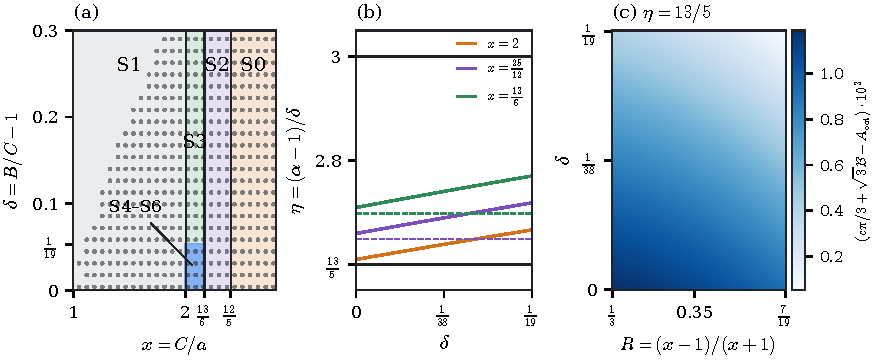
\includegraphics[width=\textwidth]{figures/fig-smaller-short.pdf}
 \caption{Parameter bounds from the gates. (a) The plane of the ratio $x=C/a$ and the displacement
 $\delta=B/C-1$. The dots are computed points of the equal-secant locus
 \eqref{eq:ss-equal-secants} with $1\le\alpha<x$. Gate S1 removes $x\le2$, S0 removes $x\ge12/5$,
 S2 removes $13/6\le x<12/5$ and S3 removes $\delta\ge1/19$, leaving the box where S4 to S6 work.
 (b) On that box, the slope $\eta=(\alpha-1)/\delta$ of the locus for $x=2,25/12,13/6$ (solid),
 between the lower order $1+4x(x+1)/(7x+1)$ (dashed) and the upper order $3$ of
 \cref{lem:ss-orders}. (c) The score gap
 $c\pi/3+\sqrt3\,\mathfrak B(u_*;R,T,\delta)-\Aoct$ of gate S6 at $\eta=13/5$:
 it is positive throughout the box.}\label{fig:smaller-short}
\end{figure}

\begin{proposition}[Gate S0]\label{prop:ss-S0}
Every smaller-short window has $x<12/5$, $D>0$ and $E_L>0$.
\end{proposition}

\begin{proof}[Proof sketch]
Suppose $x\ge12/5$. The root gives $R_\tau=0$ and $w\ge3/4$, so the floor-weighted residual
$G=R_\tau+\frac12(w-\frac34)$ is nonnegative at the actual window. Large ratios force an asymmetric
outer bridge: the equal secants and $x\ge12/5$ give $\alpha/\beta<3/4$ and then
$D<\alpha(\alpha+\beta)$. The weighted envelope \eqref{eq:ss-envelope} applies (its factor stays
positive for $x>5/3$), so $G^*_\tau\ge0$ at the actual scale, and the two shape facts make
$G^*_\tau$ increase with $u$. At fixed $p$ its value at the zero scale is negative, and an endpoint argument
for the quadratic in $q$ gives a nonnegative value at $q_{\max}$; the move along $\tau=2$ keeps it
nonnegative. On the face reached, $u$ is raised to the ceiling $\hat u(x,\beta)$ (central face) or
$\bar u(x,\beta)$ (outer face), and the duration is reduced to the three tests $F(2,\cdot)$,
$F(8\tau_{\max}/9,\cdot)$, $F(\tau_{\max},\cdot)$ of \cref{sec:ss-machinery}. The three face
signs of \cref{prop:ss-face-S0} say that each test is negative on the region cut out by the
orders. This
contradiction gives $x<12/5$. For $x\le12/5$ the identities
\begin{align*}
  D-\bigl[(1+2x)\alpha^2-2x^2\alpha+1+2x\bigr]&=2(\beta-\alpha x)(\alpha-x),\\
  (1+2x)\alpha^2-2x^2\alpha+1+2x-D_0&=(\alpha-1)\bigl[(1+2x)(\alpha+1)-2x^2\bigr],
\end{align*}
with $D_0=2+4x-2x^2\ge2/25$, give $D\ge\alpha D_0>0$. Finally
$E_L=\lambda(2\rho Du-E)>0$, because $E$ is at most its envelope value
$(1+x)(u-1)+\frac1{1+x}+\rho(2x+1)$, which is less than $2\rho Du$.
\end{proof}

\begin{proposition}[Gate S1]\label{prop:ss-S1}
Every smaller-short window has $x>2$.
\end{proposition}

\begin{proof}[Proof sketch]
Suppose $1<x\le2$. In this range we combine the residual with the upper bound $\Gamma<9193/50000$. Moving the opposite turn changes the Casimir $\Gamma(t,v)$ computed at
the central reverse run, but the combination $\Gamma-\frac{7}{96}R_\tau$ does not increase along
the two moves of \eqref{eq:ss-envelope}: in $v$ it is concave with a nonpositive slope at the
actual point, and along $v=\mathcal U(s)$ its derivative is the derivative of $R_\tau$, which is
negative, times a factor that stays below zero. Since $R_\tau=0$ at the actual window,
\[
  \Gamma\ge\Gamma_*-\tfrac{7}{96}R^*_\tau
\]
at the actual scale, where $\Gamma_*$ is the Gram expression at
$(t_0,\mathcal U(t_0))$. At fixed $p$ the right side decreases in $q$, and along $\tau=2$ the slope
of $R^*_2$ in $q$ exceeds one, so the right side does not increase when the point moves to a face.
On the central face $q=q_c\le1/7$ and on the outer face $q=1/7\le q_c$, the face signs
$\Gamma_*-\frac{7}{96}R^*_\tau>9193/50000$ for every admissible duration
(\cref{prop:ss-face-S1}) contradict $\Gamma<9193/50000$.
\end{proof}

\begin{proposition}[Gate S2]\label{prop:ss-S2}
A smaller-short window with $x<12/5$ has $x<13/6$.
\end{proposition}

\begin{proof}[Proof sketch]
Suppose $13/6\le x<12/5$. The weight is now variable, $m=2-7\tau/(4\tau_{\max})\in[1/4,2)$, and
the weighted residual $G_\tau=R_\tau+m(w-3/4)$ is still nonnegative at the root. The envelope
applies with this weight, the scale polynomial is convex in $q$ with a negative value at the zero
scale, and the $\tau=2$ continuation reaches the face $q^*=\min\{q_c,1/7\}$. After raising $u$ to
the ceiling $u_C(x,\beta)$ on the central face, and to $u_s(x,\beta)$ or $\bar V(x)$ on the outer
face, the face signs $G_\tau<0$ of \cref{prop:ss-face-S2} give the contradiction.
\end{proof}

\begin{proposition}[Gate S3]\label{prop:ss-S3}
A smaller-short window with $2\le x\le13/6$ has $\delta<1/19$.
\end{proposition}

\begin{proof}[Proof sketch]
Suppose $\delta\ge1/19$. The displacement is penalized by the weight
$m=4(4-3\tau/\tau_{\max})/(5\alpha-1)$, with which $G_\tau=R_\tau+m(w-3/4)\ge0$ at the root. On
this range $\beta<2\alpha$, so $D=\alpha^2+1+2x+2\beta(\alpha-x)>5\alpha^2-4\alpha x+1+2x\ge
6-2x>0$. The same three moves reach the face $q^*=\min\{q_c,1/7\}$. The duration is reduced to two
tests, $F_0$ at $\tau=2$ and $F_1$ at $\tau=\tau_{\max}$, the norm is raised to a ceiling, and on
the central face a monotonicity in $\beta$ moves the point to the curve
$\beta=x+\frac{25x}{15x+36}(\alpha-1)$. The face signs $F_0,F_1<0$ of
\cref{prop:ss-face-S3} give the contradiction.
\end{proof}

\subsubsection{Gate S4: the small box and a floor for the Casimir}\label{sec:ss-S4}

After gates S0 to S3 the shape lies in $2<x<13/6$, $0\le\delta<1/19$. Gate S6 needs a two-sided
control of $\alpha$ in terms of $\delta$, and also a lower bound for $\kappa$, because the
completion term in \eqref{eq:ss-defect} is weighted by $\kappa+3/2$.

\begin{proposition}[Gate S4]\label{prop:ss-S4}
A smaller-short window with $2\le x\le13/6$ and $\delta\le1/19$ has $\alpha\le1+3\delta$ and
$\Gamma>1829/10000$.
\end{proposition}

\begin{proof}[Proof sketch]
The first inequality is \cref{lem:ss-orders}(c), proved by the integral comparison in
\cref{app:ss-orders}. For the second, the monotonicity used in gate S1, now with the constant $1/7$,
gives $\Gamma\ge\Gamma_*-R^*_\tau/7$ at the actual scale. The scale
is moved at fixed $p$, and along $\tau=2$, up to the central scale $q_c$, and the duration maximum
\eqref{eq:ss-duration} leaves the two functions
\[
  \Phi=\Gamma_*(q_c)-\tfrac17R^*_2(q_c),\qquad
  \Psi=\Phi-\tfrac17(\tau_{\max}-2)\bigl(w_*(q_c)-\tfrac34\bigr).
\]
Both decrease in $u$, so the norm may be raised to its ceiling $\bar u(x,\beta)$
(\cref{app:ss-secant}). The face sign $\min\{\Phi,\Psi\}>1829/10000$ on the closed box
$2\le x\le13/6$, $0\le\delta\le1/19$, $\frac{13}{5}\delta\le\alpha-1\le3\delta$
(\cref{prop:ss-face-S4}) concludes.
\end{proof}

With \cref{lem:ss-orders} the window now lies in the \emph{small-shape domain}
\begin{equation}\label{eq:ss-small}
  2\le x\le\tfrac{13}{6},\qquad 0\le\delta\le\tfrac1{19},\qquad
  1+\tfrac{13}{5}\delta\le\alpha\le1+3\delta,
\end{equation}
that is $\alpha=1+\eta\delta$ with $13/5\le\eta\le3$ when $\delta>0$, and $\alpha=1$ when
$\delta=0$. No division by $\delta$ is used, so the symmetric boundary $\delta=0$ is included.

\subsubsection{Gate S5: the root forces a negative shear}\label{sec:ss-S5}

The defect inequality compares the cost of the bridge with the angle it turns, and both are
governed by one number. Let $M$ be the relative frame of the bridge, from the central switch to
the far switch. After a fixed rotation that depends only on $x$, its lower row does not depend on
$\rho$, and $\det M=1$ then determines the upper row up to one real parameter $h$, the
\emph{shear}. Put $R_x=(x-1)/(x+1)$, $T_s=(\beta-\alpha)/(\beta+\alpha)$,
$\mathcal U_1=\mathcal U(r)=(3+R_x^2)/4$, $\mathcal U_2=\mathcal U(r_A)=(3+T_s^2)/4$ and the
anisotropy $\nu=\mathcal U_1/\mathcal U_2-1\ge0$. Then
\begin{equation}\label{eq:ss-shear}
  \sqrt3\,h=\frac{(\beta x-\alpha)\bigl((x+2)\alpha+(2x+1)\beta\bigr)}
  {(1+x)^2(\alpha^2+\alpha\beta+\beta^2)}
  -2\,\mathcal U_1\,(2\beta x-x-\alpha\beta)\,\frac{\rho}{1-\rho}
.
\end{equation}
This is a strictly decreasing function of the central scale $\rho$, and the
bridge cost \eqref{eq:ss-cost} is affine in it:
\begin{equation}\label{eq:ss-cost-shear}
  \cost_{\mathrm{br}}=H_0-J_0h,\qquad J_0=\frac{3u}{2\,\mathcal U_1},\qquad
  H_0=\frac{\sqrt3}{2}\Bigl[\Bigl(1+\frac{u}{\mathcal U_1}\Bigr)R_x
   +\Bigl(1+\frac{u}{\mathcal U_2}\Bigr)T_s\Bigr].
\end{equation}
Decreasing the shear increases the bridge cost. Gate S5 shows that the actual outer root is
compatible only with a negative shear.

\begin{proposition}[Gate S5]\label{prop:ss-S5}
A smaller-short window in the small-shape domain \eqref{eq:ss-small} has
$q>\frac{15}{16}q_c$, $\sqrt3hR_x+\frac72\nu<0$, $h<0$ and $-hR_x>2\nu$.
\end{proposition}

\begin{proof}[Proof sketch]
Suppose $q\le q_b:=\frac{15}{16}q_c$. With weight zero, \eqref{eq:ss-envelope} and
\eqref{eq:ss-scale} give $\mathcal R(u;p,q):=\mathcal C(p)+q\mathcal L(p)\ge0$ at $p=\tau q$,
where $2q\le p\le r_A$. The residual is affine and increasing in $u$
(\cref{app:ss-S5}). The integral ceiling gives $u<19/25$ on the small-shape domain, so
$\mathcal R(19/25;p,q)\ge0$. At fixed $q$, however, the residual is concave in $p/r_A$ on its
allowed interval. Its tangent at $p=r_A$ has two endpoint values, both negative by the
shape comparisons in \cref{app:ss-S5}. This is a contradiction, so $q>q_b$.
The ratio comparison in \cref{app:ss-shear} then gives $-\sqrt3hR_x>7\nu/2$.
Since $R_x>0$ and $\nu\ge0$, this implies $h<0$ and $-hR_x>2\nu$, using $7>4\sqrt3$.
\end{proof}

\subsubsection{Gate S6: the completion cost bound}\label{sec:ss-S6}

\begin{proposition}[Gate S6]\label{prop:ss-S6}
For a smaller-short window in the small-shape domain with $\Gamma>1829/10000$, $h<0$ and
$-hR_x>2\nu$,
\[
  \cost_{\mathrm{br}}+\Bigl(\kappa+\frac32\Bigr)\Bigl(\frac\pi3-\theta_{\mathrm{br}}\Bigr)>\Aoct .
\]
\end{proposition}

The proof lowers the left side in four steps to an explicit function of the shape.

\runin{Step 1: lowering $\kappa$.} Since $12\cdot\frac{1829}{10000}-(\frac{40}{27})^2
=\frac{23}{1822500}>0$, the floor of gate S4 gives $\kappa>\kappa_0=40/27$. Since
$\theta_{\mathrm{br}}<\pi/3$, we may replace $\kappa+3/2$ by $c=\kappa_0+3/2=161/54$.

\runin{Step 2: the angle in terms of the shear.} Let $\psi=\arctan(R_x/\sqrt3)+\arctan(T_s/\sqrt3)$
be the angle of the fixed lower row of the rotated frame, let $K=\nu+2+2\kappa_0/J_0$, and
\[
  \delta(h)=2\arctan\frac{\sqrt{h^2+\nu^2}-h}{K+\sqrt{K^2-\nu^2}}.
\]
In the rotated basis, $\mathcal A+i\sqrt3\mathcal B$ is, up to a positive factor and the rotation
by $\psi$, a quadratic polynomial in one unknown entry of the costate at the central switch. The
condition that its values stay on one side of the line through the origin at angle $\psi+\delta$
is a discriminant inequality, which holds at $\delta=\delta(h)$. This gives
$\theta_{\mathrm{br}}\le\psi+\delta(h)$ for the actual shear. With
\eqref{eq:ss-cost-shear}, the left side of the proposition is at least
$H_0+c(\pi/3-\psi)+\tilde F(\delta(h))$, where $\tilde F(\delta)=-J_0\tilde h(\delta)-c\delta$ and
$\tilde h$ is the inverse of $h\mapsto\delta(h)$.

\runin{Step 3: continuation to the central scale.} The shear decreases in $\rho$, and $\rho<r^2$.
Let $h_c<h<0$ be the shear at the central scale $\rho=r^2$ and $\omega_c=\delta(h_c)$.
Throughout $[\delta(h),\omega_c]$, the quantity $H=-\tilde h$ satisfies
$\nu<HR_x/2$ and $H\le-h_c<R_x^2$. Together with the norm ceiling
$u\le3/4+R_x^2/12$, these bounds make $\tilde F$ strictly decreasing, by the
loss comparison in \cref{app:ss-S6}. The left side is therefore at least the central score
\[
  \mathcal F_c=\cost_c+c\Bigl(\frac\pi3-\psi-\omega_c\Bigr),\qquad
  \cost_c=\sqrt3\Bigl[\frac{u(2\beta x-x-\alpha\beta)}{x(x+2)}+\frac{R_x+T_s}{2}\Bigr] .
\]
Here $\cost_c$ is the bridge cost \eqref{eq:ss-cost} at the
central scale.

\runin{Step 4: minimizing the shape bound.} The integral estimate for the additional angle in
\cref{app:ss-S6} and a norm floor $u_*(R_x,\delta)$ obtained from the mean and variance of a
reciprocal integral give
\[
  \mathcal F_c>\frac{c\pi}{3}+\sqrt3\,\mathfrak B(u_*;R_x,T_s,\delta),
\]
with $\mathfrak B$ the function of \cref{app:ss-S6}, retaining the exact fixed-row angles. It is
concave in $T_s$, and $T_s$ is monotone in $\eta$, so its minimum over $13/5\le\eta\le3$ is
attained at an endpoint. The bound decreases with displacement, and at the largest displacement
it is concave in $R_x$. Its minimum is therefore at one of four corners
(\cref{prop:ss-face-S6}, \cref{fig:smaller-short}(c)), where a reciprocal-integral bound gives
$\mathfrak B>9/4000$. The direct octagon comparison of
\cref{lem:octagon-cost-comparison}, with $c/3=161/162$, now gives
\[
 \Aoct<\frac{c\pi}{3}+\frac{9\sqrt3}{4000}<\mathcal F_c.
\]


\subsubsection{Proof of \texorpdfstring{\cref{thm:m2-smaller-short}}{the theorem}}\label{sec:ss-assembly}

Let a smaller-short window be given. Gate S0 gives $x<12/5$, gate S1 gives $x>2$, and gate S2
then gives $x<13/6$. Gate S3 gives $\delta<1/19$, gate S4 gives $\alpha\le1+3\delta$ and
$\Gamma>1829/10000$, and \cref{lem:ss-orders} gives $\alpha\ge1+\frac{13}{5}\delta$. So the
window lies in the small-shape domain \eqref{eq:ss-small}. Gate S5 gives $h<0$ and
$-hR_x>2\nu$, and gate S6 then contradicts the window defect \eqref{eq:ss-defect}. \qed

\subsection{Estimates for the smaller-short window}\label{app:short-estimates}

This subsection gives the scalar inequalities behind \cref{sec:smaller-short}, organized by the
gate that uses them. They are identities between rational functions, and inequalities proved by
exhibiting a difference as a sum of terms of known sign, by the sign of a derivative on an
interval, or by monotonicity or convexity in one variable at a time. The face signs for gates
S0 to S4 in \cref{app:ss-faces} reduce, one variable at a time, to polynomials in one or two
variables, mostly of degree at most eight. We give the reductions and final signs; every
polynomial is specified by the rational expressions at the face where it is evaluated.
Gates S5 and S6 use the direct concavity and derivative comparisons given below.
Throughout, $\operatorname{Sec}$, $g_B$ and $\mathcal U$ are as in \cref{sec:ss-window}, and the
variables are those of \cref{tab:ss-variables}.

\subsubsection{Secants and the incoming norm}\label{app:ss-secant}

By \eqref{eq:ss-secant}, $(P_0-A_0)\operatorname{Sec}(A_0,B_0,P_0)$ is the integral of $g_{B_0}$
over $[A_0,P_0]$, hence additive over adjacent intervals, and by \eqref{eq:ss-g} every secant lies
in $[3/4,1]$. The function $g_{B_0}$ decreases on $(0,B_0]$ and increases on $[B_0,\infty)$. For
the bridge norm, \eqref{eq:ss-g} gives
\begin{equation}\label{eq:ss-u-integral}
  u-\frac34=\frac{1}{4(\beta-1)}\int_1^\beta\frac{(s-x)^2}{(s+x)^2}\,\dd s .
\end{equation}

\runin{The central value.} Normalize the integration variable by $x$ and put $a=1/x$.
Then
\[
 V(x)=\frac{1}{1-a}\int_a^1g(s)\,\dd s,\qquad g(s)=1-\frac{s}{(1+s)^2}.
\]
Since $g$ strictly decreases on $(0,1)$, adding $[0,a]$ strictly raises the average. Hence
$V$ increases with $x$ and
\[
 V(x)<V_\infty:=\int_0^1g(s)\,\dd s=\frac32-\log2,
 \qquad \lim_{x\to\infty}V(x)=V_\infty.
\]
With $z=(x-1)/(x+1)$ one also has $2x/(1+x)=1+z$ and
\[
  V(x)-\frac34=\operatorname{Sec}(1,x,x)-\frac34=\frac12+\frac z4-\frac{(1+z)\log(1+z)}{2z}.
\]
A lower bound for $\log(1+z)$ is therefore an upper bound for $V$.
The weighted Jensen bound $L_J(z)$ of \cref{lem:m2-logs}(c) gives
\[
 V(x)-\frac34<U(z):=\frac12+\frac z4-\frac{(1+z)L_J(z)}{2z}.
\]
This proves the ceiling used below,
\[
 V_G(x)=\frac34+\frac{(x-1)^2(71x^2+48x+1)}{96x(x+1)(13x^2+14x+3)},
\]
because direct subtraction gives the positive difference
\[
 V_G(x)-\frac34-U(z)=
 \frac{(x-1)^6}{96x(3x+1)(13x^2+14x+3)(21x^2+18x+1)}>0.
\]
Finally
\[
 \bar V(x)-V_G(x)=\frac{(x-1)^3(11x^2+96x+13)}{96x(x+1)(35x+13)(13x^2+14x+3)}\ge0
\]
gives $V\le\bar V=\frac34+\frac{2(x-1)^2}{(x+1)(35x+13)}$.

\runin{Ceilings and floors.} Splitting \eqref{eq:ss-u-integral} at $x$, bounding the integral over
$[1,x]$ by $(x-1)(\bar V-\frac34)$ or by a sharper rational bound, and bounding $(s-x)^2/(s+x)^2$
on $[x,\beta]$ by a quadratic or linear function of $s-x$, gives the rational ceilings of the
bridge norm used by the gates:
\begin{align*}
  \bar u&=\tfrac34+\tfrac{1}{\beta-1}\Bigl[\tfrac{2(x-1)^3}{(x+1)(35x+13)}
   +\tfrac{(\beta-x)^3}{48x^2}\Bigr],&
  \hat u&=\tfrac34+\tfrac{(x-1)^2(\beta+7x-8)}{4(x+1)(35x+13)(\beta-1)},\\
  u_\ell&=\tfrac34+\tfrac{(x-1)^2(\beta+15x-16)}{8(x+1)(35x+13)(\beta-1)},&
  u_C&=\tfrac34+\tfrac{680(x-1)^3+3(x+1)^2(\beta-x)}{9600(x+1)^2(\beta-1)},\\
  u_s&=\tfrac34+\tfrac{1}{\beta-1}\Bigl[\tfrac{17(x-1)^3}{240(x+1)^2}+\tfrac{\beta-x}{1200}\Bigr],&
  u_O&=\tfrac34+\tfrac{(x-1)^2(x+\beta-2)}{(\beta-1)(x+1)(35x+13)},\\
  u_{CB}&=\tfrac34+\tfrac{(x-1)(V_G(x)-3/4)+(\beta-x)/5808}{\beta-1},
\end{align*}
together with the floor $u_f=\frac34+\frac{(x-1)^2}{28(x+1)^2}$ and the integral floor $u_*$ of
gate S6 (\cref{app:ss-S6}). The ceiling $\bar u$ holds for all $1<x\le\beta$; each of the others
holds on the shapes where its gate uses it.

\subsubsection{Orders and the comparison argument}\label{app:ss-orders}

Normalize the shape by $\beta$: put $\ell=1/x$, $p_1=\alpha/\beta$, $q_1=x/\beta$ and
$\operatorname{avg}(p,q)=\operatorname{Sec}(p,1,q)$, the mean of $g(s)=1-s/(1+s)^2$ over $[p,q]$, with $\operatorname{avg}(p,p)=g(p)$ by continuity.
The equal secants \eqref{eq:ss-equal-secants} read
$\operatorname{avg}(\ell,1/q_1)=\operatorname{avg}(p_1,q_1)$. An order compares $p_1$ with a
\emph{barrier} $P(z)$, a differentiable function with $P(1)=\ell$, through the comparison function
\[
  \Phi(z)=\operatorname{avg}\bigl(P(z),z\bigr)-\operatorname{avg}(\ell,1/z),\qquad\Phi(1)=0 .
\]
Because $\operatorname{avg}$ decreases in its left end, the sign of $\Phi(q_1)$ decides whether
$p_1$ lies above or below $P(q_1)$.

\begin{lemma}[First contact]\label{lem:ss-first-contact}
Let $a<1$ and let $\Phi$ be continuous on $[a,1]$ with $\Phi(1)=0$. If $\Phi$ has a negative
derivative at each of its zeros in $(a,1]$, then $\Phi>0$ on $(a,1)$.
\end{lemma}

\begin{proof}
Since $\Phi(1)=0$ and $\Phi'(1)<0$, $\Phi>0$ on some interval $(1-\varepsilon,1)$. If
$\Phi(z_0)\le0$ for some $z_0\in(a,1)$, then $\Phi$ has a zero in $[z_0,1-\varepsilon]$; let $z^*$
be the largest one. Then $\Phi>0$ on $(z^*,1)$ and $\Phi(z^*)=0$, so $\Phi'(z^*)\ge0$, a
contradiction.
\end{proof}

At a zero of $\Phi$ both averages equal a common value $u$, and differentiation gives
\begin{multline*}
  \Phi'(z)\,(z-P(z))\,z\,(x-z)\\
  =-P'(z)\bigl(g(P(z))-u\bigr)z(x-z)-\bigl(u-g(z)\bigr)\bigl((2z-P(z))x-z^2\bigr).
\end{multline*}
Thus the sign at a contact depends on the ratio of the two endpoint gaps. We first bound this
ratio by comparing positive weights in its integral representation.

\begin{lemma}[Endpoint gaps]\label{lem:ss-endpoint-gaps}
For $0<p<q\le1$, put $m=\operatorname{avg}(p,q)$. Then
\[
 \frac{3-2p-q}{3-p-2q}
 +\frac{q-p}{6}<\frac{g(p)-m}{m-g(q)}
 <\frac{\log2-1/2}{3/4-\log2}.
\]
\end{lemma}

\begin{proof}
Write $d=q-p$ and
\[
 h(t)=-g'(p+dt)=\frac{1-p-dt}{(1+p+dt)^3},\qquad 0<t<1.
\]
Integration by parts gives
$g(p)-m=d\int_0^1(1-t)h(t)\,\dd t$ and
$m-g(q)=d\int_0^1th(t)\,\dd t$.
Their ratio is $(1-\mu)/\mu$, where $\mu$ is the mean of $t$ with weight $h$.
Multiplying a positive weight by a decreasing function lowers this mean: its covariance
with $t$ is the integral of $(t-s)(a(t)-a(s))/2$ against two copies of the probability measure,
and is nonpositive. Apply this to the linear weight $1-p-dt$ and the strictly decreasing
factor $(1+p+dt)^{-3}$. The ratio for the linear weight is
$(3(1-p)-d)/(3(1-p)-2d)$, giving the first term of the lower bound.

More generally, put $b=1-p$. The quotient $h(t)/[(b-dt)(1-\eta t)]$ decreases whenever
$0\le\eta\le3d/(1+p+4d)$: its logarithmic derivative has the sign of
$\eta(1+p+4dt)-3d$, which is negative for $0<t<1$. The same covariance comparison gives
\begin{equation}\label{eq:ss-gap-tilt}
 \frac{g(p)-m}{m-g(q)}>
 \mathcal Q_\eta(p,q):=
 \frac{\int_0^1(1-t)(b-dt)(1-\eta t)\,\dd t}
      {\int_0^1t(b-dt)(1-\eta t)\,\dd t}.
\end{equation}
These weights are positive on the interior, since $\eta<3/4$.
For the quantitative improvement take $\eta=d/2$, which is admissible because
$1+p+4d<6$. If $\mu_0$, $m_2$ and $\sigma^2$ are the mean, second moment and variance
for the linear weight, direct integration gives
\[
 \frac{\sigma^2}{\mu_0^2}
 =\frac13+\frac{d(6b-5d)}{6(3b-2d)^2}>\frac13,
\]
because $0<d\le b$. Tilting increases the gap ratio by
\[
 \frac{\eta\sigma^2}{\mu_0(\mu_0-\eta m_2)}
 >\frac{\eta\sigma^2}{\mu_0^2}>\frac\eta3=\frac d6.
\]
The denominator is positive, as it is a positive multiple of the first moment of the tilted
weight. This proves the stated refinement.

For the upper bound compare $h$ with $h_0(t)=(1-t)/(1+t)^3$. The quotient
\[
 \frac{h(t)}{h_0(t)}
 =\frac{1-p-dt}{1-t}\left(\frac{1+t}{1+p+dt}\right)^3
\]
increases: the two factors have derivatives with numerators $1-q\ge0$ and
$1+2p-q>0$, respectively. Thus $h$ has a larger mean than $h_0$ and a smaller gap ratio.
The latter ratio is exactly $(\log2-1/2)/(3/4-\log2)$. Its numerator and denominator are
positive integrals of $(1-t)h_0(t)$ and $th_0(t)$, respectively, so no numerical logarithm
bound is needed.
\end{proof}

\runin{The global upper order.} Take $k=5/4$ and $P(z)=\ell+k(1-z)$. If $P(q_1)\ge q_1$, the
upper bound $p_1\le P(q_1)$ is automatic from $p_1<q_1$. On the interval $P(z)<z$, put
\[
 a=1-\ell,\qquad \theta=\frac{1-z}{a},\qquad
 R_0=\frac{3-2P(z)-z}{3-P(z)-2z}.
\]
Here $0<a<1$ and $0\le\theta<4/9$, since $P(z)<z$.
The following identity makes the contact sign positive:
\begin{align*}
 &kR_0z(x-z)-\bigl((2z-P(z))x-z^2\bigr)\\
 &\quad=\frac{a}{4(1-a)(4+3\theta)}\Bigl[
 1+6\theta^2+7(3\theta-1)^2\\
 &\qquad\qquad
 +6(1-a)\theta\bigl(2(4-9\theta)+7\theta^2\bigr)
 +6(1-a)^2\theta^2(4-7\theta)\Bigr]>0.
\end{align*}
Every factor in the bracket is nonnegative, and the constant term is positive.
By the lower gap bound of \cref{lem:ss-endpoint-gaps}, $\Phi'>0$ at every zero,
including $z=1$. Apply \cref{lem:ss-first-contact} to $-\Phi$: then $\Phi<0$ to the left of
one, and decreasing the left endpoint of the average gives $p_1<P(q_1)$ if $q_1<1$.
This proves the upper order $\alpha\le\beta/x+\frac54(\beta-x)$ of \cref{lem:ss-orders}(b).
If $q_1=1$, equality of the two averages forces $p_1=\ell$, so the same bound holds.

\runin{The upper order for $x\le5$.} Now take $k=9/8$ and $P(z)=\ell+k(1-z)$.
Again only the interval $P(z)<z\le1$ needs a comparison. Put
\[
 a=1-\ell,\qquad 0\le\theta=\frac{1-z}{a}<\frac8{17},\qquad
 E=1+\frac78\theta,\qquad D=1-\frac{17}{8}\theta>0.
\]
Let $R_0=(3-2P(z)-z)/(3-P(z)-2z)$ and define the normalized contact expression
\[
 \mathcal N(\ell,\theta)=\frac{E(1-a)}a
 \left[kR_0z(x-z)-\bigl((2z-P(z))x-z^2\bigr)\right].
\]
This expression does not decrease in $\ell$. Indeed,
\[
 \partial_\ell\mathcal N
 =\frac\theta{32}\left[73\theta^2-186\theta+80
                   +2\ell\theta(40-73\theta)\right]\ge0.
\]
On $0\le\theta<1/2$, the first quadratic decreases and is at least its value $21/4$ at
$1/2$; also $40-73\theta>7/2$.
By the refined gap bound, the actual normalized contact sign is strictly greater than
\[
 \mathcal N+\frac3{16}aDE(1-a\theta)(1+\ell\theta)
 \ge\mathcal N+\frac3{16}aD(1-\theta).
\]
For $1<x\le3$, use $\ell\ge1/3$ and the identity
\[
 \mathcal N(1/3,\theta)
 =\frac94\left(\theta-\frac13\right)^2
       +\frac{\theta(30+53\theta+292\theta^2)}{576}>0.
\]
For $3\le x\le5$, use $a\ge2/3$ and $\ell\ge1/5$. The lower bound is then at least
\begin{align*}
 \mathcal N(1/5,\theta)+\frac18D(1-\theta)
 &=\frac{27}{8}\left(\theta-\frac13\right)^2
    +\theta\left(\frac5{64}-\frac{13\theta}{160}\right)
    +\frac{73\theta^3}{200}\\
 &\ge\frac{27}{8}\left(\theta-\frac13\right)^2+\frac{3\theta}{80}>0,
\end{align*}
since $\theta<1/2$. The contact derivative is therefore positive in both ranges.
The same first-contact argument as for $k=5/4$ gives
$\alpha\le\beta/x+\frac98(\beta-x)$, including equality when $\beta=x$.

\runin{The upper order in the small box.} We prove \cref{lem:ss-orders}(c).
Here $q_1=1/(1+\delta)\ge19/20$, so it suffices to compare barriers on $19/20\le z\le1$.
If $x\le16/9$, the upper order just proved gives
$\alpha\le1+(1+9x/8)\delta\le1+3\delta$.

For $16/9\le x\le2$, take $P(z)=\ell+1-z$, put $a=1-\ell$ and $\theta=(1-z)/a$,
and use \eqref{eq:ss-gap-tilt} with $\eta=(z-P(z))/2$.
We have $a\ge7/16$ and $\theta\le4/35<1/8$. Direct integration of the tilted linear weight gives
\begin{align*}
 &\mathcal Q_\eta(P(z),z)z(x-z)-\bigl((2z-P(z))x-z^2\bigr)\\
 &\quad=\frac{a^2(1-2\theta)}{(1-a)(4a\theta^2+4\theta-a+4)}
 \bigl[1-6\theta-6\theta^2-2a(1-a)\theta^3\bigr]>0.
\end{align*}
The bracket exceeds $1-6/8-6/64-1/1024>0$, using $a(1-a)\le1/4$.
First contact therefore gives $\alpha\le\beta/x+(\beta-x)=1+(1+x)\delta\le1+3\delta$.

It remains to consider $2\le x\le13/6$, so $6/13\le\ell\le1/2$.
Take $P(z)=\ell(3-2z)$ and, at a contact, put
$p=P(z)$, $s=1-z$, $b=1-p$ and $d=z-p=b-s$.
The maximal tilt $\eta=3d/(1+p+4d)$ in \eqref{eq:ss-gap-tilt} has the ratio
\[
 \mathcal T(b,s):=\mathcal Q_\eta(p,z)=\frac ND,\qquad
 \begin{aligned}
 N&=9b^2-10bs-5s^2+8b+4s,\\
 D&=3b^2-2bs-7s^2+4b+8s.
 \end{aligned}
\]
We compare $2\ell\mathcal T$ with
$M=1+(z-p)/[z(1-\ell z)]$, since their difference has the sign of the contact derivative.
On this rectangle $9/20\le b\le7/13$, $0\le s\le1/20$ and $p\le11/20$.
Also $d/b\ge8/9$, so the linear-weight ratio is at least $19/11$ and
$\mathcal T>17/10$. The positive expressions above give
\[
 D>\frac{12}{5},\qquad N_b<18,\qquad D_b>\frac{13}{2},\qquad
 \mathcal T_b=\frac{N_b-\mathcal T D_b}{D}<3.
\]
For the first inequality use $D\ge b(3b+4)$; for the last use
$18-(17/10)(13/2)<3(12/5)$. Consequently
\[
 \partial_p(p\mathcal T)=\mathcal T-p\mathcal T_b>\frac1{20},\qquad
 M_\ell=\frac{(z-1)(z+3)}{z(1-\ell z)^2}\le0.
\]
Thus $2\ell\mathcal T-M$ increases in $\ell$, and it suffices to take $\ell=6/13$.

Along this edge $b=(7-12s)/13$. Write $k=12/13$ for $b_z$.
The two quadratics satisfy
$N_{zz}=18k^2+20k-10>0$ and $D_{zz}=6k^2+4k-14<0$.
Their endpoint values and the upper tangent to $D$ at $z=1$ give
\[
 N_z\ge N_z(19/20)>16,\qquad
 D_z\le D_z(19/20)<\frac18,\qquad D<\frac{31}{10}.
\]
Moreover $\mathcal T<5/2$, since
$5D-2N=b(4-3b)+s(10b+32-25s)>0$.
It follows that
\[
 \mathcal T_z=\frac{N_z-\mathcal T D_z}{D}
 >\frac{16-5/16}{31/10}>5.
\]
On the same edge,
\[
 M_z=\frac{6(25z^2-36z+39)}{z^2(13-6z)^2}<4:
\]
its numerator is at most $168$, while $z(13-6z)>13/2$.
Therefore $(2\ell\mathcal T-M)_z>8/13>0$, and the smallest value is at $z=19/20$.
At that corner $s=1/20$ and $d=23/52$. The inequality
$(23/52)^2>39/200$ gives $N-2D=3d^2-6s(2-s)>0$, so $\mathcal T>2$.
Also $d<4/9$ and $z(1-\ell z)>8/15$, giving $M<11/6<24/13=4\ell$.
The contact sign is positive. First contact gives $p_1\le\ell(3-2q_1)$, or
$\alpha\le3\beta/x-2=1+3\delta$, as required.

\runin{Feasibility of a lower barrier.} The lower-order proofs below use the following observation.
Suppose $0<z_m<1$, $P(1)=\ell$, $P(z_m)=z_m$ and $P(z)<z$ for $z_m<z\le1$.
If its comparison function $\Phi$ is positive on $(z_m,1)$, the actual equal-secant shape
must have $q_1>z_m$. Indeed, put
\[
 H(b)=\int_\ell^b g(s)\,\dd s-(b-\ell)g(b),\qquad b\ge1.
\]
This decreases because $H'(b)=-(b-\ell)g'(b)\le0$.
At the actual shape, $\operatorname{avg}(\ell,1/q_1)=\operatorname{avg}(p_1,q_1)>g(q_1)$,
so $H(1/q_1)>0$, using $g(1/q_1)=g(q_1)$.
It follows that $\operatorname{avg}(\ell,1/z)>g(z)$ for $q_1\le z\le1$.
If $q_1\le z_m$, this makes $\Phi(z_m)<0$, contrary to continuity and
$\Phi>0$ on $(z_m,1)$. Thus $q_1>z_m$.

\runin{The strong lower order.} We prove \cref{lem:ss-orders}(a), without a restriction on $x$.
Put $a=1-\ell\in(0,1)$ and $k=4(2-a)/(8-a)\in(0,1)$, and take $P(z)=\ell+k(1-z)$.
For $p=P(z)<z$, use the relative endpoint deficits
\[
 b=1-p,\qquad r=\frac{1-z}{1-p},\qquad
 b=\frac{a}{1+kr},\qquad 0<b<1,\quad 0\le r<1.
\]
Write $\mathcal R(b,r)$ for the endpoint-gap ratio on $[1-b,1-br]$.
At fixed $r$ its integral weight, up to a constant factor, is
\[
 w_b(t)=\frac{v(t)}{(2-bv(t))^3},\qquad v(t)=1-(1-r)t.
\]
The ratio $w_{b_2}/w_{b_1}$ decreases in $t$ when $b_2>b_1$: its logarithmic derivative
with respect to $v$ is $6(b_2-b_1)/[(2-b_1v)(2-b_2v)]>0$.
The covariance argument in \cref{lem:ss-endpoint-gaps} therefore shows that $\mathcal R$
increases in $b$.

Simpson's bound for the reciprocal integral gives a convenient upper estimate. In the form
\[
 L(y)=\frac{y-1}{6}\left(1+\frac8{1+y}+\frac1y\right),\qquad
 (L-\log)'(y)=\frac{(y-1)^4}{6y^2(1+y)^2},
\]
it follows directly that $\log y<L(y)$ for $y>1$.
Substitute $y=(1+q)/(1+p)$ in
\[
 \operatorname{avg}(p,q)=1+\frac1{(1+p)(1+q)}
                         -\frac{\log y}{q-p}.
\]
The resulting lower mean $m_L$ lies above $g(q)$: for $p=1-b$, $q=1-br$,
\[
 m_L-g(q)=\frac{b^2(1-r)\,[4+8r-br(5+r)]}
 {6(2-b)(2-br)^2(4-b-br)}>0,
\]
since the bracket is at least $4+3r-r^2>0$.
The gap ratio decreases as the mean increases, so
\[
 \mathcal R(b,r)<\widehat{\mathcal R}(b,r):=
 \frac{2-br}{2-b}\,
 \frac{8+4r-b(1+5r)}{4+8r-br(5+r)}.
\]

The slope satisfies
$k-(1-a/2)=a(2-a)/[2(8-a)]>0$.
Thus $b\le b_*:=a/[1+(1-a/2)r]$, and comparison of the weights followed by the last bound gives
$\mathcal R(b,r)<\widehat{\mathcal R}(b_*,r)$.
Set $B=1+(1-r)(2/k-1)/[1+(2-a)r]$ and write
\begin{align*}
 H_*&=4+(12-7a)r+(8-5a)r^2,\\
 Q&=(1+r)\{4(1-a)(7r+1)+a(9r+11)\}+2a(1-a)r(5-r).
\end{align*}
Multiplication of the two fractions gives the positive-product identity
\[
 B-\widehat{\mathcal R}(b_*,r)
 =\frac{ar(1-r)Q}{2(2-a)(1+r)(1+(2-a)r)H_*}\ge0.
\]
Here $H_*,Q>0$, so $\mathcal R<B$, also when $r=0$ by the strict Simpson bound.

It remains to compare this upper bound with the contact threshold
$M=1+(z-p)/[z(1-\ell z)]$.
Put $h=k-a$ and
\[
 B_0=1+\frac{(1-r)(2/k-1)}{1+(1+h)r}.
\]
Since $k<1$, we have $B\le B_0$, while substitution of
$p=1-a/(1+kr)$ and $z=1-ar/(1+kr)$ gives
\[
 M-kB_0=
 \frac{r\bigl[(1-r)(2-k(1+h))+r(1-k)(1+h)(2+h)\bigr]}
 {(1+hr)(1+(1+h)r)}\ge0.
\]
Here $-1<h<k<1$ and $2-k(1+h)>2-k(1+k)=(1-k)(k+2)>0$.
Consequently $k\mathcal R<kB\le kB_0\le M$, so $\Phi'<0$ at every zero, including $z=1$.
First contact gives $\Phi>0$ between the crossing $P(z_m)=z_m$ and $1$.
The preceding feasibility argument, applied to this crossing,
shows that the actual $q_1>z_m$.
Thus $p_1>P(q_1)$ when $q_1<1$; when $q_1=1$, $p_1=\ell$.
Multiplying by $\beta$ proves the claimed lower order.

\runin{The quadratic lower order.} For \cref{lem:ss-orders}(d), retain $a=1-\ell$ and
$k=4(1+\ell)/(7+\ell)$, but curve the barrier:
\[
 P(z)=\ell+ks+\frac{\ell s^2}{1+3s},\qquad s=1-z.
\]
Here $6/13\le\ell\le1/2$, so
\[
 \frac12\le a\le\frac7{13},\qquad
 \frac34<k\le\frac45,\qquad \frac15<k-a\le\frac3{10}.
\]
For $p=P(z)<z$, put
\[
 K=k+\frac{\ell s}{1+3s},\qquad
 j=-P'(z)=K+\frac{\ell s}{(1+3s)^2},\qquad
 r=\frac{s}{1-p}.
\]
Then $0\le r<1$, $b=1-p=a/(1+Kr)$ and $s=ar/(1+Kr)$.
The condition $p<z$ gives $s<a/(1+k)<1/3$, hence $k\le K<9/10$ and $j\ge k>3/4$.
At a contact it suffices to prove $j\mathcal R(b,r)<M(K)$, where
\[
 M(v)=1+\frac{(1-r)(1+vr)}{(1+(v-a)r)(1+(v+\ell)r)}.
\]
This is the contact threshold $1+(z-p)/[z(1-\ell z)]$ when $v=K$.

First keep the positive gain in the preceding comparison. With the same $B,B_0,H_*,Q$ as
there, put $E=B-\widehat{\mathcal R}(b_*,r)\ge0$.
Since $K\ge k$, comparison of the weights still gives
$\mathcal R(b,r)<B-E$.
Write $D=M(k)-kB_0$. The preceding positive-product identity and the bounds on $k-a$ give
\[
 D\ge\frac{r\bigl[\frac{19}{20}(1-r)+\frac12r\bigr]}
 {(1+3r/10)(1+13r/10)}.
\]
Indeed its two numerator factors $2-k(1+k-a)$ and
$(1-k)(1+k-a)(2+k-a)$ exceed $19/20$ and $1/2$.
The remaining two gains satisfy
\begin{equation}\label{eq:ss-quadratic-gains}
 k(B_0-B)\ge\frac{r(1-r)}{5(1+2r)^2},\qquad
 jE\ge\frac{r(1-r)}{5(1+2r)^2}.
\end{equation}
For the first, subtract the two fractions:
\[
 k(B_0-B)=\frac{r(1-r)(2-k)(1-k)}
 {(1+(1+k-a)r)(1+(2-a)r)}.
\]
Both denominator factors are at most $1+2r$ and $(2-k)(1-k)>1/5$.
For the second, the positive expressions for $Q,H_*$ give
\[
 Q\ge7(1+r)(1+3r/2),\qquad H_*\le4(1+2r)^2.
\]
Together with $a/[2(2-a)]\ge1/6$ and $2-a\le3/2$, these imply
$E\ge7r(1-r)/[24(1+2r)^2]$. Now use $j>3/4$ and $7/32>1/5$.

Next bound the two costs of curving the barrier. Set $\eta=K-k$. The identities for $s$ give
\[
 \eta=\frac{\ell ar}{1+(K+3a)r},\qquad
 j-k=\frac{\ell ar\,[2+(2K+3a)r]}{(1+(K+3a)r)^2}.
\]
Since $\ell a\le1/4$, $K+3a>9/4$ and $2K+3a<7/2$,
\begin{equation}\label{eq:ss-quadratic-costs}
 \eta\le\frac{r}{4(1+9r/4)},\qquad
 j-k\le\frac{r(2+7r/2)}{4(1+9r/4)^2}.
\end{equation}
Also $2/k-1<8/5$ and $2-a>7/5$, so $B\le(13-r)/(5+7r)$.
For the change in $M$, put
\[
 F(v)=\frac{1+vr}{(1+(v-a)r)(1+(v+\ell)r)},\qquad k\le v\le K.
\]
With $u=1+(v-a)r\ge1+r/5$, direct differentiation gives
\[
 0\le-F'(v)=\frac{r(u^2+2aru+ar^2)}{u^2(u+r)^2}\le\frac r u.
\]
For the last inequality compare the three numerator terms with those of $u(u+r)^2$,
using $u\ge1>a$. Integration over $[k,K]$, followed by \eqref{eq:ss-quadratic-costs}, yields
\[
 0\le M(k)-M(K)\le\frac{(1-r)\eta r}{1+r/5}
 \le\frac{r^2(1-r)}{4(1+9r/4)(1+r/5)}.
\]

For $r>0$, normalize by $S=(1+2r)^2/r$.
The three denominator comparisons
\begin{gather*}
 (1+3r/10)(1+13r/10)\le1+2r,\\
 1+2r\le1+9r/4,\\
 (1+9r/5)(1+r/5)\ge1+2r
\end{gather*}
give
\begin{align*}
 SD&\ge\left(\frac{19}{20}-\frac9{20}r\right)(1+2r),\\
 S(j-k)B&\le\frac{(4+7r)(13-r)}{8(5+7r)}
       \le\frac{13}{10}+\frac r{10}+\frac3{10}r(1-r),\\
 S\bigl(M(k)-M(K)\bigr)&\le\frac{r(1-r)(1+9r/5)}4.
\end{align*}
The second upper bound follows by division:
\[
 \frac{(4+7r)(13-r)}{8(5+7r)}
 =\frac{13}{10}+\frac{3r}{40}+\frac{7r(1-r)}{5(5+7r)}.
\]
Combining these estimates with \eqref{eq:ss-quadratic-gains} gives
\begin{align*}
 S\bigl(M(K)-j\mathcal R(b,r)\bigr)
 &>\left(\frac{19}{20}-\frac9{20}r\right)(1+2r)+\frac25(1-r)\\
 &\quad-\left(\frac{13}{10}+\frac r{10}+\frac3{10}r(1-r)\right)
       -\frac{r(1-r)(1+9r/5)}4\\
 &=\frac{1+r^3}{20}+\frac25r(1-r)^2>0.
\end{align*}
When $r=0$, $j=k$, $M(K)=2$ and $E=0$, while the Simpson bound still gives
$\mathcal R<B=2/k$. Thus the contact derivative is negative in this case as well.

The function $P(z)-z$ decreases strictly and has a unique zero $z_m\in(0,1)$.
First contact gives $\Phi>0$ on $(z_m,1)$; the same feasibility function $H$ as above excludes
$q_1\le z_m$. Hence $p_1>P(q_1)$ for $q_1<1$, with equality for $q_1=1$.
Finally, $s=\delta/(1+\delta)$ and multiplication by $\beta=x(1+\delta)$ transform the barrier into
\[
 \beta P(q_1)=1+(1+xk)\delta+\frac{\delta^2}{1+4\delta},
\]
which is the order claimed in part (d).

\subsubsection{The outer scale bound}\label{app:ss-scale}

\begin{lemma}[Reverse-centre scale bound]\label{lem:ss-outer-scale}
At a reverse centre with neighbour ratios $0<r,t<1/2$, scale $0<\rho<rt$, and norms
$3/4\le u\le\mathcal U(r)$, $3/4\le v\le\mathcal U(t)$ and the stationarity
$E=1+r+t-\rho+\log\frac{\rho}{rt}-\frac{1-u}{r}-\frac{1-v}{t}$, the inequality
$(4uv-E^2)/(16(1-\rho)^2)<9193/50000$ implies $\rho<1/7$.
\end{lemma}

\begin{proof}
Assume $\rho\ge1/7$. First consider the pairing $E_0$ at $u=v=3/4$.
With $\sigma=rt$ and $\chi=r+t$, the inequalities $r,t<1/2$ give
$\chi\le1/2+2\sigma$, so
\[
 E_0=1-\rho+\log\frac\rho\sigma+\chi\left(1-\frac1{4\sigma}\right)
 \ge L(\sigma):=1-\rho+\log\frac\rho\sigma+2\sigma-\frac1{8\sigma}.
\]
Since $L'(\sigma)=(4\sigma-1)^2/(8\sigma^2)\ge0$ and $\sigma>\rho$,
$E_0\ge L(\rho)=1+\rho-1/(8\rho)>0$. The pairing increases with either norm, hence $E\ge E_0>0$.

The switch ceilings also give $E<-1+2r+2t-rt\le3r/2$, and symmetrically $E\le3t/2$.
For the first inequality use that $\log\rho-\rho$ increases for $\rho<1$; for the second use
$-1+r/2+2t-rt=(1-2t)(r/2-1)\le0$. Consequently
\[
 \partial_u(4uv-E^2)=4v-\frac{2E}{r}\ge4v-3\ge0,
\]
and the analogous derivative in $v$ is nonnegative. Lowering both norms to $3/4$ therefore
lowers the Gram quotient. At those norms,
$\partial_rE_0=(r-1/2)^2/r^2\ge0$, and likewise for $t$.
Letting both ratios increase to $1/2$ raises the positive pairing and lowers the quotient again:
\[
 \frac{4uv-E^2}{16(1-\rho)^2}\ge
 G(\rho):=\frac{9/4-B(\rho)^2}{16(1-\rho)^2},\qquad
 B(\rho)=1-\rho+\log4\rho .
\]
On $[1/7,1/4)$ the function $B$ is positive, and $G$ increases by the fixed-$S$
monotonicity in the proof of \cref{lem:m1-symmetric}, at $S=0$.
To estimate the initial value, pair the reciprocal integral about its midpoint.
With $m=11/8$ and $h=3/8$, strict Jensen gives
\[
 \log\frac74=2m\int_0^h\frac{\dd t}{m^2-t^2}
 >\frac{2mh}{m^2-h^2/3}=\frac{33}{59}.
\]
Here Jensen applies to the strictly convex function $s\mapsto1/s$ and the nonconstant
positive function $m^2-t^2$, whose average is $m^2-h^2/3$.
Since $0<B(1/7)<6/7-33/59$,
\[
 G(1/7)>\frac{9/4-(6/7-33/59)^2}{16(6/7)^2}>\frac{9193}{50000},
\]
where the last step is an exact rational comparison. This contradicts the assumed Casimir cap.
\end{proof}

Applied at the outer centre $A$, with $r=r_A$, $t=1/\tau$, $\rho=q$, norms $u,w$ and pairing
$E_L$, the lemma gives $q<1/7$ (\cref{lem:ss-first}(e)).

\subsubsection{The comparison transformations}\label{app:ss-moves}

The transformations in \cref{sec:ss-machinery} use the following formulas.

\runin{The scale coefficients.} With $\varepsilon=1-\alpha^{-2}$, $n=(1+x)/\alpha^2$,
$g=D/\alpha^2$ and $E_0=(1+x)(u-1)+1/(1+x)$, the coefficients of \eqref{eq:ss-scale} are
\begin{align*}
  A_1&=2\varepsilon+n+gE_0,\\
  A_2&=\varepsilon^2+\varepsilon n+n^2+g^2u+g\varepsilon E_0-g\bigl(2(1+x)-1\bigr)/\alpha^2,\\
  A_3&=2gu+\varepsilon E_0-\bigl(2(1+x)-1\bigr)/\alpha^2.
\end{align*}
The two scales are related by $\rho/(1-\rho)=q/(\alpha^2(1-q))$, and $q=q_c$ exactly when
$\rho=r^2$; also $q_c\le1/7$ if and only if $6\alpha^2\le x(x+2)$.

\runin{The duration tests.} The identity \eqref{eq:ss-duration} is the logarithm bound
$\log y\le(y-1/y)/2$ at $y=\tau/2$. For the three tests of gate S0, the logarithm
$\log(\tau/\tau_{\max})$ is bounded by $\log y\le y-1$ and by the tangent
$\log y\le\frac54y-\frac{11}{9}$ at $y=4/5$ (using $\log\frac54\ge\frac29$), and $1/\tau$ by its
chord; an affine function of $\tau$ is then at most its larger endpoint value. This gives the
values $\tau=2$, $8\tau_{\max}/9$ and $\tau_{\max}$, with the logarithm replaced by
$\frac{5}{2\tau_{\max}}-\frac{11}9$, $-\frac19$ and $0$ respectively.

\subsubsection{Gates S0 to S4}\label{app:ss-S0-S4}

Apart from the face signs of \cref{app:ss-faces}, these gates use the following inequalities.

\runin{Gate S0.} The positive diagonal is in the proof of \cref{prop:ss-S0}. For the positive
pairing, the envelope bound for $E$ and the replacements $D\ge D_0$ and
$u\le u_0=\frac34+\frac{(x-1)^2}{12(x+1)^2}$ give
$E-2\rho Du\le\Lambda(\rho):=\bigl((1+x)-2\rho D_0\bigr)u_0-(1+x)+\frac1{1+x}+\rho(2x+1)$, affine
in $\rho\in[0,(1+x)^{-2}]$, with
\begin{align*}
  \Lambda(0)&=-\frac{(x-1)(x+5)}{6(1+x)},\\
  \Lambda\bigl((1+x)^{-2}\bigr)&=-\frac{x^5-13x^4+6x^3+32x^2+37x+9}{6(1+x)^4},
\end{align*}
both negative on $1<x\le12/5$. The shape bound $\alpha/\beta<3/4$ for $x\ge12/5$ compares two
bounds for $u-3/4$: if $\alpha\ge3\beta/4$ then
$u-\frac34\le\frac{(\beta-\alpha)^2}{4(\beta+\alpha)^2}\le\frac1{196}$, while
\eqref{eq:ss-u-integral} and the tangent bound $1/y^2\ge1/c^2-2(y-c)/c^3$ give
$u-\frac34\ge\frac{4(x-1)^3}{(4x-3)(5x+3)^2}$, which increases in $x$ and exceeds $1/196$ at
$x=12/5$.

\runin{Gate S1.} The combination $\Gamma-\frac{7}{96}R_\tau$ is monotone along the envelope path
because the ratio of the derivatives of $\Gamma$ and $R_\tau$ along that path is at most $7/96$.
Along $\tau=2$ the slope of $R^*_2$ in $q$ exceeds one: after completing the square in $\Delta q$
with $\Delta=D/\alpha^2$, $q\,\dd R^*_2/\dd q$ is bounded below by a quadratic in
$a=\alpha^{-2}\in(0,1]$ with nonpositive leading coefficient, and its values at $a=0$ and $a=1$
exceed $1/7\ge q$ by explicit rational functions of $z=x-1$ whose numerators have positive
coefficients.

\runin{Gate S4.} At the central scale put
\[
 S=1+x,\quad V=x(x+2),\quad N=\alpha^2+V,\quad
 R=\frac{x-1}{x+1},\quad d=\frac DN,\quad C_*=\frac{S^3}{N}.
\]
Here $q_c=\alpha^2/N$, $\rho(q_c)=S^{-2}$ and $\Gamma_c:=\Gamma_*(q_c)$.
The central row and Gram determinant have the compact form
\[
 16\Gamma_c=3-b_0^2-2Rb_0,\qquad
 b_0=\frac{S^3(\mathcal U_1-u)}V,\quad
 \mathcal U_1=\frac{3+R^2}{4}.
\]
Consequently $\partial_u\Gamma_c=S^3(b_0+R)/(8V)$.
For $u\ge3/4$, $S^3/V=S(1+1/V)<18/5$ and $R^2<1/7$ give
$b_0<9/70<1/6$. Since $R<3/8$,
\[
 \partial_u\Gamma_c<\frac{18}{5}\frac{1/6+3/8}{8}<\frac14.
\]

The transport formulas give
\[
 \partial_uw_*=d^2-dC_*,\qquad
 \partial_uE_{L,*}=2d-C_*,
\]
so the exact residual at any duration satisfies
\[
 \partial_uR^*_\tau
 =\frac1{r_A}+C_*(1-\tau d)+\tau d^2-2d>2.
\]
To see the last sign, first note that $0<D<S$.
On this box $\alpha\ge1$, $\beta\le130/57$ and $x-\alpha\le7/6$, so
$D=\alpha^2+1+2x-2\beta(x-\alpha)\ge116/171>0$.
For the upper bound use $\beta\ge x$ and
$\alpha\le22/19$:
$D-S\le\alpha^2+2\alpha x+x-2x^2\le\alpha^2+4\alpha-6<0$;
the middle expression decreases in $x\ge2$, and $(22/19+2)^2<10$.
As $N\ge S^2$, it follows that $d<1/S\le1/3$.
Also $r_A\le11/30<3/8$ and
$\tau d\le\tau_{\max}d=gr_A<1$; the last inequality is
$\beta(2x-\alpha)>1+2x$, proved directly in \cref{app:ss-S5}.
Thus the positive $C_*$ term may be discarded and
$\partial_uR^*_\tau>1/r_A-2d>2$.

It follows that $\partial_u(\Gamma_c-R^*_\tau/7)<0$ for every
$2\le\tau\le\tau_{\max}$ and every $u\ge3/4$.
For $\Phi$ this is the duration $2$. For $\Psi$ it is the duration $\tau_{\max}$:
the difference between its affine duration bound and $R^*_{\tau_{\max}}$ is independent of $u$,
by \eqref{eq:ss-duration}. Hence both S4 tests decrease in the norm throughout this range.

\subsubsection{Gate S5}\label{app:ss-S5}

\runin{Monotonicity in the norm.} At fixed shape, scale and duration the residual
$\mathcal R(u;p,q)$ is affine in $u$, with
\[
  \partial_u\mathcal R=(1+x)+\frac1{r_A}-pg(1+x)+q\bigl\{p\bigl(g^2+g\varepsilon(1+x)\bigr)-2g
  -\varepsilon(1+x)\bigr\}.
\]
It is positive throughout the small-shape domain, for $0\le q<1/2$ and $0<p\le r_A$.
Indeed, $\alpha\le22/19<3/2$ and $\beta\ge x\ge2$ imply
\[
 \beta(2x-\alpha)>x(2x-3/2)\ge1+2x,
\]
where the second difference is $(x-2)(2x+1/2)\ge0$. Since
$D=\alpha(\alpha+\beta)+1+2x-\beta(2x-\alpha)$, this gives $gr_A<1$.
Now factor the derivative as
\[
 \partial_u\mathcal R=(1+x)(1-\varepsilon q)(1-pg)
             +\frac1{r_A}-qg(2-pg).
\]
If $g\le0$, positivity is immediate. If $g>0$, then $0<pg\le r_Ag<1$,
so the first term is positive and the remaining terms are at least
$(1-2q)/r_A>0$. Here $0\le\varepsilon<1$ because $\alpha\ge1$.

\runin{The ceiling.} The integral defining $V(x)$ admits the simpler global bound
\begin{equation}\label{eq:ss-natural-ceiling}
 V(x)<U(x):=\frac34+\frac{(x-1)^2}{17x^2+26x+5}\qquad(x>1).
\end{equation}
To prove it, put $R=(x-1)/(x+1)\in(0,1)$ and
\[
 B(R)=\frac{R^2}{12+6R-R^2},\qquad
 L(R)=\frac{2R}{1+R}\left(\frac12+\frac R4-B(R)\right).
\]
The formula for $V$ in \cref{app:ss-secant} shows that $V<3/4+B$ is equivalent to
$\log(1+R)>L(R)$. The difference vanishes at zero and has derivative
\[
 \frac{\dd}{\dd R}\bigl(\log(1+R)-L(R)\bigr)
 =\frac{R^4(8+12R-R^2)}{2(1+R)^2(12+6R-R^2)^2}>0.
\]
This proves \eqref{eq:ss-natural-ceiling}.

On the small-shape domain, $R\le7/19<3/8$. The function $B$ increases in $R$, so
\[
 u\le V(x)<\frac34+B(3/8)=\frac34+\frac3{301}<\frac{19}{25}.
\]
This constant ceiling leaves the shape variables independent in the duration comparison below.

\runin{Convexity of the scale quadratic.} With $a=\alpha^{-2}$, $\varepsilon=1-a$,
$\bar H=(1+x)/4-1/(1+x)$, $\mathcal A=\varepsilon^2+\varepsilon(1+x)a+(1+x)^2a^2$ and
$\bar K=\varepsilon\bar H+(2x+1)a$, the coefficient $A_2$ for $3/4\le u<4/5$ is at least
$\mathcal A-\bar K^2/3$ for every value of $g$. To see this, put
$k=(2x+1)a-\varepsilon E_0$. The bounds $3/4\le u<4/5$ give
$-\bar H\le E_0<0$, so $0<k\le\bar K$. Completing the square in
$A_2=\mathcal A+ug^2-kg$ gives the claim.

The positivity of this lower bound is a comparison of two quadratic forms. Set
$S=1+x$, $X=\varepsilon$, $Y=Sa$ and $b=2-1/S$. Since $3\le S\le19/6<7/2$,
$\bar H<b/2$ and $0<b<\sqrt3$. Therefore $A_2>0$, as
\[
 \bar K^2=(\bar HX+bY)^2
 \le b^2(X/2+Y)^2\le b^2(X^2+XY+Y^2)<3\mathcal A.
\]
The same argument proves $A_2>0$ throughout $2\le x\le5/2$,
$\alpha\ge1$, $3/4\le u<4/5$, with no restriction on $\beta$.

\runin{The duration tangent.} For the rest of this gate put $u=19/25$ and
$\lambda_0=15/16$. We prove negativity on the larger rectangular shape domain
\[
 2\le x\le13/6,\qquad 1\le\alpha\le7/6,\qquad x\le\beta\le20x/19.
\]
It contains \eqref{eq:ss-small}, since $\alpha\le22/19<7/6$.
Write $r=r_A$, $e=(1+x)(u-1)+1/(1+x)$ and
\[
 X=e+\frac{u-1}{r}+r,\qquad q_b=\lambda_0q_c.
\]
The residual has the exact form
\[
 \mathcal R(p,q)=X+1-pA_1+\log(p/r)
                    +q(pA_2+1/p-1-A_3).
\]
At fixed $q$, put $z=p/r$. On the allowed interval $2q/r\le z\le1$,
\[
 \frac{\partial^2}{\partial z^2}\mathcal R(zr,q)
   =\frac{2q/r-z}{z^3}\le0.
\]
Its tangent at $z=1$ is therefore an upper bound. The two endpoint values of this
\emph{affine tangent} are
\begin{align*}
 \mathcal J(q)&=X+1-rA_1+q(rA_2+1/r-1-A_3),\\
 \mathcal T(q)&=X+q(4/r-2A_1-1-A_3)+2q^2(A_2-1/r^2).
\end{align*}
Consequently $\mathcal R(p,q)\le\max\{\mathcal J(q),\mathcal T(q)\}$.
The norm $19/25$ is the common zero of these two tangent values at the central reference
shape $(x,\alpha,\beta)=(2,1,2)$, $q=q_c$, when the norm is allowed to vary.
When $q=0$ the second value is the value of the affine tangent at zero;
no logarithm is evaluated there.

Here $3/10<r<3/8$, $-1/2<e\le-1/3$ and $0<g\le9/4$.
For the last two bounds one may use $3/4\le u<7/9$ and
$3\le S=1+x<16/5$. The diagonal $D$ increases in $\alpha$ and decreases in $\beta$;
evaluation at $\alpha=1$, $\beta=20x/19$ therefore gives
$D\ge2[1+2x-(20/19)x^2]>0$, since $x^2<19/4$.
For its upper bound set $\beta=x$ and then $x=2$, giving
$g\le1+4/\alpha-3/\alpha^2\le9/4$ for $\alpha<6/5$.
The identity
\[
 2A_1+1+A_3=5-3\alpha^{-2}+2g(u+e)+(1-\alpha^{-2})e
\]
and $u+e<4/9$ give $2A_1+1+A_3<59/12<2/r$.
Since $A_2>0$,
\[
 \mathcal T'(q)\ge2/r-(2A_1+1+A_3)>0\qquad(0\le q\le r/2).
\]
Also $q_c<r/2$: the equivalent inequality
$\alpha^2+2\alpha\beta<x(x+2)$ follows already from
$\alpha<6/5$, $\beta<7/3$ and $x\ge2$.
The function $\mathcal J$ is affine in $q$. At zero it is negative, since
$A_1\ge7/8+\alpha^{-2}>3/2$ and
\[
 \mathcal J(0)<-\frac13-\frac{16}{27}+\frac38+1-\frac9{20}<0.
\]
It remains to prove $\mathcal J(q_b)<0$ and $\mathcal T(q_b)<0$.

\runin{Convexity in the outer shape.} Both functions at $q_b$ are convex in $\beta$.
For $\mathcal T$ the exact second derivative is
\[
 \mathcal T_{\beta\beta}
  =\frac{2\alpha}{(\alpha+\beta)^3}
   +\frac{4q_b^2}{\alpha^4}\bigl(4u(x-\alpha)^2-\alpha^2\bigr)>0.
\]
Here $4u(x-\alpha)^2\ge3(5/6)^2>(7/6)^2\ge\alpha^2$.
For $\mathcal J$, $g$ is affine and $A_2$ quadratic in $\beta$.
Division shows that $\mathcal J$ is affine apart from one term
$C/(\alpha+\beta)$, where
\[
 C=\alpha(1-A_{1,*}+q_bA_{2,*});
\]
the star means evaluation of these polynomial formulas at $\beta=-\alpha$.
This residue is a rational function. The quadratic-form argument above gives
$A_{2,*}>0$, and $e\le-1/3$ gives
\[
 \alpha^2(1-A_{1,*})
 \ge\frac{-4\alpha^2+2\alpha(S-1)-S+5}{3}
 \ge\frac{2-4\alpha(\alpha-1)}{3}>0.
\]
Thus $C>0$. It suffices to prove the two signs on $\beta=x$ and $\beta=20x/19$.

\runin{The initial values of $\mathcal J$.} First set $\alpha=1$, $S=x+1$,
$u=19/25$ and $\lambda_0=15/16$. On the lower face $\beta=x$,
\[
 \mathcal J_c=-\frac{2x(x-1)}{25S^3}
 \left[(x-2)(6x^2-8x+3)+\frac{38x^2-26x-13}{16}\right].
\]
Both positive factors increase on $2\le x\le13/6$; the derivative of the first
has sign $3-(x-2)^2>0$. Thus $\mathcal J_c\le-29/900<-1/80$.

For the upper face put $d=x/19$, $B=S+d$, $m=2x-1$ and
$H=2x^2-3x-1$. With $e=-6S/25+1/S$ and $q=\lambda_0/S^2$, the exact
identity in the displacement is
\begin{gather*}
 B\mathcal J=S\mathcal J_c+dL+d^2Q,\\
 L=em-\frac{12S}{25}+1
       +q\left[-1+\frac{12S}{25}+2uHm+m(m+2)\right],\\
 Q=-\frac6{25}+q\left(\frac6{25}+um^2\right).
\end{gather*}
Only the broad bounds $L<1$, $L'<2$, $Q<1$, $Q'<1$ are needed.
For $Q$, use $q\le5/48$, $m\le10/3$ and $u<4/5$ to obtain
\[
 Q<\frac5{48}\left(\frac14+\frac{80}{9}\right)<1,
 \qquad Q'=\frac{2\lambda_0(3um-6/25)}{S^3}<\frac{16}{27}<1.
\]
For $L$ direct differentiation, retaining the factors, gives
\begin{align*}
 L'&=-\frac6{25}(4x+3)+\frac3{S^2}
 +\frac{\lambda_0}{S^3}
   \bigl[2-\frac{12S}{25}+2uH'mS\\
 &\hspace{10em}+4uH(2-x)+6m+4(2-x)\bigr].
\end{align*}
Here $H>0$, $H'<6$, $m/S^2\le1/3$, and $(2+6m)/S^3$ decreases from $20/27$.
Discarding the nonpositive terms gives
$L'<-66/25+1/3+16/5+20/27<2$.
Since $L(2)=29/60$ and $x-2\le1/6$, also $L<1$.
The two positive factors in $-S\mathcal J_c$ increase; the first is at least $4/225$
and the derivative of the second is at least $151/8$.
Hence $(S\mathcal J_c)'<-151/450<-1/3$, and consequently
\[
 (B\mathcal J+B/80)'
 <-\frac13+\frac27+\frac1{36}+\frac1{72}<0.
\]
The three positive bounds here follow from
$(L+xL')/19<(1+2x)/19\le16/57<2/7$,
$(2xQ+x^2Q')/19^2<(2x+x^2)/19^2<1/36$, and $B'/80=1/76<1/72$.
At $x=2$ the displacement identity and $Q(2)<1/2$ give
\[
 B(\mathcal J+1/80)
 <-\frac{29}{300}+\frac2{19}\frac{29}{60}
      +\frac12\left(\frac2{19}\right)^2+\frac{3+2/19}{80}<0.
\]
Thus the upper face has the same strict bound.


\runin{The endpoint at maximum duration.}
Put $u_*=19/25$, $\lambda_0=15/16$, $d_0=1-u_*$,
$S=x+1$, $V_0=x(x+2)$, $N=\alpha^2+V_0$ and
$e=S(u_*-1)+1/S$. In this paragraph the norm is fixed at $u_*$.
Write $\mathcal J$ for the maximum-duration endpoint of the exact duration tangent,
with $q_b=\lambda_0\alpha^2/N$. We show that
\[
 \partial_\alpha\mathcal J<\frac3{40}
 \quad\text{on each of }\quad \beta=x,\ \beta=20x/19,
 \qquad 1\le\alpha\le7/6.
\]
Together with the previously proved $\mathcal J(1)<-1/80$, this gives
$\mathcal J(\alpha)<-1/80+3(\alpha-1)/40\le0$, with strict inequality.
The convexity in $\beta$ then gives the sign throughout the rectangle.

The following division keeps the dependence on $\alpha$ in four resolvents.
Set
\begin{align*}
 c_0&=1+2x-2\beta x,&
 L_0&=d_0\beta^2+S-2+ec_0,\\
 P&=L_0/\beta,& Q&=P+\beta(u_*-e),\\
 Q_0&=2u_*c_0-e-2S+1,&
 D_4&=S^2-S+1+c_0(u_*c_0-e-2S+1),
\end{align*}
and define the transport polynomial
\[
 \mathsf R(z)=d_0z^4+\beta(1-2u_*+e)z^3
 +(\beta^2+S-2+ec_0)z^2+\beta Q_0z+D_4.
\]
Put
\begin{align*}
 \mathsf A&=\frac{D_4}{\beta V_0},&
 \mathsf B&=-\frac{\mathsf R(-\beta)}{\beta(\beta^2+V_0)},\\
 \mathsf L&=\beta(e-u_*)-\mathsf A-\mathsf B,&
 \mathsf M&=\beta^2+S-2+ec_0-d_0V_0-\beta(\mathsf A+\mathsf L),\\
 c_1&=-P+\lambda_0\mathsf A,&c_2&=Q+\lambda_0\mathsf B,\\
 l&=\lambda_0\mathsf L,&m&=\lambda_0\mathsf M.
\end{align*}
Division of $\mathsf R$ gives the exact identity
\begin{equation}\label{eq:ss-J-resolvents}
 \mathcal J=(\lambda_0-1)d_0+\frac{c_1}{\alpha}
    +\frac{c_2}{\alpha+\beta}+\frac{l\alpha+m}{N}.
\end{equation}

On $\beta=x$ the needed coefficient bounds follow from four one-variable
comparisons. Differentiating $c_1$ gives
\[
 c_1'=-\frac{24x}{25}+\frac{261}{100}
 -\frac{201}{16(x+2)^2}+\frac3{16(x+1)^2}-\frac{51}{400x^2}
 <\frac{69}{100}-\frac{1809}{2500}+\frac1{48}<0.
\]
Thus $c_1\ge c_1(13/6)=269/7410>1/36$. Similarly
\[
 c_2'=\frac{153x}{200}-\frac{221}{100}
       +\frac{143}{40(x+1)^2}+\frac{51}{400x^2}
 >-\frac{17}{25}+\frac{1287}{3610}+\frac{459}{16900}>-\frac3{10}.
\]
Since $c_2(2)=-817/2400>-7/20$, this gives $c_2>-2/5$.
The derivative of $l$ satisfies
\[
 l'=\frac{9x}{40}-\frac{27}{80}
       +\frac{201}{16(x+2)^2}-\frac{153}{40(x+1)^2}
 \le\frac3{20}+\frac{201}{256}-\frac{1377}{3610}<\frac35.
\]
Its initial value $l(2)=27/64$ therefore gives $l<27/64+1/10<8/15$.
Finally,
\[
 m''=\frac{81x}{40}-\frac{18}{5}+\frac{153}{20(x+1)^3}>0,
 \qquad m(2)=-\frac9{80},\quad m'(2)=-\frac1{20},
\]
so its lower tangent gives $m\ge-29/240>-1/8$.

We next obtain the four bounds on $\beta=20x/19$. The first can be compared
directly with the preceding face. At fixed $x$,
\begin{gather*}
 \partial_\beta c_1=\frac{B_2}{V_0}-\frac{B_{00}}{\beta^2V_0},\qquad
 B_2=\frac{x(261x-48)}{100},\\
 B_{00}=\frac{x(192x^4+464x^3-61x^2-256x+102)}{400(x+1)}>0.
\end{gather*}
For the sign of $B_{00}$ pair its first and third terms, and its second and
fourth terms, using $x\ge2$. Hence $\partial_\beta c_1$ increases in $\beta$.
At $\beta=x$ it equals
\[
 R_0(x)=\frac{213}{100}-\frac{939}{160(x+2)}-\frac1{16(x+1)}
          +\frac{409}{800x}-\frac{51}{400x^2}.
\]
Here $R_0'>939/[160(25/6)^2]-409/(800\cdot2^2)>0$, and
$R_0(2)=8311/9600>6/7$. The previous lower bound also gives
$c_1(x,x)>1/28$. Consequently
\[
 c_1(x,20x/19)>\frac1{28}+\frac{12}{133}>\frac18.
\]

For the remaining bounds let $\chi=20/19$ and $D_\chi=1+\chi^2$.
The $x$-resolvents of the natural functions above have the forms
\begin{align*}
 c_2&=a_2x^2+b_2x+d_2-\frac{\tau}{D_\chi x+2}
                    +\frac p{x+1}-\frac h x,\\
 l&=a_lx^2+b_lx+d_l+\frac{\tau}{D_\chi x+2}-\frac B{x+2},\\
 m&=a_mx^3+b_mx^2+c_mx+d_m+\frac{\tau_m}{D_\chi x+2}.
\end{align*}
Only the following constants occur after differentiation:
\begin{align*}
 a_2&=\frac{d_0(\chi+2)(1+(1-\lambda_0)\chi^2)}{D_\chi},&
 p&=\frac{(\chi+1)^2}{16\chi},\\
 h&=\frac{51}{400\chi},&
 a_l&=\frac{9\chi(2\chi-1)}{40D_\chi},\\
 B&=\frac{3(4\chi+1)(76\chi-9)}{80\chi},&
 a_m&=\frac{9\chi(\chi+2)}{40D_\chi},\\
 \tau_m&=\frac{2\chi\tau}{D_\chi}.
\end{align*}
The remaining residues have useful reciprocal forms. Put
$\rho_\chi=\chi+\chi^{-1}=2+1/380$ and
$\zeta_\chi=\chi-\chi^{-1}=39/380<1/8$. Then
\begin{gather*}
 b_l=-\frac{3\chi}{80}\left\{44-\frac{76}{\rho_\chi}
       +\frac{12}{\rho_\chi^2}
       +\zeta_\chi\left(\frac7{\rho_\chi}
                            -\frac{12}{\rho_\chi^2}\right)\right\},\\
 b_m=-\frac3{40}\{F(\rho_\chi)+\zeta_\chi G(\rho_\chi)\},\\
 F(r)=19r+\frac{19}{2}-\frac{50}{r}+\frac6{r^2},\qquad
 G(r)=19+\frac1{2r}-\frac6{r^2},\\
 \tau=\frac{153}{20}-(\rho_\chi-2)A(\rho_\chi)
                         -\zeta_\chi B_\tau(\rho_\chi),\\
 A(r)=\frac3{80}\left(3+\frac{184}{r}+\frac{140}{r^2}
                                  -\frac{24}{r^3}\right),\qquad
 B_\tau(r)=\frac{3(r+2)(3r-4)(3-r)}{40r^3}.
\end{gather*}
For $2\le r<3$, $0<A(r)<39/8<5$. Also $(r+2)/r^3\le1/2$ and
$(3r-4)(3-r)\le25/12<9/4$, so $0<B_\tau(r)<1/10$.
Consequently
\[
 \frac{15}{2}<\frac{153}{20}-\frac1{76}-\frac1{80}
                  <\tau<\frac{153}{20}<8.
\]
All the remaining constants are evaluated at $\chi=20/19$.
They satisfy
\[
 a_2>\frac13,\quad p>0,\quad 0<h<\frac18,\quad
 \frac{15}{2}<\tau<8,
\]
and
\[
 0<a_l<\frac18,\quad b_l<-\frac13,\quad 13<B<\frac{53}{4},\quad
 a_m>\frac13,\quad b_m>-2,\quad\tau_m>0.
\]
Here $a_2>9/25$ follows from $\chi+2>3$,
$D_\chi<17/8$ and $1+(1-\lambda_0)\chi^2>17/16$;
the bound $a_l<1/8$ is equivalent to
$13\chi^2-9\chi-5=-25/361<0$, while $h=969/8000<1/8$.
For the bound on $b_l$, the function $44-76/r+12/r^2$ increases
from $9$ on $r\ge2$, and $7/r-12/r^2>0$ there.
Consequently $b_l<-27/80<-1/3$.
Also $F(2)=24$ and $F'(r)=19+50/r^2-12/r^3<32$ for $r\ge2$.
As $G(r)<20$ and $\zeta_\chi<1/8$, we obtain
\[
 b_m>-\frac3{40}\left(24+\frac1{10}+\frac52\right)
      =-\frac{399}{200}>-2,
\]
using $32/380<1/10$.
The function
$3(4c+1)(76c-9)/(80c)$ has value $201/16$ at $c=1$ and derivative
strictly between $11$ and $12$ for $c\ge1$. Hence
$13<201/16+11/19<B<201/16+12/19<53/4$.
The inequality $a_m>1/3$ is equivalent to
$-13\chi^2+54\chi-40>0$; this quadratic is increasing on $[1,2]$
and has value $1$ at $1$.
The signs of $p$ and $\tau_m$ are immediate from their definitions.

The first resolvent is strictly convex in $x$: as $D_\chi<9/4$, $D_\chi x+2\ge6$,
\[
 c_2''>\frac23-\frac{2\cdot8(9/4)^2}{6^3}
                 -\frac{2(1/8)}{2^3}=\frac{25}{96}>0.
\]
The initial values satisfy $c_2(2)=-1135271/2067200>-5/9$ and
$c_2'(2)>-2/5$. Its lower tangent therefore gives
$c_2>-28/45>-5/8$.

For $l$, the function $G(x)=2a_lx+B/(x+2)^2$ decreases, since
$G'<1/4-26/(25/6)^3<0$. Thus $G<1/2+53/64=85/64$.
Also $D_\chi x+2<20/3$ gives $\tau D_\chi/(D_\chi x+2)^2>27/80$. Hence
\[
 l'=G+b_l-\frac{\tau D_\chi}{(D_\chi x+2)^2}
       <\frac{85}{64}-\frac13-\frac{27}{80}
       =\frac{631}{960}<\frac23.
\]
As $l(2)=5637/10336<5/9$, this proves $l<2/3$.
The last resolvent is convex, since
$m''=6a_mx+2b_m+2\tau_mD_\chi^2/(D_\chi x+2)^3>0$.
At $x=2$, $m=-891/2720>-1/3$ and $m'>-3/8$; thus
$m>-19/48>-2/5$.

It remains to apply these bounds to the four $\alpha$-kernels in
\eqref{eq:ss-J-resolvents}. On the present box,
\[
 \alpha^{-2}\ge\frac{36}{49},\quad
 (\alpha+\beta)^{-2}\le\frac19,\quad
 \frac{V_0-\alpha^2}{N^2}\le\frac7{81},\quad
 \frac\alpha{N^2}\le\frac7{486}.
\]
For the third bound the quotient decreases in both $V_0\ge8$ and
$\alpha^2\ge1$, since $V_0>3\alpha^2$; its largest value is $7/81$.
The coefficient bounds on the lower face now give
\[
 \mathcal J_\alpha< -\frac1{49}+\frac2{45}
                        +\frac{56}{1215}+\frac7{1944}<\frac3{40}.
\]
On the upper face they give
\[
 \mathcal J_\alpha< -\frac9{98}+\frac5{72}
                         +\frac{14}{243}+\frac{14}{1215}<\frac3{40}.
\]
This proves the required derivative bound on both faces and completes the
maximum-duration sign.

\runin{The resolvent form.}
We prove that $\alpha\mapsto\mathcal T(q_b)$ is strictly concave on the enlarged box
\begin{gather*}
 2\le x\le\frac{13}{6},\qquad
 1\le\alpha\le\frac76,\qquad
 x\le\beta\le\frac{20x}{19},\\
 u=\frac{19}{25},\qquad
 q_b=\lambda_0q_c,\quad \lambda_0=\frac{15}{16}.
\end{gather*}
Throughout this argument $x,\beta,u$ are fixed when differentiating in $\alpha$.
Put
\begin{gather*}
 S=x+1,\qquad V_0=x(x+2),\qquad N=\alpha^2+V_0,\\
 e=S(u-1)+\frac1S,\qquad c_0=1+2x-2\beta x,
\end{gather*}
and write $r=r_A=\alpha/(\alpha+\beta)$ and $X=e+(u-1)/r+r$.
Inserting $q_b=\lambda_0\alpha^2/N$ in the scale coefficients and collecting powers of
$\alpha$ gives
\begin{gather*}
 \Theta(\alpha):=\mathcal T(q_b)
 =X+\frac{\widehat C_4\alpha^4+\widehat C_3\alpha^3+
                  \widehat C_2\alpha^2+\widehat C_1\alpha+\widehat C_0}{N^2},\\
 \widehat C_j=\lambda_0 C_j-2\lambda_0(1-\lambda_0)D_{4-j}.
\end{gather*}
Here the coefficients are independent of $\alpha$:
\begin{align*}
 D_0&=u+e,&
 D_1&=2\beta(2u+e-1),\\
 D_2&=\beta^2(4u-1)+2u c_0+e(c_0-1)-x-2,\\
 D_3&=2\beta(2u c_0-e-2x-1),\\
 D_4&=x^2+x+1+c_0(u c_0-e-2x-1),
\end{align*}
and
\begin{align*}
 C_4&=-1-e,\qquad C_3=4\beta u,\\
 C_2&=-(1+2u+3e)V_0+2\beta^2(4u-1)+2u c_0-e-(2x+1),\\
 C_1&=-4\beta V_0 w,\\
 w&=-\frac{(1-u-e)V_0+2u c_0-e-(2x+1)}{V_0},\\
 C_0&=\bigl(3+e-2c_0(u+e)\bigr)V_0+2D_4.
\end{align*}
The relation between $\widehat C_j,C_j,D_j$ also follows by first writing the scale
expression as $X+\lambda_0Y+2\lambda_0^2Z$: the numerator of $Z$ is
$D_0\alpha^4+D_1\alpha^3+D_2\alpha^2+D_3\alpha+D_4$, whereas that of $Y+2Z$ is
$C_4\alpha^4+C_3\alpha^3+C_2\alpha^2+C_1\alpha+C_0$.

\runin{Bounds for the coefficients.}
The box gives
\begin{gather*}
 -\frac12<e<-\frac13,\qquad -5<c_0\le-3,\qquad u+e>\frac14,
 \\
 8\le V_0<\frac{19}{2},\qquad
 \frac37<\frac\alpha\beta\le\frac7{12}.
\end{gather*}
In particular $D_0,D_1>0$ and $D_3<0$. We next show
\begin{equation*}
 0<D_2<3,\qquad D_4<V_0^2,\qquad
 |C_2|<\frac{V_0}{2},\qquad w<\frac58,\qquad C_0>V_0^2.
\end{equation*}

For $D_2$, differentiation in $\beta$ gives
\[
 \partial_\beta D_2
 =2\bigl((4u-1)\beta-x(2u+e)\bigr)>0.
\]
Thus its lower bound is reduced to $\beta=x$. With $d=1-u=6/25$, its value there is
\[
 D_2=2dx^3-x^2+(1-6d)x+4-2d-\frac4S.
\]
Its derivative is $6dx^2-2x+1-6d+4/S^2>0$ for $x\ge2$: the polynomial part
is increasing and its value at $2$ is $33/25$. Since $D_2(2)=86/75$, this proves positivity
with the constant norm $u=19/25$.
For the upper bound, $u<7/9$, $2u+e>1$ and $c_0<0$ give
\[
 D_2<\frac{19}{9}\beta^2-2x\beta+x-\frac12
 <\frac{x^2}{4}+x-\frac12<3.
\]
Indeed $(19/9)(\beta/x)-2\le2/9$ and $\beta/x<9/8$, so the quadratic part is
less than $x^2/4$; also $x^2<5$ and $x<9/4$.

To bound $C_2$, temporarily allow $3/4\le u\le19/25$, retaining
$e=S(u-1)+1/S$. Then
\[
 \partial_\beta C_2=4\bigl((4u-1)\beta-ux\bigr)>0,
 \qquad
 \partial_u C_2=8\beta^2-4\beta x-3x^3-11x^2-7x+1<0.
\]
For the last sign, the quadratic in $\beta$ increases for $\beta\ge x$; at
$\beta=9x/8$ its value is $-3x^3-(43/8)x^2-7x+1<0$.
At $\beta=x$ and $u=19/25$ one has
\[
 C_2+\frac{V_0}{2}
 =3dx^3+\left(7d-\frac12\right)x^2+(7d-6)x-d-2+\frac2S.
\]
This is $4/15$ at $x=2$ and increases thereafter: its derivative is
$9dx^2+(14d-1)x+7d-6-2/S^2>0$. This proves the lower bound for $C_2$.
For the upper bound, decrease $u$ to $3/4$ and increase $\beta$ to $9x/8$.
Writing $e_*=-S/4+1/S>-1/2$ gives
\[
 C_2\le-\left(\frac52+3e_*\right)V_0+
          \frac{27}{16}x^2+x+\frac12-e_*
 <-V_0+\frac{27}{16}x^2+x+1<\frac{V_0}{2};
\]
the last inequality follows from
$-(3/16)x^2+2x-1>0$ on the box.

The function $w$ increases in $\beta$, since $\partial_\beta w=4u/(x+2)>0$.
At $\beta=20x/19$, keeping $u=19/25$, its expression becomes
\[
 w=\frac35+\frac{(x-2)(-6x^2+29x-3)}{25V_0}.
\]
Here the quadratic factor is at most $32$, because
$32-(-6x^2+29x-3)=(3x-7)(2x-5)\ge0$.
Also $x-2\le x/13$ and $V_0\ge4x$. Consequently
\[
 w\le\frac35+\frac8{325}<\frac35+\frac1{40}=\frac58.
\]
Finally,
\[
 D_4=(x^2+x+1)+u c_0^2-e c_0-(2x+1)c_0
 >7+\frac{27}{4}-\frac52+15=\frac{105}{4}.
\]
Since $3+e-2c_0(u+e)>4$, this gives
$C_0>4V_0+105/2>V_0^2$; indeed
$V_0(V_0-4)<(19/2)(11/2)<105/2$.
For the required upper bound on $D_4$, discard the negative term $-e c_0$.
The remaining three terms are less than $10,20,30$, respectively, using
$S<7/2$, $u<4/5$ and $|c_0|<5$. Thus $D_4<60<V_0^2$.

It follows that
\begin{align*}
 \widehat C_4&<-\lambda_0/2,&
 \widehat C_3&<4\lambda_0\beta u<3\beta,&
 \widehat C_1&>\lambda_0 C_1,\\
 |\widehat C_2|&<\frac{V_0}{2}+\frac{V_0}{16}
                =\frac{9V_0}{16}<\frac{4V_0}{7},&
 \widehat C_0&>\lambda_0(2\lambda_0-1)V_0^2>\frac79V_0^2.
\end{align*}
For the bound on $\widehat C_2$, use $D_2<3<V_0/2$ and $1-\lambda_0=1/16$.
The last bound uses $C_0>V_0^2$, $D_4<V_0^2$, $\lambda_0>8/9$ and
$2\lambda_0-1=7/8$.

\runin{The curvature kernels.}
Put $t=\alpha^2/V_0$, so $0<t\le49/288<3/17$. Differentiating the five resolvents gives
\begin{align*}
 N^4(\alpha^4/N^2)''&=12V_0\alpha^2(V_0-\alpha^2),\\
 N^4(\alpha^3/N^2)''&=2\alpha(3V_0^2-8V_0\alpha^2+\alpha^4),\\
 N^4(\alpha^2/N^2)''&=2(V_0^2-8V_0\alpha^2+3\alpha^4),\\
 N^4(\alpha/N^2)''&=12\alpha(\alpha^2-V_0),\\
 N^4(1/N^2)''&=4(5\alpha^2-V_0).
\end{align*}
Define the nonnegative functions
\begin{gather*}
 \phi_1=\frac{t^2(3-8t+t^2)}{(1+t)^4},\qquad
 \phi_2=\frac{t^2(1-t)}{(1+t)^4},\\
 \psi=\frac{t|1-8t+3t^2|}{(1+t)^4},\qquad
 \chi=\frac{t(1-5t)}{(1+t)^4}.
\end{gather*}
The baseline satisfies $\alpha^3X''/(2\beta)=-(1-u)-r^3$.
The bounds just proved therefore give
\[
 \frac{\alpha^3}{2\beta}\Theta''
 <-\frac6{25}-r^3+F(t),\qquad
 F(t)=3\phi_1+\frac{27}{2}\phi_2+\frac13\psi-\frac23\chi.
\]
In detail, the $\widehat C_3$ contribution is less than $3\phi_1$.
The $\widehat C_1$ and $\widehat C_4$ contributions together are at most
\[
 \lambda_0\left(24w-\frac97\right)\phi_2<\frac{27}{2}\phi_2.
\]
The inequality for $\widehat C_1$ has the stated direction because
$(\alpha/N^2)''<0$, even if $\widehat C_1$ changes sign.
The two remaining contributions are at most
$(4/7)(7/12)\psi=\psi/3$ and $-2(7/9)(3/7)\chi=-2\chi/3$.

We claim that $F(t)<3t/2$ throughout $0<t\le3/17$.
If $t\le1/7$, then $|1-8t+3t^2|\le1-5t$, so $\psi\le\chi$ and
\[
 \frac32-\frac{3\phi_1+(27/2)\phi_2}{t}
 =\frac32\frac{1-11t+31t^2+2t^3+t^4}{(1+t)^4}>0,
\]
because $1-11t+31t^2=(1-11t/2)^2+3t^2/4$.
If $1/7\le t\le3/17$, then $1-8t+3t^2<0$ and
\[
 \frac32-\frac{F(t)}t
 =\frac{5\bigl((1-4t)(1-5t)-t^2\bigr)+6t^3+3t^4}{2(1+t)^4}>0.
\]
Here $(1-4t)(1-5t)-t^2\ge(5/17)(2/17)-(3/17)^2>0$.

To compare $r^3$ and $t$, put $y=\alpha/\sqrt{V_0}$.
The box implies $3/10<y<1/2$ and $\beta/\sqrt{V_0}<4/5$.
For the latter bound, use $\beta/x<16/15$ and $x/(x+2)<9/16$.
The concave function $5y-(y+4/5)^3$ is positive at both endpoints of
$[3/10,1/2]$, since $(11/10)^3<3/2$ and $(13/10)^3<5/2$.
It follows that
\[
 \frac{r^3}{t}
 =\frac{y}{(y+\beta/\sqrt{V_0})^3}
 >\frac{y}{(y+4/5)^3}>\frac15.
\]
We conclude that
\[
 \frac{\alpha^3}{2\beta}\Theta''
 <-\frac6{25}-\frac t5+\frac{3t}{2}
 =-\frac6{25}+\frac{13t}{10}<0,
\]
because $t<3/17<12/65$. This proves strict concavity with the constant norm
$u=19/25$ on the entire enlarged box.

\runin{The endpoint tangents of $\mathcal T$.} Set $\alpha=1$, $\beta=kx$,
$1\le k\le20/19$, $S=x+1$, $B=1+\beta$, $G=S-\beta(x-1)$ and $q=\lambda_0/S^2$.
The residual factors as
\begin{gather*}
 \mathcal T=-2ab+(\beta-x)C,\\
 a=1-2qG,\qquad b=\frac{6S}{25}-\frac1S-q(2x+1-2uG),\\
 C=-\frac6{25}-\frac1{SB}+4q-2q^2(S+B).
\end{gather*}
All $x$-derivatives below keep $k$ fixed.
On $k=1$, $a'=8\lambda_0x/S^3>0$ and
\[
 b''=\frac{2[\lambda_0(4u-1)(2x-1)-S]}{S^4}>0.
\]
The sign uses $\lambda_0(4u-1)=153/80>1$ and $2x-1\ge S$.
At $x=2$, $a=19/24>3/4$, $b=29/1200>0$ and $b'=61/900>1/15$.
Thus $\mathcal T_x=-2(a'b+ab')<-1/10$.

On $k=20/19$ the same formula for $b''$ has the additional positive term
$6\lambda_0u(k-1)(x-1)$ inside the bracket. At $x=2$,
\[
 a=371/456>13/16,\qquad b=3/400,\qquad b'=97/1800>4/75.
\]
Also $a'>8\lambda_0x/S^3>1/2$ on the whole interval, since
$15x-S^3$ decreases and is positive at $x=13/6$.
Hence $2(a'b+ab')>3/400+13/150>3/32$.
For the correction $E=(k-1)xC$,
\begin{gather*}
 \frac{E'}{k-1}=-\frac6{25}+\frac{kx^2-1}{S^2B^2}
       -\frac{4\lambda_0(x-1)}{S^3}+\frac{4\lambda_0^2A}{S^5},\\
 A=(2x-1)S+(k-1)x(x-1).
\end{gather*}
Since $\lambda_0 k=75/76<1$ and $x\ge2$, $\lambda_0A<(x-1)S^2$.
The final positive term is absorbed by the preceding negative one.
As $(kx^2-1)/B^2<1$, this gives
$E'<(-6/25+1/9)/19<-1/160$. Thus $\mathcal T_x<-1/10$ on this face too.

To control the other endpoint of the tangent in $\alpha$, differentiate first at fixed
$x,\beta$. For general $\alpha$, the exact factorization is
\begin{align*}
 \mathcal T&=-2ab+\Delta_0+q\Delta_1+2q^2\Delta_2,\\
 a&=1-qg,\qquad b=-e-q((2S-1)/\alpha^2-ug),\\
 \Delta_0&=(u-1)/r+r-e,\\
 \Delta_1&=4\beta/\alpha-1+(5-4S)/\alpha^2-(1-\alpha^{-2})e,\\
 \Delta_2&=\varepsilon^2+\varepsilon S/\alpha^2+S^2/\alpha^4
                       +g\varepsilon e-1/r^2.
\end{align*}
Here $q=\lambda_0\alpha^2/(\alpha^2+x(x+2))$.
At $\alpha=1$ write $\mathcal T_\alpha=P+\Delta$, where
$P=-2(a_\alpha b+ab_\alpha)$. We show $P'<-1/12$ and $\Delta'<2/3$.

Put $C_1=-a_\alpha$ and $E_1=b_\alpha$, evaluated at $\alpha=1$. Their simple resolvents are
\begin{align*}
 C_1&=2\lambda_0\left[\frac{k}{S}+\frac{k+1}{S^2}
                         -\frac{2(3k+1)}{S^3}+\frac{4k}{S^4}\right],\\
 E_1&=2\lambda_0\left[\frac{ku}{S}+\frac{u(k+1)}{S^2}
                  -\frac{2(3ku+u-1)}{S^3}+\frac{4ku-1}{S^4}\right].
\end{align*}
Since $B\ge3$ and $0<G\le1$, $C_1=2q(B-2G/S^2)>0$.
They satisfy $0<C_1<2/3$, $C_1'<0$, $E_1>1/2$ and $E_1'>-1/6$.
For completeness, $C_1'=-2\lambda_0H/S^5$, where
\[
 H=kS^3+2(k+1)S^2-6(3k+1)S+16k.
\]
At $S=3$, $H=7k$, $H'=21k+6$ and $H''>0$, proving the derivative sign;
$C_1(3)=2\lambda_0(22k+3)/81<2/3$.
Likewise $E_1''=4\lambda_0H_1/S^6$ with
\[
 H_1=kuS^3+3u(k+1)S^2-12(3ku+u-1)S+10(4ku-1).
\]
At $S=3$, $H_1=26-u(14k+9)>0$, $H_1'=9ku+6u+12>0$, and $H_1''>0$.
Hence $E_1'\ge E_1'(3)=-14\lambda_0(ku+2)/243\ge-49/324>-1/6$.
Since $E_1(3)\ge5/9$ and $S-3\le1/6$, also $E_1\ge19/36>1/2$.

The derivative $b'$ increases in $x$, since $b''>0$, and decreases in $k$, since
$\partial_k b'=-2\lambda_0u(3S-4)/S^3<0$.
Consequently $b'(x,k)\le b'(13/6,1)<1/12$.
Both $b$ and $b'$ are positive: $b''>0$ on both faces, their minima in $k$ are
at $20/19$, and the initial values there are positive. For $b$, this also follows from
$b_k=-2\lambda_0u(S-1)(S-2)/S^2<0$.
For all $1\le k\le20/19$,
$a'=2\lambda_0[S+k(3x-1)]/S^3\ge8\lambda_0x/S^3>1/2$.
Also $a\ge a(2,1)=19/24>0$, since $G$ decreases in $k$.
Finally $a<11/12$, because $G\ge173/342>1/2$ and $S^2<11$ give
$1-a=2\lambda_0G/S^2>15/176>1/12$.
Consequently
\[
 P'=2(C_1'b+C_1b'-a'E_1-aE_1')
 <2\left(\frac1{18}-\frac14+\frac{11}{72}\right)=-\frac1{12}.
\]

It remains to bound $\Delta'$. Put $\delta=k-1$ and $G_0=S-x(x-1)$.
Differentiating the three correction terms above gives the displacement identity
\begin{gather*}
 \Delta=\Delta_c+\frac6{25}\delta x
       +\left[\frac{kx}{(1+kx)^2}-\frac{x}{S^2}\right]
       +\delta F+\delta Q+\delta^2R,\\
 \Delta_c=\frac{6x}{25}+\frac{x}{S^2}+q(4x-2-4\lambda_0)+K,\\
 K=-2qe(2a_0-1),\quad a_0=1-2qG_0,\\
 F=xq(4-8/S^2),\qquad Q=4xq^2L,\\
 R=-4x^2q^2(1-2/S^2),\quad L=-2S+4/S-1-2e(x-1).
\end{gather*}
The three bounds $F'<1/50$, $Q'<3/8$, $R'<1/16$ follow directly:
\begin{align*}
 F'&=\frac{4\lambda_0(-x^3-x^2+7x-1)}{S^5}\le\frac5{324}<\frac1{50},\\
 Q'&=\frac{4\lambda_0^2[(1-3x)L+xSL']}{S^5}
       <4\lambda_0^2\frac5{243}\frac{61}{12}<\frac38,\\
 R'&<\frac{8\lambda_0^2x(x-1)}{S^5}\le\frac{25}{432}<\frac1{16}.
\end{align*}
Here the first numerator decreases from one; for the second, $L'<0$, $L<0$ and
$-L<61/12$ by completing the square in $2x-12x^2/25$.
The ratios $(3x-1)/S^5$ and $x(x-1)/S^5$ decrease for $x\ge2$.
The derivative of the square bracket in the displacement identity is nonpositive:
$h(y)=y(1-y)/(1+y)^3$ decreases on $2\le y<5/2$.
The positive displacement derivative is therefore less than
\[
 \frac1{19}\left(\frac6{25}+\frac1{50}+\frac38\right)
       +\frac1{16\cdot19^2}<\frac1{28}.
\]
This is absorbed by $(x/S^2)'=-(x-1)/S^3<-1/28$.
Finally $[q(4x-2-4\lambda_0)]'<4/15$ and $K'<1/8$.
For the latter, write $K=2\lambda_0jA$, where
$j=-e/S^2<1/20$, $j'<1/90$, $0<A=2a_0-1<1$ and $A'\le10/9$.
Indeed $j<(6/25-1/11)/3<1/20$; $j'=(3-6S^2/25)/S^4$ decreases from $7/675<1/90$,
and $A'=16\lambda_0x/S^3\le10/9$.
It follows that
\[
 \Delta'<\frac6{25}+\frac4{15}+\frac18<\frac23.
\]
We have proved $(\mathcal T_\alpha)_x<7/12$, so on both faces
\[
 (\mathcal T+\mathcal T_\alpha/6)_x<-\frac1{10}+\frac7{72}<0.
\]
At $x=2$ the factored formulas give, respectively,
$\mathcal T<-1/30$, $\mathcal T_\alpha<1/5$ on $\beta=x$, and
$\mathcal T<-1/60$, $\mathcal T_\alpha<1/10$ on $\beta=20x/19$.
Thus both $\mathcal T(1)$ and $\mathcal T(1)+\mathcal T_\alpha(1)/6$ are negative
throughout the $x$ interval. Concavity in $\alpha$ bounds $\mathcal T(\alpha)$ by the
larger of these two values, proving the second shape sign.

These two shape signs, together with the duration tangent and monotonicity in $q$,
prove $\mathcal R(19/25;p,q)<0$ on $0\le q\le q_b$, $2q\le p\le r_A$, $p>0$.

\runin{The shear sign.}\label{app:ss-shear}
Here the small-shape domain \eqref{eq:ss-small} and the scale bound $q>\lambda_0q_c$, with
$\lambda_0=15/16$, suffice. Write $R=R_x$, $T=T_s$, $y=T/R$ and
$D_s=2\beta x-x-\alpha\beta$. Since
\[
 \nu=\frac{R^2-T^2}{3+T^2},\qquad
 \sqrt3h=R+(1+\nu)T-2\mathcal U_1D_s\frac{q}{\alpha^2(1-q)},
\]
the scale bound gives, with $Z=-\sqrt3h$,
\[
 Z>\frac{2\mathcal U_1D_s\lambda_0}
          {x(x+2)+(1-\lambda_0)\alpha^2}-R-(1+\nu)T.
\]
The two losses in the first term are small for separate reasons. From
$\beta=x(1+\delta)$ and $\alpha\le1+3\delta$,
\[
 D_s\ge2x(x-1)+2x(x-2)\delta-3x\delta^2
       \ge2x(x-1)(1-e),\qquad e=\frac{3}{2\cdot19^2}.
\]
Also $\alpha^2/[x(x+2)]\le f_0=(22/19)^2/8$. Hence
\begin{equation}\label{eq:ss-shear-ratio}
 \frac ZR>
  2\zeta\frac{3+R^2}{3-R}-1-(1+\nu)y,\qquad
 \zeta=\frac{\lambda_0(1-e)}{1+(1-\lambda_0)f_0}>\frac{12}{13}.
\end{equation}
For the last comparison, cross-multiplication reduces it to $3>195e+12f_0$.
The bounds $e<1/240$ and $f_0<7/40$ give
$195e+12f_0<13/16+21/10<3$.

It remains to compare the two shape terms. Put $c=\alpha/(1+\delta)$. The shape bounds give
$1\le c\le11/10$ and
\[
 y=\frac{(x-c)(x+1)}{(x+c)(x-1)}\in[27/31,1].
\]
Indeed, this ratio decreases in $c$ and increases in $x$ for $c\ge1$, since its $x$-derivative is
$2(c-1)(c+x^2)/[(x+c)^2(x-1)^2]$. Its minimum occurs at $x=2$, $c=11/10$.
Define
\[
 f(s,y)=\frac{(3+s)y+\frac72(1-y^2)}{3+y^2s}.
\]
For $s\ge1/9$ and $27/31\le y\le1$, both derivatives are nonpositive:
\[
 f_s=\frac{y(1-y^2)(3-\frac72y)}{(3+y^2s)^2}\le0,\qquad
 f_y=\frac{(3+s)(3-sy^2-7y)}{(3+y^2s)^2}<0.
\]
Consequently $f(R^2,y)\le f(1/9,27/31)=854/741<15/13$, whereas
$(3+R^2)/(3-R)\ge7/6$. Thus
\[
 2\zeta\frac{3+R^2}{3-R}>\frac{28}{13}>1+f(R^2,y)
 =1+(1+\nu)y+\frac{7\nu}{2R^2}.
\]
Together with \eqref{eq:ss-shear-ratio} this gives $ZR>7\nu/2$, including at $\delta=0$.

\subsubsection{Gate S6}\label{app:ss-S6}

\runin{The central shear.} Write $R=R_x$, $T=T_s$, $D_s=2\beta x-x-\alpha\beta$ and
$A_s=D_s/[x(x+2)]$. The lower bound $\alpha\ge1+13\delta/5$ gives
\[
 A_s\le\frac{2(x-1)}{x+2}+\frac{2x-18/5}{x+2}\,\delta
 \le\frac{2(x-1)}{x+2}+\frac\delta5,
\]
since $x\le13/6<20/9$. The upper bound $\alpha\le1+3\delta$ gives
\[
 R-T=\frac{2(x\alpha-\beta)}{(x+1)(\beta+\alpha)}
 \le\frac{4x}{(x+1)^2}\,\delta\le\delta.
\]
Here $T>0$ because $\alpha\le22/19<2\le x\le\beta$. Thus $\nu\ge0$ and
$Z_c=-\sqrt3h_c=2\mathcal U_1A_s-R-(1+\nu)T$ imply
\[
 Z_c\le\frac{2R^2(1+R)}{3-R}
          +\left(1+\frac{2\mathcal U_1}{5}\right)\delta.
\]
Now $R\le7/19$ gives $2(1+R)/(3-R)\le26/25$ and $2\mathcal U_1<8/5$, while
$\delta\le1/19<R^2/2$ follows from $R\ge1/3$. Consequently
\[
 Z_c<\left(\frac{26}{25}+\frac{33}{50}\right)R^2
 =\frac{17}{10}R^2<\sqrt3R^2,
\]
and hence $-h_c<R^2$.

\runin{The tangent curve.} Fix $\nu\ge0$ and $K>\nu$, and put $\mathcal D=\sqrt{K^2-\nu^2}$ and
$\tilde h(\delta)=(K\cos\delta-\mathcal D)/\sin\delta$ for $0<\delta<\pi$. Then
$K\sin\delta+\tilde h\cos\delta=\sqrt{\tilde h^2+\nu^2}$, because
$(K-\mathcal D\cos\delta)^2-(K\cos\delta-\mathcal D)^2=\nu^2\sin^2\delta$; moreover
$\tilde h'(\delta)=(\mathcal D\cos\delta-K)/\sin^2\delta<0$, and $\tilde h$ inverts the function
$\delta(h)$ of \cref{sec:ss-S6}. Along the curve,
\[
  \frac{\dd}{\dd\delta}\bigl(-J_0\tilde h(\delta)-c\delta\bigr)
  =\frac{J_0\sqrt{\tilde h^2+\nu^2}-c\sin\delta}{\sin\delta}.
\]
We prove that the derivative is negative under the continuation bounds. Write $R=R_x$,
$H=-\tilde h>0$, $J=J_0$ and $d=3/2-J$. The norm ceiling gives
\[
 J\le\frac{9+R^2}{2(3+R^2)},\qquad
 2d\ge\frac{2R^2}{3+R^2}>\frac7{11}R^2.
\]
Here $R\le7/19<3/8$, so $R^2<1/7$. Also $J\le3/2$, $c<3$ and
the same ceiling gives $J\le41/28<\kappa_0$, hence $K=\nu+2+2\kappa_0/J>4+\nu$.
Put $a=\nu/H$, $b=\nu/K$ and $W=\sqrt{H^2+\nu^2}$. The tangent-curve identity gives
\[
 \sin\delta=\frac{KW+\mathcal D H}{K^2+H^2}.
\]
Since $JK=2\kappa_0+2J+J\nu$ and $c=\kappa_0+3/2$, the desired inequality
$JW<c\sin\delta$ is equivalent to
\begin{equation}\label{eq:ss-continuation-loss}
 2d>J\nu+\frac{JH^2}{K}
 +c\left(1-\frac{\sqrt{1-b^2}}{\sqrt{1+a^2}}\right).
\end{equation}
Each term on the right has its own bound. Write $\delta_s=\beta/x-1$ for the displacement,
to distinguish it from the angle parameter. The shape inequalities $0<T\le R$ and
$R-T\le\delta_s$ give $\nu\le2R\delta_s/3$, independently of the shear.
Since $J\le3/2$, $\delta_s\le1/19$ and
$R\ge1/3$,
\[
 J\nu\le R\delta_s<\frac16R^2,\qquad
 \frac{JH^2}{K}<\frac38R^4<\frac1{16}R^2.
\]
Here the second estimate uses $H<R^2$, $K>4$ and $R^2<1/7$.
Moreover, $H/K<R^2/4<1/8$, so $b^2\le a^2/64$.
The shear hypothesis gives $a\le R/2<3/16$, and $0\le b<1$.
The elementary square-root bounds
$\sqrt{1-b^2}\ge1-b^2$ and $(1+a^2)^{-1/2}\ge1-a^2/2$ yield
\[
 1-\frac{\sqrt{1-b^2}}{\sqrt{1+a^2}}
 \le\frac{a^2}{2}+b^2\le\left(\frac12+\frac1{64}\right)a^2.
\]
As $a\le R/2$ and $c<3$, the last loss in \eqref{eq:ss-continuation-loss} is less than
$(3/4)(1/2+1/64)R^2<2R^2/5$. All three losses therefore sum to less than
$(1/6+1/16+2/5)R^2<7R^2/11<2d$. This proves strict decrease, including when $\nu=0$.

\runin{The additional angle.} Put $H=-h_c>0$, $J=J_0$, $W=\sqrt{H^2+\nu^2}$ and
$\mathcal D=\sqrt{K^2-\nu^2}$. The switch bounds give $u\le\mathcal U_i$, so
$b_i=1-u/\mathcal U_i\ge0$. The norm ceiling and $R^2\ge1/9$ imply
$J\le41/28<\kappa_0$; consequently $K>4+\nu$ and $\mathcal D>4$.
Write $t=(W+H)/(K+\mathcal D)$, so that $\omega_c=2\arctan t$.
The continuation bounds give $\nu^2<H^2/6$ and $H<R^2<1/7$; in particular
$t\ge H/K$ and $t<3H/K<1$. An exact decomposition is
\[
 2t=\frac{2H}{K}+\frac{2\nu^2}{(K+\mathcal D)(W+H)}
       +\frac{2H\nu^2}{K(K+\mathcal D)^2}.
\]
Its last term is less than $H^3/(3K^3)\le t^3/3$, whereas
\[
 2\int_0^t\frac{s^2}{1+s^2}\,\dd s\ge\frac{t^3}{3}
 \qquad(0<t<1).
\]
Subtracting this integral from $2t$ proves the bound
\[
 \omega_c<\frac{2H}{K}+\frac{2\nu^2}{(K+\mathcal D)(W+H)}
 \le\frac{2H}{K}+\frac{\nu^2}{8H}.
\]
The identity $JK-2c=-\frac32(b_1+b_2)$ and $K>4$ now give
\[
 JH-c\omega_c>
 -\frac38(b_1+b_2)H-\frac{c\nu^2}{8H}.
\]
Let $Z=\sqrt3H$ and $\ell(z)=z-(c/\sqrt3)\arctan(z/\sqrt3)$. Combining this estimate with
$H_0=\sqrt3\bigl(R+T-(b_1R+b_2T)/2\bigr)$ yields
\[
 \mathcal F_c>\frac{c\pi}{3}+\sqrt3\left[
 \ell(R)+\ell(T)-\frac{b_1R+b_2T}{2}
 -\frac{(b_1+b_2)Z}{8}-\frac{c\nu^2}{8Z}\right].
\]
\runin{A norm floor from convexity.} The change of variable $t=(s-x)/(s+x)$ in the bridge secant
gives, with $q=\delta/(2+\delta)$,
\[
 u-\frac34=\frac{x}{2(\beta-1)}
 \left[\int_0^R\frac{t^2}{(1+t)^2}\,\dd t+
       \int_0^q\frac{t^2}{(1-t)^2}\,\dd t\right].
\]
Discard the second integral. On $[0,R]$ the probability density $3t^2/R^3$ has mean $3R/4$
and variance $3R^2/80$. The function $f(t)=(1+t)^{-2}$ satisfies
$f''(t)\ge6/(1+R)^4$. Applying Jensen to
$f(t)-3t^2/(1+R)^4$ therefore gives
\[
 \int_0^R\frac{t^2}{(1+t)^2}\,\dd t>
 \frac{R^3}{3}\left[\frac1{(1+3R/4)^2}
                   +\frac{9R^2}{80(1+R)^4}\right].
\]
The inequality is strict even when $\delta=0$, since the adjusted function is strictly convex
on the interior of $[0,R]$. Thus, with $M=2R+(1+R)\delta$,
\begin{equation}\label{eq:ss-variance-floor}
 u>u_*(R,\delta):=\frac34+
 \frac{(1+R)R^3}{6M}
 \left[\frac1{(1+3R/4)^2}+\frac{9R^2}{80(1+R)^4}\right].
\end{equation}

\runin{Bounds for the central shear.} Write $\alpha=1+e\delta$, with $13/5\le e\le3$,
$\beta=x(1+\delta)$ and $x=(1+R)/(1-R)$. Then
\[
 T=T(R,\delta,e)=
 \frac{2R+((e+1)R-(e-1))\delta}{2+(e+1-(e-1)R)\delta}.
\]
Put $D=3+R^2$, $w=(e-1)(1-R^2)$, $\gamma=e+1-(e-1)R$, $L=2+\gamma\delta$, and
\begin{gather*}
 Z_0=\frac{2R^2(1+R)}{3-R},\qquad A=\frac{1+2R}{3(1-R)},\\
 Z_U=Z_0+A\delta-\frac32\delta^2,\qquad
 Z_L=Z_0\left(1+\frac{11}{2}\delta\right).
\end{gather*}
We prove $0<Z_L\le Z_c\le Z_U$ by bounding the curvature and initial slope of the exact shear.
For $f(t)=t/(3+t^2)$, direct substitution in $Z_c=2\mathcal U_1A_s-R-(1+\nu)T$ gives
\begin{gather*}
 Z_c=Z_0+B\delta-C\delta^2-D\bigl(f(T)-f(R)\bigr),\\
 B=\frac{D[(1-e)+(e+3)R]}{2(3-R)},\quad
 C=\frac{eD(1-R)}{2(3-R)}.
\end{gather*}
Thus, writing $Q=f''(T)T_\delta^2+f'(T)T_{\delta\delta}$,
\[
 Z_{c,\delta\delta}=-2C-DQ,\qquad
 T_\delta=-\frac{2w}{L^2},\qquad T_{\delta\delta}=\frac{4w\gamma}{L^3}.
\]
The shape bounds give $48/35<w\le16/9$, $3<\gamma\le10/3$ and $9/31\le T\le7/19$.
On this interval $35/121<f'<23/75$ and $7/40<-f''<1/4$.
Here $f'$ decreases, $-f''$ increases, and $-f''(T)<2T/3<1/4$;
the other comparisons follow at the two endpoints.
Since $w/(\gamma L)\le8/27$, and $\gamma/(2+\gamma\delta)^3$ increases in $\gamma$,
\[
 Q=\frac{4w\gamma}{L^3}
       \left(f'(T)+\frac{w}{\gamma L}f''(T)\right)
 >4\frac{48}{35}\,3\left(\frac{19}{41}\right)^3
       \left(\frac{35}{121}-\frac2{27}\right)>\frac7{20}.
\]
For the other direction,
\[
 Q<4w\left(\frac{23\gamma}{75L^3}-\frac{7w}{40L^4}\right)
 \le\frac{23w\gamma}{150}-\frac{7w^2}{160}\le\frac{104}{135}.
\]
The middle expression decreases in $L\ge2$; after setting $L=2$, it increases in $w$ and
$\gamma$, giving the last bound. Also $D(1-R)/[2(3-R)]$ decreases in $R$, and its value at
$7/19$ exceeds $3/8$. Hence $39/40<C\le7/6$. Consequently
\[
 3<2C+DQ<\frac73+\frac{1132}{361}\frac{104}{135}<\frac{19}{4},
 \qquad -\frac{19}{4}<Z_{c,\delta\delta}<-3.
\]

The initial slope is
\begin{gather*}
 z_1:=Z_{c,\delta}(R,0,e)=B+\frac{w(3-R^2)}{2D},\\
 \frac{\partial z_1}{\partial e}
 =\frac{R(1-R)(3-6R-R^2)}{(3-R)D}>0.
\end{gather*}
For an upper bound take $e=3$, so
$z_1=D(3R-1)/(3-R)+G(R)$, where $G(R)=R^2-7+24/D$.
With $P=8D/(3-R)^2-(1-R)^{-2}$,
\[
 (z_1-A)'=\frac{2R(3R-1)}{3-R}+P+G'>0.
\]
Indeed $G'=2R(1-24/D^2)>-11/10$, while
$P'<1+13/4-27/4<0$ and $P(7/19)>11/10$.
Thus $A-z_1$ decreases in $R$, and its value at $R=7/19$, $e=3$ is positive.
This proves $z_1<A$.
For a lower bound put $N=(1-e)+(e+3)R$, so $0\le N<1/2$ and
\[
 B_R=\frac{RN}{3-R}+\frac{D(e+5)}{(3-R)^2}<\frac{17}{4}.
\]
The remaining term $w(3-R^2)/(2D)$ decreases in $R$, whereas $Z_0'\ge19/24$.
Therefore $[z_1-(11/2)Z_0]'<17/4-(11/2)(19/24)<0$.
Its smallest value is at $R=7/19$, $e=13/5$, and exceeds $1/8$.
Integrating the curvature bounds from $\delta=0$ now gives
\[
 Z_c\le Z_0+A\delta-\frac32\delta^2=Z_U,\qquad
 Z_c\ge Z_L+\frac{\delta(1-19\delta)}8\ge Z_L.
\]
\runin{The shape bound.} Retain
$\ell(z)=z-(c/\sqrt3)\arctan(z/\sqrt3)$, and define
\[
  \mathfrak B(u;R,T,\delta)=\ell(R)+\ell(T)-\frac{b_1R+b_2T}{2}-\frac{(b_1+b_2)Z_U}{8}
   -\frac{c\,\nu^2}{8Z_L},
\]
using the upper and lower bounds just proved for the central shear $-\sqrt3h_c$.
Since $b_i\ge0$ and $0<Z_L\le Z\le Z_U$, the preceding score estimate gives
$\mathcal F_c>c\pi/3+\sqrt3\,\mathfrak B(u;R,T,\delta)$.
The function $\mathfrak B$ is affine in $u$ with positive slope, so $u$ may be lowered to $u_*$.
\Cref{prop:ss-face-S6} bounds $\mathfrak B$ from below.

\runin{Concavity in the second shape ratio.} For fixed $R,\delta,u$, the terms of
$\mathfrak B$ that depend on $T$ are
\[
 \ell(T)-\frac T2+\frac{2uT}{3+T^2}
       +\frac{uZ_U}{2(3+T^2)}-\frac{c\nu^2}{8Z_L}.
\]
The second derivative of the first three terms is
\[
 \frac{2T}{(3+T^2)^3}\bigl[c(3+T^2)+2u(T^2-9)\bigr]<0,
\]
because $u\ge3/4$, $c<3$ and $T^2<1$. The next term has second derivative
$3uZ_U(T^2-1)/(3+T^2)^3<0$. Finally,
\[
 (\nu^2)''=\frac{4(3+R^2)}{(3+T^2)^4}
 \bigl[9T^2-3R^2+T^2(5R^2-3T^2)\bigr]>0:
\]
the ratio bound $27/31\le T/R\le1$ from \cref{app:ss-shear} gives
$R^2/3<T^2\le R^2$. Since $Z_L>0$, the final term also has negative second derivative.
This proves strict concavity in $T$ directly.

\subsubsection{The face signs}\label{app:ss-faces}

The face values are explicit functions of the shape $(x,\alpha,\beta)$, the norm $u$, the scale
$q$ and the duration $\tau$, built from the scale form \eqref{eq:ss-scale}: $w_*$, $E_{L,*}$ and
$R^*_\tau$ are evaluated at the given $u$ and $q$, $\Gamma_*$ is the Gram expression at
$(t_0,\mathcal U(t_0))$, and $T=r_A/q$ is the upper end of the duration interval. Write
$c_0(x)=\frac{x(7x+1)}{4x^2+11x+1}$ and call
\[
  x+\frac{8x(\alpha-1)}{9x+8}\le\beta\le x+c_0(x)(\alpha-1)
\]
the \emph{strip}; by \cref{lem:ss-orders} it contains the actual shapes for $1<x\le5$. In
gates S0 to S4, first apply the norm ceilings and the duration bounds.
Monotonicity or convexity reduces most shape variables to endpoints; the resulting polynomial
signs follow from coefficient bounds. Gate S6 instead uses the exact-angle score and the integral norm floor of
\cref{app:ss-S6}; its minimization is proved directly below.

\begin{proposition}[Faces of gate S0]\label{prop:ss-face-S0}
Let $F(\tau,\ell)=(w_*-1)\tau+\frac1\tau+\frac{u-1}{r_A}+r_A+1-q-E_{L,*}+\ell+\frac12(w_*-\frac34)$.
\begin{enumerate}[label=(\alph*)]
\item On $12/5\le x\le9$, $1\le\alpha\le(5x+4)/12$, $x\le\beta\le x+c_0(x)(\alpha-1)$, with $q=q_c$
  and $u=\hat u$, the values $F(2,\frac5{2T}-\frac{11}9)$, $F(\frac{8T}9,-\frac19)$ and $F(T,0)$
  are negative.
\item On $12/5\le x\le9$, $(22x+20)/55\le\alpha\le x$,
  $x+\frac{4x(\alpha-1)}{5x+4}\le\beta\le x+c_0(x)(\alpha-1)$, with $q=1/7$ and $u=\bar u$, the
  same three values are negative.
\end{enumerate}
\end{proposition}

\begin{proof}[Proof sketch]
(a) We prove the signs at the two order boundaries and then use convexity
in $\beta$. Write $F_2,F_T,F_8$ for the tests at $\tau=2,T,8T/9$,
respectively, and put
\[
 Q=4x^2+11x+1,\qquad
 \beta_*=x+\frac{x(7x+1)(\alpha-1)}Q.
\]
Let $S=x+1$, $M=35x+13$, $B=\alpha+\beta$,
$K=x^2+2x+\alpha^2$, and $V=4SM(\beta-1)$. Clearing the positive
denominators gives the polynomials
\[
 N_2=-72\alpha BK^2VF_2,\qquad
 N_T=-8\alpha BK^2VF_T,\qquad
 N_8=-72\alpha BK^2VF_8.
\]
Normalize the position of $\alpha$ in its order interval by setting
\[
 X=x-\frac{12}5\ge0,\qquad
 e=\frac{12(\alpha-1)}{5x-8}\in[0,1].
\]

At the lower boundary,
\[
 N_\sigma(x,\alpha,x)=\sum_{i=0}^{10}d_{\sigma,i}(e)X^i,
 \qquad \sigma\in\{2,T,8\}.
\]
The coefficients have degree at most six in $e$. For $N_T$ and $N_8$,
the bounds $0\le e^j\le1$ give positive coefficients. The same bounds
apply to $d_{2,i}$ for $2\le i\le8$. In the first two coefficients of
$N_2$, charge negative terms of degree at least three to $e^2$; the
remaining constant, linear, and quadratic coefficients are positive.
For the last two coefficients, use $e^j\le e$ on negative higher terms.
Thus all $d_{\sigma,i}$ are nonnegative, and
\[
 d_{2,0}>4\cdot10^5,\qquad
 d_{T,0}>8\cdot10^4,\qquad
 d_{8,0}>5\cdot10^5.
\]
This proves the lower-boundary signs for every $x\ge12/5$.

At the upper boundary, substitution gives
\[
 Q^4N_\sigma(x,\alpha,\beta_*)
   =\sum_{i=0}^{18}c_{\sigma,i}(e)X^i.
\]
These coefficients have degree at most seven in $e$. Again they are
nonnegative, with positive constant coefficients. Use $0\le e^j\le1$
except for $c_{2,16},c_{2,17},c_{2,18}$, where $e^j\le e$ gives an
affine lower bound, and the following six coefficients, where
$c_{\sigma,i}(e)\ge Lp(e)$:
\[
\begin{array}{c c c l}
 \sigma&i&L&p(e)\\\hline
 2&0&10^{12}&\frac52-7e+6e^2\\
 2&1&10^{13}&3-6e+5e^2\\
 2&2&10^{14}&\frac32-\frac52e+\frac32e^2\\
 2&3&10^{14}&5-5e+3e^2\\
 8&0&10^{12}&\frac92-10e+\frac{23}4e^2\\
 8&1&10^{13}&6-8e+4e^2
\end{array}
\]
Retain terms through degree two and use $e^j\le e^2$ on negative
higher terms to obtain these bounds. Completing the square proves each
displayed quadratic positive. Hence the three upper-boundary signs also
hold for every $x\ge12/5$.

It remains to justify the chord bound. With $\eta=\beta-1$, each test has
the form
\[
 k\eta^2+l\eta+m+\frac r\eta+\frac s{\eta+\alpha+1}.
\]
Here $k\ge0$. If $s\ge0$ and $k(x-1)^3+r\ge0$, the second derivative
is nonnegative for $\eta\ge x-1$. For $F_2$, write these coefficients as
$k_2,r_2,s_2$; for the duration tests at $\tau=\gamma T$, write them as
$k_d,r_\gamma,s_\gamma$, with $\gamma=1$ or $8/9$.
We have $s_2=\alpha$ and
$s_\gamma=\gamma s_1+(1-\gamma)\alpha$. The cleared expressions
\[
 P_2=\frac{4SM\alpha K^2}{(x-1)^3}\bigl(k_2(x-1)^3+r_2\bigr),
 \qquad P_s=4SM\alpha K s_1
\]
are polynomials in $x,\alpha$. Their expansions in $X$ have degrees six
and seven, respectively, with nonnegative coefficients. Their constant
coefficients exceed $16000$ and $76000$. For $P_2$, use $e^j\le e$ in
degrees three through six in $X$ and bound the resulting affine functions
at $e=0,1$; the other signs follow from $0\le e^j\le1$.

For the duration residue, put $h=x-\alpha$. On $x\le9$,
\[
 K\le\frac{25}2\alpha h,\qquad
 S(\alpha+1)^2\le\frac{45}2h^2,\qquad M\ge28S.
\]
The first inequality follows from concavity of
$25\alpha x-27\alpha^2-2x^2-4x$ on $1\le\alpha\le5x/9$:
its endpoint values are $(2x-3)(9-x)$ and $32x^2/9-4x$.
For the second, use $h\ge4x/9$ and
$360x^2-(x+1)(5x+9)^2=(9-x)(25x^2-20x-9)\ge0$.
Collecting the nonnegative terms in the residue numerator gives
\begin{align*}
 \frac{4SM\alpha K^2}{(x-1)^3}
   \bigl(k_d(x-1)^3+r_\gamma\bigr)
 &\ge6\alpha SMh^2-7KS^2h-\frac72\alpha(\alpha+1)^2S^3\\
 &\ge\left(168-\frac{175}2-\frac{315}4\right)\alpha S^2h^2
   =\frac74\alpha S^2h^2>0.
\end{align*}
Thus every test is convex in $\beta$. Its negative endpoint values imply
its negativity throughout the order interval, proving (a).

(b) Here $\bar u\le\bar V(x)\le u_b:=\frac{x+74}{100}$, by
\[
 96Q^2-(7x+1)^2SM
 =x^3(5606-179x)+11040x^2+1882x+83>0
\]
on $[0,9]$, and
$u_b-\bar V=(x-1)(35x^2-152x+213)/\bigl(100(x+1)(35x+13)\bigr)>0$.
Split the shape interval at $m(x)=(2x+3)/5$.

For $m\le\alpha\le x$, raise $u$ to $u_b$ and put
\[
 p=x+\frac35(\alpha-1),\qquad q=x+\frac32(\alpha-1).
\]
The order interval lies in $[p,q]$, since
$4x/(5x+4)\ge3/5$ and $c_0(x)\le3/2$.
Set $(c_2,c_T,c_8)=(3528,392,7056)$ and, at $u=u_b$, define
\[
 f_\sigma(\beta)=-100c_\sigma\alpha^4SB F_\sigma,
 \qquad \sigma\in\{2,T,8\}.
\]
Each $f_\sigma$ is cubic in $\beta$. Define its four control values by
\begin{align*}
 C_{\sigma0}&=f_\sigma(p),&
 C_{\sigma1}&=f_\sigma(p)+\frac{q-p}3 f_\sigma'(p),\\
 C_{\sigma2}&=f_\sigma(q)-\frac{q-p}3 f_\sigma'(q),&
 C_{\sigma3}&=f_\sigma(q).
\end{align*}
Here the prime denotes differentiation in $\beta$. For
$s=(\beta-p)/(q-p)\in[0,1]$, the cubic identity is
\[
 f_\sigma(\beta)=(1-s)^3C_{\sigma0}
 +3s(1-s)^2C_{\sigma1}
 +3s^2(1-s)C_{\sigma2}+s^3C_{\sigma3}.
\]
It therefore suffices to prove the four control values positive.

The sign argument uses two successive comparisons of powers. If
$P(z)=\sum_i a_i z^i$, with $a_i\ge0$ for $i<n$ and $a_i\le0$
for $i>n$, then
\[
 P(L)z^n\le P(z)L^n,\qquad 0\le z\le L.
\]
Indeed, each term satisfies this inequality; the term of degree $n$
cancels. Thus $P(0)>0$ and $P(L)>0$ imply positivity on $[0,L]$.

Put $A=\alpha-m(x)$, $Y=x-12/5$ and $A_m=3(Y+7/5)/5$.
Then $0\le A\le A_m$ and $0\le Y\le33/5$. Expand
$C_{\sigma j}=\sum_{k=0}^5 a_{\sigma j k}(Y)A^k$.
The coefficient signs have the preceding form with the following indices:
\[
\begin{array}{c|c}
 (\sigma,j)&n\\\hline
 (T,0),(T,1),(T,2),(T,3),(8,0),(8,1),(8,2)&3\\
 (8,3),(2,1),(2,2),(2,3)&4\\
 (2,0)&5
\end{array}
\]
To verify these signs, expand $a_{\sigma j k}(Y)$ for $k<n$,
$-a_{\sigma j k}(Y)$ for $k>n$, and $C_{\sigma j}(A_m,Y)$.
Each resulting polynomial has nonnegative lower coefficients and
nonpositive higher coefficients, and positive values at $Y=0,33/5$;
one of them has only positive coefficients. These statements follow
by expansion of the displayed control values. The power comparison
first proves their positivity in $Y$, then proves $C_{\sigma j}>0$
in $A$. The cubic identity now gives $f_\sigma>0$ and hence $F_\sigma<0$.

For $(22x+20)/55\le\alpha\le m$, use the sharper ceiling
$\bar u\le\hat u$, which follows from
\[
 75Q^2-(7x+1)^2SM
 =515x^3(9-x)+x^2(8331-877x)+1420x+62>0
\]
on $[0,9]$. The central cap also satisfies $(5x+4)/12\le m$ on this interval,
so this ceiling comparison applies to (a) as well.

On the outer strip, normalize alpha by
\[
 e=\frac{55\alpha-22x-20}{13}\in[0,1],\qquad X=x-\frac{12}5\ge0.
\]
Use the beta endpoints $\beta_-=x+\frac35(\alpha-1)$ and $\beta_*$.
The first lies below the permitted beta interval. For the tests at $u=\hat u$,
write $\widetilde N_\sigma=-c_\sigma\alpha^4SVBF_\sigma$,
with the constants $c_\sigma$ defined above. These are polynomial numerators, and
\begin{align*}
 \widetilde N_\sigma(x,\alpha,\beta_-)
   &=\sum_{i=0}^{10}d^o_{\sigma,i}(e)X^i,\\
 Q^4\widetilde N_\sigma(x,\alpha,\beta_*)
   &=\sum_{i=0}^{18}c^o_{\sigma,i}(e)X^i.
\end{align*}
Each coefficient has degree at most six in $e$ and a positive lower bound
obtained from $0\le e^j\le1$. Hence both endpoint tests are negative for
every $x\ge12/5$.

For the chord bound, use the partial-fraction form from (a) and set
$J=7(x-1)^3/(4SM)$. The three residue bounds are
\[
 r_T\ge-\frac52J,\qquad r_8\ge r_T,\qquad r_2\ge0,
 \qquad s_T\ge\frac{x^2}3,\quad s_8\ge\frac{8x^2}{27},\quad s_2=\alpha.
\]
To verify them, the expressions
\[
 Q_T=98\alpha^4\left(\frac{r_T}{J}+\frac52\right),\qquad
 Q_2=98\alpha^4\frac{r_2}{J},\qquad
 Q_s=84\alpha^3SM\left(s_T-\frac{x^2}3\right)
\]
are polynomials in $x,\alpha$. The expansions of $Q_2,Q_s$ in $X$ have
positive coefficients on $0\le e\le1$. For $Q_T$, the coefficient bounds give
\[
 Q_T>300+X^3\left(17-X-\frac{X^2}5\right)
     \ge300+\frac{X^3}5>0,
 \qquad 0\le X\le\frac{33}5<7.
\]
The relations $r_8\ge r_T$ and $s_8=\frac89s_T+\frac19\alpha$
follow directly from the partial fractions.

Since $c_0(x)\le3/2$ and $\alpha\le m$, the upper endpoint satisfies
$\beta_*+\alpha\le2x$. Thus the possible negative pole at $\beta=1$
is compensated by the positive pole at $\beta=-\alpha$:
\[
 -\frac{5J}{2(x-1)^3}+\frac{8x^2}{27(2x)^3}
 =-\frac{35}{8SM}+\frac1{27x}\ge0.
\]
Here $SM\ge120x$, since
$SM-120x=35X^2+96X+209/5>0$. Both duration tests therefore satisfy the
chord bound; the $\tau=2$ test has nonnegative residues already.
Their negative endpoint values prove the strip signs and complete (b).
\end{proof}

\begin{proposition}[Faces of gate S1]\label{prop:ss-face-S1}
Let $\Phi_\tau=\Gamma_*(q)-\frac7{96}R^*_\tau(q)$.
\begin{enumerate}[label=(\alph*)]
\item On $1<x\le2$, $1\le\alpha$, $6\alpha^2\le x(x+2)$, $\beta$ in the strip and $\beta\le\alpha x$,
  with $q=q_c$ and $3/4\le u\le u_\ell$: $\Phi_\tau>9193/50000$ for $2\le\tau\le T$.
\item On $1<x\le2$, $1\le\alpha\le x$, $x(x+2)\le6\alpha^2$, $\beta$ in the strip and
  $\beta\le\alpha x$, with $q=1/7$, $u_f\le u\le\bar V(x)$, and $u\le u_\ell$ when $x\ge3/2$ and
  $\alpha\le6/5$: $\Phi_\tau>9193/50000$ for $2\le\tau\le T$.
\end{enumerate}
\end{proposition}

\begin{proof}[Proof sketch]
By \eqref{eq:ss-duration} and the bound $\log y\le2z+\frac23z^3$ ($z=\frac{y-1}{y+1}$, $0<y\le1$)
at $y=2/T$, it suffices to show $F_0>0$ and $F_1>0$, where
$F_0=\Gamma_*-\frac7{96}\bar R_2-\frac{9193}{50000}$, $F_1=F_0-\frac7{96}(T-2)(w_*-\frac34)$ and
$\bar R_2$ is $R^*_2$ with that bound for the logarithm.

(a) The cap $6\alpha^2\le x(x+2)$ gives $x\ge\sqrt7-1>8/5$ and $\alpha\le2/\sqrt3<7/6$, and the strip
lies in $x+\frac12(\alpha-1)\le\beta\le x+\frac{10}{13}(\alpha-1)$, by
$13x(7x+1)-10(4x^2+11x+1)=(x-2)(51x+5)\le0$. On $u\in[3/4,19/25]$ one has
$-\frac15<\partial_uF_0\le\partial_uF_1<0$, and along the ceiling $u=u_\ell(x,\beta)$ the total
$\beta$-derivative of each $F_j$ is less than $-101/318720$; so $u$ may be raised to $u_\ell$ and
$\beta$ to $\beta_+=x+\frac{10}{13}(\alpha-1)$. For $F_0$ the total $\alpha$-derivative is less
than $-4553/2589600$ below the cap, so $\alpha$ may be raised to $\sqrt{x(x+2)/6}$, where the
central and outer formulas coincide and the argument of (b) gives $F_0\ge167/144000000$. For
$F_1$, raise $u$ to $19/25$; a third derivative shows that the cost part of $F_1$, which enters
with a negative sign, has no interior maximum in $\alpha\in[1,7/6]$, so $F_1$ is least at
$\alpha=1$ or $\alpha=7/6$, where it decreases in $x$ and exceeds $1/50000$ at $x=2$.

(b) Three branches cover the domain. For $1<x\le3/2$ both tests exceed $499/884000$: monotonicity
in $u$ and in $\beta$, then concavity in $1/\alpha$, reduce them to $\alpha=1$ and $\alpha=x$, where
derivative signs in one variable conclude. For $3/2\le x\le2$ and $6/5\le\alpha\le x$, concavity in
$1/\alpha$ reduces to $\alpha=6/5$ and $\alpha=x$, with margins $1/2000$, $3/500$ and $1/15000$.
For $3/2\le x\le2$ and $1\le\alpha\le6/5$, $F_0\ge167/144000000$ after one split at $x=5/3$; for
$F_1$, concavity in $\beta$ and in $u\in[3/4,19/25]$ reduce to the four constant pairs
$(\frac{\beta-x}{\alpha-1},u)\in\{\frac12,\frac{10}{13}\}\times\{\frac34,\frac{19}{25}\}$, the
second derivative in $1/\alpha$ is less than $-11/800$, and the two shape ends give
$F_1\ge1597/144000000$.
\end{proof}

\begin{proposition}[Faces of gate S2]\label{prop:ss-face-S2}
Let $G_\tau=R^*_\tau(q)+\bigl(2-\frac{7\tau}{4T}\bigr)\bigl(w_*-\frac34\bigr)$.
\begin{enumerate}[label=(\alph*)]
\item On $13/6\le x\le12/5$, $1\le\alpha$, $6\alpha^2\le x(x+2)$, $\beta$ in the strip, with
  $q=q_c$ and $u=u_C$: $G_\tau<-1/6000$ for $2\le\tau\le T$.
\item On $13/6\le x\le12/5$, $\alpha\le x$, $x(x+2)\le6\alpha^2$, $\beta$ in the strip, with
  $q=1/7$, and $u=u_s$ if $\alpha\le3/2$, $u=\bar V(x)$ if $\alpha\ge3/2$: $G_\tau<0$ for
  $2\le\tau\le T$.
\end{enumerate}
\end{proposition}

\begin{proof}[Proof sketch]
(a) The domain lies in $1\le\alpha\le4/3$, $x+\frac58(\alpha-1)\le\beta\le\beta_+=
x+\frac{24x+51}{128}(\alpha-1)$. The function $\log\tau+1/\tau$ is concave on $[2,\infty)$, its
second derivative being $(2-\tau)/\tau^3$; its tangent at $t(\alpha)=\frac{20}3-4\alpha$
($\alpha\le7/6$), $t=2$ ($\alpha\ge7/6$) makes the bound for $G_\tau$ affine in $\tau$, so
$G_\tau\le\max\{F_0,F_1\}$ for two explicit tests. Both increase in $\beta$, so $\beta=\beta_+$;
both have negative total $x$-derivative (below $-1/250$ and $-1/2000$), so $x=13/6$. There the
norm is raised to an affine upper bound in $\alpha$, the logarithm is bounded by a quadratic, and
four polynomials in one variable with nine terms each give $F_0,F_1<-1/6000$.

(b) Here $G'_\tau\le(1-\frac{7}{4T})(w_*-\frac34)$, so $G_\tau\le\max\{H_0,H_1\}$, the values at
$\tau=2$ and at the end of the affine bound. The domain gives $\alpha\ge\frac{36x+25}{84}>\frac65$,
by $84^2x(x+2)-6(36x+25)^2=-720x^2+3312x-3750<0$, and $\beta=x+c(\alpha-1)$ with
$\frac58\le c\le\frac{24x+51}{128}<\frac78$. For $\alpha\le3/2$, each $H_j$ is convex in
$1/\alpha$ (second derivative greater than $2/5$). At $\alpha=\frac{36x+25}{84}$ it increases in
$\beta$ and is negative at the largest slope, with margins $1/5000$ and $1/1000$ on $[13/6,9/4]$
and $[9/4,12/5]$; at $\alpha=3/2$, $u_s\le\bar V$, $H_j$ increases in $u$, and its value at
$\bar V$ is negative. For $\alpha\ge3/2$ the second derivative in $1/\alpha$ exceeds $1/2$, and the
values at $\alpha=3/2$ and $\alpha=x$ are negative for every slope.
\end{proof}

\begin{proposition}[Faces of gate S3]\label{prop:ss-face-S3}
Put $y=2q/r_A$, $k=5\alpha-1$, $J=\frac{u-1}{r_A}+r_A+1-q-E_{L,*}+\log y$,
$F_0=J+\bigl(2+\frac{4(4-3y)}k\bigr)(w_*-\frac34)$ and $F_1=J+\bigl(\frac{r_A}q+\frac4k\bigr)
(w_*-\frac34)$.
\begin{enumerate}[label=(\alph*)]
\item On $2\le x\le13/6$, $\frac{15x+511}{475}\le\alpha\le\frac{89}{72}$,
  $\beta=x+\frac{25x}{15x+36}(\alpha-1)$, with $q=q_c$ and $u=u_{CB}$: $F_0,F_1<0$.
\item On $2\le x\le13/6$, $\alpha\le x$, $x(x+2)\le6\alpha^2$, $\beta=x+C(\alpha-1)$ with
  $\frac{8x}{9x+8}\le C\le\frac{115x}{304}$, with $q=1/7$ and $u=u_O$: $F_0,F_1<0$.
\end{enumerate}
\end{proposition}

\begin{proof}[Proof sketch]
(a) Along the curve both tests decrease in $\alpha$. Grouping three terms of the
$\alpha$-derivative, and bounding the norm and the transported quantities by their ranges,
reduces its sign to the single quadratic inequality
\[
  \frac{65452}{825}q^2-\frac{68203}{3750}q+\frac{29299}{30000}<0
  \qquad(63/500\le q\le1/7),
\]
which holds because the quadratic is convex and negative at both ends. So
both tests are at most their values at $\alpha=\frac{15x+511}{475}$, $\beta=\frac{20x}{19}$. There
$\log y\le-\frac{40153}{180000}+\frac{2(5y-4)}{5y+4}$ for $0<y\le6/7$, and the tests become
$-N_i(x-2)$ divided by a positive polynomial, where $N_0$ and $N_1$ have degrees $17$ and $15$ and
all their coefficients are positive except the linear one. For $N_1$ the quadratic part
has negative discriminant. For $N_0$, write $c_j$ for its coefficients and $h=x-2\in[0,1/6]$: the
quadratic part decreases on $[0,1/6]$, since its vertex $-c_1/(2c_2)$ exceeds $1/6$, and it is
positive at $h=1/10$; on $[1/10,1/6]$ the cubic term $c_3h^3\ge c_3/1000$ exceeds the absolute
value of the quadratic part at $h=1/6$. So $N_0,N_1>0$.

(b) The multipliers satisfy $n_0,n_1\in[25/8,7/2]$ for $\alpha\le5/4$ and $n_0,n_1\in[5/2,7/2]$ for
$\alpha\ge5/4$, by elementary quadratic bounds, and the domain gives
$\alpha\ge\alpha_*=\frac{5(x+1)}{13}$, since $\frac{x(x+2)}6-\alpha_*^2=\frac{19x^2+38x-150}{1014}>0$.
For a constant $n$ the function $R_n=J+n(w_*-\frac34)$ is affine in $n$ and has second derivative
greater than $1/4$ in $1/\alpha$. Its values $R_{25/8},R_{7/2}$ at $\alpha_*$, $R_{5/2}$ at
$\alpha=5/4$ and $R_n$ at $\alpha=x$ are negative for every slope $C$, by polynomial signs in one
and two variables of degree at most eight. Convexity in $1/\alpha$ and
affinity in $n$ conclude.
\end{proof}

\begin{proposition}[Face of gate S4]\label{prop:ss-face-S4}
On $2\le x\le13/6$, $0\le\delta\le1/19$, $\alpha=1+e\delta$ with $13/5\le e\le3$,
$\beta=x(1+\delta)$, and $u=\bar u(x,\beta)$, the functions $\Phi$ and $\Psi$ of
\cref{prop:ss-S4} exceed $1829/10000$.
\end{proposition}

\begin{proof}[Proof sketch]
Six derivative signs reduce $\Phi$ and $\Psi$ to three points:
$-\Phi_\delta>27/5000$ on the whole box; $\Psi_e/(x\delta)>0$, extended continuously to
$\delta=0$ (note $\Psi_e=\delta\Psi_\alpha$); $-\Psi_x>11/14000$ at $e=13/5$; $-\Phi_x>1/1750$ at
$\delta=1/19$; $-\Phi_e>0$ at $x=13/6$, $\delta=1/19$; and $-\Psi_{\delta\delta}>81/1000$ at
$x=13/6$, $e=13/5$. Hence $\Phi\ge\Phi(\frac{13}6,\frac1{19},3)$ and
$\Psi\ge\min\{\Psi(\frac{13}6,0,\frac{13}5),\Psi(\frac{13}6,\frac1{19},\frac{13}5)\}$. Each of
the three values is a rational number minus $\frac17\log y$, with $y$ equal to
$\frac{103488}{134749}$, $\frac{12}{19}$ and $\frac{2524608}{3353029}$, and the bound
$\log y<2(z+z^3/3+z^5/5)$, $z=\frac{y-1}{y+1}<0$, shows that they exceed $1829/10000$ by more than
$2053/25000000$, $4017/20000000$ and $303/100000000$.
\end{proof}

\begin{proposition}[Face of gate S6]\label{prop:ss-face-S6}
For $1/3\le R\le7/19$, $0\le\delta\le1/19$ and $13/5\le e\le3$,
\[
  \mathfrak B\bigl(u_*(R,\delta);R,T(R,\delta,e),\delta\bigr)>\frac9{4000}.
\]
\end{proposition}

\begin{proof}
Concavity in $T$ first reduces $e$ to its two endpoints. We prove that the bound decreases in
$\delta$ and, at $\delta=1/19$, is concave in $R$. These two properties reduce the comparison
to four corners.

\runin{The decomposition.} Put
$v=4u_*-3$, $k(a)=\ell(a)-a^3/[2(3+a^2)]$ and $g(a)=a/[2(3+a^2)]$. Then
\[
 \mathfrak B=\mathcal P-\frac{Z_U(b_1+b_2)}8-\frac{c\nu^2}{8Z_L},
 \qquad
 \mathcal P=k(R)+k(T)+v\bigl(g(R)+g(T)\bigr).
\]
On $9/31\le a\le7/19$ the derivatives satisfy
\[
 k''(a)
 =\frac{a\bigl[2c(3+a^2)-3(9-a^2)\bigr]}{(3+a^2)^3}
 <f(a):=\frac{9a(a^2-1)}{(3+a^2)^3}.
\]
Here $f'(a)=-9(3a^4-14a^2+3)/(3+a^2)^4<0$ for $a^2<1/7$.
Since $9/31>2/7$, we get $k''(a)<f(2/7)<-2/25$ throughout the required interval.
Also $k''<0$ on $(0,1)$ and $k'(1/4)<0$, so $k'<0$ on the required interval. Directly from
the increasing function $g$ and the floor \eqref{eq:ss-variance-floor},
\begin{equation}\label{eq:ss-score-bounds}
\begin{gathered}
 0<v<\frac1{25},\qquad 0<g'(a)<\frac2{13},\qquad g''(a)<0,\\
 0<G:=g(R)+g(T)<\frac2{17}.
\end{gathered}
\end{equation}
For the first bound, $v$ decreases in $\delta$, while $v(R,0)$ increases in $R$ and is below
$1/25$ even at $R=3/8$. For the next two, use $a\ge9/31>2/7$ and $T\le R\le7/19$.

\runin{The pair term decreases with displacement.} Write
$L=2+\gamma\delta$, $\gamma=e+1-(e-1)R$, and
\[
 \chi=\frac{L^2}{2(e-1)(1-R)M},\qquad M=2R+(1+R)\delta .
\]
Then $v_\delta=v\chi T_\delta$, $T_\delta<0$, and
\[
 \mathcal P_\delta=T_\delta F,\qquad
 F=k'(T)+vg'(T)+v\chi G.
\]
The function $\chi$ increases in $\delta$ and decreases in $R$ and $e$, so
$0<\chi\le\chi(1/3,1/19,13/5)<3$. These signs follow by logarithmic differentiation:
$2\gamma/L-(1+R)/M>0$; the $R$ derivative has the two negative contributions
$-2(e-1)\delta/L$ and $(4R-2+2R\delta)/[(1-R)M]$; and the $e$ derivative has numerator
$(e-1)(1-R)\delta-2-2\delta<0$.
Differentiating $F$ gives
\[
 F_\delta=T_\delta\bigl[k''+2v\chi g'+v\chi^2G+vg''\bigr]+v\chi_\delta G>0.
\]
Indeed, by \eqref{eq:ss-score-bounds} the bracket is less than
$-2/25+(1/25)(12/13+18/17)<0$.

It remains to bound $F$ at $\delta=0$, where $T=R$ and
\[
 F_0=k'(R)+v_0\left[g'(R)+
              \frac1{(e-1)(1-R)(3+R^2)}\right].
\]
Here $v_0>5R^2/18$: discard the positive variance term and use that
$(1+R)/[3(1+3R/4)^2]$ decreases and remains above $5/18$ at $R=3/8$.
The bracket exceeds $3/8$, since its first term exceeds $1/7$ and its second is at least
$27/112>6/25$. Finally $k'(R)>-5R^2/48$. One way to check this last bound is to put $s=R^2$:
\begin{gather*}
 H(s):=-\frac{k'(\sqrt s)}s
 =\frac{-27s^2+80s-3}{54s(3+s)^2},\\
 H'(s)=\frac{27s^3-241s^2+9s+9}{54s^2(3+s)^3}>0 .
\end{gather*}
The derivative is positive for $s\le1/7$ because $9-241/49>0$, and $H(1/7)<5/48$.
Consequently $F_0>-(5/48)R^2+(5/18)R^2(3/8)=0$. Thus $\mathcal P_\delta<0$.

\runin{The shear loss increases with displacement.} Write
$Z=Z_U=Z_0+A\delta-3\delta^2/2$, where
$Z_0=2R^2(1+R)/(3-R)$ and $A=(1+2R)/[3(1-R)]$.
Let $b_{10}=b_1(R,0)$. Since $v_\delta<0$, $b_{1,\delta}>0$, and
\[
 b_1+b_2=2b_1-(1-b_1)\nu,\qquad
 b_{10}\ge\frac{2R^2}{3(3+R^2)} .
\]
The latter follows from $v_0\le R^2/3$, or from the secant ceiling of \cref{app:ss-secant}.
Put $a_\nu=(e-1)R(1-R^2)/(3+R^2)$ and $N=(e+1)R-(e-1)$. The identity
\begin{gather*}
 \nu=\frac{a_\nu\delta(1+a\delta)}{1+b\delta+j\delta^2},\qquad
 a=\frac{e+1}{2}-\frac{e-1}{4}(R+R^{-1}),\\
 b=\gamma-a_\nu,\quad
 j=\frac{3\gamma^2+N^2}{4(3+R^2)}
\end{gather*}
has $1/3\le a\le7/12$, $11/4\le b\le10/3$ and $j>27/16$.
In particular $b\ge a+2$, $j\ge2a$ and
$a(b-a)\le77/48<j$. Comparison of the denominator with
$(1+a\delta)(1+2\delta)$, and then differentiation, give
\[
 \nu\le\frac{a_\nu\delta}{1+2\delta},\qquad
 \nu_\delta\le\frac{a_\nu}{(1+2\delta)^2}.
\]
Since $Z_\delta>0$,
\[
 (Z\nu)_\delta\le
 \frac{a_\nu\bigl(Z_0+2A\delta\bigr)}{(1+2\delta)^2}.
\]
Here the omitted terms in the numerator are
$(2A-9/2)\delta^2-6\delta^3\le0$.
As $a_\nu/(2b_{10})\le d(R):=3(1-R^2)/(2R)$, it suffices to show
\[
 E(R,\delta):=(A-3\delta)(1+2\delta)^2-d(R)(Z_0+2A\delta)>0.
\]
This expression decreases in $\delta$, since
$E_\delta=A(4-2d)-3+(8A-24)\delta-36\delta^2<0$.
At $\delta=1/19$, it increases in $R$. Indeed $A'\ge9/4$,
$(dA)'=(2-R^{-2})/2<0$, and
\[
 (dZ_0)'=
 \left(\frac{3R}{3-R}(1-R)(1+R)^2\right)'<2.
\]
For the last bound use that $(1-R)(1+R)^2$ decreases from $32/27<4/3$ and $3-R>5/2$.
Thus $E_R>9/4-2>0$. At $R=1/3$ its positivity follows from
\[
 \left(\frac56-\frac3{19}\right)\left(\frac{21}{19}\right)^2
 >\frac45>4\left(\frac19+\frac5{57}\right).
\]
It follows that
$[Z(b_1+b_2)]_\delta\ge2Z_\delta b_{10}-(Z\nu)_\delta>0$.

\runin{The anisotropy loss increases with displacement.} For $\delta>0$,
\[
 \frac{\nu_\delta}{\nu}
 =\frac{4T(3+R^2)}{L\delta(3+T^2)(R+T)}
 >\frac1{4\delta}\ge\frac{19}{4},
 \qquad
 \frac{Z_{L,\delta}}{Z_L}\le\frac{11}{2}.
\]
Use $T>1/4$, $L<3$, $3+T^2<4$ and $R+T<1$ for the strict bound.
Hence $\nu^2/Z_L$ increases. Its derivative is zero at $\delta=0$.
Together with the preceding two losses, this proves that $\mathfrak B$ strictly decreases
in $\delta$ on the whole box.

\runin{Concavity at the largest displacement.} Now fix $\delta=1/19$. Put
$p=(e-1)/(39+e)\le1/21$, so $T=(R-p)/(1-pR)$.
Then $1<T_R<21/20$ and $0<T_{RR}<1/9$; for the first lower bound use
$2R>p(1+R^2)$. The upper bounds follow from $pR<1/56$.
The norm floor has the useful factorization
\[
 v=q h,\quad
 q=\frac{16(1+R)}{3(4+3R)^2}+\frac{3R^2}{80(1+R)^3},\qquad
 h=\frac{38R^3}{39R+1}.
\]
On $1/3\le R\le3/8$, the two summands $q_1,q_2$ satisfy
$q_1'<-1/10$, $0<q_2'<1/100$, $q_1''<1/9$ and $q_2''<0$.
Also $q_1\le64/225$, $q_2<1/400$, so $q<23/80$.
These bounds follow directly from their positive linear denominators. Moreover
$0<h<R^2<1/7$ and $0<h''=(76/39)[1-(39R+1)^{-3}]<2$.
Both $hq_1$ and $hq_2$ increase, and $q'<0$, so
\[
 0<v_R<\frac{23}{80}h'(7/19)<\frac15,\qquad
 v_{RR}<\frac{23}{40}+\frac1{63}<\frac35 .
\]
Using these estimates, keeping both terms in $G_R=g'(R)+g'(T)T_R$, gives
\[
 \mathcal P_{RR}<
 -\frac4{25}+\frac35\frac2{17}
 +2\frac15\frac2{13}\left(1+\frac{21}{20}\right)
 +\frac1{25}\frac2{13}\frac19<\frac1{25}.
\]
The discarded terms have factors $k'(T)$ or $g''$ and are negative.

For $a=R$ or $T$, differentiation of $b=1-(3+v)/(3+a^2)$ gives
\[
 b_R=\frac{2aa_R(3+v)}{(3+a^2)^2}-\frac{v_R}{3+a^2}>\frac1{10},
\]
and
\[
 b_{RR}=
 \frac{6(3+v)(1-a^2)a_R^2}{(3+a^2)^3}
 +\frac{2a(3+v)a_{RR}+4aa_Rv_R}{(3+a^2)^2}
 -\frac{v_{RR}}{3+a^2}>\frac14 .
\]
Indeed $a\ge9/31$, $a_R\ge1$, $a_{RR}\ge0$ and $a^2<1/7$.
The two lower comparisons are
$6(9/31)/(22/7)^2-1/15>1/10$ and
$18(6/7)/(22/7)^3-1/5>1/4$.
Since $Z>1/9$, $Z_R>3/4$ and $Z_{RR}>0$, while $b_1+b_2>0$, we obtain
\[
 [Z(b_1+b_2)]_{RR}>
 2\frac34\frac15+\frac19\frac12=\frac{16}{45}.
\]
Here $Z_0$ is increasing and strictly convex, $Z_0'(1/3)=19/24$, and the $A\delta$ term has
positive first and second derivatives.

The remaining anisotropy term has small curvature because $\nu$ itself is small.
Write $w=\nu/R=pABC$, where
\[
 A=1-R^2,\quad B=2-p(R+R^{-1}),\quad
 D=3(1-pR)^2+(R-p)^2,\quad C=D^{-1}.
\]
The bounds $A\le8/9$, $7/4<B<2$, $0<B'\le3/7$, $D>8/3$,
$0<D'<4/5$ and $D''<21/10$ give $C<3/8$, $C'<0$ and $w'<0$.
For the last sign, $A'B+AB'<-7/6+3/7<0$.
Since $C''\ge-D''C^2$, differentiation gives
\[
 w''\ge-p\left[2BC+\frac{2pAC}{R^3}
          +ABD''C^2+4RB'C+2AB'D'C^2\right]>-\frac15 .
\]
The five bracketed terms are respectively below $3/2$, $1$, $3/5$, $1/4$ and $1/10$.
Also $w\le2/63<1/30$. At this displacement,
\[
 \frac{\nu^2}{Z_L}=w^2f,\qquad
 f=\frac{38}{49}\frac{3-R}{2(1+R)}.
\]
Here $0<f\le38/49$, $f'<0$ and $f''>0$. All contributions to $(w^2f)''$ except
$2ww''f$ are nonnegative, so
$(\nu^2/Z_L)''>-38/3675$. As $c<3$, the total score curvature satisfies
\[
 \mathfrak B_{RR}<\frac1{25}-\frac2{45}+\frac{19}{4900}
 =-\frac1{1764}<0.
\]
The minimum in $R$ is therefore at an endpoint.

\runin{The four endpoint comparisons.} Weighted Jensen in
$\ell(z)=(1-c/3)z+(c/3)\int_0^z t^2/(3+t^2)\,\dd t$ gives
\[
 \ell(z)>j(z):=(1-c/3)z+\frac{cz^3}{27(1+z^2/5)}\qquad(z>0).
\]
At $\delta=1/19$ the four pairs $(R,T)$ are
$(1/3,23/77)$, $(1/3,9/31)$, $(7/19,163/487)$ and $(7/19,16/49)$.
Replacing each $\ell$ by $j$ makes these four comparisons rational, and each resulting value
exceeds $9/4000$. For example, at $(7/19,163/487)$ the four terms satisfy
\begin{gather*}
 j(R)+j(T)>\frac{2753}{200000},\qquad
 \frac{b_1R+b_2T}{2}<\frac{403}{40000},\\
 \frac{(b_1+b_2)Z_U}{8}<\frac{33}{25000},\qquad
 \frac{c\nu^2}{8Z_L}<\frac3{25000}.
\end{gather*}
Their difference is $9/4000$, and the other three substitutions give strict lower bounds
above $9/4000$.
\end{proof}

\section{Periods with at most five pieces}\label{sec:terminal}

By \cref{thm:at-most-five}, a competitive normal vertex period whose state stays in the compact
domain has at most five pieces. This section computes the cost of every normal vertex period with
at most five pieces and shows that it is at least $\Aoct$, with equality only for the octagon's
trajectory. These are the terminal comparison and equality statements used in
\cref{sec:terminal-proofs} to prove \cref{thm:control} and part~(b) of \cref{thm:main}.

For so few pieces nothing has to be estimated abstractly. The tangent closure
(\cref{lem:tangent-closure}) is a system of four scalar equations in the factors; with at most
five factors it either has no solution or determines the factors up to one or two parameters.
The twist $X(T)=R^{-1}X(0)R$ then determines the initial state, and the cost becomes an explicit
function of the parameters. The difficulty is that the comparison is sharp. The four-piece
family contains the octagon, so its minimum must be located exactly, and the five-piece family
approaches the octagon at the edge of its domain, where one of its factors tends to~$1$ and the
period degenerates into the octagon's four pieces. Its strict inequality therefore has no margin
near that edge.

\subsection{Closed vertex cycles}\label{sec:terminal-cycles}

The terminal comparison uses only the data of a period at its switches. We write them in the
triangular coordinates $M\mapsto CMC^{-1}$,
$C=\begin{psmallmatrix}\sqrt3&1\\\sqrt3&-1\end{psmallmatrix}$, in which the tangent factors of
\cref{lem:one-arc} and the rotation $R$ become
\begin{equation}\label{eq:term-tri}
\begin{gathered}
 \widetilde T_0(q)=\begin{pmatrix}q&0\\0&q^{-1}\end{pmatrix},\qquad
 \widetilde T_1(q)=\begin{pmatrix}q^{-1}&q-q^{-1}\\0&q\end{pmatrix},\\
 \widetilde T_2(q)=\begin{pmatrix}q^{-1}&0\\q^{-1}-q&q\end{pmatrix},\qquad
 \widetilde R=\begin{pmatrix}0&1\\-1&1\end{pmatrix}
\end{gathered}
\end{equation}

\begin{definition}[Closed vertex cycle]\label{def:term-cycle}
A \emph{closed vertex cycle} with $N\ge1$ pieces consists of labels $i_k\in\Z/3$, factors $q_k>1$
and switch margins $m_k=(m_k(0),m_k(1),m_k(2))$ with positive entries, indexed by $k\in\Z$,
such that for every $k$ and $j$:
\begin{enumerate}
\item (twist) $i_{k+N}=i_k+1$, $q_{k+N}=q_k$, $m_{k+N}(j)=m_k(j-1)$, and $i_{k+1}\ne i_k$;
\item (quadric) $m_k(0)m_k(1)+m_k(1)m_k(2)+m_k(2)m_k(0)=4$;
\item (one-arc map) with $i=i_k$, $a=m_k(i)$, $b=m_k(i+1)$, $c=m_k(i-1)$,
 \begin{equation}\label{eq:term-arc}
  m_{k+1}(i)=a,\qquad m_{k+1}(i+1)=(a+b)q_k-a,\qquad m_{k+1}(i-1)=\frac{a+c}{q_k}-a;
 \end{equation}
\item (tangent closure)
 $\widetilde T_{i_k}(q_k)\,\widetilde T_{i_{k+1}}(q_{k+1})\cdots\widetilde T_{i_{k+N-1}}(q_{k+N-1})=\widetilde R$.
\end{enumerate}
Its \emph{raw cost} is $\sum_{k=0}^{N-1}\rho(a_k,b_k,c_k,q_k)$, where $a_k,b_k,c_k$ are the
active, growing and decreasing margins of item~(3) and
\begin{equation}\label{eq:term-rawarc}
 \rho(a,b,c,q)=a\bigl((a+b)(q-1)+(a+c)(1-q^{-1})-a\log q\bigr).
\end{equation}
\end{definition}

The letter $\rho$ denotes the raw arc cost only in this section and in
\cref{app:terminal-estimates}.

\begin{lemma}[The cycle of a normal period]\label{lem:term-cycle}
Let $P$ be a normal vertex period with $N$ pieces. Its labels, its factors and the margins
$m_k(j)=p_j$ of its twisted state at the switching times $\tau_k$ form a closed vertex cycle with
$N$ pieces, and
\[
 \cost(P)=\frac{\sqrt3}{4}\,\bigl(\text{raw cost}\bigr),\qquad\text{that is,}\qquad
 \frac{\cost(P)}{\sqrt{12}}=\frac{\text{raw cost}}{8}.
\]
\end{lemma}

\begin{proof}
Positivity and the quadric are \cref{lem:margins}; \eqref{eq:term-arc} and the cost of a piece,
$(\sqrt3/4)\,\rho(a,b,c,q)$, are \cref{lem:one-arc}. The twist $Y(t+T)=R^{-1}Y(t)R$ of the state
shifts the margins, $p_j(R^{-1}XR)=p_{j-1}(X)$, which gives $m_{k+N}(j)=m_k(j-1)$. The tangent
closure from the switch $\tau_k$ is \cref{lem:tangent-closure} for the period rebased at
$\tau_k$, conjugated by $C$.
\end{proof}

So a period beats the octagon exactly when the raw cost of its cycle is below $8\doct$.
Two operations change a cycle without changing its raw cost: \emph{rebasing}, which shifts all
indices by a fixed integer, and \emph{relabeling}, which adds $1$ to every label and shifts the
margins accordingly; rebasing a cycle with $N$ pieces by $r$ replaces its word by the last
$N-r$ letters followed by the first $r$ letters increased by one. Relabeling at most twice makes
the first label~$0$.

\subsection{The words of at most five pieces}\label{sec:terminal-words}

A cycle with first label $0$ is described by its word $i_0i_1\cdots i_{N-1}$: neighbouring
letters differ, and by the twist the letter after $i_{N-1}$ is $i_0+1=1$, so $i_{N-1}\ne1$.
For $N\le5$ there are $1+1+3+5+11=21$ such words.

\begin{proposition}[Words of at most five pieces]\label{prop:terminal-words}
Let $c$ be a closed vertex cycle with $N\le5$ pieces.
\begin{enumerate}
\item $N\ge4$.
\item If $N=4$, every switch is forward: $i_{k+1}=i_k+1$ for all $k$.
\item If $N=5$, either every switch is reverse, or some rebasing and relabeling of $c$ has the
 word $0\,1\,0\,2\,0$ and the same raw cost.
\end{enumerate}
\end{proposition}

\begin{proof}
Relabel so that $i_0=0$ and compare the closure product of each of the $21$ words with
$\widetilde R$, entry by entry. Each entry of a product of the matrices~\eqref{eq:term-tri} is
a rational function of the factors, and for most words a single entry already contradicts
$q_k>1$. For the word $0$, the upper left entry of $\widetilde T_0(q_0)$ is $q_0\neq0$. For
$02$, $020$, $0202$ and $02020$ the upper right entry of the product vanishes, while that of
$\widetilde R$ is~$1$; for $010$ and $01010$ the lower left entry vanishes instead of being
$-1$; for $0210$ and $02010$ the upper left entry is a positive monomial in the factors instead
of~$0$. For $012$ two entries are needed: the lower row of the product is
\[
 \Bigl(-\frac{q_1(q_2^2-1)}{q_0q_2},\ \frac{q_1q_2}{q_0}\Bigr),
\]
whose second entry forces $q_0=q_1q_2$, after which the first is $-(q_2^2-1)/q_2^2\ne-1$. The
words $0102$, $01012$ and $01212$ fall in the same way, through the two entries of the lower row:
for $01212$, the lower right entry gives $q_0q_2q_3=q_1q_4(q_2^2+q_3^2-1)$, and then the lower left
entry is $-1+q_1q_3/(q_0q_2q_4)\ne-1$. For $0212$, the upper left and lower left entries give
$q_2^2q_3^2=q_2^2+q_3^2$ and $q_0q_2=q_1q_3$, and then the lower right entry forces $q_2=1$. \Cref{tab:terminal-words} lists the outcome. The surviving words are
$0120$, whose switches, including the one across the seam to the letter $1$, are all forward;
the five words $01020$, $01202$, $01210$, $02012$, $02120$, which are the rebasings of $01020$,
normalized to start with~$0$; and $02102$, whose five switches are all reverse.
\end{proof}

\begin{table}[htbp]
\centering
\begin{tabular}{@{}l>{\raggedright\arraybackslash}p{0.42\textwidth}l@{}}
\toprule
$N$ & words with $i_0=0$, $i_{N-1}\ne1$ & outcome\\
\midrule
$1,2,3$ & $0$; $02$; $010$, $012$, $020$ & excluded by the closure\\
$4$ & $0102$, $0202$, $0210$, $0212$ & excluded by the closure\\
    & $0120$ \ ($++++$) & the octagon's word\\
$5$ & $01010$, $01012$, $01212$, $02010$, $02020$ & excluded by the closure\\
    & $01020$ \ ($+--++$), $01202$, $01210$, $02012$, $02120$ & rebasings of $01020$\\
    & $02102$ \ ($-----$) & entirely reverse (class $\cls{R}$)\\
\bottomrule
\end{tabular}
\caption{The reduced words of at most five letters and their fate. The signs are those of the
$N$ switches of a period, the last one across the seam.}
\label{tab:terminal-words}
\end{table}

\subsection{Four pieces}\label{sec:terminal-four}

By \cref{prop:terminal-words} and a relabeling, a four-piece cycle has the octagon's word
$2\,0\,1\,2$. Its closure equations can be solved in closed form.

\begin{lemma}[Four-piece closure]\label{lem:four-closure}
If $p,q,r,z>1$ and
\[\widetilde T_2(p)\widetilde T_0(q)\widetilde T_1(r)\widetilde T_2(z)=\widetilde R,\]
then $r=p$,
$z=q$ and $p^2q^2=p^2+q^2$.
\end{lemma}

\begin{proof}
The upper row of the product is
$\bigl(-q(r^2z^2-r^2-z^2)/(prz),\ qz(r^2-1)/(pr)\bigr)$, so $r^2z^2=r^2+z^2$ and
$qz(r^2-1)=pr$; together these give $pz=qr$. The lower right entry then gives
$q^2r^2=q^2+r^2$. Subtracting the two quadratic relations gives $(q^2-z^2)(r^2-1)=0$, so $z=q$,
and $pz=qr$ gives $r=p$.
\end{proof}

Write $a=1/p$ and $b=1/q$. The relation $p^2q^2=p^2+q^2$ becomes $a^2+b^2=1$: the four factors
are $(1/a,1/b,1/a,1/b)$ for a point $(a,b)$ of the open quarter circle, and every such point
satisfies the closure. Put
\[
 s=a+b\in(1,\sqrt2\,],\qquad \mathcal N=(s-1)(s+3),
\]
and define the \emph{four-piece density}
\begin{equation}\label{eq:four-density}
 \delta(a,b)=\frac{4s(s-1)+2(1+a)(1-b)\log a+2(1-a)(1+b)\log b}{(s-1)(s+3)}.
\end{equation}

\begin{lemma}[Four-piece cycles]\label{lem:four-param}
Let $c$ be a closed vertex cycle with word $2\,0\,1\,2$. There are $a,b>0$ with $a^2+b^2=1$
such that the factors are $(q_0,q_1,q_2,q_3)=(1/a,1/b,1/a,1/b)$, the initial margins are
\begin{equation}\label{eq:four-margins}
 (m_0(0),m_0(1),m_0(2))=\frac{1}{\sqrt{\mathcal N}}\bigl(2(s-1),\ 2(1-a+b),\ 2(1+a-b)\bigr),
\end{equation}
and the raw cost is $8\,\delta(a,b)$.
\end{lemma}

\begin{proof}
The factors come from \cref{lem:four-closure}. For the margins, write $(A,B,C)$ for the vector in
\eqref{eq:four-margins} before the factor $\mathcal N^{-1/2}$; it satisfies $C+A=4a$, $C+B=4$ and
$A+B=4b$. Starting from arbitrary initial margins $(x_0,x_1,x_2)$ and applying
\eqref{eq:term-arc} four times, the twist $m_4(j)=m_0(j-1)$ gives two linear equations,
$(1+a-b)x_0=(s-1)x_2$ and $(1+a-b)x_1=(1-a+b)x_2$; the quadric fixes the scale, and $x_2>0$ fixes
the sign. Along the period the margins run through the permutations
\[
 (A,B,C)\to(B,A,C)\to(B,C,A)\to(A,C,B)\to(C,A,B)
\]
of the same three numbers (each divided by $\sqrt{\mathcal N}$), so every switch state is
strict-star, and the last one is the twist of the first. The active margins are $C,B,C,B$. For
the first piece, \eqref{eq:term-rawarc} with $a_0=C$, $b_0=A$, $c_0=B$ (each over
$\sqrt{\mathcal N}$) and $q_0=1/a$ gives, by $C+A=4a$ and $C+B=4$,
\[
 \rho=\frac{C}{\mathcal N}\Bigl(4a\bigl(\tfrac1a-1\bigr)+4(1-a)-C\log\tfrac1a\Bigr)
 =\frac{8C(1-a)+C^2\log a}{\mathcal N},
\]
the third piece costs the same, and the second and fourth cost $(8B(1-b)+B^2\log b)/\mathcal N$.
On the circle, $C^2=4(1+a-b)^2=8(1+a)(1-b)$, $B^2=8(1-a)(1+b)$, and
$(1+a-b)(1-a)+(1-a+b)(1-b)=1-s+2ab=s(s-1)$. The sum of the four pieces is $8\delta(a,b)$.
\end{proof}

\begin{theorem}[The four-piece density]\label{thm:four-density}
For $a,b>0$ with $a^2+b^2=1$,
\[
 \delta(a,b)\ \ge\ \doct=\frac{8-4\sqrt2-\log2}{2\sqrt2-1},
\]
with equality only at $a=b=1/\sqrt2$.
\end{theorem}

The proof is in \cref{app:four-density}. The density is symmetric in $a$ and $b$, and its value
at $a=b=1/\sqrt2$ is $\doct$: there $s=\sqrt2$, $4s(s-1)=8-4\sqrt2$, the logarithmic terms add
up to $4(1-a^2)\log a=-\log 2$, and $\mathcal N=2\sqrt2-1$. The content of the theorem is that
the symmetric point is the minimum. Writing $b\in(0,1/\sqrt2\,]$ and $a=\sqrt{1-b^2}\ge b$, we
show that $\psi(b)=\delta(\sqrt{1-b^2},b)$ is strictly decreasing. Its derivative has the sign
of $(s+1)\bigl(w(b)-w(a)\bigr)-s(s-1)(a-b)$, where $w(x)=(2x+2+2ab)\log x/(1-x)$, and $w$ is
increasing on $(0,1)$ by the elementary bound $\log x\ge(x-x^{-1})/2$. The left panel of
\cref{fig:terminal-densities} shows $\delta$ along the quarter circle.

\begin{figure}[htbp]
 \centering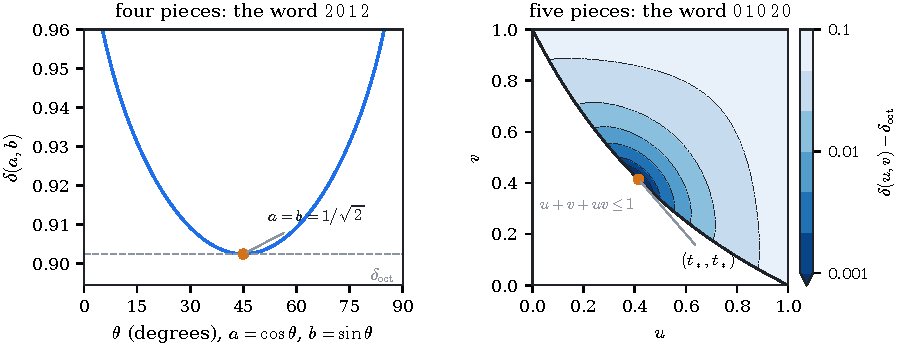
\includegraphics[width=\textwidth]{figures/fig-terminal-densities.pdf}
 \caption{Left: the four-piece density $\delta(\cos\theta,\sin\theta)$ of
 \eqref{eq:four-density}; its minimum $\doct$ is attained only at $\theta=45^\circ$, the octagon.
 Right: the excess $\delta(u,v)-\doct$ of the five-piece density \eqref{eq:five-density} over its
 domain $u,v\in(0,1)$, $u+v+uv>1$, on a logarithmic colour scale; it is positive everywhere and
 tends to $0$ only at the boundary point $(t_*,t_*)$, $t_*=\sqrt2-1$, where the middle factor
 tends to $1$. Both are computed from the cycle data; the script also checks the closure, the
 forced margins and the cost identity at random parameters.}
 \label{fig:terminal-densities}
\end{figure}

\begin{corollary}\label{cor:four-equality}
A closed vertex cycle with four pieces has raw cost at least $8\doct$. If its raw cost is
$8\doct$, then every factor is $\sqrt2$, every switch is forward, and its initial margins are
those of the octagon: the active margin $m_0(i_0)$ and the margin $m_0(i_0+2)$ equal
$2/\sqrt{2\sqrt2-1}$, and $m_0(i_0+1)=2(\sqrt2-1)/\sqrt{2\sqrt2-1}$.
\end{corollary}

\begin{proof}
Relabel to the word $2\,0\,1\,2$ and apply \cref{lem:four-param} and \cref{thm:four-density}. At
equality $a=b=1/\sqrt2$, so every factor is $\sqrt2$, $s=\sqrt2$, $\mathcal N=2\sqrt2-1$, and
\eqref{eq:four-margins} gives the stated margins.
\end{proof}

With active margin $a_k=2/\sqrt{2\sqrt2-1}$ and factor $\sqrt2$, each piece lasts
$(a_k/2)\log q_k=\log2/(2\sqrt{2\sqrt2-1})$, the octagon's switching time $\tsw$.

\subsection{Five pieces}\label{sec:terminal-five}

By \cref{prop:terminal-words}, a five-piece cycle that is not entirely reverse can be rebased
and relabeled to the word $0\,1\,0\,2\,0$, whose switches have the signs $+--++$. Its closure has
a two-parameter family of solutions. Put
\[
 P(t)=\frac{1+t^2}{2t},\qquad Q(t)=\frac{1+t^2}{1-t^2}\qquad(0<t<1).
\]

\begin{lemma}[Five-piece closure]\label{lem:five-closure}
If $p,q,r,s,z>1$ and
\[
 \widetilde T_0(p)\,\widetilde T_1(q)\,\widetilde T_0(r)\,\widetilde T_2(s)\,\widetilde T_0(z)
 =\widetilde R,
\]
then $p^2(q^2-1)=q^2$, $z^2(s^2-1)=s^2$ and $r^2=(q^2-1)(s^2-1)$. Consequently there are $u,v\in(0,1)$ with $u+v+uv>1$ and
\[
 (p,q,r,s,z)=\Bigl(P(u),\ Q(u),\ \frac{4uv}{(1-u^2)(1-v^2)},\ Q(v),\ P(v)\Bigr).
\]
\end{lemma}

\begin{proof}
The three relations come from the entries of the product compared with $\widetilde R$. Every
$q>1$ is $Q(u)$ for $u=\sqrt{(q-1)/(q+1)}\in(0,1)$, and then $p^2=q^2/(q^2-1)$ gives $p=P(u)$;
likewise for $s,z$ and $v$, and $r^2=(Q(u)^2-1)(Q(v)^2-1)$ gives the middle factor. Finally $r>1$
is equivalent to $u+v+uv>1$ by the factorization
$4uv-(1-u^2)(1-v^2)=(u+v+uv-1)(u+v+1-uv)$, whose second factor is positive.
\end{proof}

Put $d=(1-u)(1-v)$ and
\[
 F(t)=\Bigl(\frac{1+t}{1-t}\Bigr)^{2}\log\frac{1+t^2}{2t}+\frac{1}{t^2}\log\frac{1+t^2}{1-t^2}
 +\log\frac{2t}{1-t^2},
\]
and define the \emph{five-piece density}
\begin{equation}\label{eq:five-density}
 \delta(u,v)=\frac{2(d+2)-\tfrac{d}{2}\bigl(F(u)+F(v)\bigr)}{4-d}.
\end{equation}

\begin{lemma}[Five-piece cycles]\label{lem:five-param}
Let $c$ be a closed vertex cycle with word $0\,1\,0\,2\,0$. There are $u,v\in(0,1)$ with
$u+v+uv>1$ such that the factors are those of \cref{lem:five-closure}, the initial margins are
\[
 (m_0(0),m_0(1),m_0(2))=\frac{2}{\sqrt{d(4-d)}}\bigl((1+u)(1-v),\ d,\ (1-u)(1+v)\bigr),
\]
and the raw cost is $8\,\delta(u,v)$.
\end{lemma}

\begin{proof}
As for four pieces, the twist gives two linear equations for the initial margins, which the
quadric normalizes. With $A=(1+u)(1-v)$ and $B=(1-u)(1+v)$, the active margins of the five pieces
are $A$, $d/u$, $d$, $d/v$, $B$, times $2/\sqrt{d(4-d)}$. The algebraic part of the raw cost (all
but the terms $-a_k^2\log q_k$) adds up to $16\,d(d+2)/(d(4-d))$, and the logarithmic part is
\[
 -\frac{4}{d(4-d)}\Bigl(A^2\log P(u)+\frac{d^2}{u^2}\log Q(u)+d^2\log r+\frac{d^2}{v^2}\log Q(v)
 +B^2\log P(v)\Bigr).
\]
Since $A/d=(1+u)/(1-u)$, $B/d=(1+v)/(1-v)$ and
$\log r=\log\frac{2u}{1-u^2}+\log\frac{2v}{1-v^2}$, the bracket is $d^2(F(u)+F(v))$, and the
raw cost is $8\delta(u,v)$.
\end{proof}

\begin{theorem}[The five-piece density]\label{thm:five-density}
For $u,v\in(0,1)$ with $u+v+uv>1$, $\delta(u,v)>\doct$.
\end{theorem}

The proof is in \cref{app:five-density}; here is its structure. The function $F$ enters only
through $F(t)+2\log(1-t)$, and this function of one variable is at most its value at
$t_*=\sqrt2-1$, namely $(3+2\sqrt2)\log2+2\log(2-\sqrt2)$. Summing over
$t=u,v$ bounds $F(u)+F(v)$ above by a function of $d$ alone, hence $\delta(u,v)$ below by a
function of $d$. The constraint $u+v+uv>1$ gives $d<d_*=(2-\sqrt2)^2$, and at $d=d_*$ the lower
bound equals $\doct$ exactly. A tangent-line estimate for $d\log d$ at $d_*$ shows that the bound
exceeds $\doct$ for $d<d_*$. The infimum of $\delta(u,v)$ is approached only as $u,v\to t_*$,
where $d\to d_*$ and the middle factor $r$ tends to~$1$: the five-piece period degenerates into
the octagon's four pieces (right panel of \cref{fig:terminal-densities}).

\subsection{The terminal theorem}\label{sec:terminal-theorem}

\begin{proof}[Proof of \cref{thm:terminal}]
Let $c$ be the cycle of the period (\cref{lem:term-cycle}). It is not entirely reverse, by
\cref{thm:class-R}, which holds for every number of pieces. By \cref{prop:terminal-words}, either
it has four pieces, and then its raw cost is at least $8\doct$ by \cref{cor:four-equality}, or it
has five pieces and is a rebasing and relabeling of a cycle with word $0\,1\,0\,2\,0$, whose raw
cost exceeds $8\doct$ by \cref{lem:five-param} and \cref{thm:five-density}. By
\cref{lem:term-cycle},
$\cost\ge\frac{\sqrt3}{4}\cdot8\doct=\sqrt{12}\,\doct=\Aoct$.
\end{proof}

No competitiveness and no compact domain are needed here. The equality case identifies the
trajectory itself.

\begin{proof}[Proof of \cref{prop:terminal-equality}]
A five-piece cycle that is not entirely reverse has raw cost strictly above $8\doct$, and the
entirely reverse case is excluded by \cref{thm:class-R}, so $N=4$. By \cref{cor:four-equality} the period has four forward pieces,
all factors $\sqrt2$, and the octagon's initial margins. A traceless matrix is determined by its
margins, so after relabeling by a power of $R$ the initial state is $\Phi(0,y_0)$ with
$y_0^2=(2\sqrt2-1)/3$, and the control agrees almost everywhere with the octagon's control
$\ee_2\ee_0\ee_1\ee_2$ on four pieces of length $\tsw$. Changing a control on a null set does not
change a Carath\'eodory solution, and the octagon's trajectory is the unique solution with
$g(0)=I$ and $X(0)=\Phi(0,y_0)$, by uniqueness of solutions of the state equations with a fixed
vertex control on each piece.
\end{proof}

\subsection{The four- and five-piece estimates}\label{app:terminal-estimates}

This subsection proves \cref{thm:four-density,thm:five-density}. The four-piece comparison uses
monotonicity of a logarithmic weight; the five-piece comparison uses a concave integral kernel.

\subsubsection{A logarithm bound}\label{app:log-bound}

\begin{lemma}\label{lem:log-sinh}
For $0<x\le1$, $\ \dfrac{x-x^{-1}}{2}\le\log x$.
\end{lemma}

\begin{proof}
With $y=-\log x\ge0$ the inequality reads $y\le\sinh y$. The difference $\sinh y-y$ vanishes
at $0$ and has derivative $\cosh y-1\ge0$.
\end{proof}

\subsubsection{The four-piece density}\label{app:four-density}

Recall $\delta(a,b)$ from \eqref{eq:four-density}, on the open quarter circle $a,b>0$,
$a^2+b^2=1$, with $s=a+b$.

\begin{lemma}[A monotone weight]\label{lem:four-weight}
For $c\ge2$ the function $w_c(x)=(2x+c)\log x/(1-x)$ is nondecreasing on $(0,1)$. Consequently,
for $0<b\le a<1$,
\[
 (2b+c)(1-a)\log b\ \le\ (2a+c)(1-b)\log a.
\]
\end{lemma}

\begin{proof}
The derivative is $w_c'(x)=\bigl((2+c)\log x+(2x+c)(1-x)/x\bigr)/(1-x)^2$. By
\cref{lem:log-sinh} and $2+c>0$, the numerator is at least
\[
 (2+c)\frac{x-x^{-1}}{2}+\frac{(2x+c)(1-x)}{x}=\frac{(c-2)(1-x)^2}{2x}\ \ge\ 0.
\]
The second statement is $w_c(b)\le w_c(a)$ multiplied by $(1-a)(1-b)>0$.
\end{proof}

\begin{proof}[Proof of \cref{thm:four-density}]
Since $\delta(a,b)=\delta(b,a)$, we may assume $b\le a$, that is $b\in(0,1/\sqrt2\,]$ and
$a=\sqrt{1-b^2}$. Put $\psi(b)=\delta(\sqrt{1-b^2},b)$. For $0<b<1/\sqrt2$, differentiating
\eqref{eq:four-density} with $a'=-b/a$ and simplifying on the circle gives, with $c=2+2ab$,
\begin{equation}\label{eq:four-derivative}
 \psi'(b)=\frac{2\Bigl((s+1)\bigl(w_c(b)-w_c(a)\bigr)-s(s-1)(a-b)\Bigr)}{a\,(s+1)\,(s+3)^2}.
\end{equation}
Here $c\ge2$ and $b<a$, so $w_c(b)\le w_c(a)$ by \cref{lem:four-weight}, while $s>1$ and $a>b$
make the last term negative. Hence $\psi'<0$ on $(0,1/\sqrt2)$, and $\psi$, which is continuous
at $1/\sqrt2$, is strictly decreasing on $(0,1/\sqrt2\,]$. For $b<1/\sqrt2$ this gives
$\delta(a,b)=\psi(b)>\psi(1/\sqrt2)=\doct$, the value computed after \cref{thm:four-density}.
So $\delta(a,b)\ge\doct$ with equality only at $a=b$.
\end{proof}

\subsubsection{The five-piece density}\label{app:five-density}

Recall $F$, $d=(1-u)(1-v)$ and $\delta(u,v)$ from \eqref{eq:five-density}, and put
$t_*=\sqrt2-1$, $d_*=(2-\sqrt2)^2$ and $\mathcal K=(3+2\sqrt2)\log2$. Since
$(3+2\sqrt2)(2-\sqrt2)^2=2$, we have $\mathcal K d_*=2\log2$.

We locate the maximum of $F$ after a change of variables that splits it into two values of one
concave function at two points of the unit circle.

\begin{lemma}[A concave function]\label{lem:five-h}
Let $h(t)=-2t\log t/(1-t)-\log(1+t)$ for $0<t<1$. Then $x\mapsto h(\sqrt x)$ is strictly concave on
$(0,1)$. Consequently $h(\alpha)+h(\beta)\le2h(1/\sqrt2)$ whenever $\alpha,\beta>0$ and
$\alpha^2+\beta^2=1$, with equality only at $\alpha=\beta$.
\end{lemma}

\begin{proof}
The logarithmic remainder has the integral representation
\[
 t-1-\log t=(1-t)^2\int_0^1\frac{s}{1-s+st}\,\dd s.
\]
Differentiate $h$ and use this identity to obtain
\[
 \frac{h'(t)}{t}
 =2\int_0^1\frac{s}{1+t}\,\frac{1-s+s/t}{1-s+st}\,\dd s.
\]
For each fixed $s\in(0,1]$, the numerator $1-s+s/t$ decreases with $t$, and both positive
denominator factors increase. Thus the integrand, and hence $h'(t)/t$, strictly decreases on
$(0,1)$. The derivative of $h(\sqrt x)$ is $h'(\sqrt x)/(2\sqrt x)$, so this function is strictly
concave. Apply its midpoint inequality at $\alpha^2$ and $\beta^2$:
\[
 \tfrac12h(\alpha)+\tfrac12h(\beta)
 \le h\bigl(\sqrt{(\alpha^2+\beta^2)/2}\bigr)=h(1/\sqrt2),
\]
with equality only when $\alpha^2=\beta^2$.
\end{proof}

\begin{lemma}[The envelope]\label{lem:five-envelope}
For $0<t<1$,
\[
 F(t)+2\log(1-t)\ \le\ \mathcal K+2\log(2-\sqrt2)=\mathcal K+\log d_*.
\]
\end{lemma}

The bound is attained at $t=t_*$: there $(1+t^2)/(2t)=(1+t^2)/(1-t^2)=\sqrt2$,
$2t/(1-t^2)=1$ and $(1+t)/(1-t)=1/t=\sqrt2+1$, so $F(t_*)=(3+2\sqrt2)\log2=\mathcal K$, and
$1-t_*=2-\sqrt2$.

\begin{proof}
With $\alpha=2t/(1+t^2)$ and $\beta=(1-t^2)/(1+t^2)$, so that $\alpha^2+\beta^2=1$, expanding
the logarithms of the products $1-\alpha=(1-t)^2/(1+t^2)$, $1+\alpha=(1+t)^2/(1+t^2)$,
$1-\beta=2t^2/(1+t^2)$ and $1+\beta=2/(1+t^2)$ gives the identity
\[
 F(t)+2\log(1-t)=\log2+h(\alpha)+h(\beta).
\]
By \cref{lem:five-h} this is at most $\log2+2h(1/\sqrt2)$. Since $\log(1/\sqrt2)=-\tfrac12\log2$
and $1+1/\sqrt2=(2+\sqrt2)/2=1/(2-\sqrt2)$,
\[
 h(1/\sqrt2)=\frac{\sqrt2\cdot\tfrac12\log2}{1-1/\sqrt2}-\log\frac{1}{2-\sqrt2}
 =(1+\sqrt2)\log2+\log(2-\sqrt2),
\]
so $\log2+2h(1/\sqrt2)=(3+2\sqrt2)\log2+2\log(2-\sqrt2)$.
\end{proof}

\begin{lemma}\label{lem:five-d}
If $u,v\in(0,1)$ and $u+v+uv>1$, then $d=(1-u)(1-v)<d_*$.
\end{lemma}

\begin{proof}
Put $x=1-u$, $y=1-v$ and $\omega=\sqrt{xy}\in(0,1)$. The hypothesis is $(2-x)(2-y)>2$.
Since $x+y\ge2\omega$ by the arithmetic--geometric mean inequality,
\[
 (2-\omega)^2\ge(2-x)(2-y)>2.
\]
Thus $2-\omega>\sqrt2$, giving $d=\omega^2<(2-\sqrt2)^2=d_*$.
\end{proof}

\begin{proof}[Proof of \cref{thm:five-density}]
Adding \cref{lem:five-envelope} at $t=u$ and $t=v$, and using
$\log d=\log(1-u)+\log(1-v)$,
\[
 F(u)+F(v)\le2\mathcal K+2\log d_*-2\log d .
\]
Multiplying by $d/2>0$,
\[
 (4-d)\,\delta(u,v)=2d+4-\tfrac d2\bigl(F(u)+F(v)\bigr)\ \ge\ 2d+4-\mathcal Kd-d\log d_*+d\log d .
\]
The tangent line of $d\mapsto d\log d$ at $d_*$ gives $d\log d\ge d\log d_*+d-d_*$ (this is
$\log(d/d_*)\ge1-d_*/d$), so
\[
 (4-d)\,\delta(u,v)\ \ge\ 4-d_*+(3-\mathcal K)\,d .
\]
At $d=d_*$ the right side equals $\doct(4-d_*)$: indeed $2d_*+4-\mathcal Kd_*=16-8\sqrt2-2\log2$
and $4-d_*=2(2\sqrt2-1)$. Subtracting $\doct(4-d)=\doct(4-d_*)+\doct(d_*-d)$,
\[
 (4-d)\bigl(\delta(u,v)-\doct\bigr)\ \ge\ (\mathcal K-3-\doct)(d_*-d).
\]
The factor $d_*-d$ is positive by \cref{lem:five-d}. For the other factor put $r=\sqrt2$.
The strict midpoint inequality for the convex function $x\mapsto1/x$ on $[1,r]$ gives
\[
 \log2=2\int_1^r\frac{\dd x}{x}>\frac{4(r-1)}{r+1}.
\]
Using $r^2=2$ and the exact value of $\doct$, we obtain
\[
 (2r-1)(\mathcal K-3-\doct)
 =2(1+r)^2\log2-5-2r
 >8-5-2r=(r-1)^2>0.
\]
Since $4-d>0$, this proves $\delta(u,v)>\doct$.
\end{proof}

\begin{figure}[htbp]
 \centering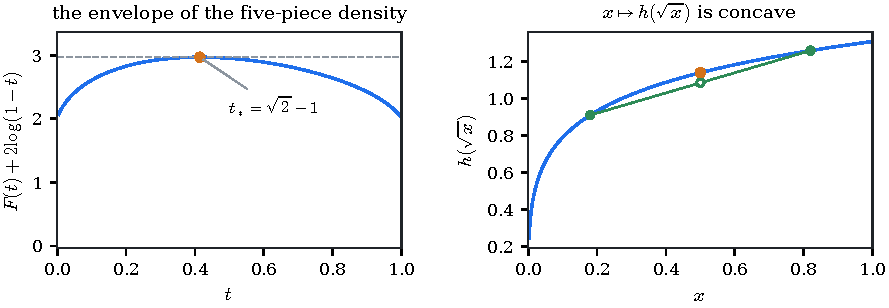
\includegraphics[width=\textwidth]{figures/fig-terminal-envelope.pdf}
 \caption{Left: $F(t)+2\log(1-t)$ on $(0,1)$; its maximum
 $(3+2\sqrt2)\log2+2\log(2-\sqrt2)$ is attained only at $t_*=\sqrt2-1$
 (\cref{lem:five-envelope}). Right: the concave function $x\mapsto h(\sqrt x)$ of
 \cref{lem:five-h}; a chord (green) lies below the graph, and the midpoint of the chord between
 $\alpha^2$ and $\beta^2=1-\alpha^2$ lies below the value at $x=1/2$ (orange). Computed; the
 script checks the identity $F(t)+2\log(1-t)=\log2+h(\alpha)+h(\beta)$ and the concavity on a
 grid.}
 \label{fig:terminal-envelope}
\end{figure}

\section{The equality case}\label{sec:equality}

\Cref{prop:terminal-equality} identifies a period of cost $\Aoct$ with the octagon's trajectory,
but only after three choices that the proof of the lower bound made along the way: the
normalization of the disk to Reinhardt's normal position, the rebasing of its trajectory at a
switch, and a relabeling of the vertices of the control simplex by a power of $R$. To classify the
disks of density $\doct$ these choices must be undone, and the trajectory to which the terminal
equality is applied must be the realization of the given disk; another minimizer of the same
cost would say nothing about it. This section carries the identification back to the disk
(\cref{sec:equality-rigidity}), proves the converse (\cref{sec:equality-converse}), identifies
Hales's octagon $\KH$ with Reinhardt's $\Koct$ (\cref{sec:equality-construction}). These results
complete the proofs of \cref{thm:main}(a) and~(c) in \cref{sec:equality-proofs}.

\subsection{Rigidity}\label{sec:equality-rigidity}

Let $s_0,\dots,s_5$ be the sixth roots of unity, so that $Rs_j=s_{j+1}$. The realization of a worst
disk (\cref{thm:equivalence}) keeps the link between its frame and its boundary.

\begin{lemma}[Realization with its contact link]\label{lem:eq-realization}
Let $K$ be a worst disk. There are an invertible linear map $e$ of the plane, a balanced pair
$\sigma$ of $eK$ in circle representation and a global minimizer $(T,u,g,X)$ of the control
problem such that $eK$ is a worst disk, $\delta(K)=\cost(T,X)/\sqrt{12}$, and for every $j$ and
every $t\in\R$
\[
 \sigma_j(t)=g(t)\,s_j,\qquad \sigma_j(t+T)=\sigma_{j+1}(t).
\]
\end{lemma}

The first identity is the definition of the frame of the realization, which is defined on all
of $\R$; the second is the cyclic shift of the contacts by one sixth of the period. Together they
force the frame to be twisted on all of $\R$, beyond the period $[0,T]$ on which the control
problem is posed.

\begin{lemma}[The frame twist]\label{lem:eq-frame-twist}
If $\sigma_j(t)=g(t)s_j$ and $\sigma_j(t+T)=\sigma_{j+1}(t)$ for all $j$ and $t$, then
$g(t+T)=g(t)R$ for every $t\in\R$.
\end{lemma}

\begin{proof}
$g(t+T)s_j=\sigma_j(t+T)=\sigma_{j+1}(t)=g(t)s_{j+1}=g(t)Rs_j$, and $s_0,s_1$ span the plane.
\end{proof}

The last ingredient recovers a disk from its boundary.

\begin{lemma}\label{lem:eq-frontier}
Two compact convex sets with nonempty interior, both symmetric about the origin, that have the
same frontier are equal.
\end{lemma}

\begin{proof}
Let $A,B$ be the two sets. The interior of $B$ is connected, contains the origin, and does not
meet the common frontier; it is covered by the disjoint open sets $\inter A$ and
$\R^2\setminus\overline A$, so it lies in $\inter A$, which contains the origin. By symmetry the
interiors are equal, and a convex body is the closure of its interior.
\end{proof}

\begin{proof}[Proof of \cref{thm:rigidity}]
Let $K$ be a worst disk, and take $e$, $\sigma$ and $(T,u,g,X)$ as in \cref{lem:eq-realization}.
By \cref{lem:eq-frame-twist}, $g(t+T)=g(t)R$ on $\R$.

\emph{The cost is $\Aoct$.} Since $K$ is a worst disk and $\delta(\KH)=\doct$
(\cref{prop:octagon-trajectory}), $\delta(K)\le\doct$, and part~(b) of \cref{thm:main} gives
$\delta(K)\ge\doct$. Hence $\cost(T,X)=\sqrt{12}\,\delta(K)=\Aoct$.

\emph{The terminal equality.} By \cref{thm:finite-normal}, the minimizer rebased at some
$s\in[0,T)$ is a normal vertex period $P$ with the same terminal time and cost, whose state stays
in $\hstarstar$; its frame is $t\mapsto g(s)^{-1}g(s+t)$, because $g$ is already twisted. By
\cref{thm:at-most-five}, $P$ has at most five pieces, and by \cref{prop:terminal-equality},
$T=\tf$ and there is $r$ with $R^{-r}g(s)^{-1}g(s+t)R^{r}=g_{\mathrm{oct}}(t)$ for $t\in[0,T]$.
With $M=g(s)R^r$ this reads
\[
 g(s+t)=M\,g_{\mathrm{oct}}(t)\,R^{-r}\qquad(0\le t<T).
\]
Both sides satisfy $F(t+T)=F(t)R$: the left side by the twist of $g$, the right side because
$g_{\mathrm{oct}}(t+\tf)=g_{\mathrm{oct}}(t)R$ and $R$ commutes with $R^{-r}$. Two curves with the
same twist that agree on $[0,T)$ agree everywhere, so the identity holds for all $t\in\R$.

\emph{The arcs.} Applying it to $s_0$ and using $R^{-r}s_0=s_{-r}$,
\[
 \sigma_0(s+t)=M\,g_{\mathrm{oct}}(t)\,s_{-r}=M\,\sigma^{\mathrm{oct}}_{-r}(t)\qquad(t\in\R),
\]
where $\sigma^{\mathrm{oct}}_j(t)=g_{\mathrm{oct}}(t)s_j$ are the contact curves of the octagon.
In a balanced pair each contact curve traces the whole frontier once per period, so the frontier
of $eK$ is the range of $\sigma_0$, and the frontier of $\KH$ is the range of
$\sigma^{\mathrm{oct}}_{-r}$. Hence $\partial(eK)=M(\partial\KH)=\partial(M\KH)$. Both $eK$ and
$M\KH$ are convex disks symmetric about the origin, so $eK=M\KH$ by \cref{lem:eq-frontier}, and
$K=e^{-1}M(\KH)$.
\end{proof}

The proof never compares $K$ with a minimizer other than its own realization. It runs the
reduction of \crefrange{sec:reduction}{sec:terminal} a second time, on that realization, and uses
the lower bound only to know that its cost is $\Aoct$.

\subsection{The converse}\label{sec:equality-converse}

The converse is the affine invariance of the greatest packing density.

\begin{proof}[Proof of \cref{prop:converse}]
A translate, and more generally a congruent copy, of $K$ has the same packings by congruent copies,
so its greatest packing density is the same. By
Fejes T\'oth's theorem (\cref{thm:fejes-toth}), $\delta(K)$ is the greatest density
$\operatorname{area}(K)/\det\Lambda$ of a lattice packing $K+\Lambda$. If $\det A>0$, the
lattice packings of $K$ and of $AK$ correspond through $\Lambda\mapsto A\Lambda$, and area and
covolume are both multiplied by $\det A$, so the lattice densities agree. If $\det A<0$, write
$A=(AF)F$ with the reflection $F(x_0,x_1)=(x_0,-x_1)$: then $FK$ is a congruent copy of $K$, and
$AF$ preserves orientation. The last statement follows from $\delta(\KH)=\doct$
(\cref{prop:octagon-trajectory}).
\end{proof}

\subsection{Reinhardt's construction}\label{sec:equality-construction}

\Cref{thm:main} is stated for Reinhardt's octagon $\Koct$ (\cref{def:smoothed-octagon}), while
the proof works with $\KH$, the region swept from the origin by the contact curve
$\sigma^{\mathrm{oct}}_0$ of the octagon's trajectory over one period $[0,6\tf]$. By
\cref{prop:octagon-trajectory}, $\KH$ is also the convex hull of the six arcs
$\sigma^{\mathrm{oct}}_j([0,\tf])$. The two octagons differ by a vertical stretch of about $5.5\%$
(\cref{fig:octagon}).

\begin{proof}[Proof of \cref{prop:reinhardt-construction}]
Write $y_0^2=(2\sqrt2-1)/3$ and $W=\exp(\sqrt3\,y_0 s)$ for $s\in[0,\tsw]$, so that $W$ runs over
$[1,\sqrt2]$; recall that $\sigma^{\mathrm{oct}}_0(0)=s_0=(1,0)$.

\emph{One eighth of the boundary.} On the first switching interval the octagon's frame
$g_0(s)$ is the flow of the control $\ee_2$ from $\Phi(0,y_0)$; conjugated by $A$ it acts by
\[
 Ag_0(s)A^{-1}=\begin{pmatrix}1&-\frac{W-1}{2\sqrt2-1}\\[0.5ex]
 1-W^{-1}&1-\frac{W-2+W^{-1}}{2\sqrt2-1}\end{pmatrix},
\]
and $A\,g_0(\tsw)R^{-1}A^{-1}$ is the rotation by $-\pi/4$; both are direct computations from
the closed form of the flow of $\ee_2$. Since $g_{\mathrm{oct}}(t+\tsw)=g_0(\tsw)R^{-1}\,g_{\mathrm{oct}}(t)\,R$,
the curve $A\sigma^{\mathrm{oct}}_0$ is, on the first three switching intervals,
\begin{align*}
 &(1,\ 1-W^{-1}) &&\text{along side $0$},\\
 &\Bigl(\sqrt2+1-\tfrac{\sqrt2}{2}(W+W^{-1}),\ 1-\tfrac{\sqrt2}{2W}\Bigr)
  &&\text{around corner $0$},\\
 &\Bigl(\sqrt2-\tfrac W2,\ \tfrac W2\Bigr) &&\text{along side $1$}.
\end{align*}
The first piece runs from the midpoint $(1,0)$ of side~$0$ to the point $(1,1-\sqrt2/2)$, and the
third from $(\sqrt2-\tfrac12,\tfrac12)$ to the midpoint $(\sqrt2/2,\sqrt2/2)$ of side~$1$.
With $d_k$ the distance to the $k$th side line, the middle piece has $d_7=W/2$ and
$d_2=\sqrt2/(2W)$, so it lies on the hyperbola $d_7d_2=\sqrt2/4$; it starts at
$(1,1-\sqrt2/2)$ and ends at $(\sqrt2-\tfrac12,\tfrac12)$, the points where the first and the
third pieces end and start. The control on these three intervals is $\ee_2$, $\ee_0$, $\ee_1$,
and only the second bends the curve.

\emph{The rest.} Three switching intervals later the frame relation gives
$\sigma^{\mathrm{oct}}_0(t+3\tsw)=-h^3\sigma^{\mathrm{oct}}_0(t)$ with $h=g_0(\tsw)R^{-1}$, and
$-Ah^3A^{-1}$ is the rotation by $\pi/4$. Over the period
$6\tf=24\tsw$ the curve $A\sigma^{\mathrm{oct}}_0$ therefore traces eight rotated copies of the
three pieces, once around.

\emph{The two inclusions.} Every point $q$ of the three pieces lies in $\Koct$, and $\mu q$ does
not for $\mu>1$: on the sides this is the inequality $d_k\ge0$, and on the corner it is the
hyperbola condition, which strictly fails past the arc. Since $\Koct$ is invariant under the
rotation by $\pi/4$, the same holds for every point $A\sigma^{\mathrm{oct}}_0(t)$. The set $\Koct$ is star-shaped about $0$, so $A\KH\subseteq\Koct$.
Conversely, a point $p\ne0$ of $\Koct$ is a positive multiple $\lambda q$ of some
$q=A\sigma^{\mathrm{oct}}_0(t)$, by the intermediate value theorem and
$\sigma^{\mathrm{oct}}_0(t+3\tf)=-\sigma^{\mathrm{oct}}_0(t)$, and $\lambda\le1$ because
$\mu q\notin\Koct$ for $\mu>1$. Hence $p\in A\KH$.
\end{proof}

Each side of $\Koct$ keeps a straight middle part of length $2-\sqrt2$, between the points of
tangency $(1,\pm(1-\sqrt2/2))$ on side~$0$. The proposition transfers the facts known for $\KH$ to
$\Koct$; in particular, the affine images of the two octagons are the same sets.

\section{The formal verification}\label{app:formal}

The formalization of the main theorems uses Lean~4~\cite{Lean4} and Mathlib~\cite{Mathlib20} and
is available in the repository~\cite{Companion}. We describe its statements, verification and
dependencies, then give the correspondence between the paper and the Lean declarations.

\subsection{The statements}\label{app:formal-statements}

The file \texttt{Palomar/Challenge.lean} imports only Mathlib and states the three parts of
\cref{thm:main} as the theorems \lean{octagon_density}, \lean{reinhardt} and
\lean{reinhardt_equality} of the namespace \lean{ReinhardtChallenge}. Its packing definitions
agree with \cref{def:packing-density}, which is Definition~2.1.1 of~\cite{HalesVajjha2024}. Points
of the plane are maps $\{0,1\}\to\R$ and areas are Lebesgue measure. A convex disk is a compact
convex set with nonempty interior, and a congruent copy of $K$ is its image under a map $x\mapsto
Ax+b$ with $A$ orthogonal. A packing is a family of convex disks with pairwise disjoint interiors.
Its density exists when the upper and lower limits, as $r\to\infty$, of the covered fraction of
the disk of radius $r$ about the origin are finite and equal. The greatest packing density
$\delta(K)$ is the supremum over packings by congruent copies of $K$ for which this density
exists. A disk is centrally symmetric when there is a point $c$ with $2c-x\in K$ for every $x\in
K$. The smoothed octagon is given in Reinhardt's description (\cref{def:smoothed-octagon}): with
$d_k(x)$ the signed distance from $x$ to the line of the $k$-th side of the regular octagon of
inradius~$1$, it is the octagon $d_k\ge0$ with the corner between sides $k$ and $k+1$ cut off
along the hyperbola $d_{k-1}d_{k+2}=\sqrt2/4$. The definitions are copied verbatim from the
library, so the library's theorems have precisely the statements given in the challenge file.

\subsection{Verification and dependencies}\label{app:formal-check}

The three theorems are proved without additional hypotheses in the root module
\texttt{SmoothedOctagon.lean}. Lean's kernel checks the proofs. Every theorem depends only on the
standard axioms \lean{propext}, \lean{Classical.choice} and \lean{Quot.sound}, as verified by an
audit of every declaration in the library. The Comparator configuration
\texttt{Palomar/comparator.json} checks that the root module proves the statements of
\texttt{Palomar/Challenge.lean} with the same definitions. The proof is registered in the Palomar
registry~\cite{Palomar} as \texttt{PALOMAR-2026-11-09-000008}, at trust level high: Palomar's
verifier checked it with the independent kernels nanoda and con-ron at commit \texttt{9ba6bf8}
of~\cite{Companion}. Lean and Mathlib are pinned at version \texttt{v4.36.0-rc2}. The library has
about 125{,}000 lines in 407 modules, and a full build takes about 3.5 CPU-hours.

The library depends on two others. The first~\cite{SmoothedPolygonLean} formalizes the parts of
the book of Hales and Vajjha~\cite{HalesVajjha2024} that the proof uses, together with the
classical results on which they depend, including Fejes T\'oth's theorem (\cref{thm:fejes-toth}),
the theorems of Minkowski and Mahler on critical lattices and circumscribed hexagons, the compact
domain (\cref{thm:compact-domain}) and the lift of a global minimizer to a Pontryagin extremal
(\cref{thm:pmp-lift}). The second~\cite{OptimalControlLean} proves the Pontryagin maximum
principle~\cite{Pontryagin1962} with free terminal time, an integral cost and mixed boundary
conditions, by the argument of Agrachev and Sachkov~\cite{AgrachevSachkov2004}, and Filippov's
theorem~\cite{Filippov1962}; Brouwer's fixed-point theorem comes from~\cite{FixedPointLean}.

\subsection{Dictionary}\label{app:formal-dictionary}

\Cref{tab:formal-dictionary} lists the Lean declarations corresponding to the numbered results and
constructions of the paper. Names are relative to the namespace \lean{SmoothedOctagon}; the
prefixes \lean{ReinhardtChallenge} and \lean{SmoothedPolygons} mark the statements of the
challenge file and the declarations of~\cite{SmoothedPolygonLean}. Multiple declarations in one
row jointly establish the corresponding result. The rows are grouped by the appendix that proves
the result; \cref{thm:main,thm:control} and the definitions of \cref{sec:setting} come first.

{\small
\begin{longtable}{@{}>{\raggedright\arraybackslash}p{0.25\textwidth}>{\raggedright\arraybackslash}p{0.71\textwidth}@{}}
\caption{The Lean declarations behind the numbered results.}\label{tab:formal-dictionary}\\
\toprule
Result & Lean declarations\\
\midrule
\endfirsthead
\toprule
Result & Lean declarations\\
\midrule
\endhead
\bottomrule
\endfoot
\multicolumn{2}{@{}l}{\emph{\Cref{sec:intro,sec:setting}}}\\*[2pt]
\cref{thm:control} & \lean{reinhardt_cost}, \lean{controlLowerBound} \\
\cref{thm:main}(a) & \lean{ReinhardtChallenge.octagon_density}, \lean{smoothedOctagon_spec} \\
\cref{thm:main}(b) & \lean{ReinhardtChallenge.reinhardt}, \lean{reinhardtConjecture} \\
\cref{thm:main}(c) & \lean{ReinhardtChallenge.reinhardt_equality}, \lean{reinhardt_equality_trajectory} \\
\cref{def:packing-density} & \lean{ReinhardtChallenge.greatestPackingDensity} \\
\cref{def:smoothed-octagon} & \lean{ReinhardtChallenge.smoothedOctagon} \\
\cref{def:global-minimizer} & \lean{SmoothedPolygons.IsReinhardtMinimizer} \\
\cref{thm:compact-domain} & \lean{SmoothedPolygons.theorem5_0_2} \\
\addlinespace
\multicolumn{2}{@{}l}{\emph{\Cref{sec:reduction}}}\\[2pt]
\cref{def:pmp-extremal} & \lean{SmoothedPolygons.IsPontryaginExtremal} \\
\cref{thm:pmp-lift} & \lean{SmoothedPolygons.exists_isPontryaginExtremal_of_isReinhardtMinimizer} \\
\cref{lem:vertex-hamiltonians} & \lean{IsPontryaginExtremal.continuousOn_vertexHamiltonian}, \lean{IsPontryaginExtremal.vertexHamiltonian_max_eq_zero} \\
\cref{red:singular-locus} & \lean{hamiltonian_vertices_equal_iff_reducedCostate_eq_zero}, \lean{hamiltonian_maximizers_in_proper_edge} \\
\cref{red:winding} & \lean{Reduction.clr_winding}, \lean{Reduction.clr_angular} \\
\cref{red:equilibrium} & \lean{Reduction.clr_vertex_bounds}, \lean{Reduction.clr_equilibrium_compact} \\
\cref{red:budget} & \lean{Reduction.clr_budget}, \lean{Reduction.clr_abs_lam_le}, \lean{Reduction.clr_lam_sq_le} \\
\cref{prop:clearance} & \lean{Reduction.covectorNormSq_le_singularGapSq}, \lean{Reduction.switch_singularGapSq_pos} \\
\cref{red:clearance-remark} & \lean{Reduction.clr_frobSq_frame_le}, \lean{Reduction.covectorNormSq_projective_bounds} \\
\cref{prop:edge-bound} & \lean{Reduction.edgeBound_of_isReinhardtMinimizer}, \lean{Reduction.Edge.edge_bangBang} \\
\cref{red:local-exclusion} & \lean{Reduction.switch_exists_excluded_vertex} \\
\cref{prop:finite-switches} & \lean{Reduction.exists_isPiecewiseVertex} \\
\cref{def:vertex-representation} & \lean{VertexRepresentation} \\
\cref{lem:word-reduction} & \lean{Reduction.exists_rebase_vertexRepresentation}, \lean{Reduction.isReinhardtMinimizer_rebase} \\
\cref{def:normal-period} & \lean{NormalPeriod}, \lean{NormalPeriod.IsCompetitive}, \lean{NormalPeriod.InCompactDomain}, \lean{NormalPeriod.activeMargin} \\
\cref{thm:normality} & \lean{Reduction.lam_lt_zero_of_vertexRepresentation}, \lean{Reduction.exists_normal_lift} \\
\cref{red:abnormal-transport} & \lean{Reduction.gn_piece} \\
\cref{thm:finite-normal} & \lean{finiteNormalRepresentation}, \lean{Reduction.cost_le_octagonCost} \\
\addlinespace
\multicolumn{2}{@{}l}{\emph{\Cref{sec:periods,sec:reverse,sec:mixed-runs}}}\\[2pt]
\cref{lem:one-arc} & \lean{vertexPiece_eq}, \lean{vertexPiece_margin}, \lean{vertexPiece_cost}, \lean{NormalPeriod.piece_margin}, \lean{NormalPeriod.cost_eq_sum} \\
\cref{lem:per-factors} & \lean{CostateCycle.factor_pp}, \lean{CostateCycle.factor_mp}, \lean{CostateCycle.factor_pm}, \lean{CostateCycle.centre_factor} \\
\cref{lem:per-signed-action} & \lean{CostateCycle.rawCost_eq}, \lean{CostateCycle.arc_eq}, \lean{NormalPeriod.cost_eq_rawCost} \\
\cref{lem:tangent-closure} & \lean{NormalPeriod.tangentProduct_N}, \lean{Term.triC_conj_tangentFactor}, \lean{Term.triC_conj_R} \\
\cref{def:signs} & \lean{VertexRepresentation.IsForward}, \lean{VertexRepresentation.IsReverse}, \lean{VertexRepresentation.IsReverseRun}, \lean{VertexRepresentation.IsForwardRun} \\
\cref{lem:sign-sum} & \lean{NormalPeriod.ff_N_mod_three} \\
\cref{def:classes} & \lean{VertexRepresentation.AllReverse}, \lean{VertexRepresentation.AllForward}, \lean{VertexRepresentation.ClassM3}, \lean{VertexRepresentation.ClassM1}, \lean{VertexRepresentation.ClassM2} \\
\cref{prop:partition} & \lean{VertexRepresentation.partition} \\
\cref{def:costate-coordinates} & \lean{costateL}, \lean{costateA}, \lean{costateB}, \lean{costateAlpha}, \lean{costateBeta}, \lean{CostateCycle.sig} \\
\cref{lem:costate-transport} & \lean{margin_mul_hamiltonian}, \lean{costateB_perp}, \lean{vertexPiece_costate}, \lean{NormalPeriod.cut_transport}, \lean{NormalPeriod.sig_le_of_mem}, \lean{NormalPeriod.cut_sig_grow_le}, \lean{NormalPeriod.cut_sig_decr_le}, \lean{CostateCycle.sig_act_succ}, \lean{NormalPeriod.costateCycle} \\
\cref{def:normal-multiplier} & \lean{NormalPeriod.Ucal}, \lean{CostateCycle.mu}, \lean{NormalPeriod.mu_zero}, \lean{CostateCycle.gam2}, \lean{NormalPeriod.det_Ucal}, \lean{triY}, \lean{CostateCycle.Mloc} \\
\cref{lem:per-switch-vectors} & \lean{CostateCycle.yv_norm}, \lean{CostateCycle.cross_pp}, \lean{CostateCycle.cross_mm}, \lean{CostateCycle.yv_pair}, \lean{CostateCycle.outv_turn}, \lean{CostateCycle.yv_add_N}, \lean{CostateCycle.pre_N} \\
\cref{lem:stationarity} & \lean{CostateCycle.stationarity}, \lean{CostateCycle.centre_stat} \\
\cref{lem:switch-norms} & \lean{CostateCycle.swd_fwd}, \lean{CostateCycle.swd_rev}, \lean{CostateCycle.turn_secant}, \lean{CostateCycle.turn_swd_ge} \\
\cref{lem:gram} & \lean{CostateCycle.gram_pp}, \lean{CostateCycle.gram_mm} \\
\cref{prop:ellipticity} & \lean{NormalPeriod.gam2_pos_of_mixed}, \lean{NormalPeriod.wire_gam2_pos_of_allForward} \\
\cref{prop:cost-casimir} & \lean{NormalPeriod.cost_casimir}, \lean{el_winding} \\
\cref{cor:casimir-cap} & \lean{NormalPeriod.gam2_lt_cap} \\
\cref{thm:at-most-five} & \lean{period_le_five} \\
\cref{lem:rev-N} & \lean{cstRevN_neg} \\
\cref{lem:rev-identities} & \lean{cst_rev4_third_identity}, \lean{cst_rev4_second_identity} \\
\cref{lem:reverse-four} & \lean{CostateCycle.reverse_four_third}, \lean{CostateCycle.reverse_four_second} \\
\cref{thm:class-R} & \lean{reverse_exclusion} \\
\cref{lem:three-arc} & \lean{CostateCycle.three_arc}, \lean{CostateCycle.three_arc_not_min}, \lean{CostateCycle.turn_up}, \lean{CostateCycle.turn_down}, \lean{cst_three_grow}, \lean{cst_three_decr} \\
\cref{prop:run-structure} & \lean{reverseRun_two_and_centre_min} \\
\cref{thm:class-M3} & \lean{minimumStructure_exclusion} \\
\cref{cor:rev-mixed} & \lean{NormalPeriod.rev_run}, \lean{NormalPeriod.centre_min}, \lean{NormalPeriod.swd_ge_of_mixed} \\
\cref{lem:rev-three-gram} & \lean{el_three_gram} \\
\cref{lem:rev-cross-signs} & \lean{CostateCycle.cre_pos_pp}, \lean{CostateCycle.cre_neg_mm}, \lean{el_cross_bound} \\
\cref{lem:rev-pade} & \lean{cst_log_pade}, \lean{cst_zeta_gt}, \lean{cst_eta_lt_zeta} \\
\cref{lem:octagon-cost-comparison} & \lean{octagonCost_ratio_lt}, \lean{octagon_moment_ratio_lt_golden}, \lean{octagonCost_lt_score} \\
\addlinespace
\multicolumn{2}{@{}l}{\emph{\Cref{sec:short-runs}}}\\[2pt]
\cref{thm:class-M1} & \lean{shortRuns_exclusion} \\
\cref{lem:m1-pattern} & \lean{VertexRepresentation.m1_pattern} \\
\cref{lem:m1-centre-data} & \lean{NormalPeriod.m1_centreData}, \lean{m1_CentreData} \\
\cref{prop:m1-angle-gap} & \lean{m1_angle_gap} \\
\cref{cor:m1-angle} & \lean{m1_arccos_gt}, \lean{m1_cos_two_pi_div_five} \\
\cref{prop:m1-winding} & \lean{m1_winding}, \lean{wind_winding_aux}, \lean{wind_polar}, \lean{wind_centre}, \lean{wind_track_range}, \lean{wind_seam} \\
\cref{lem:m1-recurrence} & \lean{CostateCycle.m1_next_centre}, \lean{CostateCycle.next_centre_local}, \lean{CostateCycle.cross_mm}, \lean{CostateCycle.pre_N} \\
\cref{lem:m1-euler} & \lean{CostateCycle.euler_sum}, \lean{CostateCycle.rawCost_eq}, \lean{elGa_euler} \\
\cref{prop:m1-two-centre} & \lean{m1_two_centre}, \lean{m1_two_centre_bounds}, \lean{m1_octagonCost_lt_two_centre} \\
\cref{lem:m1-log} & \lean{ag_half_sub_inv_le_log}, \lean{ag_sigma_superadd} \\
\cref{lem:m1-one-switch} & \lean{ag_phi_le} \\
\cref{lem:m1-reduce} & steps of the proof of \lean{m1_angle_gap} \\
\cref{lem:m1-symmetric} & \lean{agSymmetric_gram_min}, \lean{agSymRoot_existsUnique}, \lean{agSymRoot_zero_spec} \\
\cref{lem:m1-core} & \lean{ag_core} \\
\cref{lem:m1-bc} & \lean{m1_bc_bound} \\
\addlinespace
\multicolumn{2}{@{}l}{\emph{\Cref{sec:forward}}}\\[2pt]
\cref{thm:class-F} & \lean{forward_exclusion} \\
\cref{lem:fwd-count} & \lean{NormalPeriod.ff_N_mod_three} \\
\cref{lem:fwd-cycle} & \lean{CostateCycle.ff_act_mul_lt}, \lean{CostateCycle.ff_q_eq}, \lean{CostateCycle.ff_rawCost} \\
\cref{lem:fwd-seven} & \lean{ff_seven_le} \\
\cref{prop:fwd-window} & \lean{CostateCycle.ff_rows}, \lean{CostateCycle.ff_floors}, \lean{CostateCycle.ff_gram}, \lean{NormalPeriod.ff_gam2_eq}, \lean{ff_Win.toDim} \\
\cref{prop:fwd-spectral} & \lean{NormalPeriod.ff_cost_casimir}, \lean{NormalPeriod.wire_gam2_pos_of_allForward}, \lean{NormalPeriod.wire_spectral} \\
\eqref{eq:spectral-subinterval} & \lean{NormalPeriod.df_angle} \\
\cref{cor:fwd-cap} & \lean{NormalPeriod.ff_competitive_cap_exact}, \lean{octagon_spectral_cap} \\
\cref{lem:fwd-small} & \lean{ff_Dim.U_lt_three}, \lean{fs_U_lt_three}, \lean{fs_H5P_pos} \\
\cref{lem:fwd-threshold} & \lean{ff_Dim.eleven_fifths_lt}, \lean{ff_octagonCost_lt_sqrt} \\
\cref{lem:fwd-joint-concavity} & \lean{ff_budgetCost_strictConcaveOn} \\
\cref{lem:fwd-budget} & \lean{ff_Dim.budget}, \lean{ff_Dim.h_le_c}, \lean{ff_budget_g}, \lean{ff_budget_linear} \\
\cref{lem:fwd-neighbour} & \lean{ff_Dim.neighbor}, \lean{ff_resN_neg} \\
\cref{lem:fwd-neighbour-value} & \lean{fs_neighborValue_neg}, \lean{fs_NS_Eval} \\
\cref{lem:fwd-neighbour-symmetric} & \lean{fs_neighborSlope_neg}, \lean{fs_NS_Dval}, \lean{fs_resN_sym_of_floor} \\
\cref{lem:fwd-neighbour-asymmetric} & \lean{asym_continuous_row_neg}, \lean{asym_original_row_neg}, \lean{fs_resN_asym} \\
\cref{lem:fwd-individual} & \lean{fs_normValue_neg}, \lean{fs_normTangent_neg}, \lean{fs_resV_neg}, \lean{fs_factor_curvature_nonneg} \\
\cref{lem:fwd-sum} & \lean{fwdSumPairedLog_le}, \lean{fwdSumResidual32_original_neg}, \lean{fs_resS_neg} \\
\cref{lem:fwd-norms} & \lean{ff_Dim.norms}, \lean{ff_Dim.norms_nonneg}, \lean{ff_resS_neg}, \lean{ff_resV_neg} \\
\cref{lem:fwd-casimir} & \lean{fcNormQ_polygon}, \lean{fc_branch_curve_gt}, \lean{fc_sum_curve_gt}, \lean{ff_casimir_lower} \\
\addlinespace
\multicolumn{2}{@{}l}{\emph{\Cref{sec:mixed}}}\\[2pt]
\cref{thm:class-M2} & \lean{nonshort_exclusion} \\
\cref{lem:m2-casimir} & \lean{NormalPeriod.wire_spectral}, \lean{NormalPeriod.wire_cas_lt}, \lean{NormalPeriod.dens_cas_gt} \\
\cref{lem:m2-scale} & \lean{m2_centre}, \lean{m2_scale} \\
\cref{prop:m2-small-forward} & \lean{m2_small_forward_minimum} \\
\cref{prop:m2-centre} & \lean{m2_min_centre} \\
\cref{lem:m2-reflection} & \lean{m2_reflect}, \lean{m2_reflect_fwd_iff}, \lean{m2_reflect_classM2} \\
\cref{prop:m2-window} & \lean{m2_window} \\
\cref{prop:m2-continuation} & \lean{m2_window}, \lean{M2Window.ForwardNext}, \lean{M2Window.ReverseNext} \\
\cref{lem:m2-comparison} & \lean{m2_comparison} \\
\cref{lem:m2-shape} & \lean{nsrN_mono_k}, \lean{nsrA_pos} \\
\cref{lem:m2-necessary} & \lean{nsr_window_basic}, \lean{nsr_window_N_neg}, \lean{nsr_high_t}, \lean{nsr_scale_lt}, \lean{nsr_scale_k}, \lean{nsr_scale_of_t}, \lean{nsr_centre_gap}, \lean{nsr_centre_gap_k}, \lean{nsr_window_dur}, \lean{nsr_window_dur_x}, \lean{nsr_reverse_order}, \lean{nsr_reverse_order_k} \\
\cref{prop:m2-reverse-core} & \lean{nsr_reverse_core} \\
\cref{thm:m2-reverse} & \lean{m2_reverse_exclusion} \\
\cref{prop:m2-forward-steps} & \lean{nsf_low_ratio}, \lean{nsf_small_gap_j}, \lean{nsf_small_gap} \\
\cref{thm:m2-forward} & \lean{m2_forward_exclusion} \\
\cref{lem:m2-secants} & \lean{nsr_sec_swap}, \lean{nsr_sec_start}, \lean{nsr_m2F_eq_sec}, \lean{nsr_sec_lt_chord}, \lean{nsr_turn_floor} \\
\cref{lem:m2-logs} & \lean{nsr_log_one_add_gt}, \lean{nsr_secN_lt_vbar}, \lean{nsr_log_lt_Lp}, \lean{nsr_m2F_gt_Fl}, \lean{mix_log_weighted_lt}, \lean{nsr_log_one_add_jensen}, \lean{nsr_secN_lt_jensen}, \lean{nsf_secN_lt_VG}, \lean{nsf_secN_lt_Vq}, \lean{nsr_t_lt_T} \\
\cref{lem:m2-relax} & \lean{nsrNv_nonpos}, \lean{nsrNL_nonpos}, \lean{nsr_N_pos_of_relax} \\
\cref{lem:m2-centre-gap} & \lean{nsr_centre_gap}, \lean{nsr_centre_gap_k}, \lean{nsr_gap_chord_pos}, \lean{nsr_gap_normalize} \\
\cref{lem:m2-high-t} & \lean{mhtDelta_physical_pos}, \lean{nsr_high_t_analytic}, \lean{nsr_high_t'} \\
\cref{lem:m2-unit-shape} & \lean{nsr_unit_shape}, \lean{nsr_cubic_pos}, \lean{nsrU_signs}, \lean{nsrUC0_pos} \\
\cref{lem:m2-order-face} & \lean{nsr_order_face}, \lean{nsr_q_le_order}, \lean{nsr_concave_min}, \lean{nsr_order_one_pos} \\
\cref{lem:m2-strip} & \lean{nsr_strip} \\
\cref{lem:m2-low-unit} & \lean{nsr_low_unit}, \lean{nsr_low_kh}, \lean{nsr_quartic_cubic_tail} \\
\cref{lem:m2-low-ratio} & \lean{nsf_lowRatio_core}, \lean{nlr_shape_mono}, \lean{nlr_unit_pos} \\
\cref{lem:m2-large-gap} & \lean{nsf_LGN_core}, \lean{nsf_LGB_core}, \lean{nlt_unit_pos}, \lean{nlt_shape_ge}, \lean{hrl_lower_pos}, \lean{hrs_shape_lt} \\
\cref{lem:m2-chi} & \lean{nsf_chi_core} \\
\cref{lem:m2-slope} & \lean{nsf_cas_slope} \\
\cref{lem:m2-qelim} & \lean{nsf_qelim} \\
\cref{lem:m2-envelope} & \lean{nsf_envelope}, \lean{nsf_wU_floor}, \lean{nsf_norm_derivative_neg} \\
\addlinespace
\multicolumn{2}{@{}l}{\emph{\Cref{sec:smaller-short}}}\\[2pt]
\cref{def:ss-window} & \lean{M2Short} \\
\cref{prop:ss-extraction} & \lean{m2_short_window} \\
\eqref{eq:ss-defect} & \lean{NormalPeriod.df_window}, \lean{NormalPeriod.df_defect} \\
\eqref{eq:ss-bridge-frame}, \eqref{eq:ss-angle-data} & \lean{df_alg_m}, \lean{df_alg_traces}, \lean{SmallerShort.Point.AA}, \lean{SmallerShort.Point.BB} \\
\cref{thm:m2-smaller-short} & \lean{m2_smallerShort_exclusion} \\
\cref{lem:ss-first} & \lean{M2Short.ss_C_le_B}, \lean{SmallerShortData.u_le_V}, \lean{ss_V_lt_limit}, \lean{M2Short.ss_u_le}, \lean{SmallerShortData.be_le_al_x}, \lean{SmallerShortData.root_zero}, \lean{SmallerShortData.q_le_qc}, \lean{SmallerShortData.q_lt_seventh} \\
\cref{app:ss-secant} & \lean{ss_V_lt_VG}, \lean{ss_V_le_Vbar}, \lean{mix_log_weighted_lt} \\
\cref{lem:ss-orders} & \lean{ss_strong_order}, \lean{ss_upper_order_54}, \lean{ss_upper_order_98}, \lean{ss_small_upper_order}, \lean{ss_quad_order}, \lean{SmallerShortData.strong_box} \\
\cref{prop:ss-S0} & \lean{M2Short.ratio_lt_twelve_fifths}, \lean{SmallerShortData.ratio_lt_twelve_fifths}, \lean{lgr_D_pos}, \lean{lgr_pairing} \\
\cref{prop:ss-S1} & \lean{M2Short.two_lt_ratio}, \lean{SmallerShortData.two_lt_ratio}, \lean{SmallerShortData.lr_cap_env} \\
\cref{prop:ss-S2} & \lean{M2Short.ratio_lt_thirteen_sixths}, \lean{SmallerShortData.ratio_lt_thirteen_sixths} \\
\cref{prop:ss-S3} & \lean{M2Short.displacement_lt}, \lean{SmallerShortData.displacement_lt} \\
\cref{prop:ss-S4} & \lean{M2Short.upper_order_casimir_floor}, \lean{SmallerShortData.upper_order_casimir_floor}, \lean{SmallerShortData.cas_cap_env} \\
\cref{prop:ss-S5} & \lean{M2Short.shear_neg}, \lean{SmallerShortData.shear_neg}, \lean{shr_residual_neg}, \lean{shr_shear_sign}, \lean{shr_norm_mono}, \lean{shr_small_shape_factor}, \lean{ss_A2_pos} \\
\cref{prop:ss-S6} & \lean{M2Short.octagonCost_lt_completion}, \lean{SmallerShortData.octagonCost_lt_completion}, \lean{SmallerShortData.cost_angle}, \lean{SmallerShortData.cost_continuation}, \lean{cost_Fc_gt}, \lean{octagonCost_lt_score} \\
\cref{lem:ss-first-contact} & \lean{ss_first_contact} \\
\cref{lem:ss-endpoint-gaps} & \lean{ss_gap_ratio_bounds}, \lean{ss_gap_ratio_tilted} \\
\cref{lem:ss-outer-scale} & \lean{ss_reverseGram_mono}, \lean{ss_rev_centre_scale} \\
\cref{prop:ss-face-S0} & \lean{lgr_central_tau_two}, \lean{lgr_central_duration}, \lean{lgr_outer_tests} \\
\cref{prop:ss-face-S1} & \lean{lr_central_face}, \lean{lr_outer_face} \\
\cref{prop:ss-face-S2} & \lean{ur_central_sign}, \lean{ur_outer_sign_small}, \lean{ur_outer_sign_large} \\
\cref{prop:ss-face-S3} & \lean{dsp_central_alpha_proof}, \lean{dsp_outer_face_proof} \\
\cref{prop:ss-face-S4} & \lean{cas_floor_box} \\
\eqref{eq:ss-variance-floor} & \lean{s6_norm_gt_variance_floor}, \lean{cost_u_bounds} \\
\cref{prop:ss-face-S6} & \lean{s6_final_score_antitone_displacement}, \lean{s6_final_score_concave_R}, \lean{s6_final_score_gt} \\
\addlinespace
\multicolumn{2}{@{}l}{\emph{\Cref{sec:terminal,sec:equality}}}\\[2pt]
\cref{def:term-cycle} & \lean{Term.Cycle}, \lean{Term.Cycle.rawCost}, \lean{Term.rawArc} \\
\cref{lem:term-cycle} & \lean{NormalPeriod.termCycle}, \lean{NormalPeriod.cost_eq_rawCost} \\
\cref{prop:terminal-words} & \lean{Term.Cycle.cycle_one_false}, \lean{Term.Cycle.cycle_two_false}, \lean{Term.Cycle.cycle_three_false}, \lean{Term.Cycle.cycle_four_forward}, \lean{Term.Cycle.cycle_five} \\
\cref{lem:four-closure} & \lean{Term.four_closure} \\
\cref{lem:four-param} & \lean{Term.Cycle.four_param} \\
\cref{thm:four-density} & \lean{Term.fourPiece_density_ge}, \lean{Term.fourPiece_density_eq}, \lean{ra_four_density} \\
\cref{cor:four-equality} & \lean{Term.Cycle.four_rawCost_ge}, \lean{Term.four_equality_data} \\
\cref{lem:five-closure} & \lean{Term.five_closure}, \lean{Term.Cycle.five_param} \\
\cref{lem:five-param} & \lean{Term.Cycle.five_param} \\
\cref{thm:five-density} & \lean{Term.fivePiece_density_gt} \\
\cref{thm:terminal} & \lean{terminal_cost}, \lean{Term.rawCost_ge_of_le_five} \\
\cref{prop:terminal-equality} & \lean{terminal_equality}, \lean{Term.four_of_rawCost_eq}, \lean{Term.octagon_identification} \\
\cref{thm:minimizer-cost} & \lean{minimizer_cost_ge} \\
\cref{lem:eq-realization} & \lean{eq_worstDisk_minimizer_realization} \\
\cref{lem:eq-frame-twist} & \lean{eq_frame_twist_of_contact} \\
\cref{lem:eq-frontier} & \lean{eq_disk_eq_of_frontier_eq} \\
\cref{thm:rigidity} & \lean{worstDisk_eq_linear_image} \\
\cref{prop:converse} & \lean{bridge_greatestPackingDensity_linear_image}, \lean{bridge_greatestPackingDensity_translate}, \lean{greatestPackingDensity_linear_image_octagon} \\
\cref{prop:reinhardt-construction} & \lean{cls_image_octagon}, \lean{cls_exists_affine_iff} \\
\cref{lem:log-sinh} & \lean{ra_half_sub_inv_le_log} \\
\cref{lem:four-weight} & \lean{ra_weight_monotoneOn}, \lean{ra_weight_le} \\
\cref{lem:five-h} & \lean{ra_fiveH_strictConcaveOn}, \lean{ra_fiveH_circle_le}, \lean{ra_fiveH_circle_eq_iff} \\
\cref{lem:five-envelope} & \lean{ra_five_envelope}, \lean{Term.fiveEnvelope} \\
\cref{lem:five-d} & a private lemma of \lean{Term.fivePiece_density_gt} \\
\end{longtable}
}


\section*{Acknowledgments and the use of AI}

The proof in this paper was found and written with AI systems. ChatGPT Pro (OpenAI) drafted the
mathematical argument. Claude Opus 5.5 (Anthropic) wrote the Lean formalization, in which several
steps take shorter routes than the draft, and wrote the first version of this manuscript from the
formalization.
Codex (OpenAI) refined the paper and its Lean proofs.
The formalizations of the book
of Hales and Vajjha and of the maximum principle on which it
builds~\cite{SmoothedPolygonLean,OptimalControlLean,FixedPointLean} were written in the same way.
No person has checked the proof line by line. Lean's kernel checks the formal proofs of the main
theorems; \cref{app:formal-statements} describes their statements.

We thank Thomas Hales and Koundinya Vajjha, whose formulation of the problem and whose book this
proof builds on.


\bibliographystyle{amsplain}
\bibliography{refs}

\end{document}
